%% LaTeX2e class for student theses
%% sections/apendix.tex
%% 
%% Karlsruhe Institute of Technology
%% Institute for Program Structures and Data Organization
%% Chair for Software Design and Quality (SDQ)
%%
%% Dr.-Ing. Erik Burger
%% burger@kit.edu
%%
%% Version 1.3.6, 2022-09-28

\iflanguage{english}
{\chapter{Appendix}}    % english style
{\chapter{Anhang}}      % german style
\label{chap:appendix}


%% -------------------
%% | Example content |
%% -------------------
\section{Proof of Data points Trained Using Active Learning}
\label{sec:appendix:FirstSection}
\begin{theorem}
Let $X$ be a set of data points of size $n$, and let $b < n, n \mod b = 0$ be the batch size. Then a machine learning model trained
using pool-based active learning is trained $\frac{n}{b}$ times on the current labeled pool of data points. Overall, the model
is trained on $\frac{n(n+b)}{2b}$ data points.
\end{theorem}
\begin{proof}
    The first part is trivial, given that the model is trained until the labeled pool is exhausted and in each iteration $b$
    points are queried for their label. To determine the total number of points used, we need to sum up the number of points
    used in each iteration. These are
    \begin{equation}
        \sum_{i=1}^{\frac{n}{b}} i \cdot b.
    \end{equation}
    Using the formula for the sum of the first $n$ natural numbers, we get
    \begin{equation}
        \sum_{i=1}^{\frac{n}{b}} i \cdot b = b \cdot \sum_{i=1}^{\frac{n}{b}} i = b \cdot \frac{\frac{n}{b} (\frac{n}{b} + 1)}{2}
        = \frac{n (\frac{n}{b} + 1)}{2} = \frac{n(n+b)}{2b}
    \end{equation}
\end{proof}

\section{Experiment Setup}
\label{sec:Appendix:Setup}
In this section, we will list tables and figures containing the specifications of the hardware and software used in our experiments.

\subsection{Hardware}
\label{sec:Appendix:Hardware}
Since we run our experiments on BwUnicluster2.0, we provide a detailed list of the hardware specifications of the nodes we used. Please
note that this table only contains the nodes we used in our experiments. For a more detailed list of all nodes as well as all further
information, see \cite{bwUniclusterHardware}.

\newpage

\begin{table}[!htb]
    \begin{tabularx}{\textwidth}{|X || X | X | X|} 
        \hline
         & GPU x4 & GPU x8 & GPU x4 A100 \\ 
        \hline
        \hline 
        Processors & Intel Xeon Gold 6230 & Intel Xeon Gold 6248 & Intel Xeon Platinum 8358  \\ 
        \hline
        Number of sockets & 2 & 2 & 2  \\ 
        \hline
        Processor frequency (GHz) & 2.1 & 2.6 & 2.5  \\ 
        \hline
        Total number of cores & 40 & 40 & 64  \\ 
        \hline
        Main memory & 384 GB & 768 GB & 512 GB  \\ 
        \hline
        Local SSD & 3.2 TB NVMe & 15TB NVMe & 6.4 TB NVMe  \\ 
        \hline
        GPUs & 4x NVIDIA Tesla V100 & 8x NVIDIA Tesla V100 & 4x NVIDIA A100  \\ 
        \hline
        GPU Memory & 32 GB  & 32 GB & 80 GB  \\ 
        \hline
        Interconnect & IB HDR & IB HDR & IB HDR200  \\ 
        \hline
    \end{tabularx}
    \caption{Hardware configuration for the three nodes used on BWUniCluster2.0. }
    \label{fig:HardwareSpec}
\end{table}


\subsection{Software}
\label{sec:Appendix:Software}
In this section, we provide a comprehensive list of the libraries we used in our experiments as well as their version
and a link to their documentation.

\begin{table}[!htb]
    \centering
    \begin{tabular}{|l || l | l |} 
        \hline
        Library Name & Version & Link \\ 
        \hline 
        \hline
        numpy & 1.23.0 & \url{https://numpy.org/} \\
        \hline
        tqdm & 4.64.1 & \url{https://tqdm.github.io/}  \\
        \hline
        torchvision & 0.14.1 & \url{https://pytorch.org/vision/stable/index.html} \\ 
        \hline
        torch & 1.13.1 & \url{https://pytorch.org/} \\
        \hline
        PyYAML & 6.0 & \url{https://pyyaml.org/} \\
        \hline
        scipy & 1.10.1 & \url{https://scipy.org/} \\
        \hline
        scikit-learn & 1.2.1 & \url{https://scikit-learn.org/stable/index.html} \\
        \hline
        wget & 3.2 & \url{https://pypi.org/project/wget/} \\
        \hline
    \end{tabular}
    \caption{Software libraries used for the experiments.}
    \label{fig:Libraries}
\end{table}

\subsection{Continual Learning strategies}
\label{sec:Appendix:CLStrategies}
In this section, we extend the parameter description of the continual learning strategies given in section 
\ref{sec:ExperimentSetup:CLStrategies} by presenting tables with the exact hyperparameter configurations
used in the experiments.

\begin{table}[!htb]
    \begin{tabularx}{\textwidth}{|l | X | l |} 
        \hline
        Hyperparameter & Description & Value \\ 
        \hline 
        \hline
        $\lambda$ & Balances between old and new tasks. A higher value indicates more focus 
        on preserving knowledge from the old task. & 1.0  \\ 
        \hline
        Sample size & Relative size of the sample compared to the full training set that is used to 
        compute the \gls{fim}. & 0.05  \\ 
        \hline
        Gradient clip & Maximum value of the $l_2$ norm of the gradient. If the current norm is larger,
        the gradient is clipped to that value. & 20.0 \\ 
        \hline
    \end{tabularx}
    \caption{Hyperparameter configuration for \gls{ewc}.}
    \label{fig:EWCparams}
\end{table}

\begin{table}[!htb]
    \begin{tabularx}{\textwidth}{| l | X | l |} 
        \hline
        Hyperparameter & Description & Value \\ 
        \hline 
        \hline
        $\lambda$ & Balances between old and new tasks. A higher value indicates more focus
        on preserving knowledge \newline from the old task. & 1.0  \\ 
        \hline
        Gradient clip & Maximum value of the $l_2$ norm of the gradient. If the current norm is larger, the
        gradient is clipped to that value. & 2.0 \\ 
        \hline
    \end{tabularx}
    \caption{Hyperparameter configuration for \gls{mas}.}
    \label{fig:MASparams}
\end{table}

\begin{table}[!htb]
    \begin{tabularx}{\textwidth}{| l | X | l |} 
        \hline
        Hyperparameter & Description & Value \\ 
        \hline 
        \hline
        $\lambda$ & Balances between old and new tasks. A higher value indicates more focus
        on preserving knowledge from the old task. & 1.0  \\ 
        \hline
        Sample size & Relative size of the sample compared to the full training set that is used to 
        compute the \gls{fim}. & 0.05  \\ 
        \hline
        Gradient clip & Maximum value of the $l_2$ norm of the gradient. If the current norm is larger, the
        gradient is clipped to that value. & 20.0 \\ 
        \hline
        $\alpha$ & Weights the importance of the previous tasks. The sum of all $\alpha$ values must be 1.0. & 0.45,0.55 \\
        \hline
    \end{tabularx}
    \caption{Hyperparameter configuration for \gls{imm}.}
    \label{fig:IMMparams}
\end{table}

\begin{table}[!htb]
    \centering
    \begin{tabularx}{\textwidth}{| l | X | l |} 
        \hline
        Hyperparameter & Description & Value \\ 
        \hline 
        \hline
        $c$ & Balances between old and new tasks. A higher value indicates more focus
        on preserving knowledge from the old task. & 0.5  \\ 
        \hline
        $c'$ & Used to update parameter importances in equation \hyperref[eq:ALASSO_Small_Omega]{3.23}. & 0.25  \\
        \hline
        Gradient clip & Maximum Value of the $l_2$-Norm of the gradient. If the current norm is larger, the
        gradient is clipped to that value. & 2.0 \\ 
        \hline
        $a$ & Determines the overestimation of the loss on the unobserved side. & 3.0 \\
        \hline
        $a'$ & Used to update parameter importances in equation \hyperref[eq:ALASSO_Small_Omega]{3.23}. & 1.5 \\
        \hline
    \end{tabularx}
    \caption{Hyperparameter configuration for \gls{alasso}.}
    \label{fig:AlassoParams}
\end{table}

\clearpage

\subsection{Datasets}
\label{sec:Appendix:Datasets}
In our experiments, we use the datasets MNIST, CIFAR-10, CIFAR-100, Tiny ImageNet and Small ImageNet. In the following, we give a detailed overview of their properties.

\begin{table}[!htb]
    \centering
    \begin{tabularx}{\textwidth}{|X || X | X | X | X| X|}
        \hline
         & MNIST & CIFAR-10 & CIFAR-100 & Tiny \newline ImageNet & Small \newline ImageNet \\ 
        \hline 
        \hline
        Size of training set & 60,000 & 60,000& 50,000 & 100,000 & 128,116 \\ 
        \hline
        Size of validation set & 10,000 & 10,000 & 10,000 & 10,000 & 50,000\\
        \hline
        Number of classes & 10 & 10 & 100 & 200 & 1,000 \\
        \hline
        Image Dimension & 28x28 & 32x32 & 32x32 & 64x64& 32x32\\
        \hline
        Number of channels & 1 & 3 & 3 & 3 & 3 \\
        \hline
        Source & torchvision & torchvision & torchvision & {\small \url{http://cs231n.stanford.edu/tiny-imagenet-200.zip}} & {\small \url{http://www.image-net.org/data/downsample/Imagenet32_32.zip}} \\
        \hline
    \end{tabularx}
    \caption{Information on the datasets used for the experiments.}
    \label{fig:DatasetInformtion}
\end{table}



\subsection{Neural Network Architectures}
\label{sec:Appendix:Architectures}
In our experiments with model stealing, we use the same architectures as proposed by Pal et al. \cite{pal2020activethief}. They introduce a proprietary
\gls{cnn} architecture family which consists of $l$ convolution blocks followed by a single fully connected layer. Each convolution block consists
of 
\begin{enumerate}
    \item a convolutional layer with $k$ filters of size $3 \times 3$,
    \item a ReLU activation layer,
    \item a batch normalization layer,
    \item a convolutional layer with $k$ filters of size $3 \times 3$,
    \item a ReLU activation layer,
    \item a batch normalization layer,
    \item a max pooling layer with kernel size $2 \times 2$,
\end{enumerate}
where $k=32 \cdot 2^{i-1}$ is the number of filters for block number $i \in \{1,\ldots,l\}$.



\begin{figure}[!htb]
    \centering
    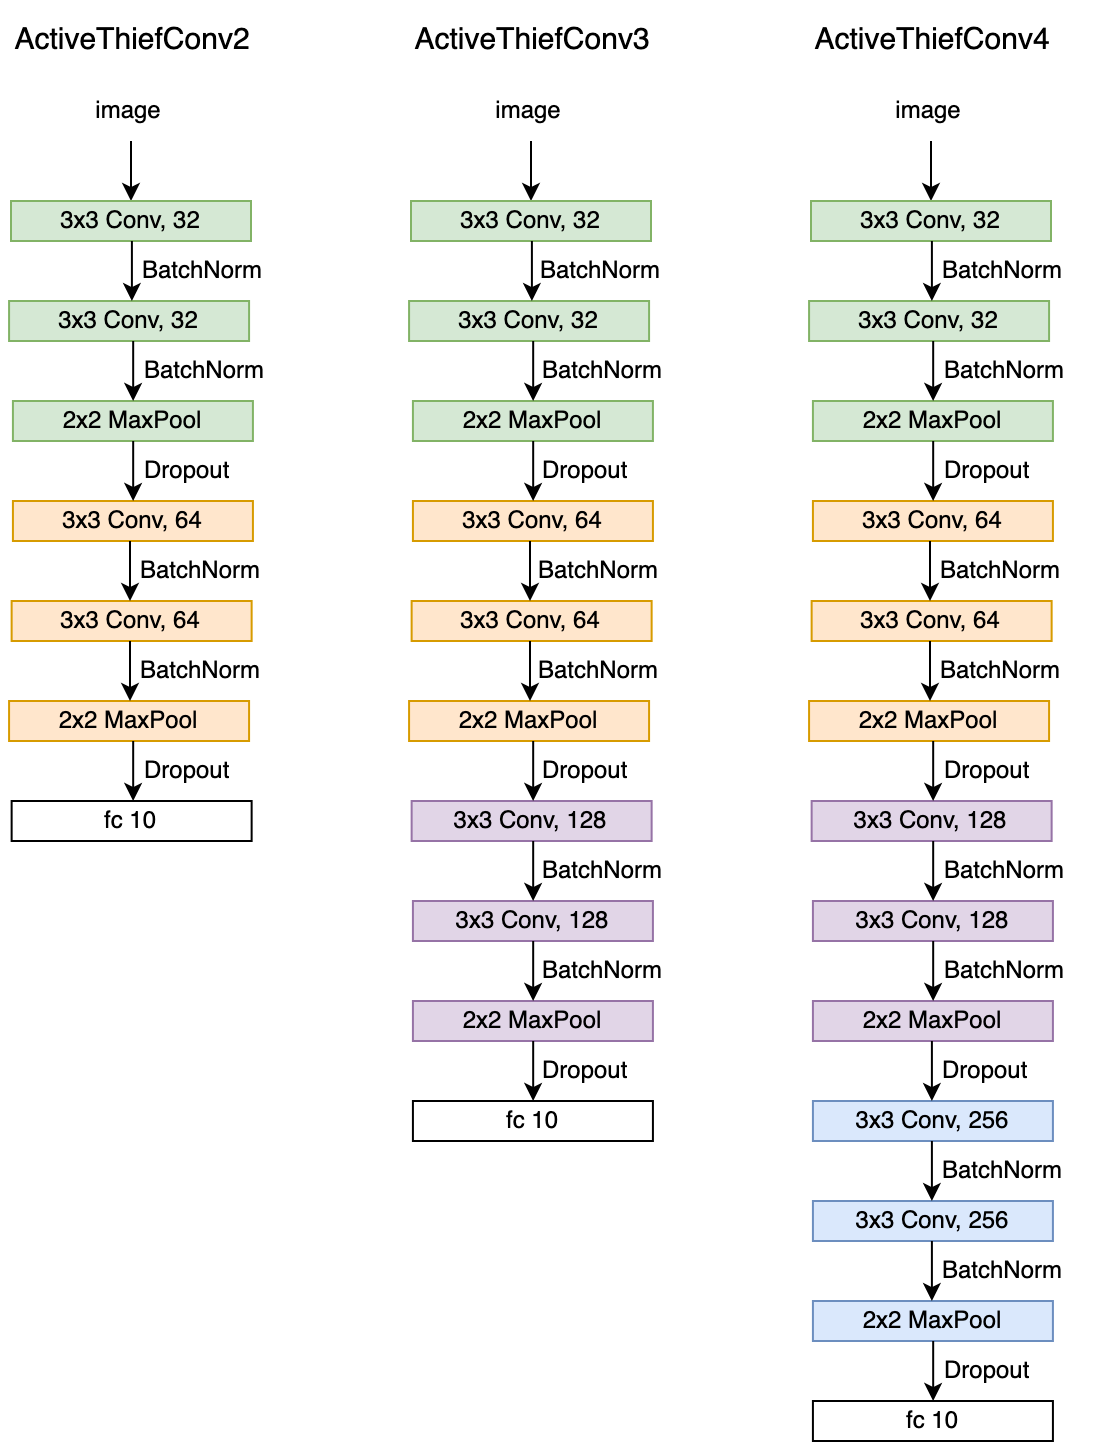
\includegraphics[width=\linewidth]{images/ActiveThiefConvs.png}
    \caption{Example network architectures for CIFAR-10.}
    \label{fig:ActiveThiefArchitectures}
\end{figure}

\clearpage

\section{Continual Active Learning}
\label{sec:Appendix:ContinualActiveLearning}
In section \ref{sec:Evaluation:CAL:ALRegCL}, we evaluate the performance of regularization-based continual learning strategies combined with the active learning
strategies Random, \gls{lc}, \gls{bald}, CoreSet and \gls{badge}. For space reasons, we omitted the results of our experiments for batch sizes 1,000 and 2,000 in 
the main paper. Therefore, we list the results for these batch sizes in the following. The results by validation accuracy are shown in figure
\ref{fig:Appendix:CAL:1000bAcc} and figure \ref{fig:Appendix:CAL:2000bAcc}, respectively. The execution time of these experiments is presented in table 
\ref{fig:Appendix:CAL:1000bTimeTable} and table \ref{fig:Appendix:CAL:2000bTimeTable}, respectively. \par
Overall, we observe similar patterns to the results presented in the main paper, regarding both the relative performance of the active learning strategies and
the continual learning strategies. However, the results for batch size 1,000 exhibit high variance, which is caused by overfitting on the small training set. 


\begin{figure}[h]
    \centering
    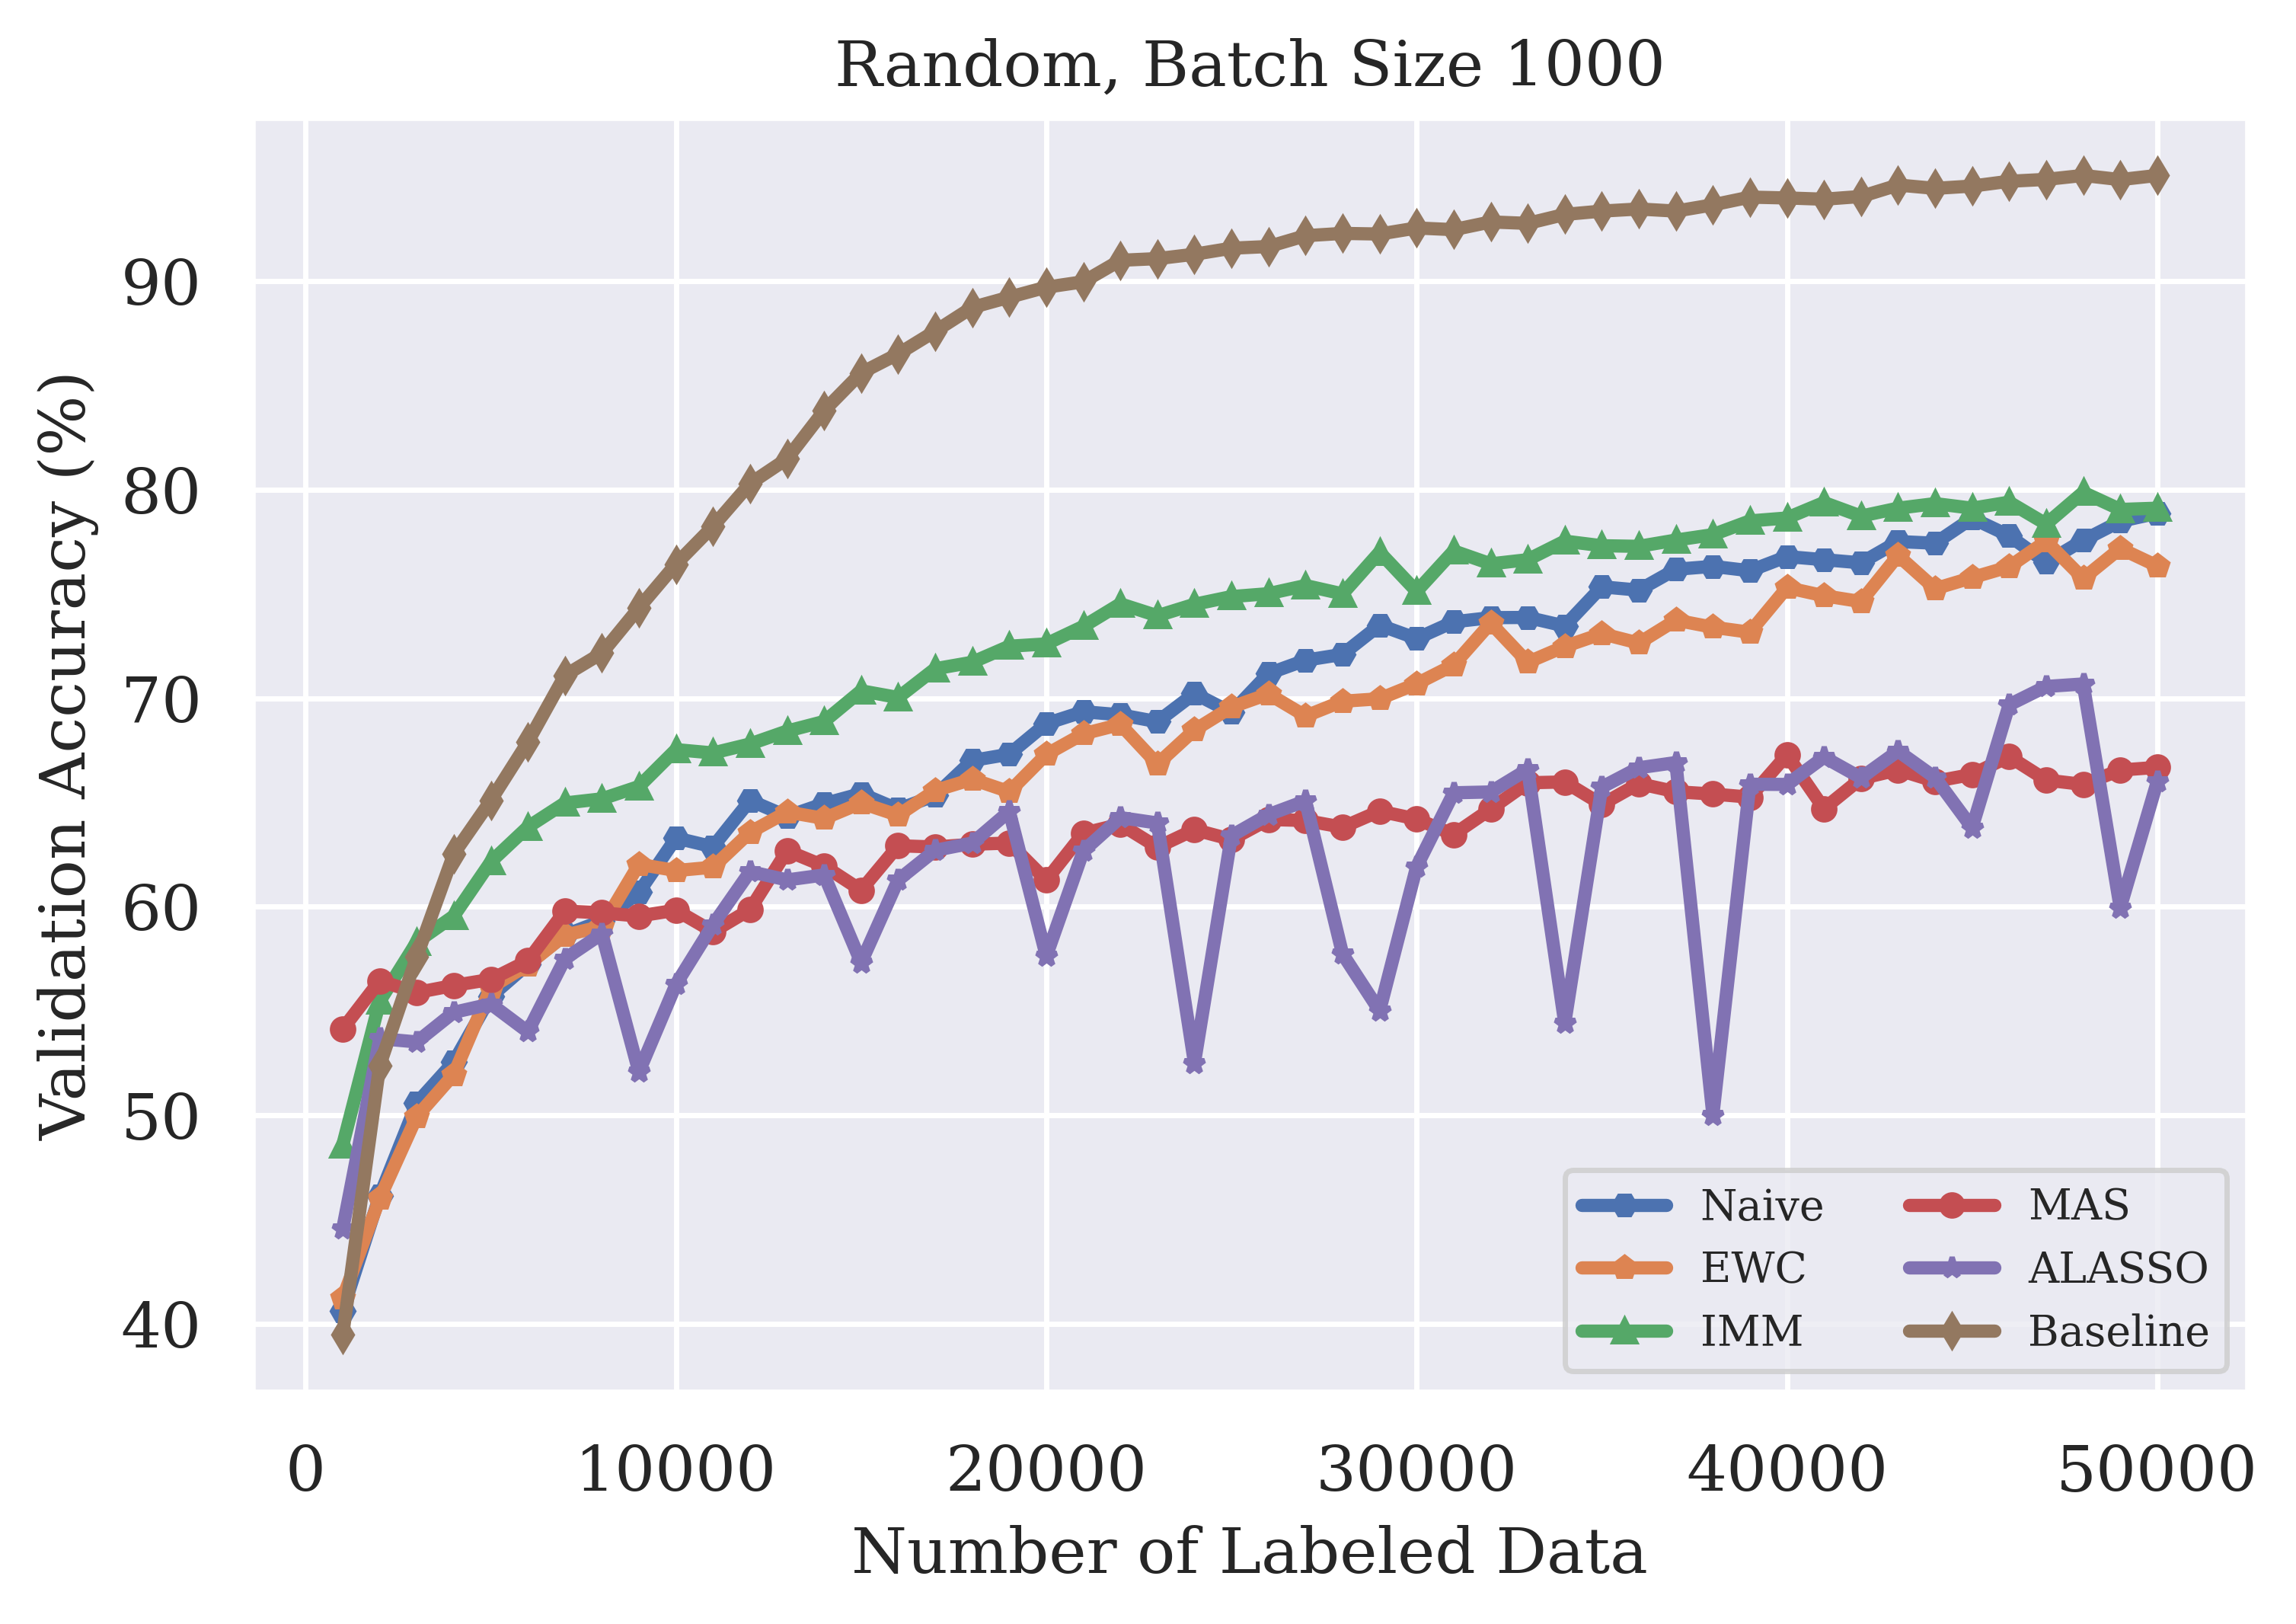
\includegraphics[width=0.32\linewidth]{images/results_CAL/random_1000b_acc.png} \hfill
    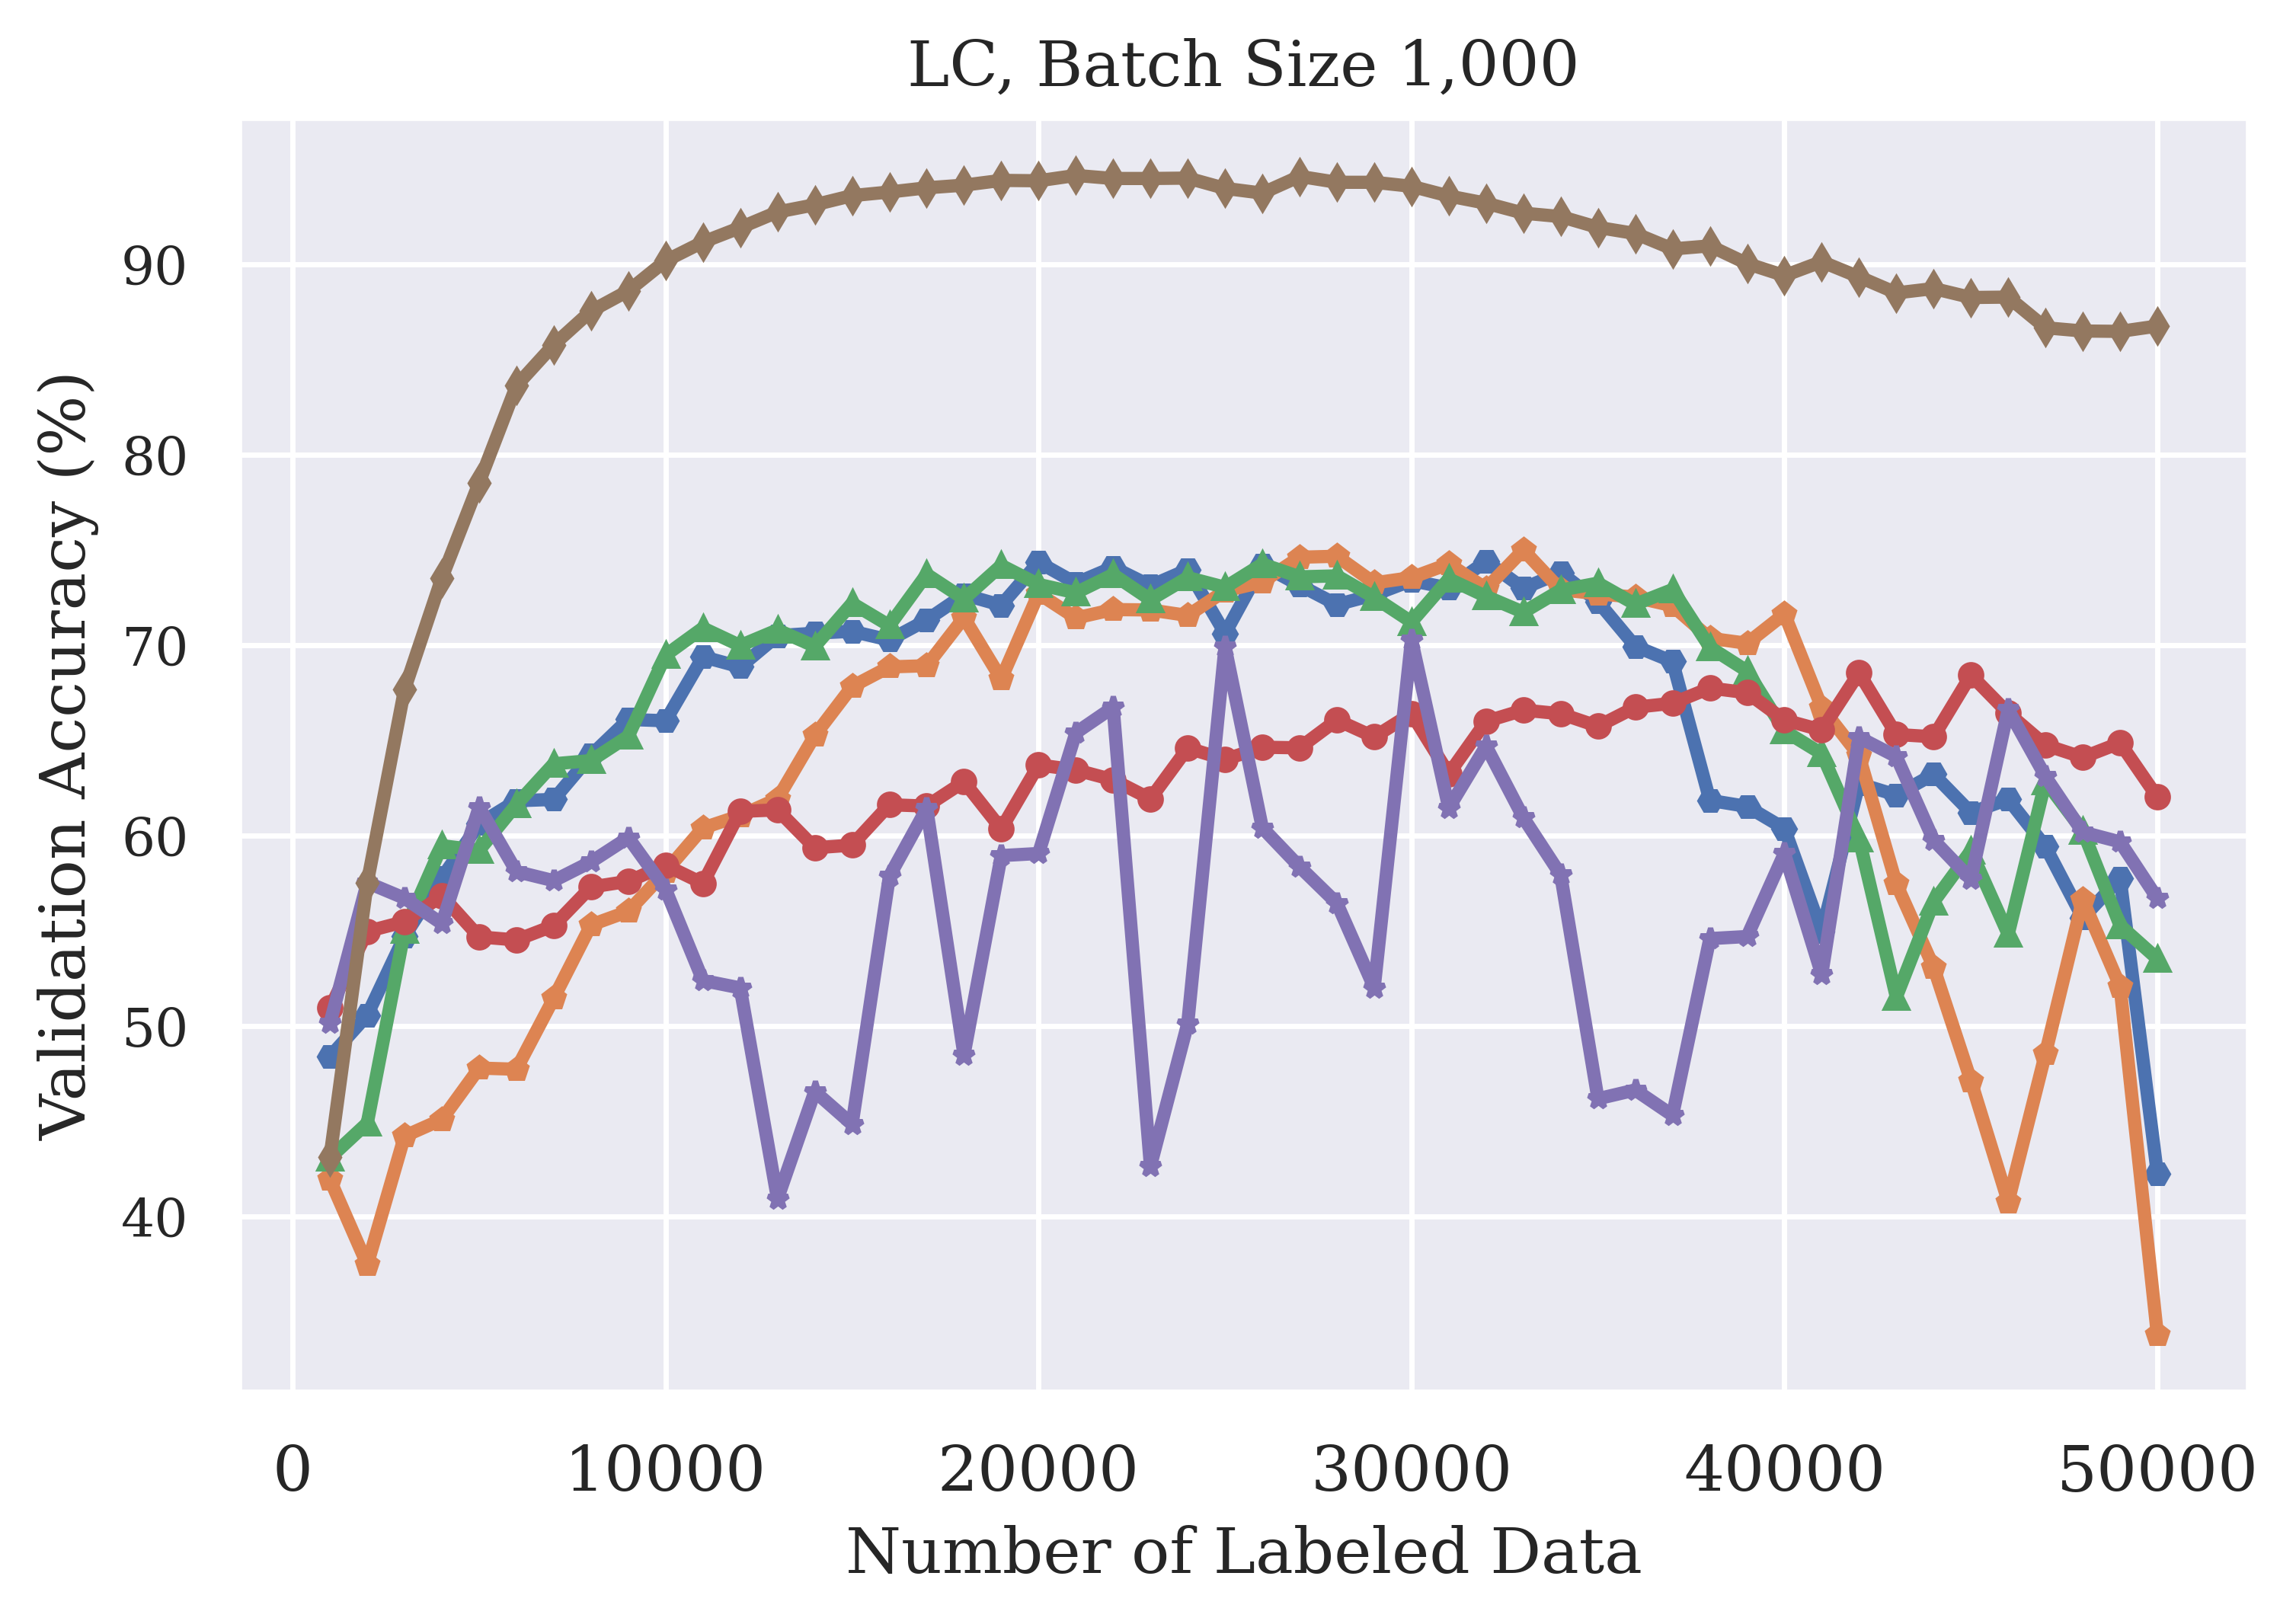
\includegraphics[width=0.32\linewidth]{images/results_CAL/lc_1000b_acc.png} \hfill
    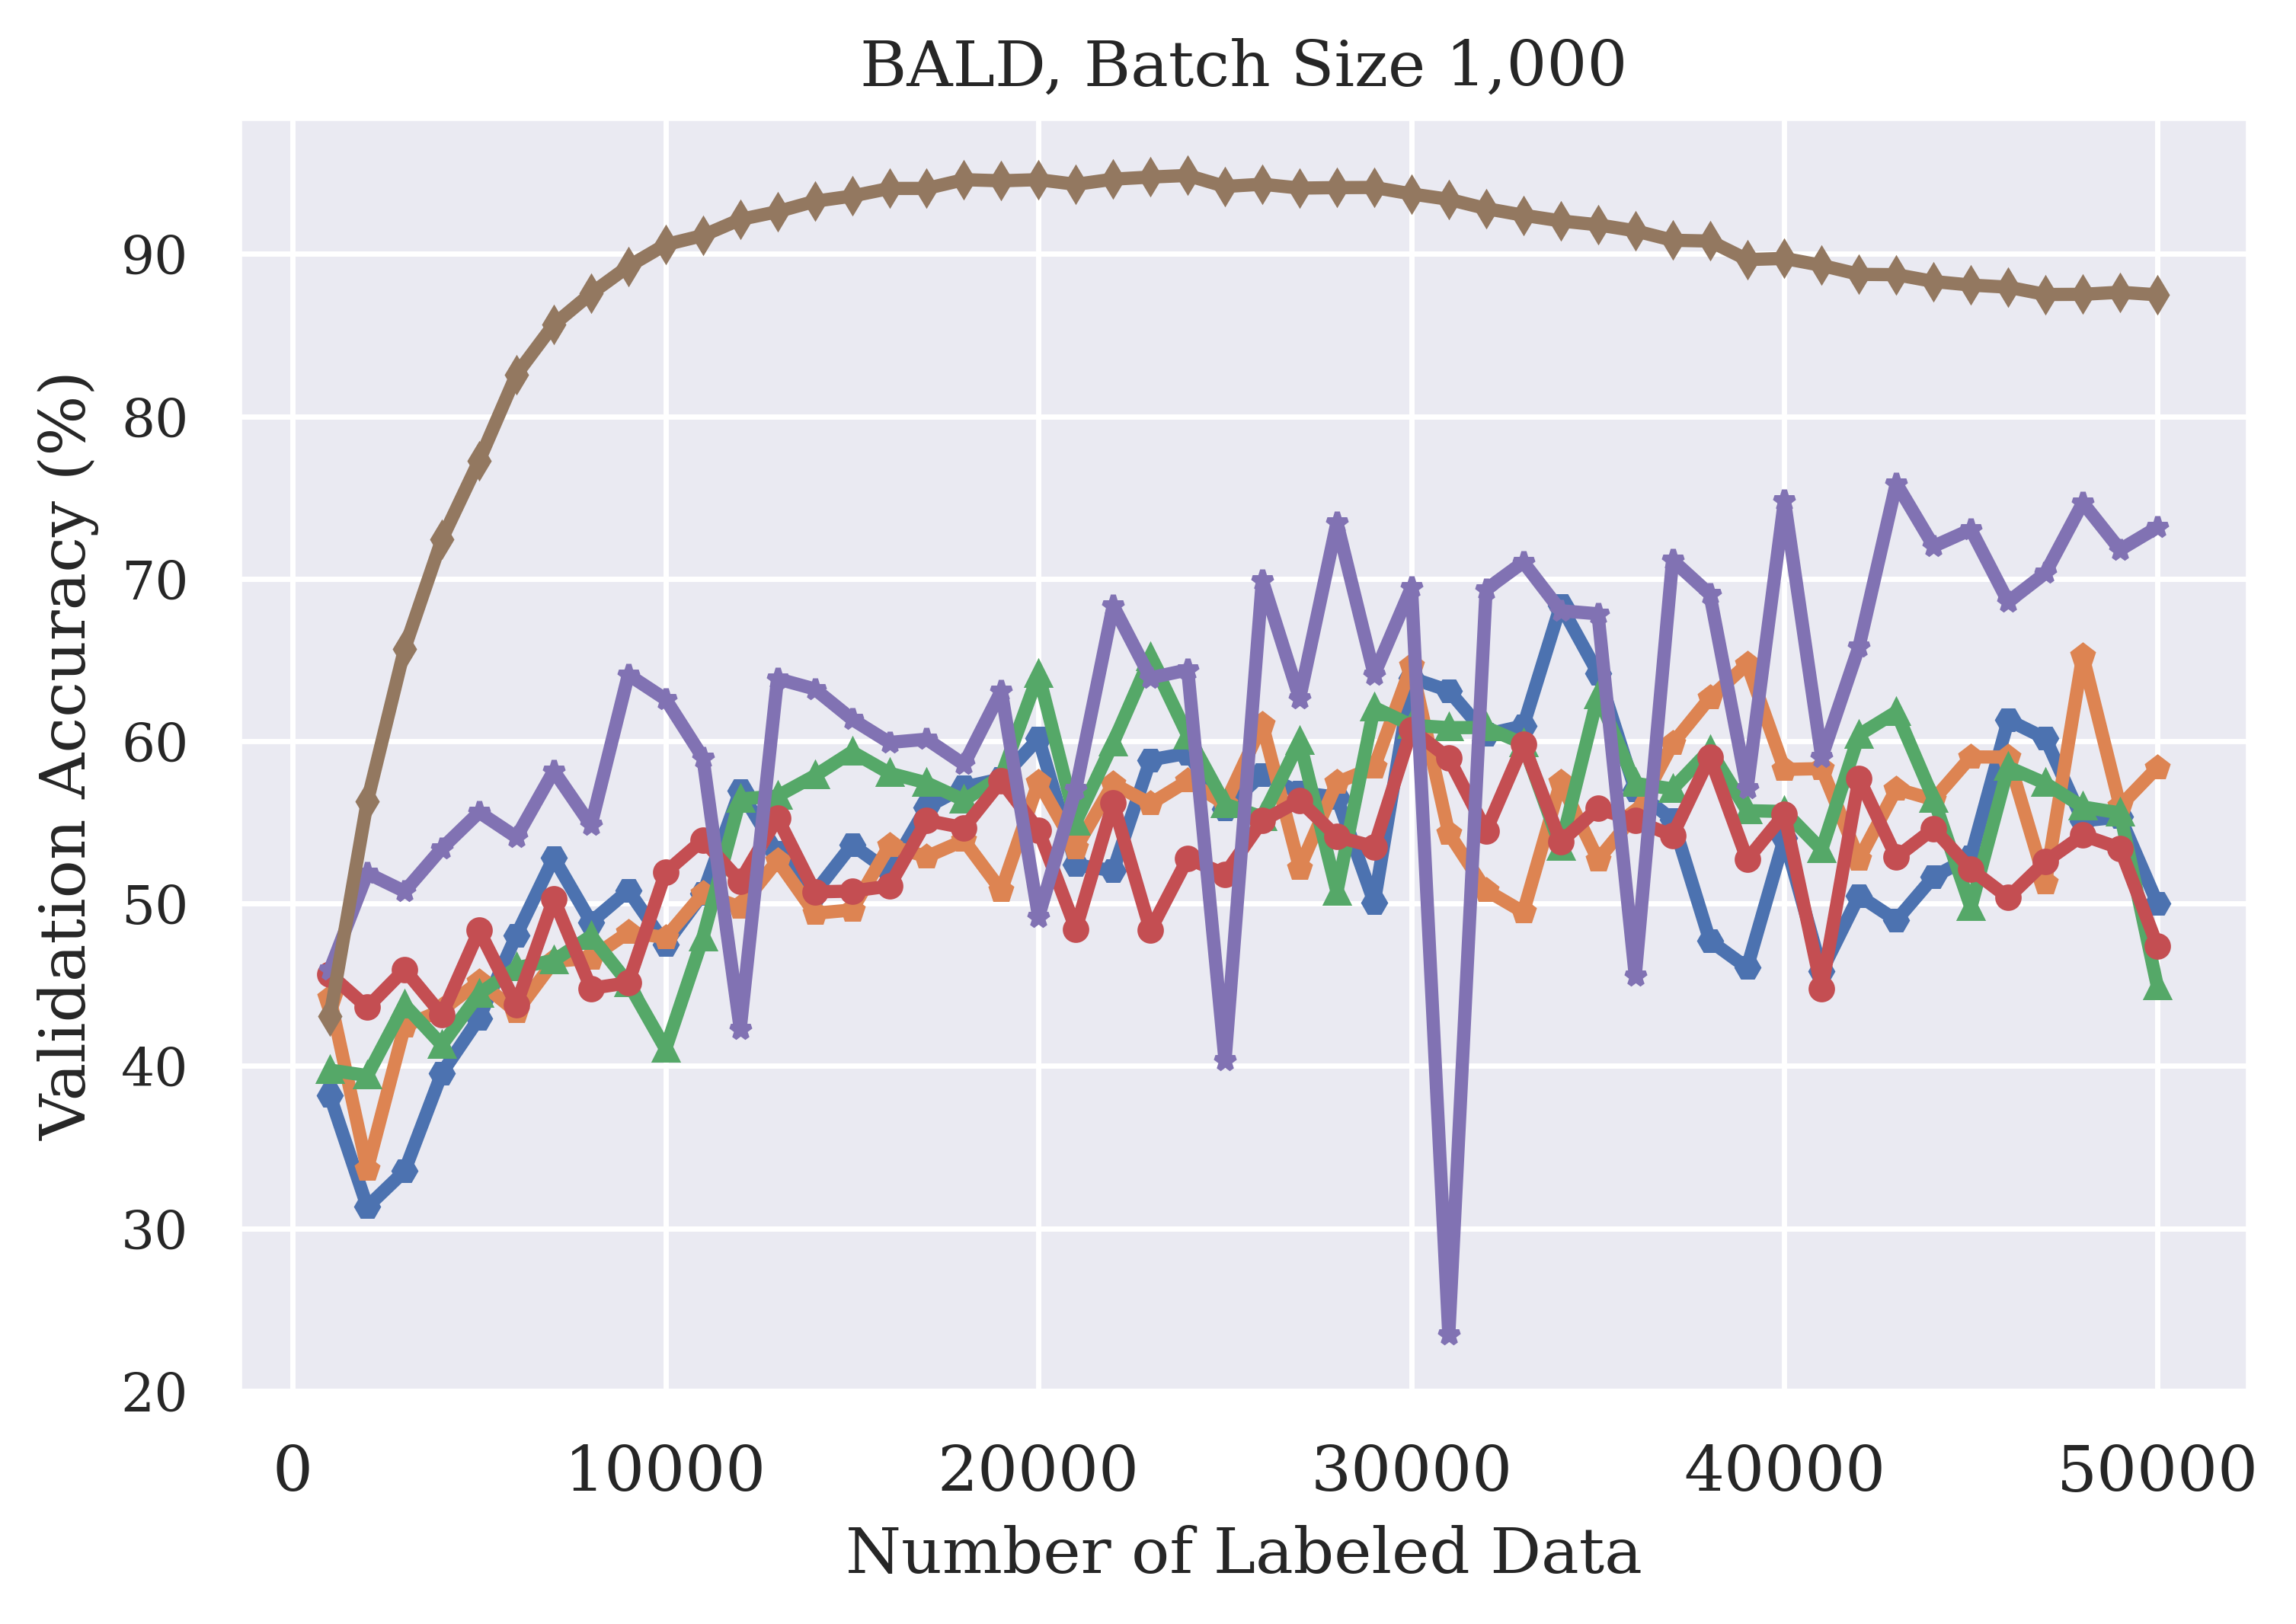
\includegraphics[width=0.32\linewidth]{images/results_CAL/bald_1000b_acc.png}
    \\[\smallskipamount]
    \hfill 
    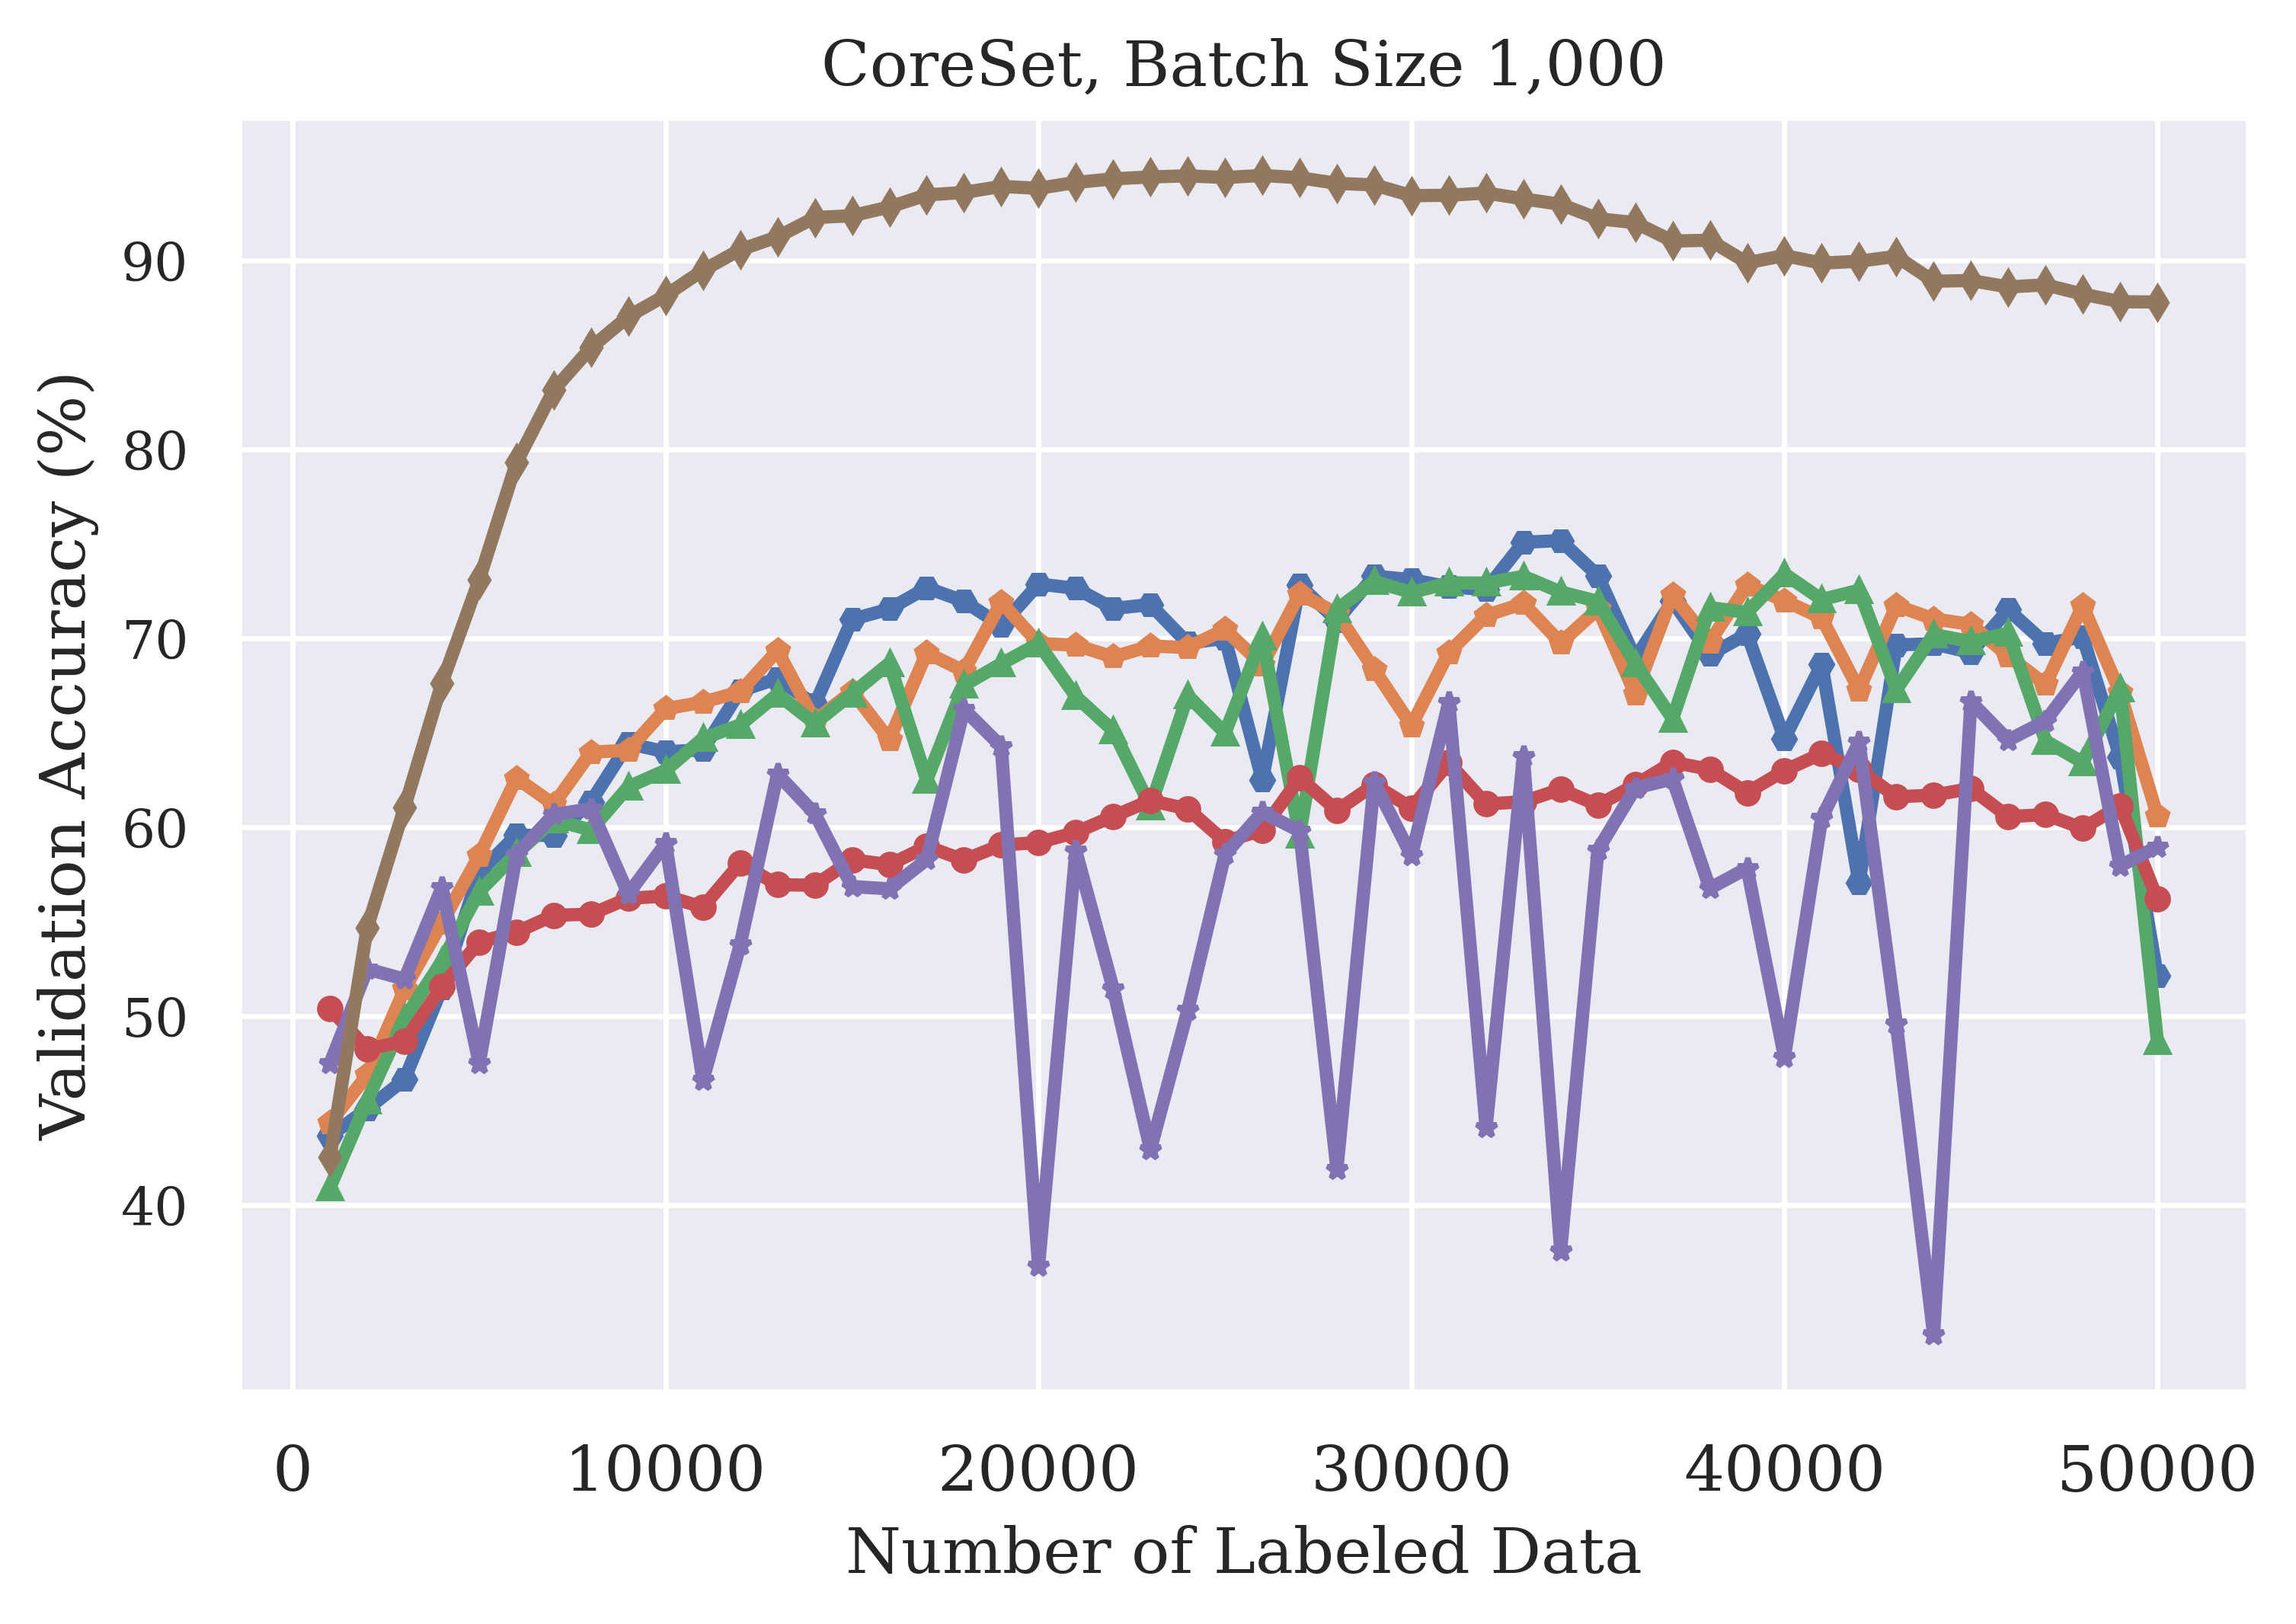
\includegraphics[width=0.32\linewidth]{images/results_CAL/coreset_1000b_acc.png} \hfill
    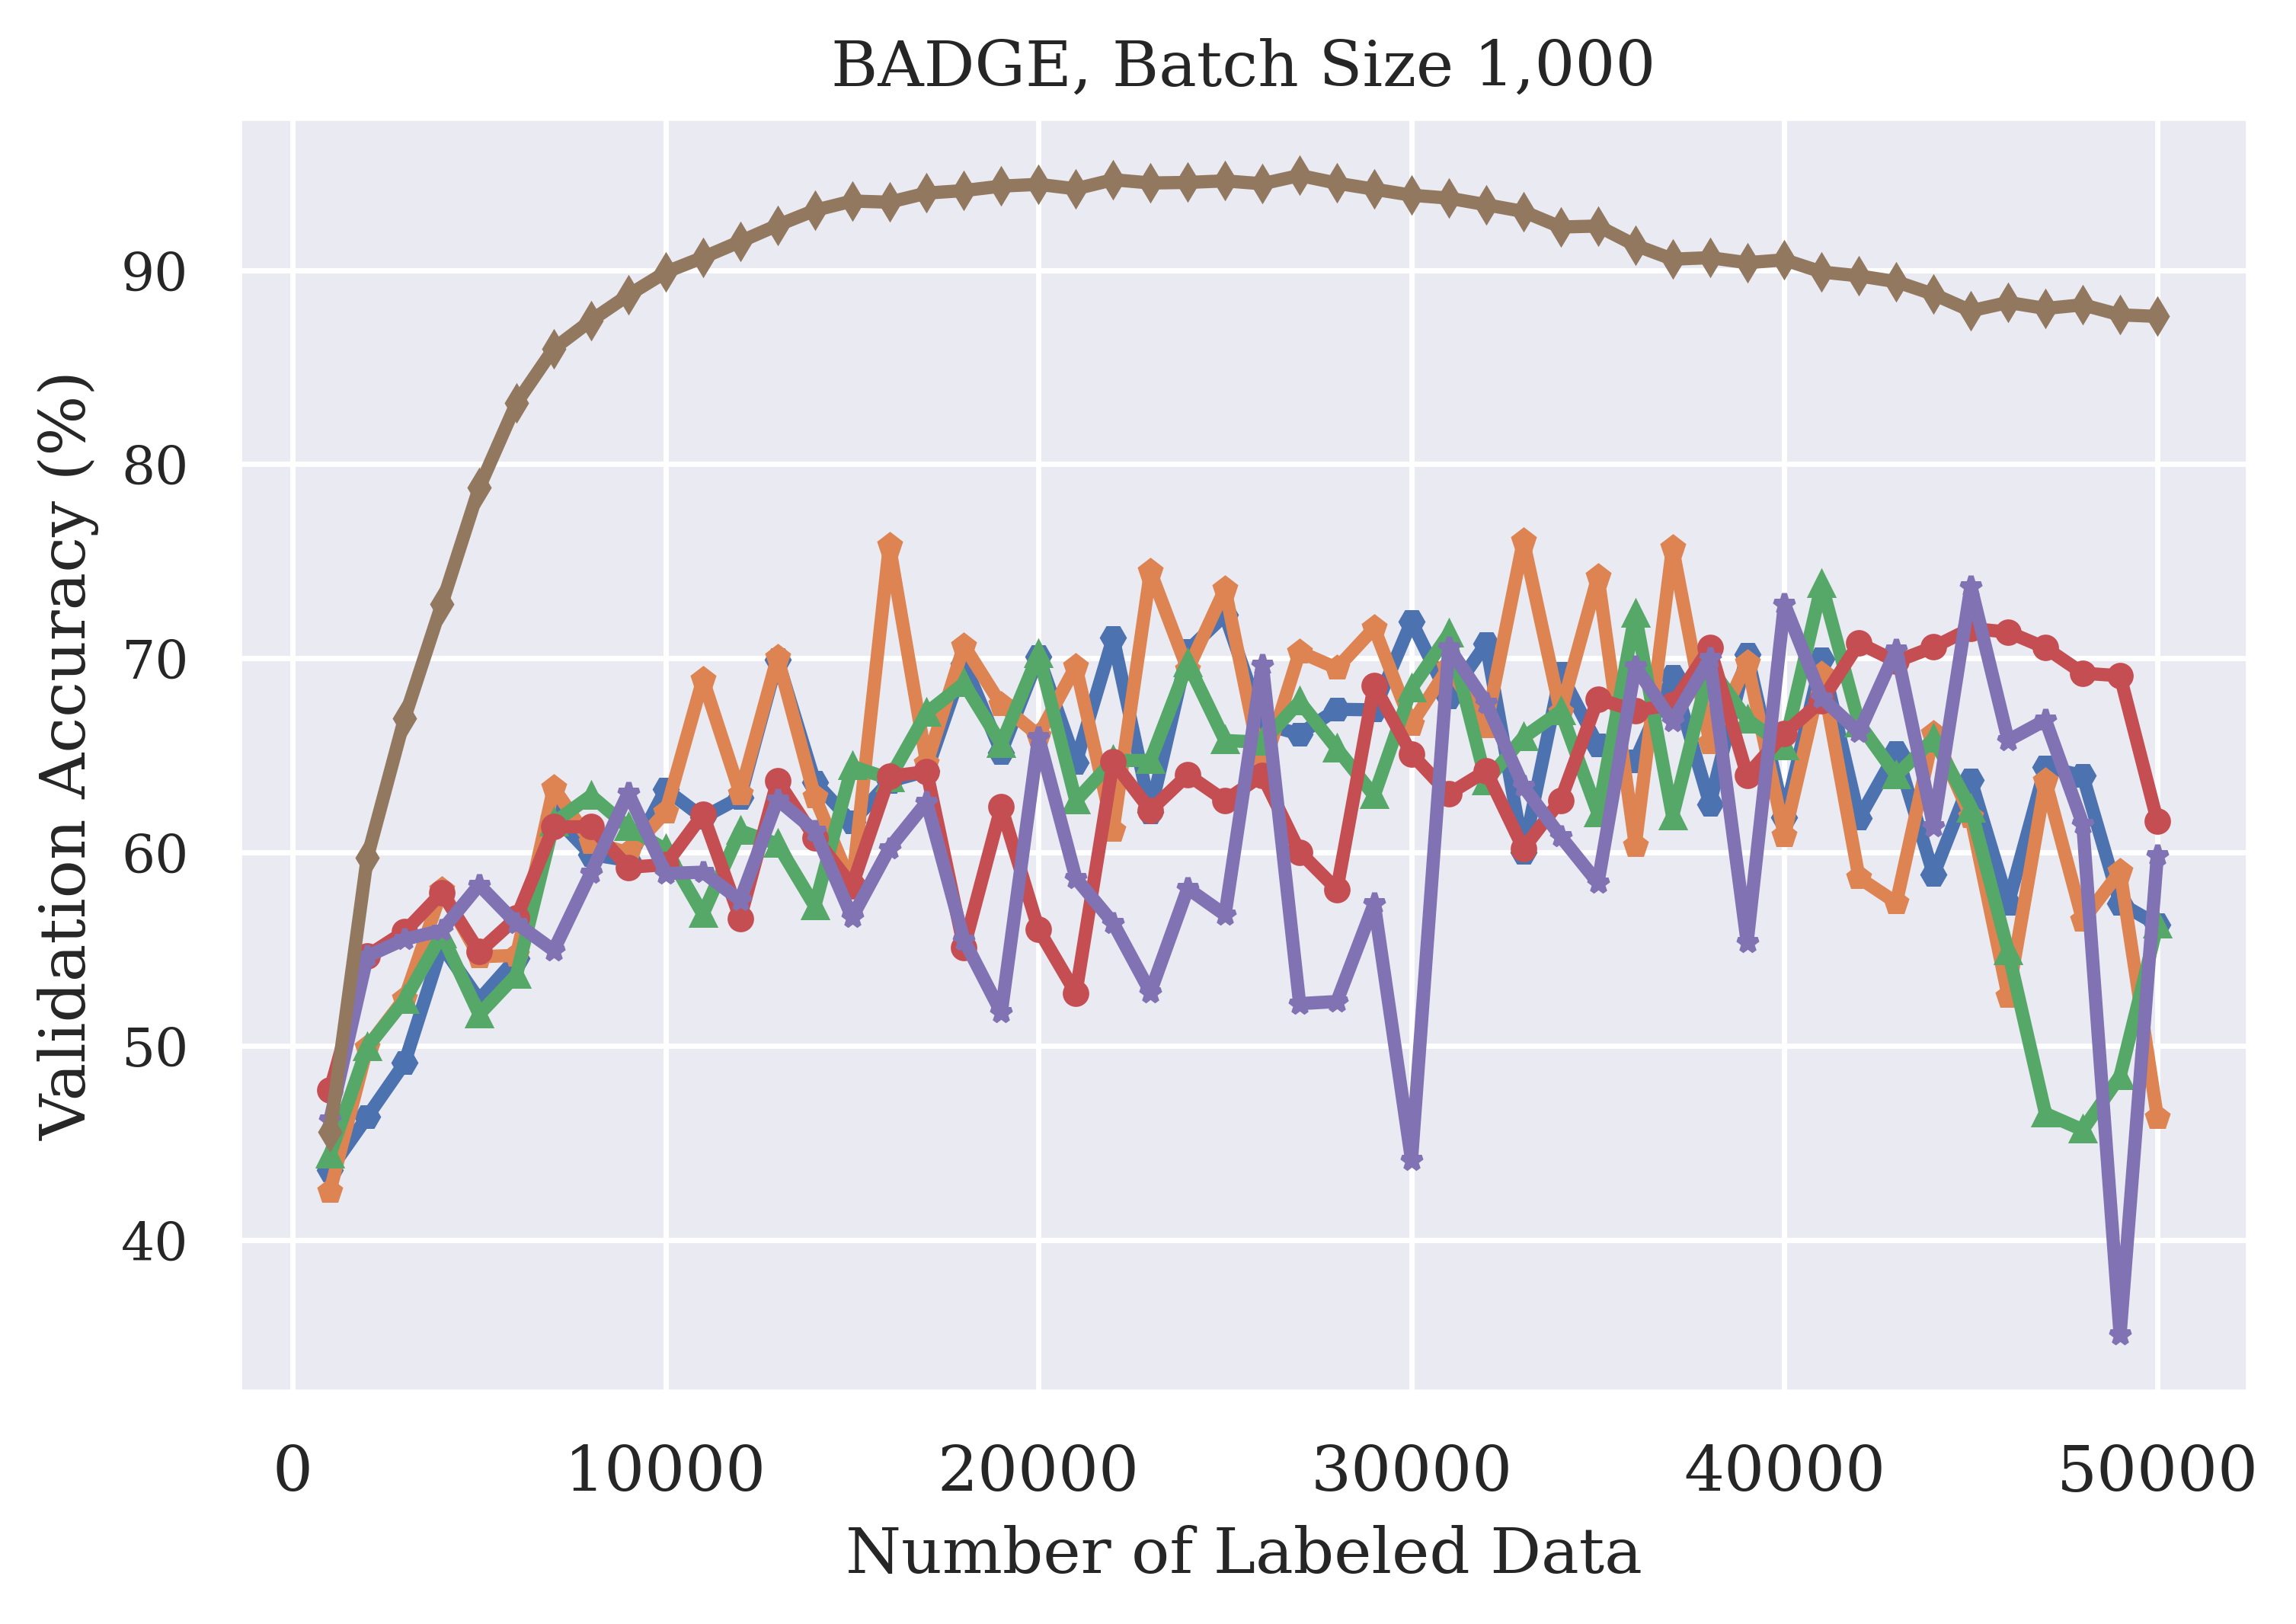
\includegraphics[width=0.32\linewidth]{images/results_CAL/badge_1000b_acc.png} \hfill
    \caption[Continual active learning with \gls{badge} with batch size 1,000]{Comparison of validation accuracy of continual active earning strategies
    with batch size 1,000.}
    \label{fig:Appendix:CAL:1000bAcc}
\end{figure}

\begin{table}[h]
    \centering
    \begin{tabular}{c | c c c c c } 
         & Random & \gls{lc} & \gls{bald} & CoreSet & \gls{badge}\\ 
        \hline 
        Baseline & 2,522 & 2,536 & 2,549 & 2,650 & 3,171 \\
        \hline
        Naive & 44 & 50 & 50 & 144 & 493 \\
        \gls{ewc} & 44 & 53 & 51 & 140 & 486\\
        \gls{imm} & 42 & 49 & 48 & 137 & 501\\
        \gls{mas} & 48 & 55 & 53 & 147 & 505\\
        \gls{alasso} & 68 & 75 & 75 & 168 & 509\\
    \end{tabular}
    \caption{Comparison of execution time of regularization-based continual learning strategies
    with batch size 1,000.}
    \label{fig:Appendix:CAL:1000bTimeTable}
\end{table}


\begin{figure}[h]
    \centering
    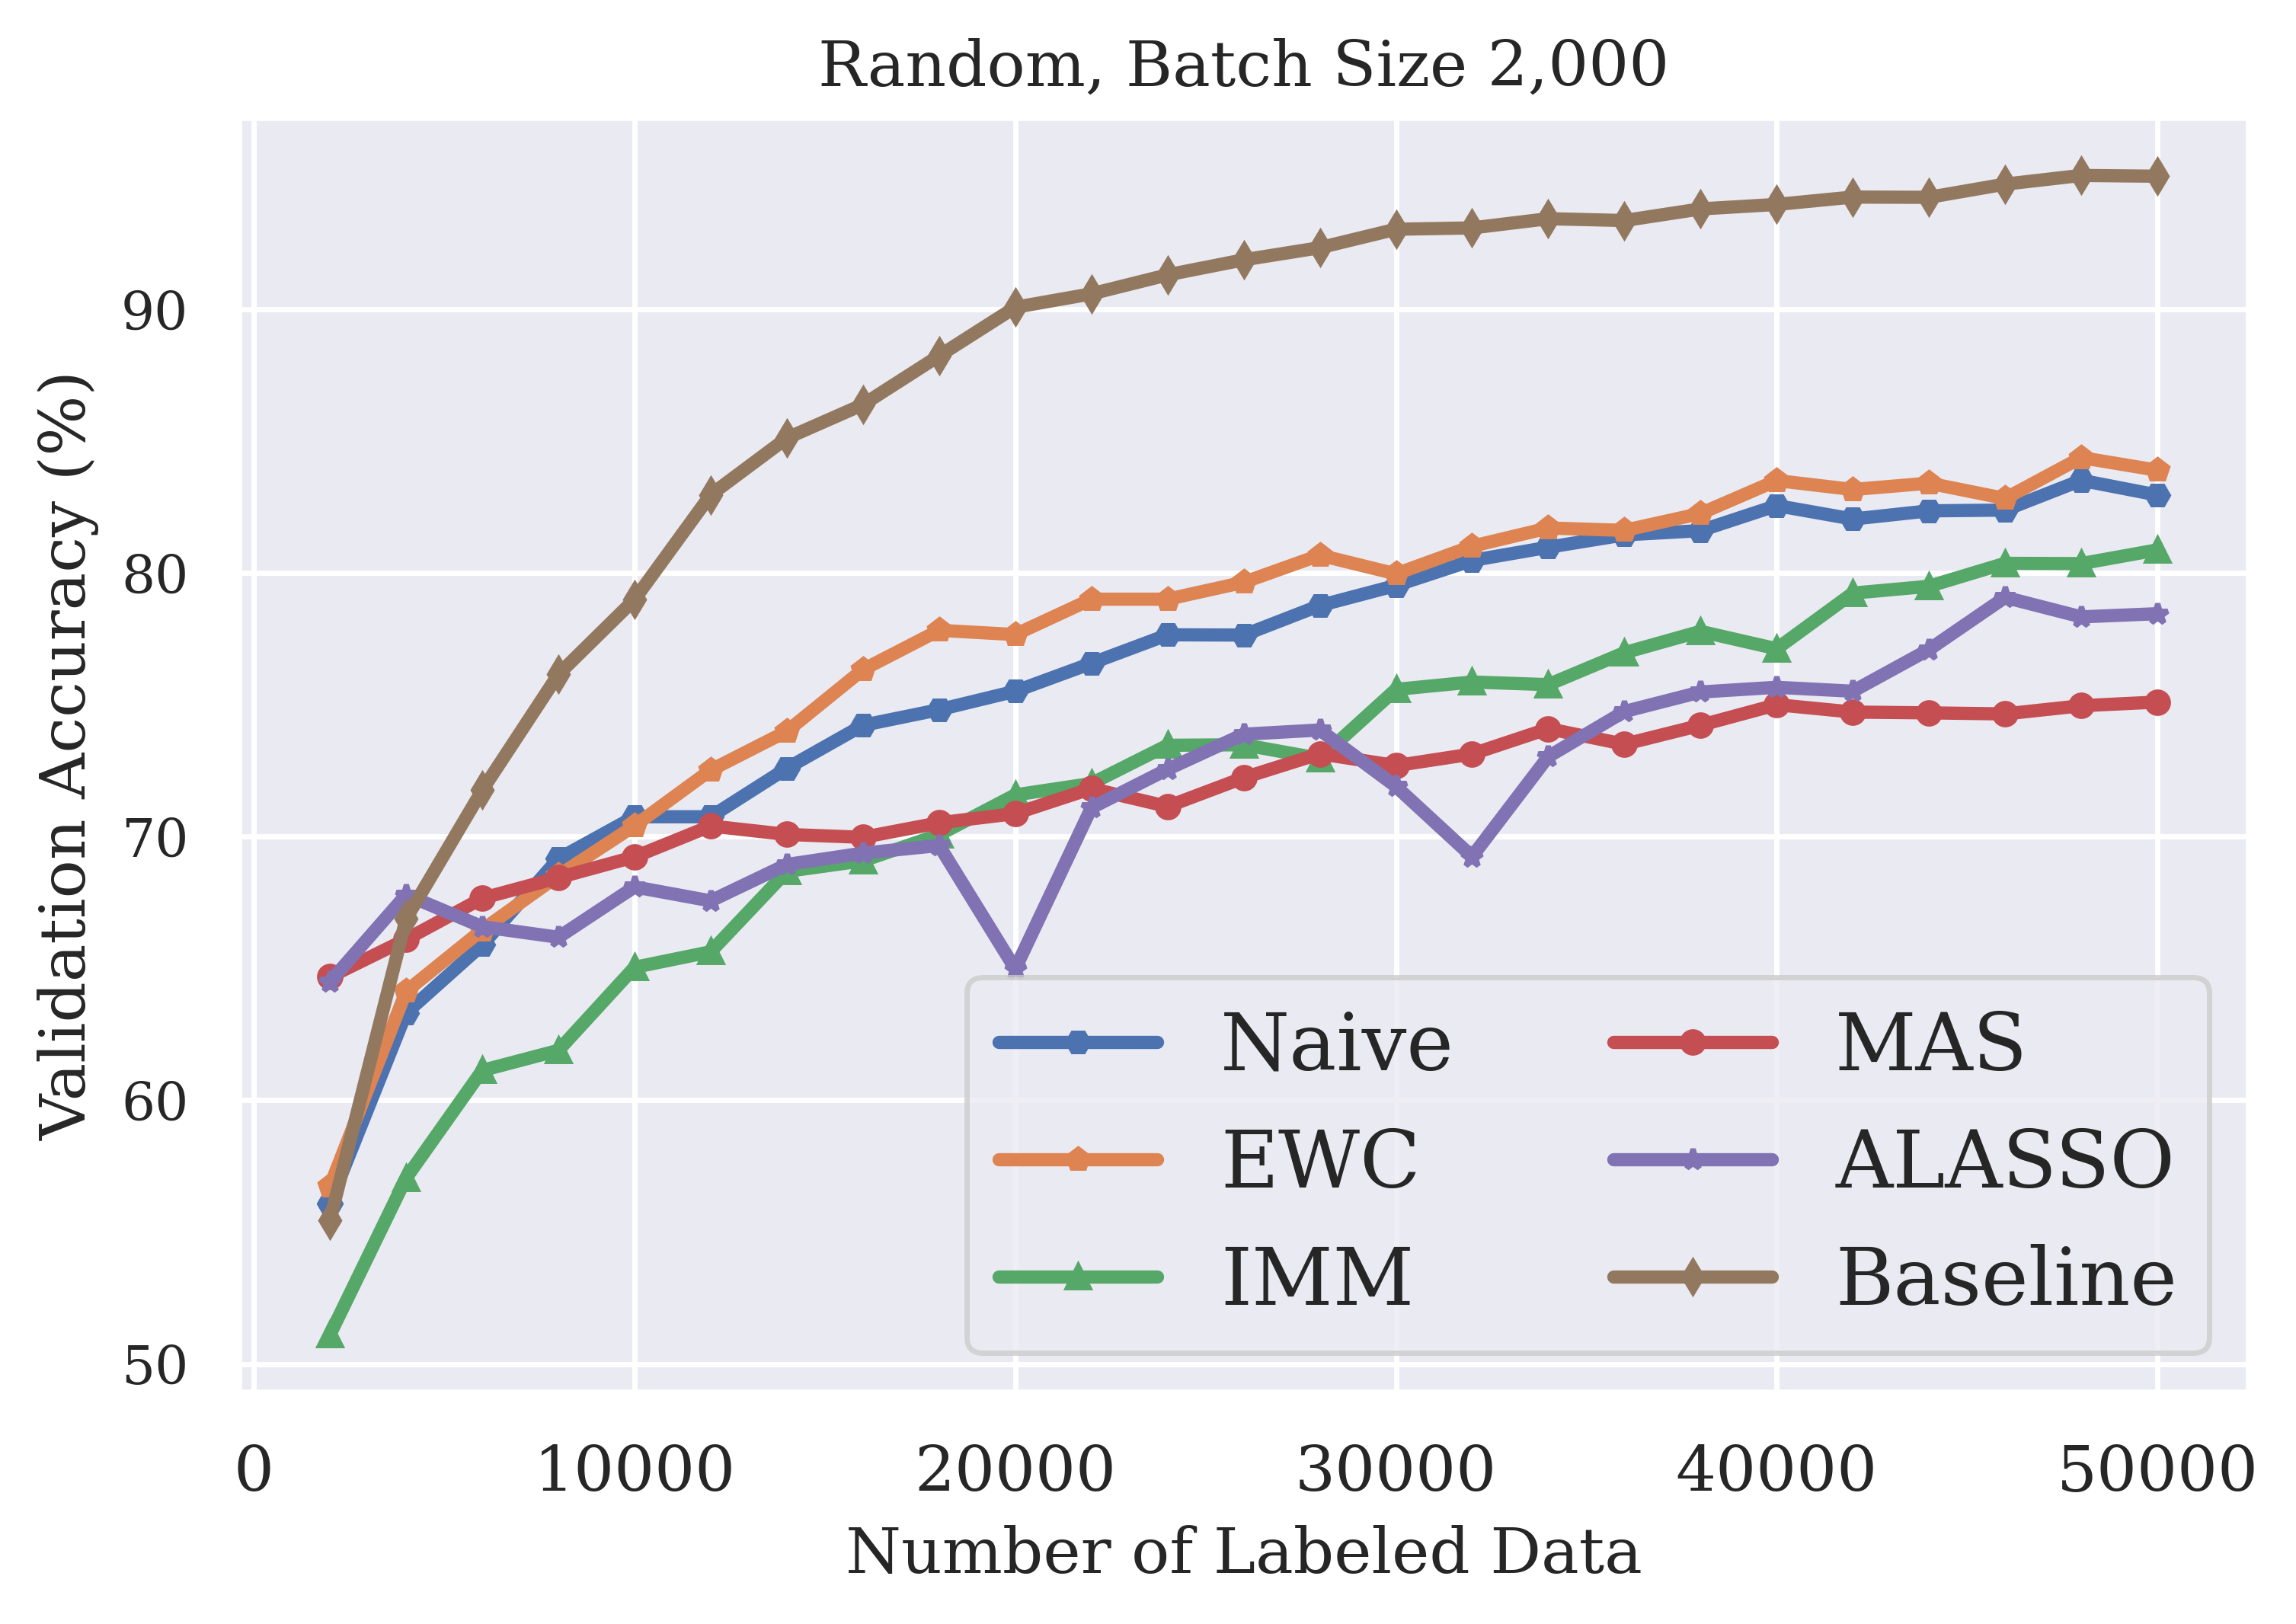
\includegraphics[width=0.32\linewidth]{images/results_CAL/random_2000b_acc.png} \hfill
    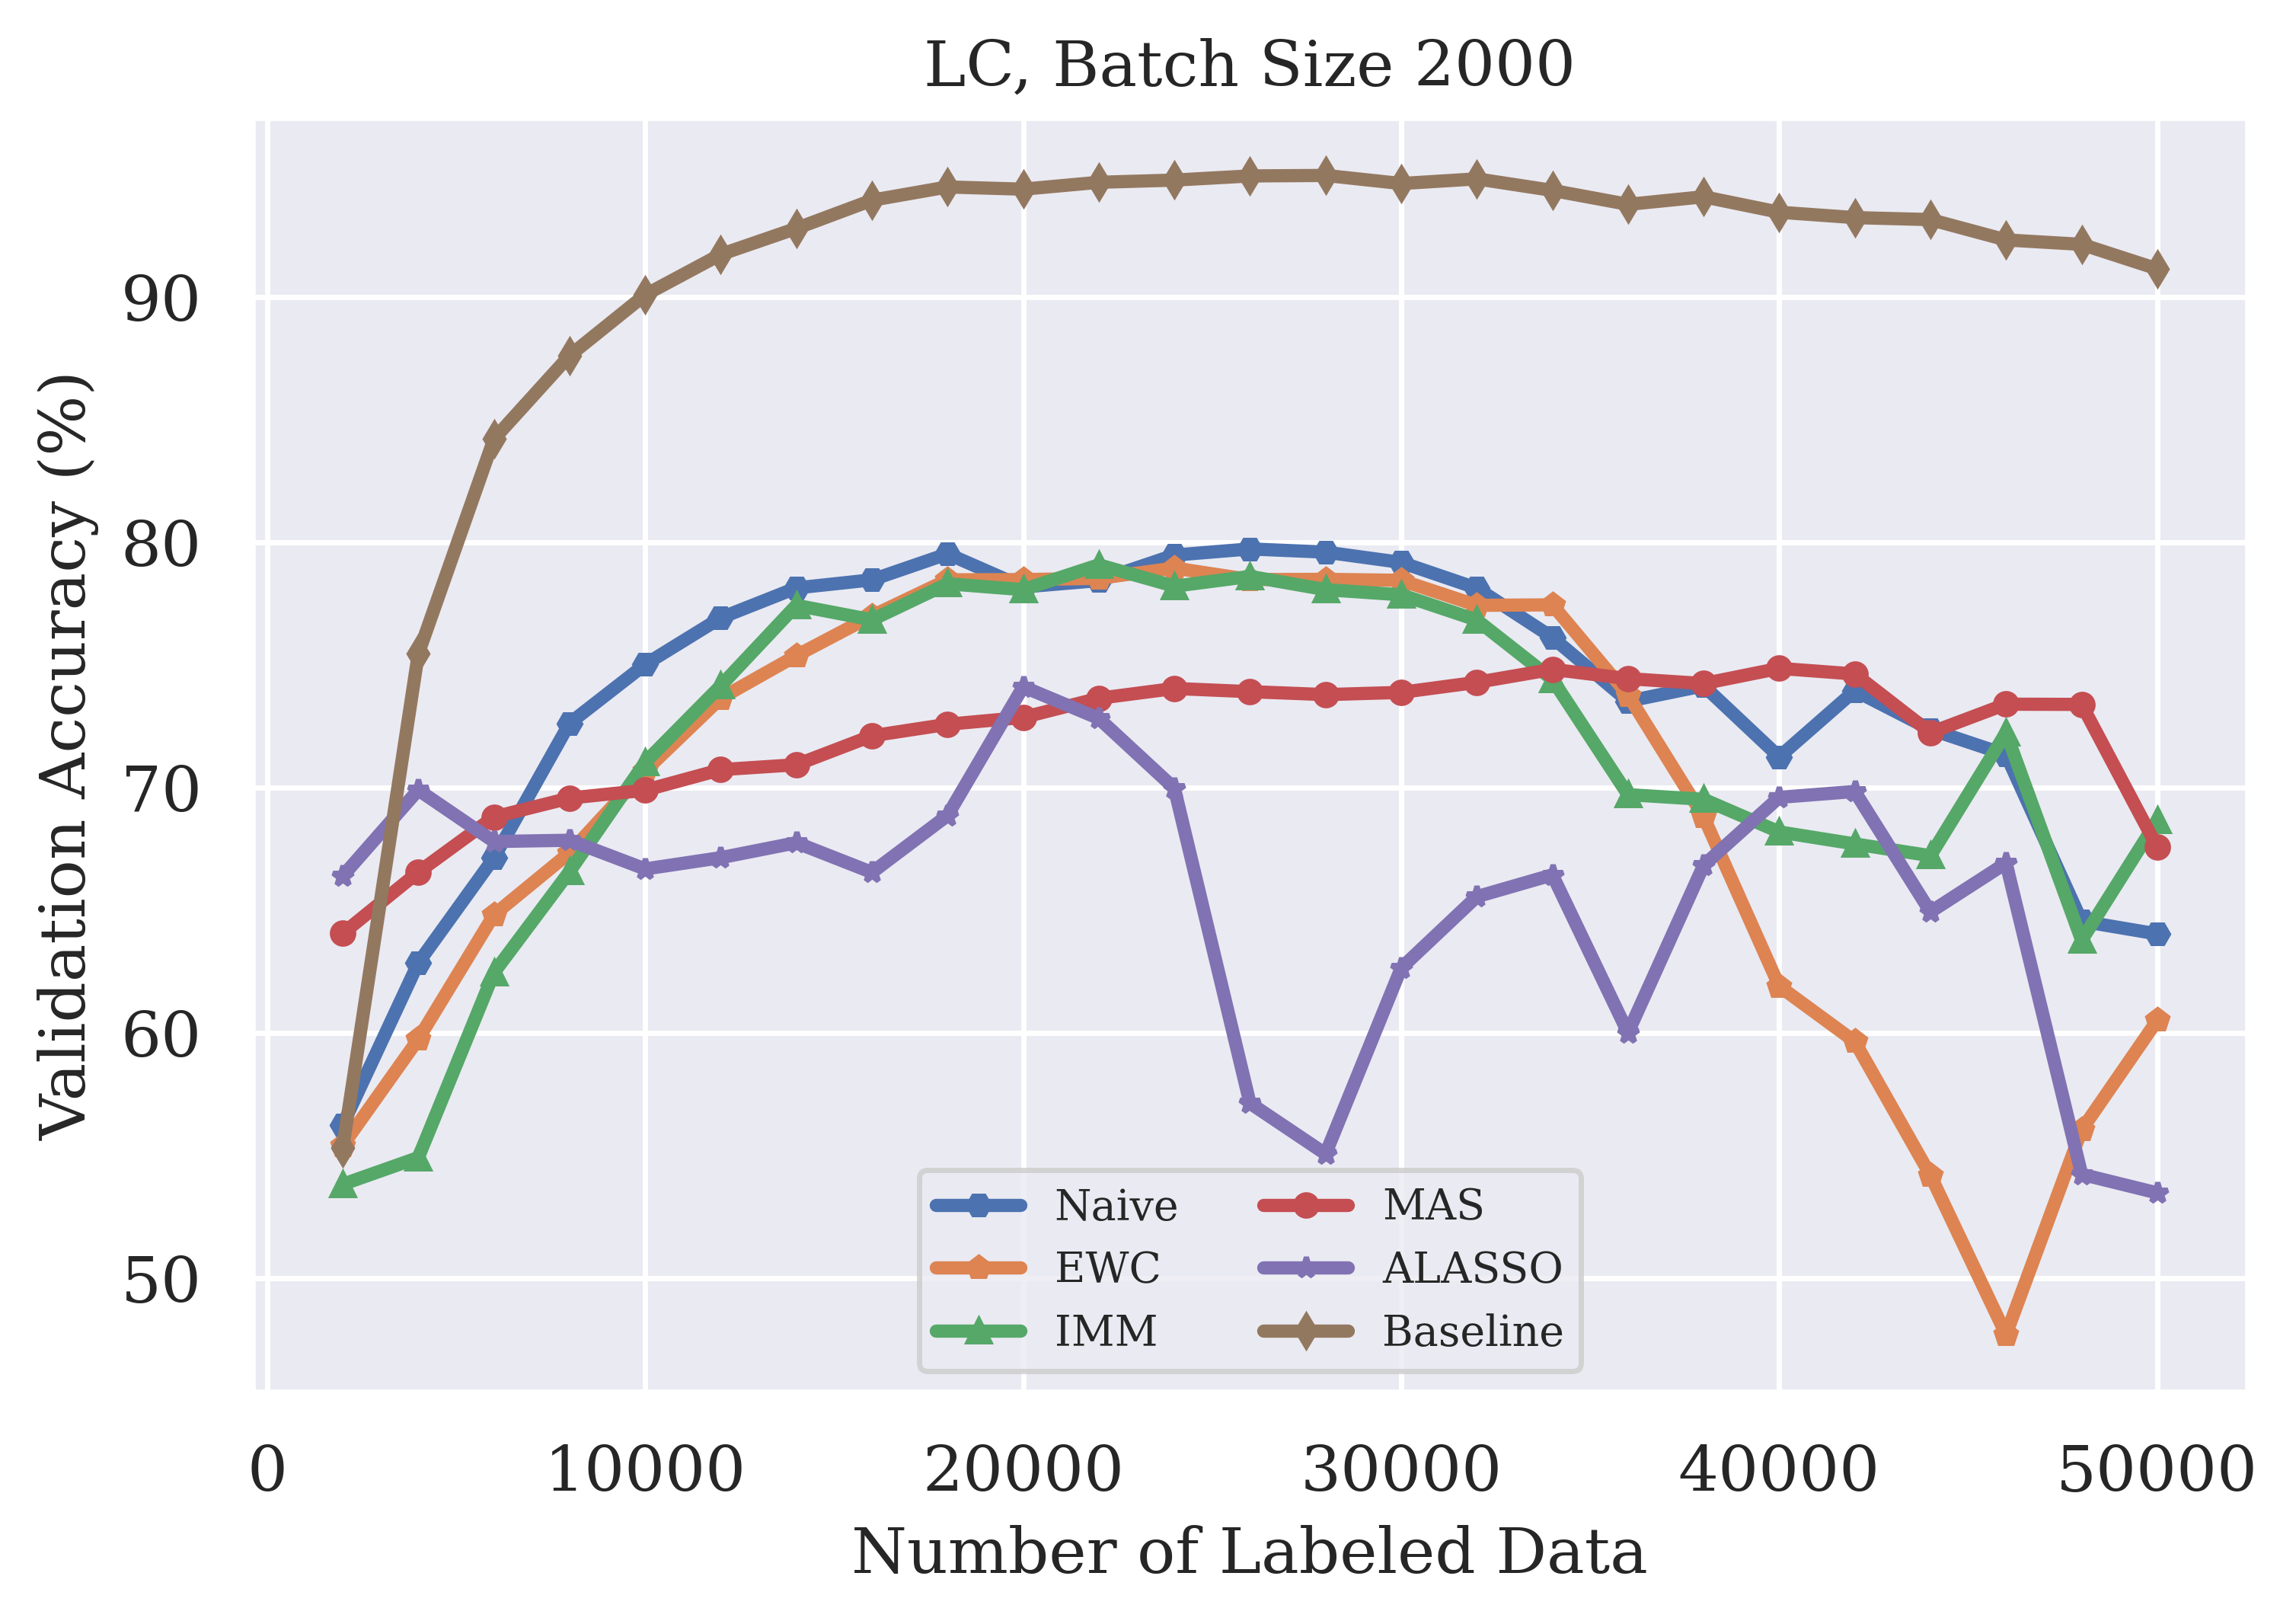
\includegraphics[width=0.32\linewidth]{images/results_CAL/lc_2000b_acc.png} \hfill
    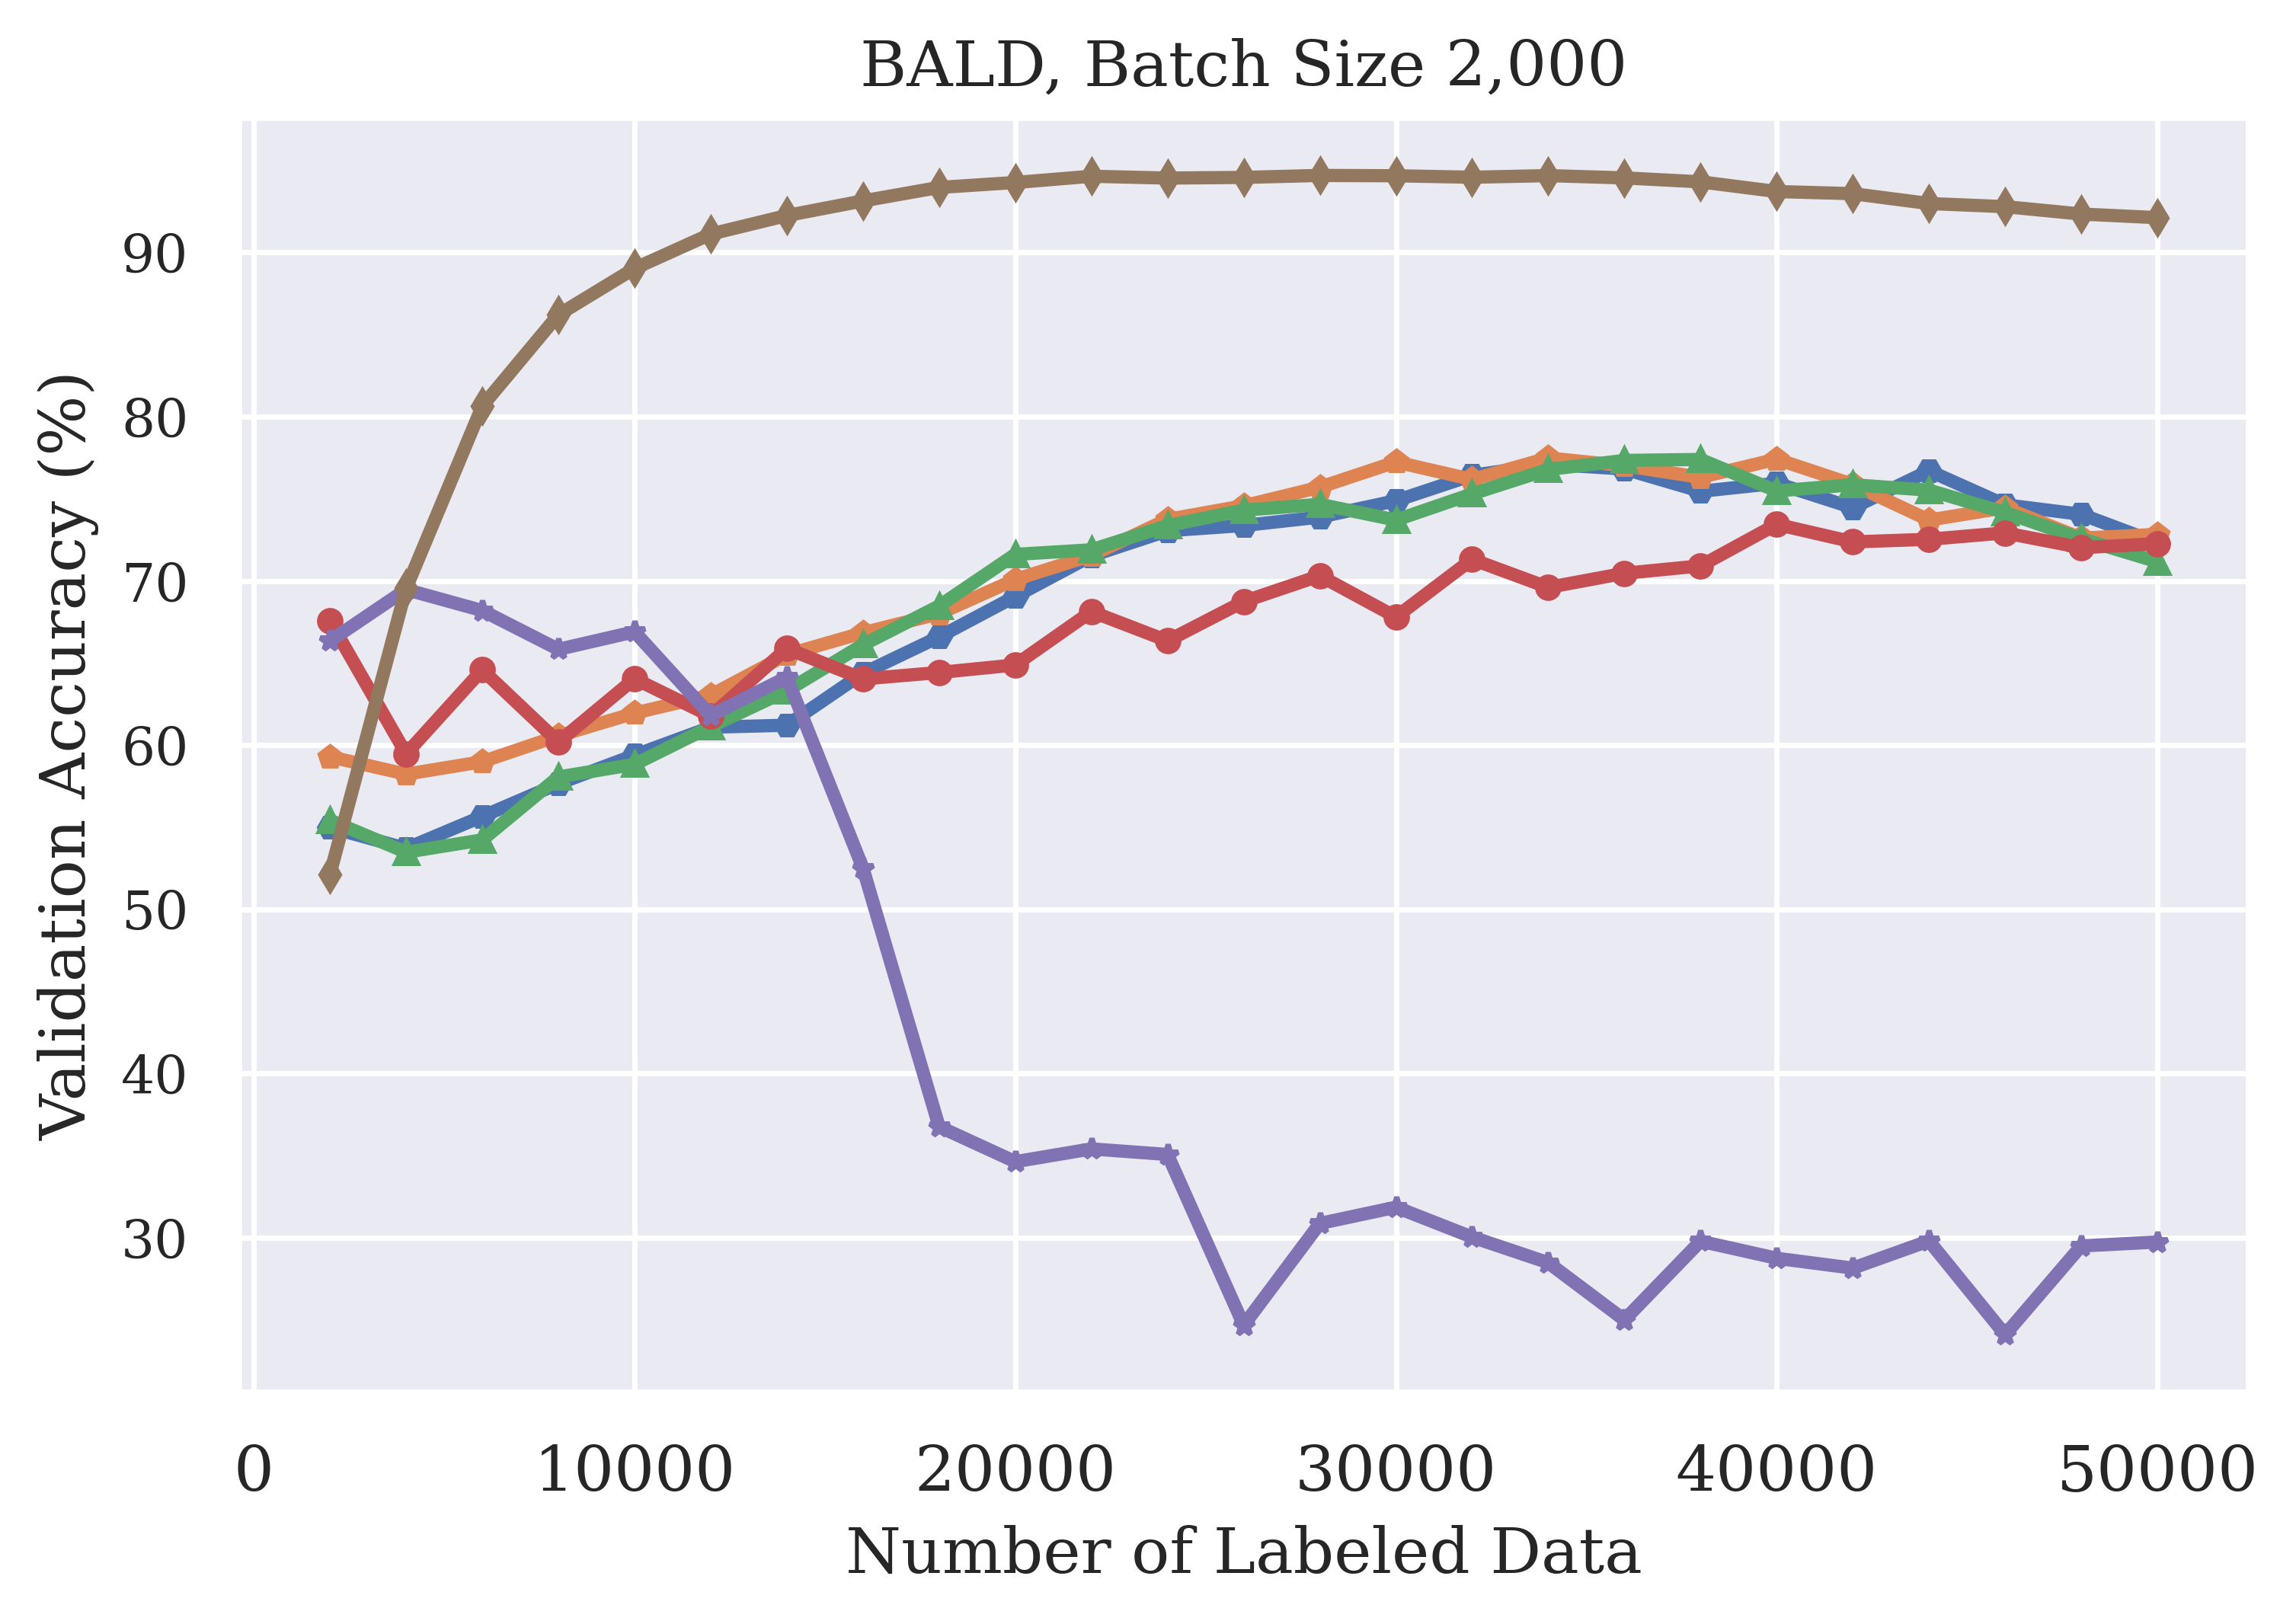
\includegraphics[width=0.32\linewidth]{images/results_CAL/bald_2000b_acc.png}
    \\[\smallskipamount]
    \hfill 
    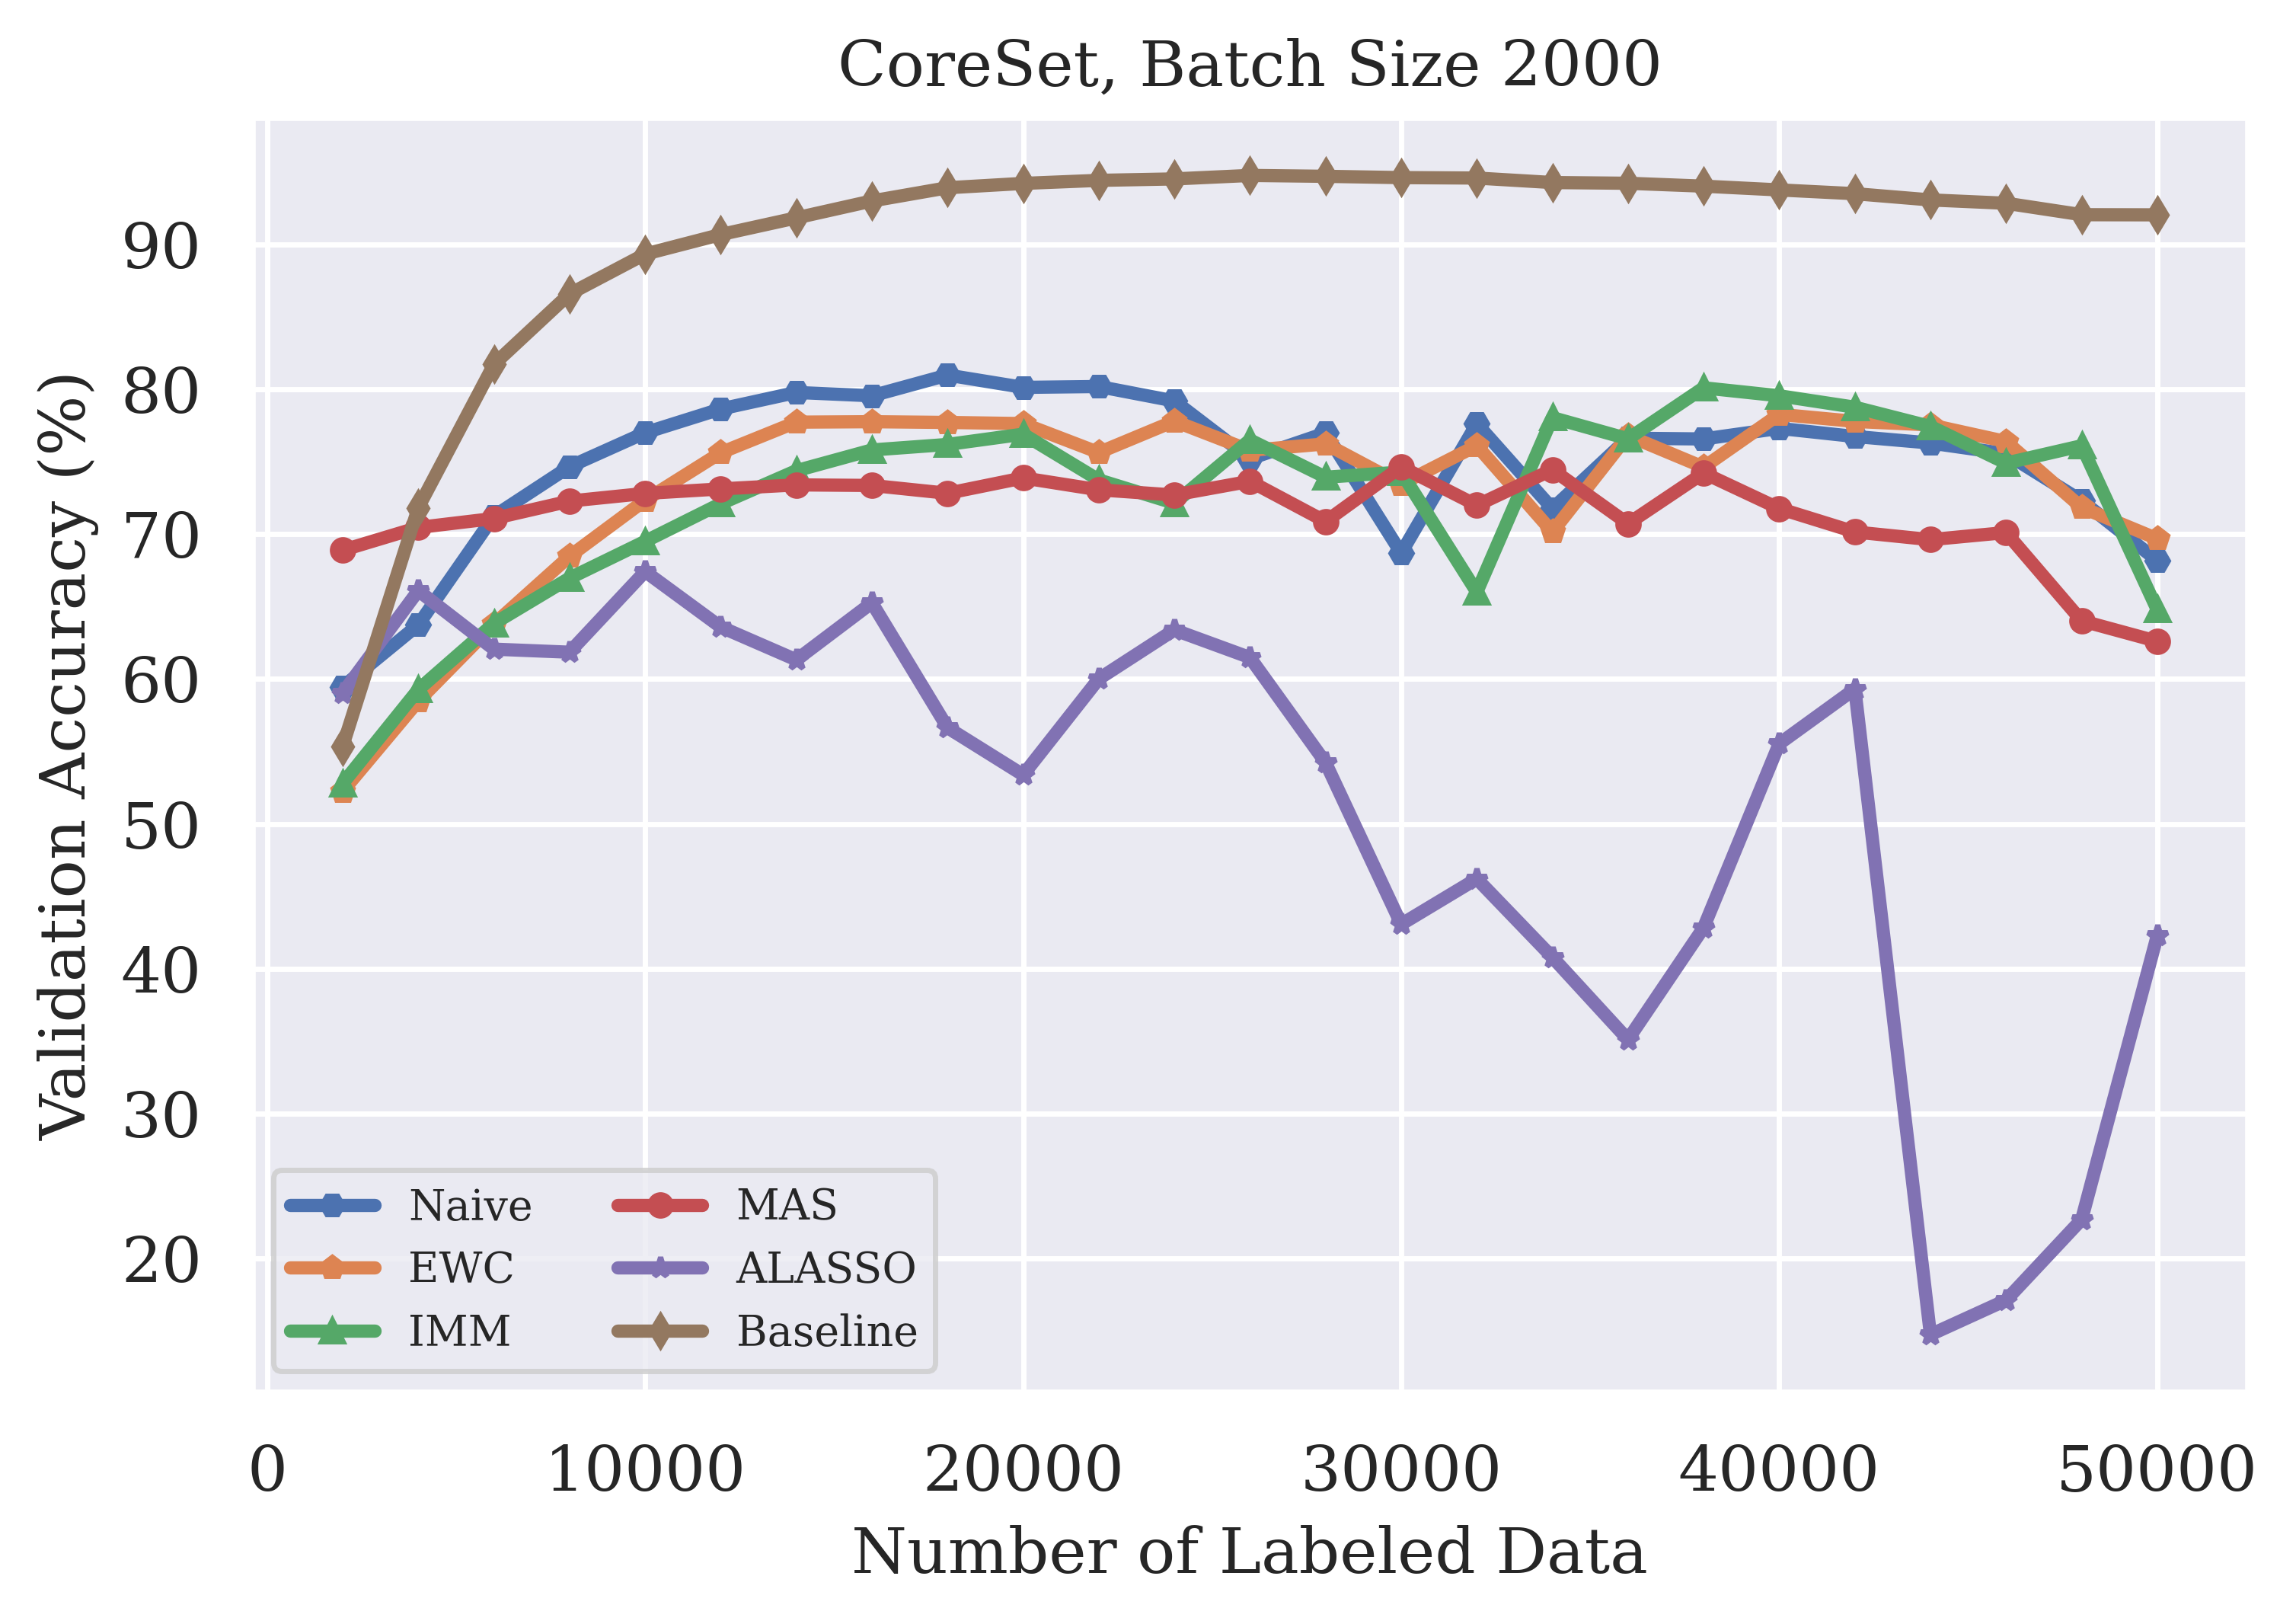
\includegraphics[width=0.32\linewidth]{images/results_CAL/coreset_2000b_acc.png} \hfill
    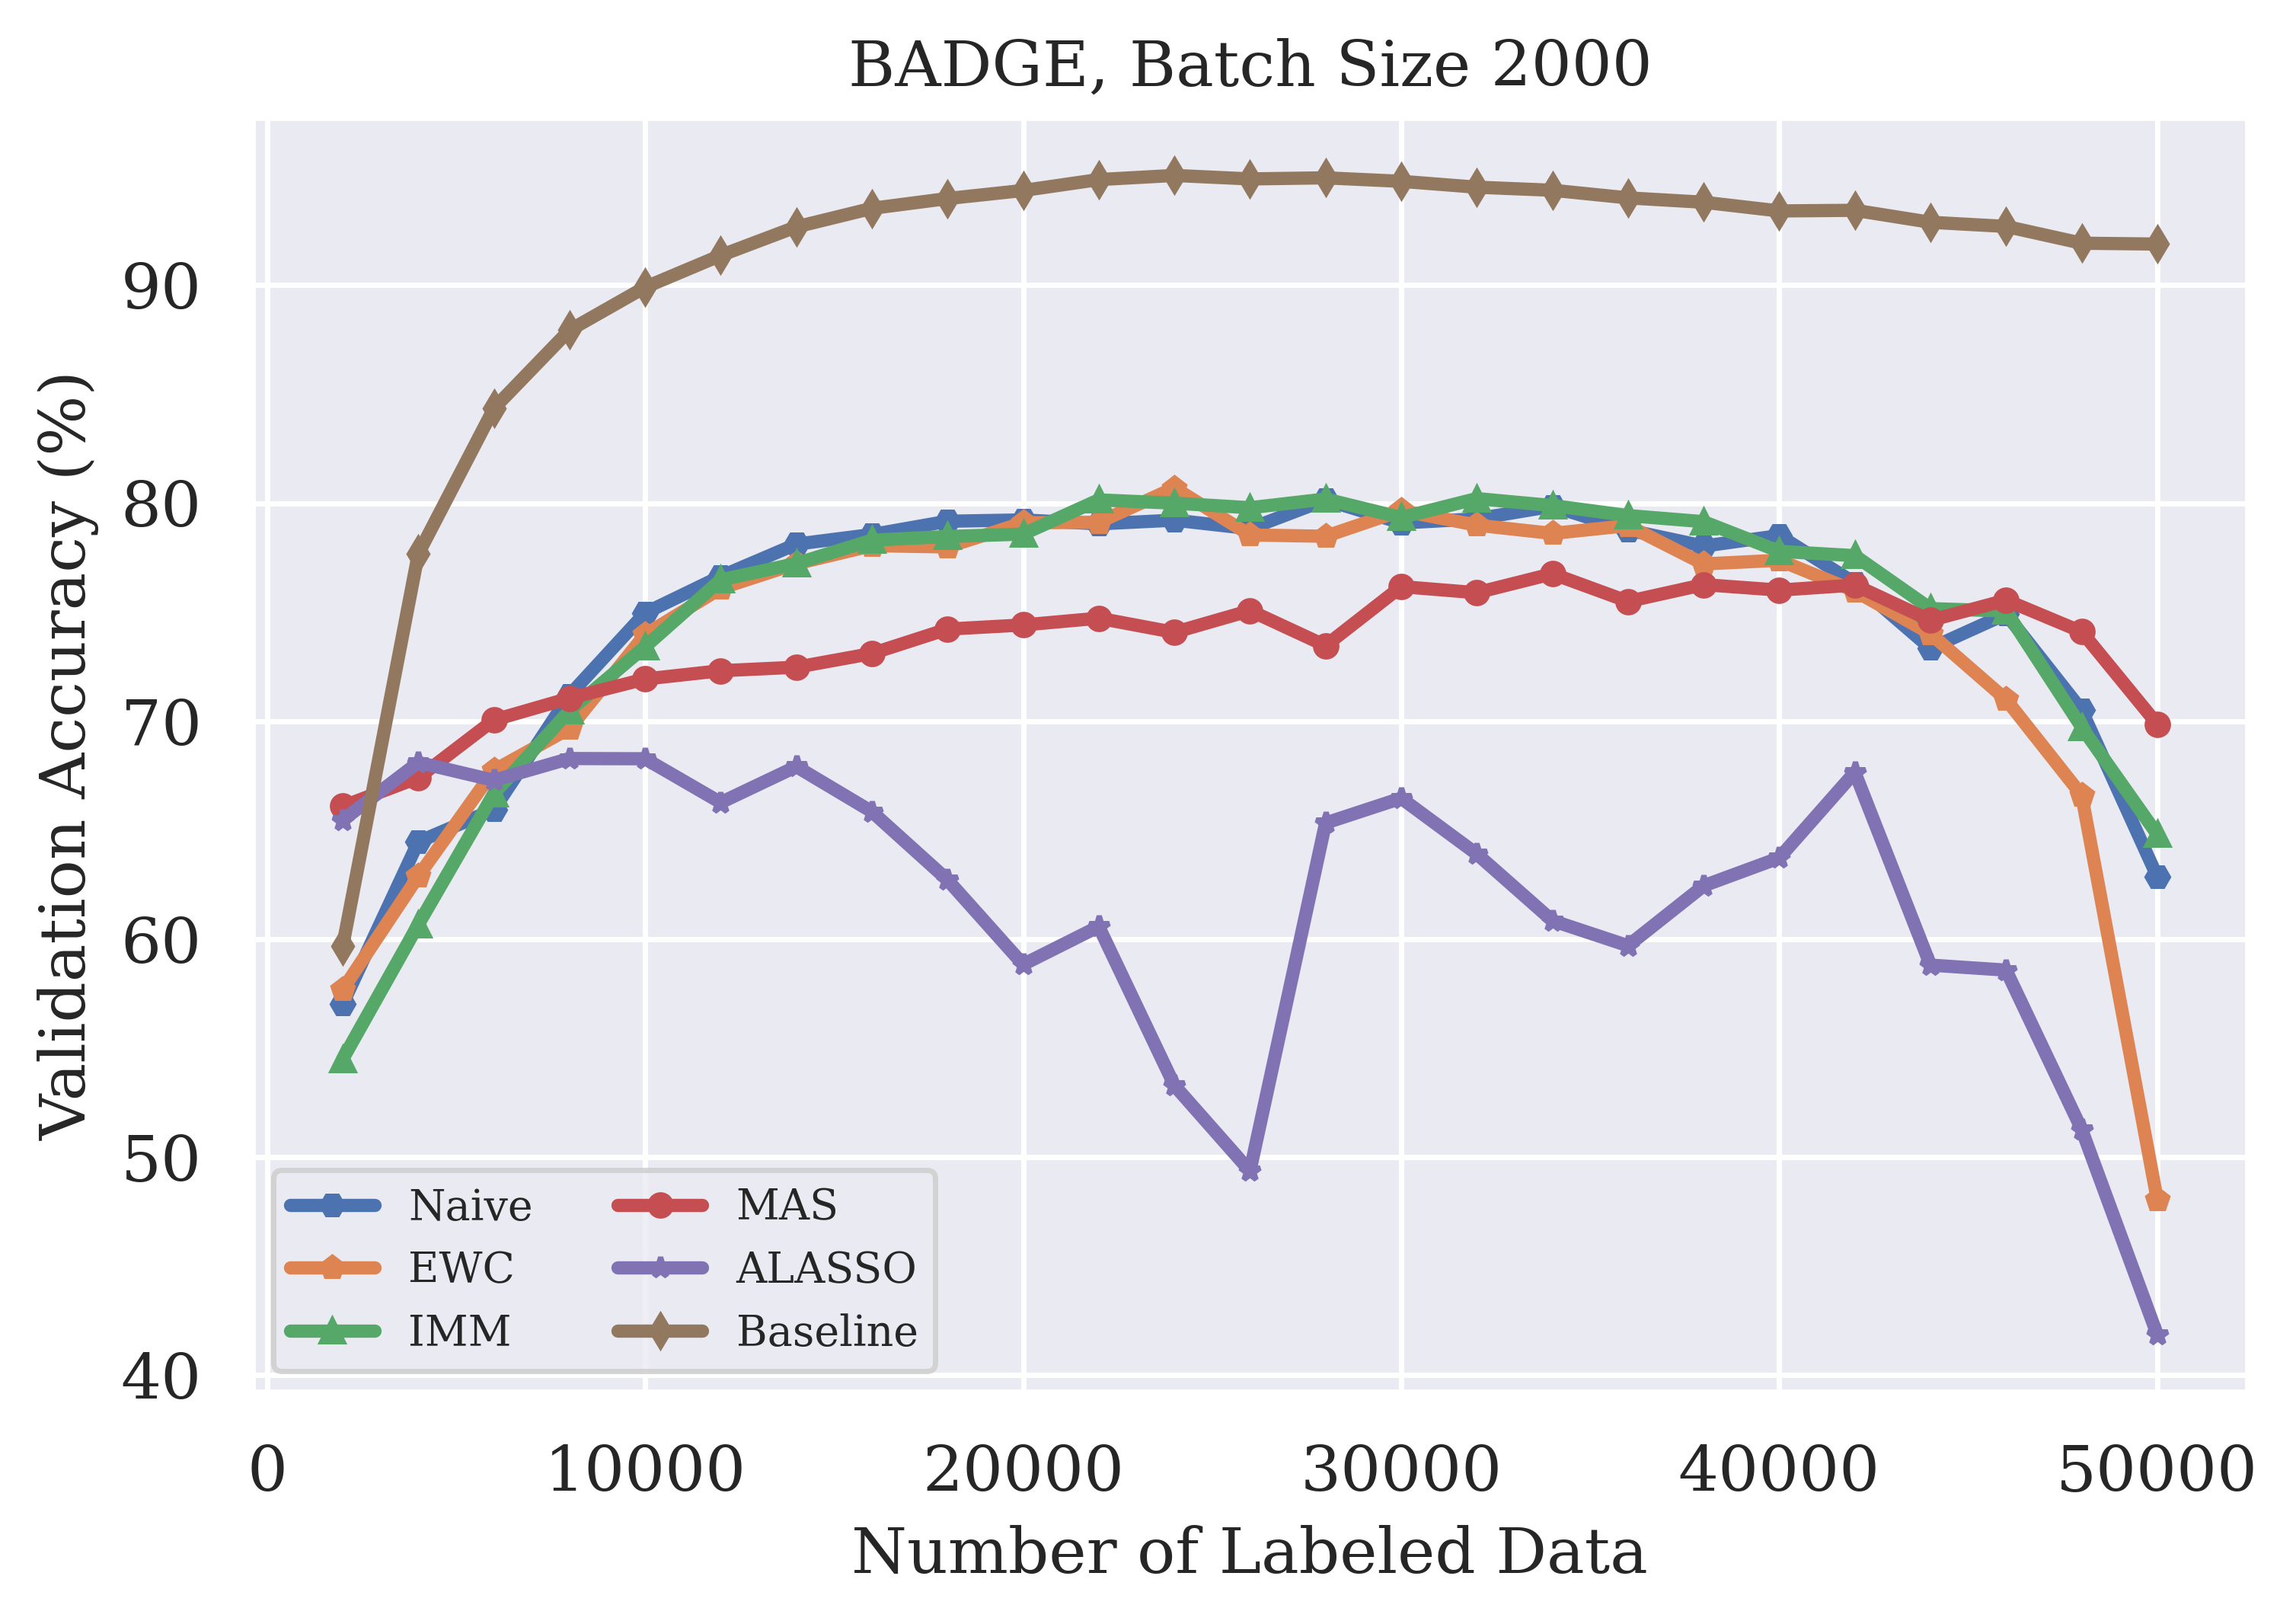
\includegraphics[width=0.32\linewidth]{images/results_CAL/badge_2000b_acc.png} \hfill
    \caption[Continual active learning with \gls{badge} with batch size 2,000]{Comparison of validation accuracy of continual active learning strategies
    with batch size 2,000.}
    \label{fig:Appendix:CAL:2000bAcc}
\end{figure}

\begin{table}[h]
    \centering
    \begin{tabular}{c | c c c c c } 
         & Random & \gls{lc} & \gls{bald} & CoreSet & \gls{badge}\\ 
        \hline 
        Baseline & 1,290 & 1,303 & 1,315 & 1,342 & 1,935 \\
        \hline
        Naive & 76 & 80 & 78 & 162 & 523 \\
        \gls{ewc} & 83 & 90 & 86 & 152 & 513\\
        \gls{imm} & 77 & 76 & 78 & 145 & 500\\
        \gls{mas} & 84 & 84 & 85 & 161 & 515\\
        \gls{alasso} & 119 & 131 & 122 & 188 & 547\\
    \end{tabular}
    \caption{Comparison of execution time of regularization-based continual learning strategies
    with batch size 2,000.}
    \label{fig:Appendix:CAL:2000bTimeTable}
\end{table}

\clearpage

\section{Model Stealing}
\label{sec:Appendix:MS}

\subsection{Evaluation of ActiveThief}
\label{sec:Appendix:MS:ActiveThief}
Because we build our continual active learning approach upon the ActiveThief framework, we believe it is important to rigorously evaluate it before we apply continual
active learning to it. In the ActiveThief paper \cite{pal2020activethief}, Pal et al. evaluate active learning for model stealing for computer vision and natural language
processing. Since this thesis focuses on computer vision tasks, we only investigate the part of the ActiveThief framework that deals with computer vision. For the ActiveThief
framework, Pal et al. introduce a proprietary thief dataset, which we dubbed Small ImageNet, and three different target model architectures, which we call ActiveThiefConv2,
ActiveThiefConv3 and ActiveThiefConv4. In the following, we evaluate the influence of the thief dataset and the target model architecture on
the success of the model stealing attack. \par
We start off by computing the validation accuracies of the ActiveThiefConv model family, which the ActiveThief framework and ours use as target and substitute models. 
These numbers have not been given by the authors of ActiveThief in their paper. However, we believe they are crucial to understanding the performance of the ActiveThief framework
and our continual active learning approach. Each model of the ActiveThiefConv family is trained on MNIST and CIFAR-10. Additionally, we train ActiveThiefConv3 on CIFAR-100,
because we will conduct experiments with CIFAR-100 in section \ref{sec:Evaluation:MS}. We omit the results for ActiveThiefConv2 and ActiveThiefConv4 on CIFAR-100
because they are not relevant to this thesis. The results are depicted in table \ref{fig:TargetModelAccuracies}. They show that ActiveThiefConv4, the most complex model,
achieves the highest validation accuracy on both MNIST and CIFAR-10. While the validation accuracy for MNIST is above 98 \% for all models, there is a difference in validation
accuracy of almost 20 percentage points between ActiveThiefConv2 and ActiveThiefConv4 on CIFAR-10. This shows that the complexity of the target model architecture has a
significant influence on validation accuracy. \par

\begin{table}[h]
    \centering
    \begin{tabular}{c| c c c} 
        & ActiveThiefConv2 & ActiveThiefConv3 & ActiveThiefConv4 \\ 
        \hline 
        MNIST & 98.42 & 98.91 & 99.01 \\
        CIFAR-10 & 66.61 & 80.67 & 84.47 \\
        CIFAR-100 & - & 42.90 & - \\
    \end{tabular}
    \caption{Validation accuracies (in \%) of our target model architectures on MNIST, CIFAR-10 and CIFAR-100.}
    \label{fig:TargetModelAccuracies}
\end{table}

Next, we evaluate the influence of the target model architecture and substitute model architecture on the success of the model stealing attack. We use the ActiveThiefConv model
family as target and substitute models and perform one model stealing attack for each combination of target and substitute model. We use the active learning strategy CoreSet
with a batch size of 1,000 and a total budget of 20,000 to perform the attacks. The results are depicted in figure \ref{fig:CIFAR10modelComp}. The plots in the figure represent
the progression of agreement between the target and substitute model on the validation set of the CIFAR-10 dataset at the end of each experiment. Overall, we observe that the
agreement between the target and substitute model is highest when we use a target model of low complexity (i.e., ActiveThiefConv2) and a substitute model of moderate to high
complexity (i.e., ActiveThiefConv3 and ActiveThiefConv4). This is in line with the results of the ActiveThief paper \cite{pal2020activethief}. However, we report the accuracy
after a budget of 20,000, whereas Pal et al. presumably report the accuracy after training on the full thief dataset. To further study the behavior of model stealing attacks
using different model architectures, we conduct the same experiment using MNIST as the target model dataset. The results of this experiment can be found in figure 
\ref{fig:MNISTmodelComp}. Overall, the results are similar to those on CIFAR-10. However, it is evident that the discrepancies between
the target and substitute model combinations are larger. \par

\begin{figure}[!htb]
    \centering
    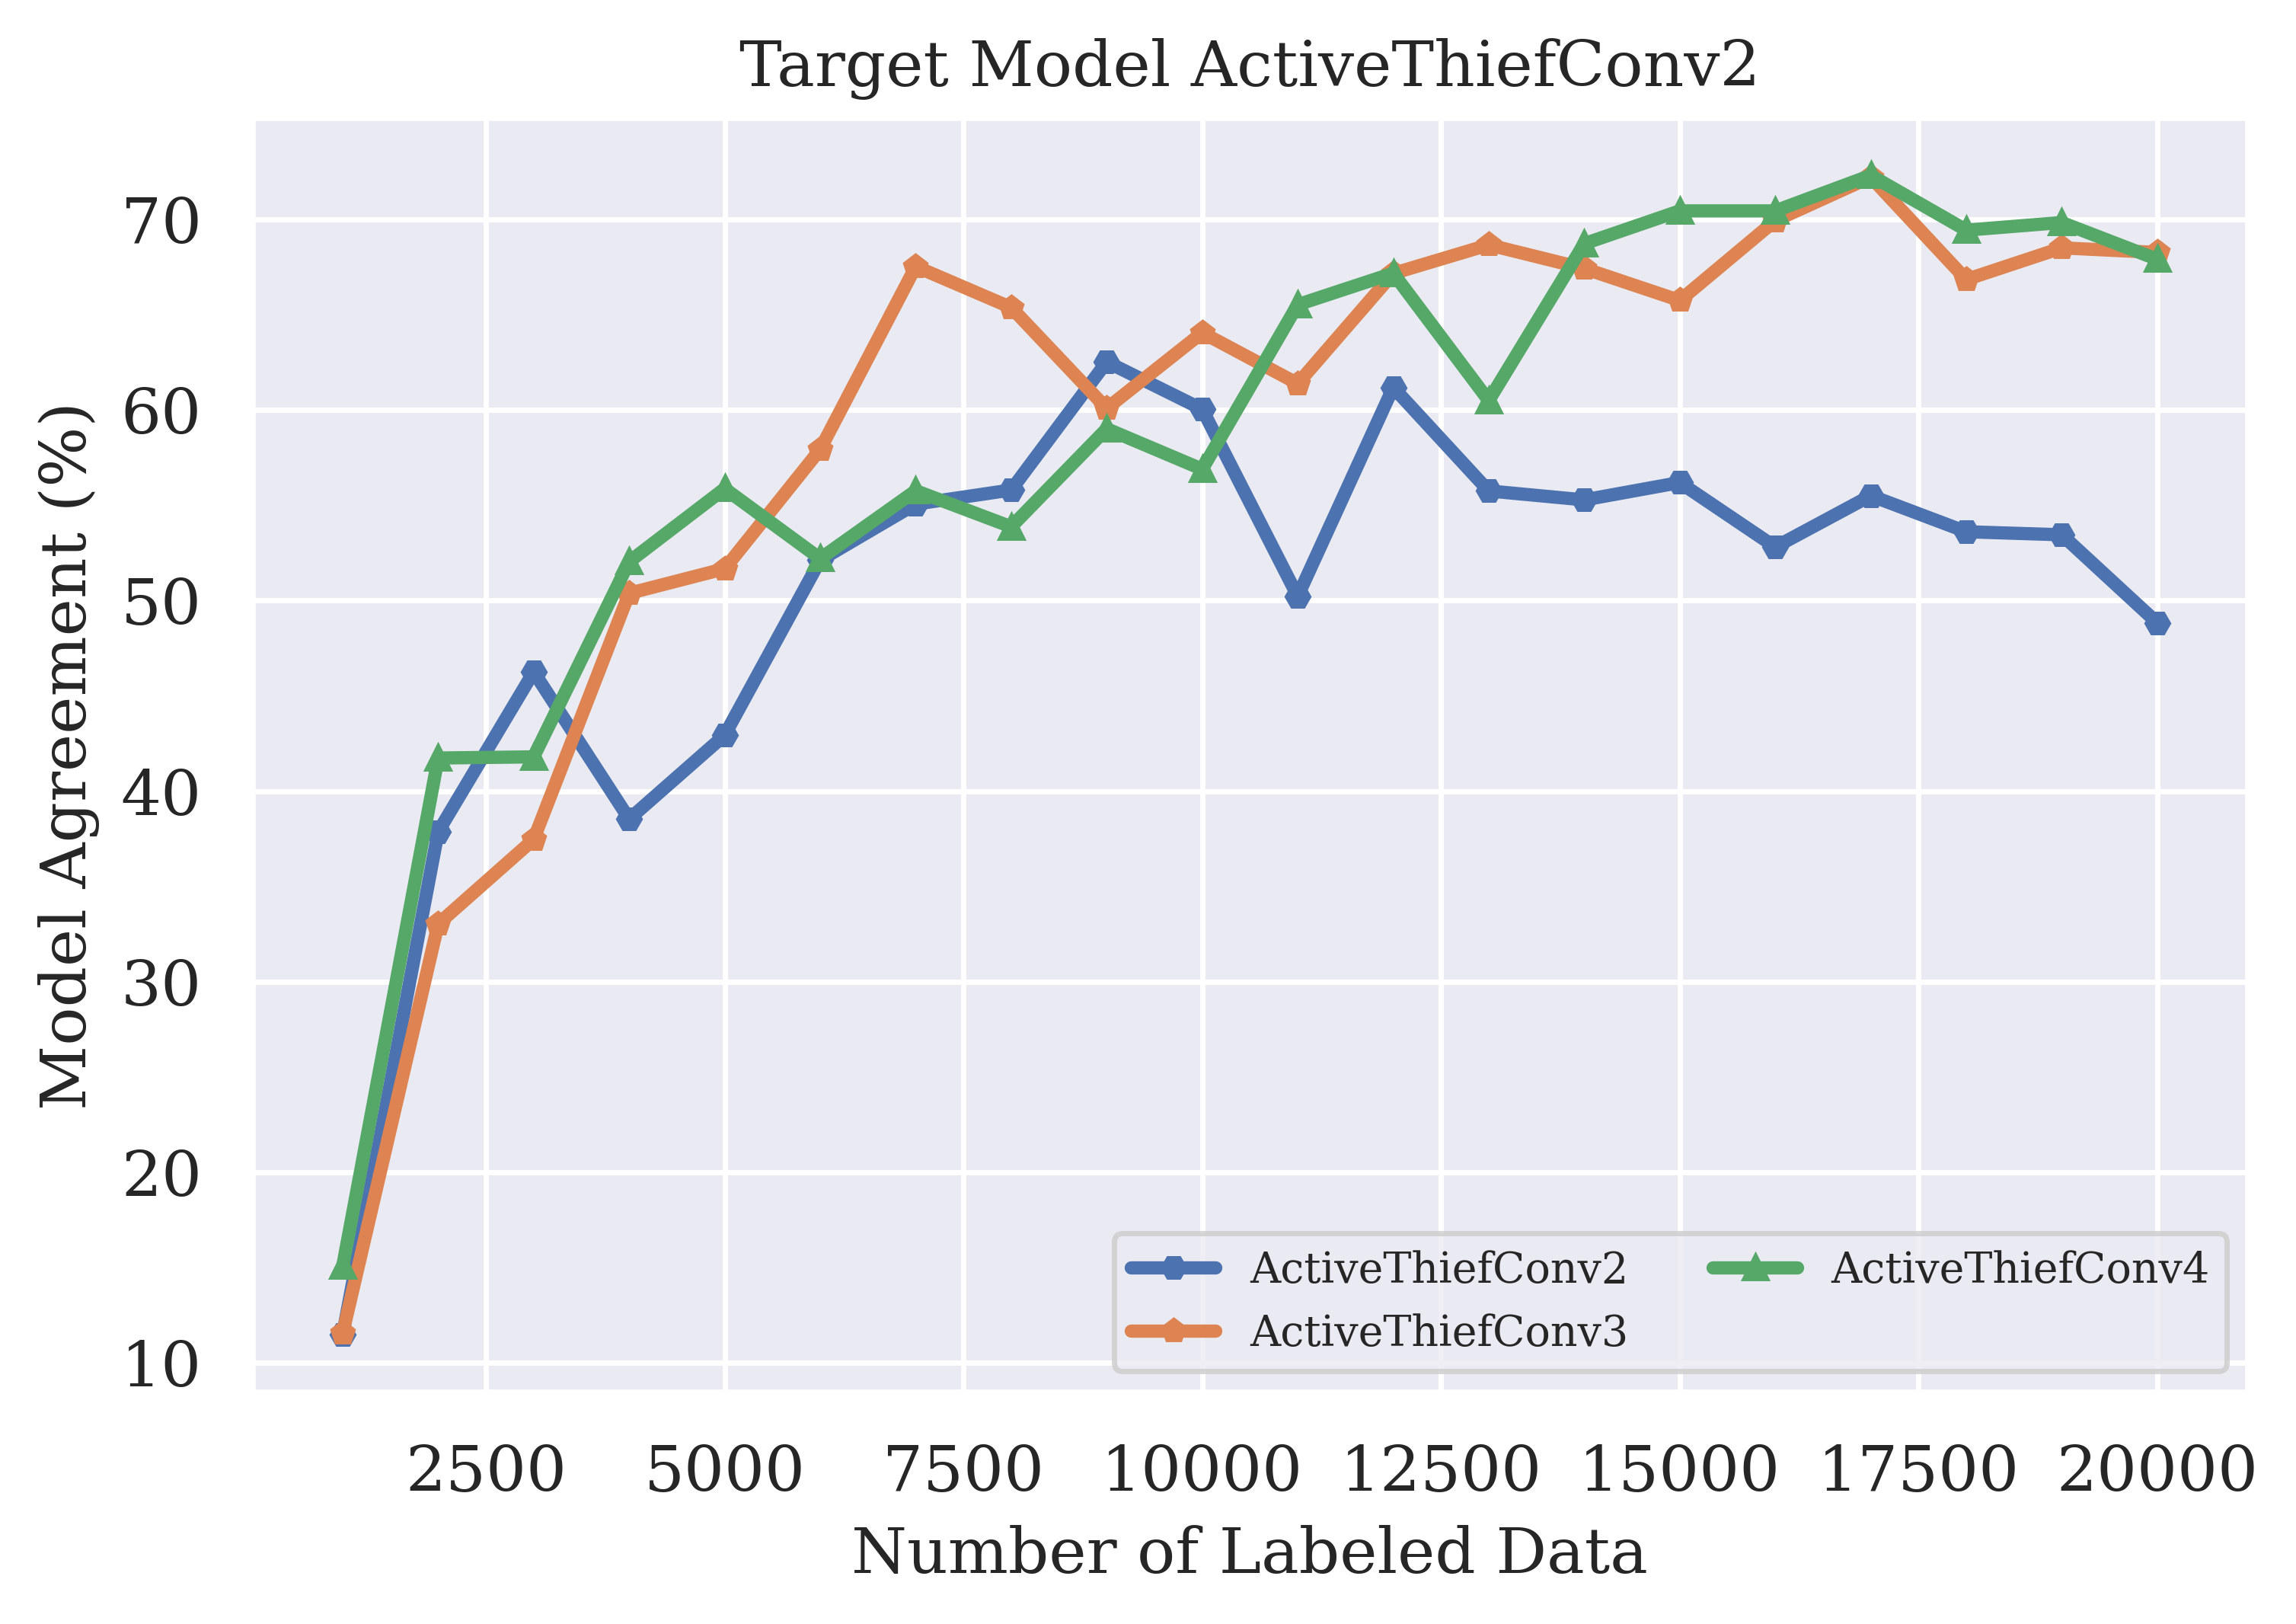
\includegraphics[width=0.32\linewidth]{images/MSInsights/mnist_act2.png} \hfill
    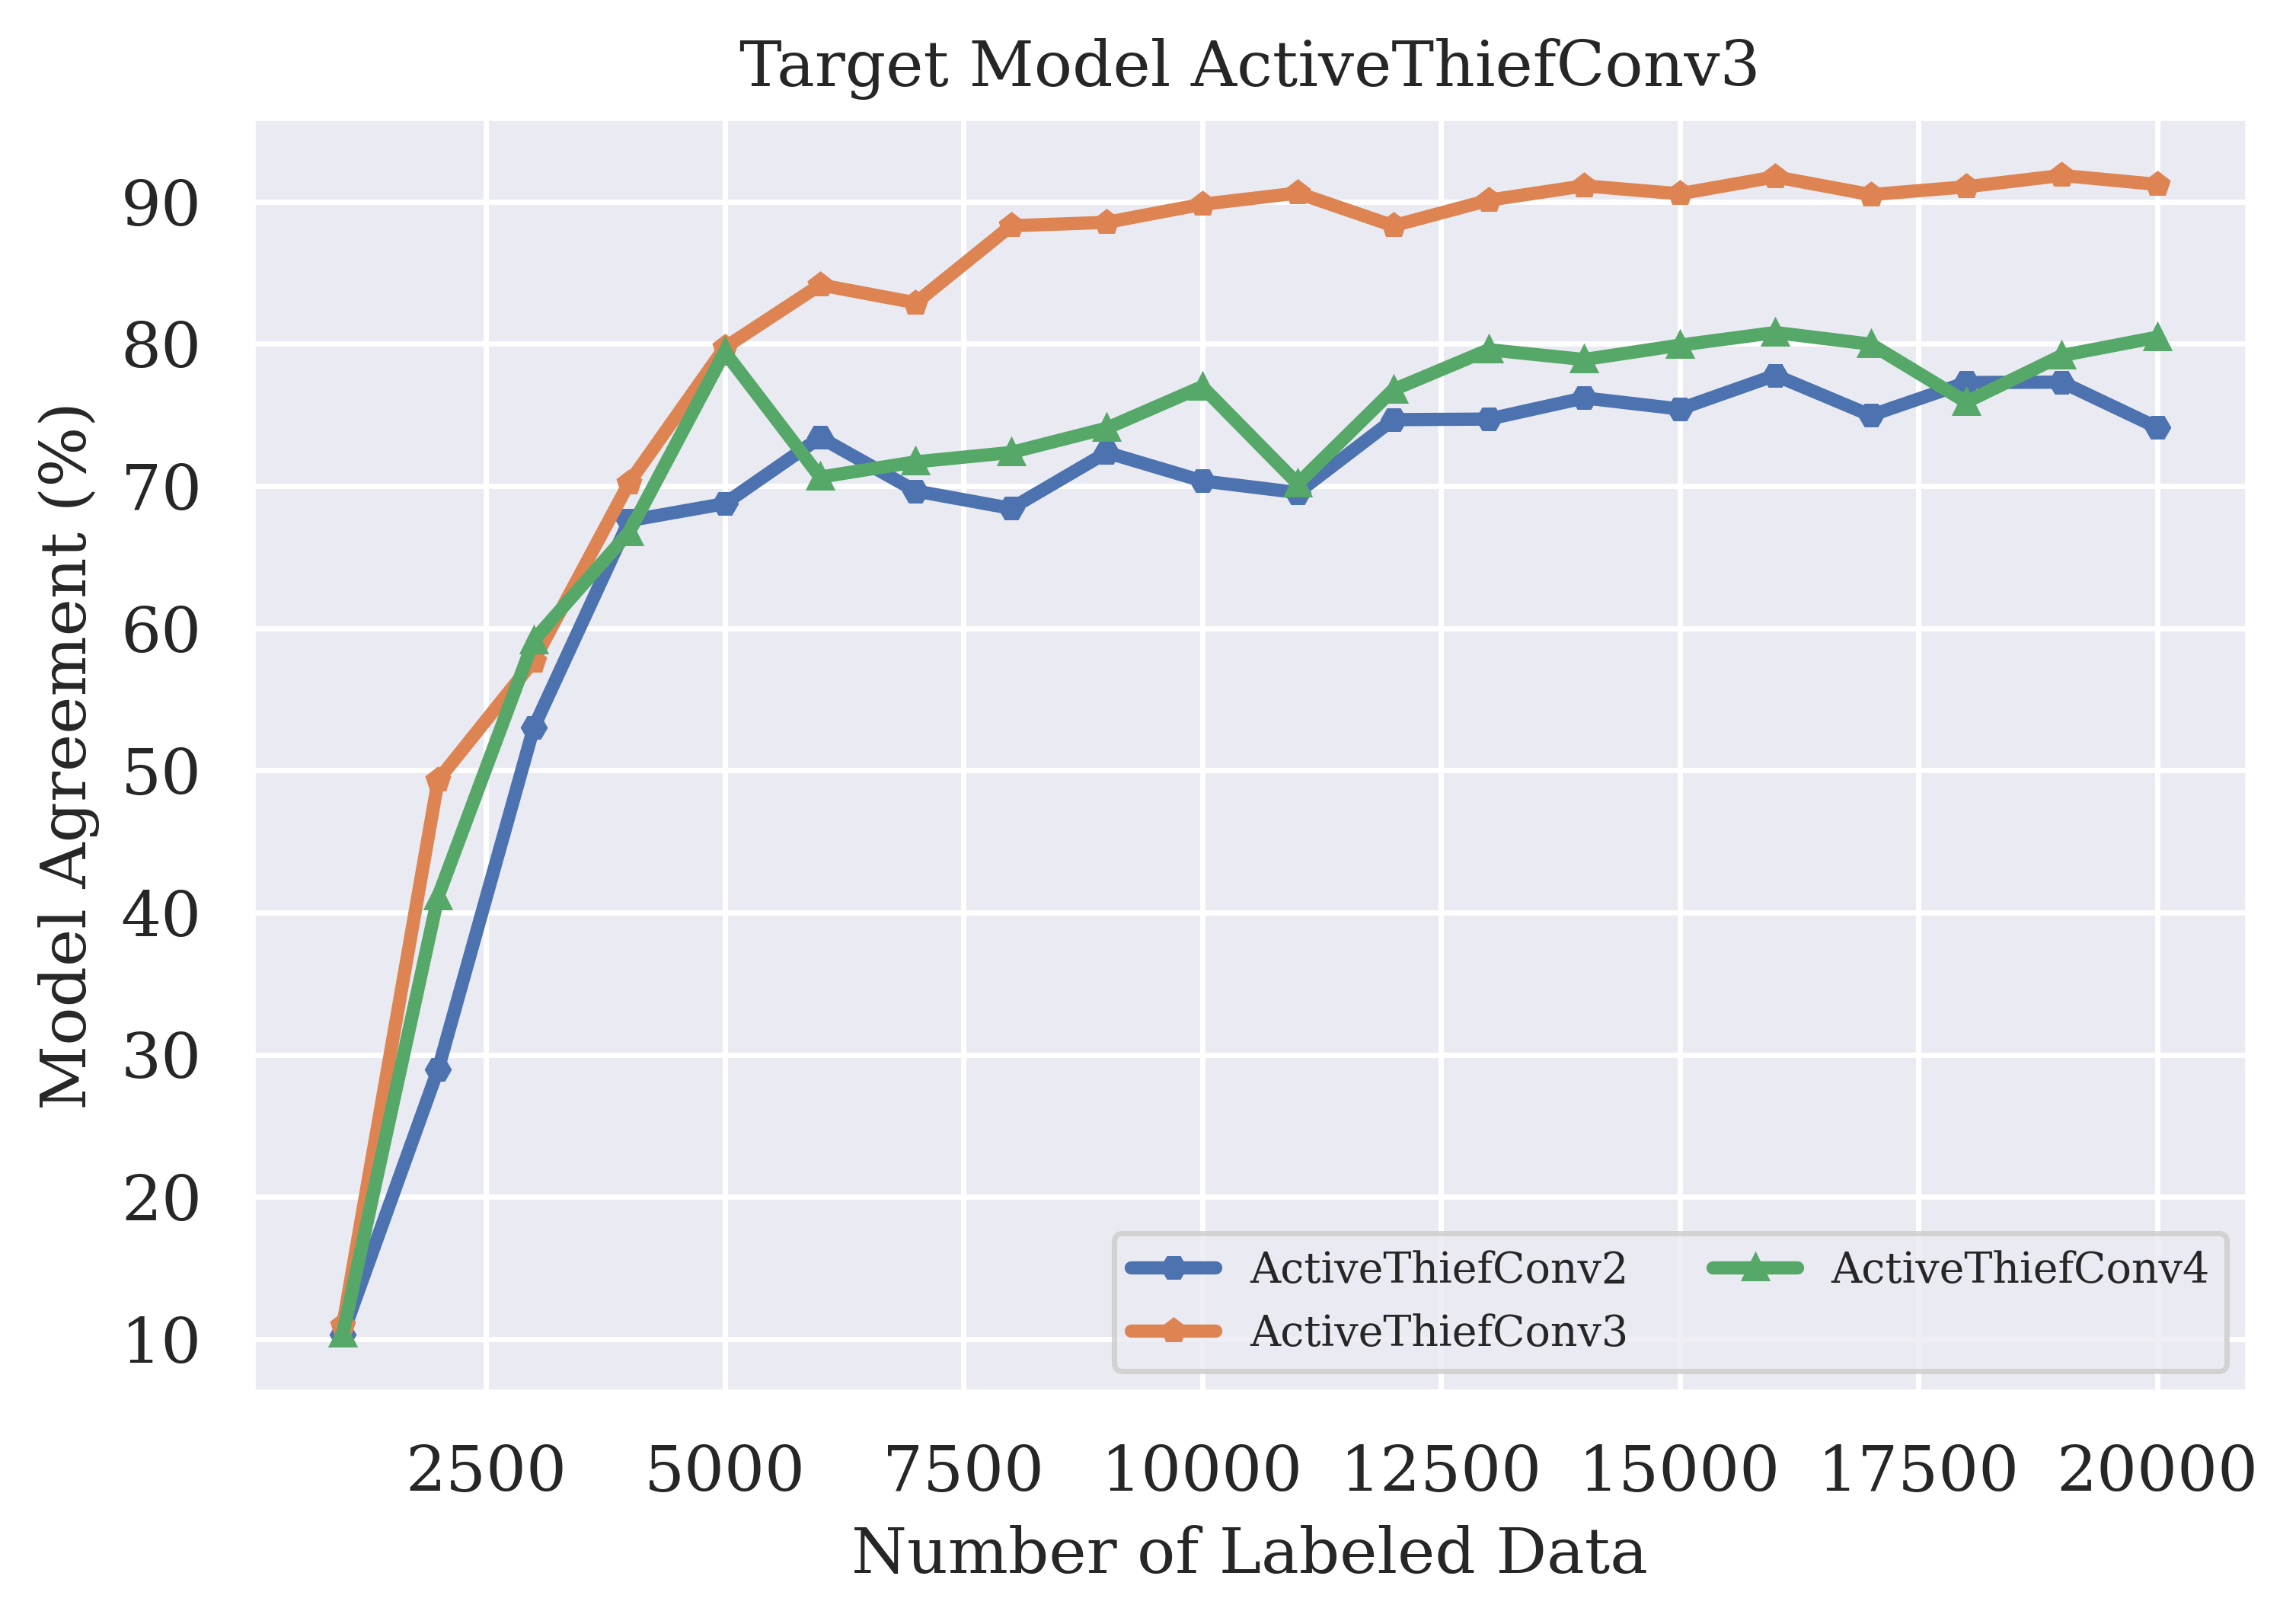
\includegraphics[width=0.32\linewidth]{images/MSInsights/mnist_act3.png} \hfill
    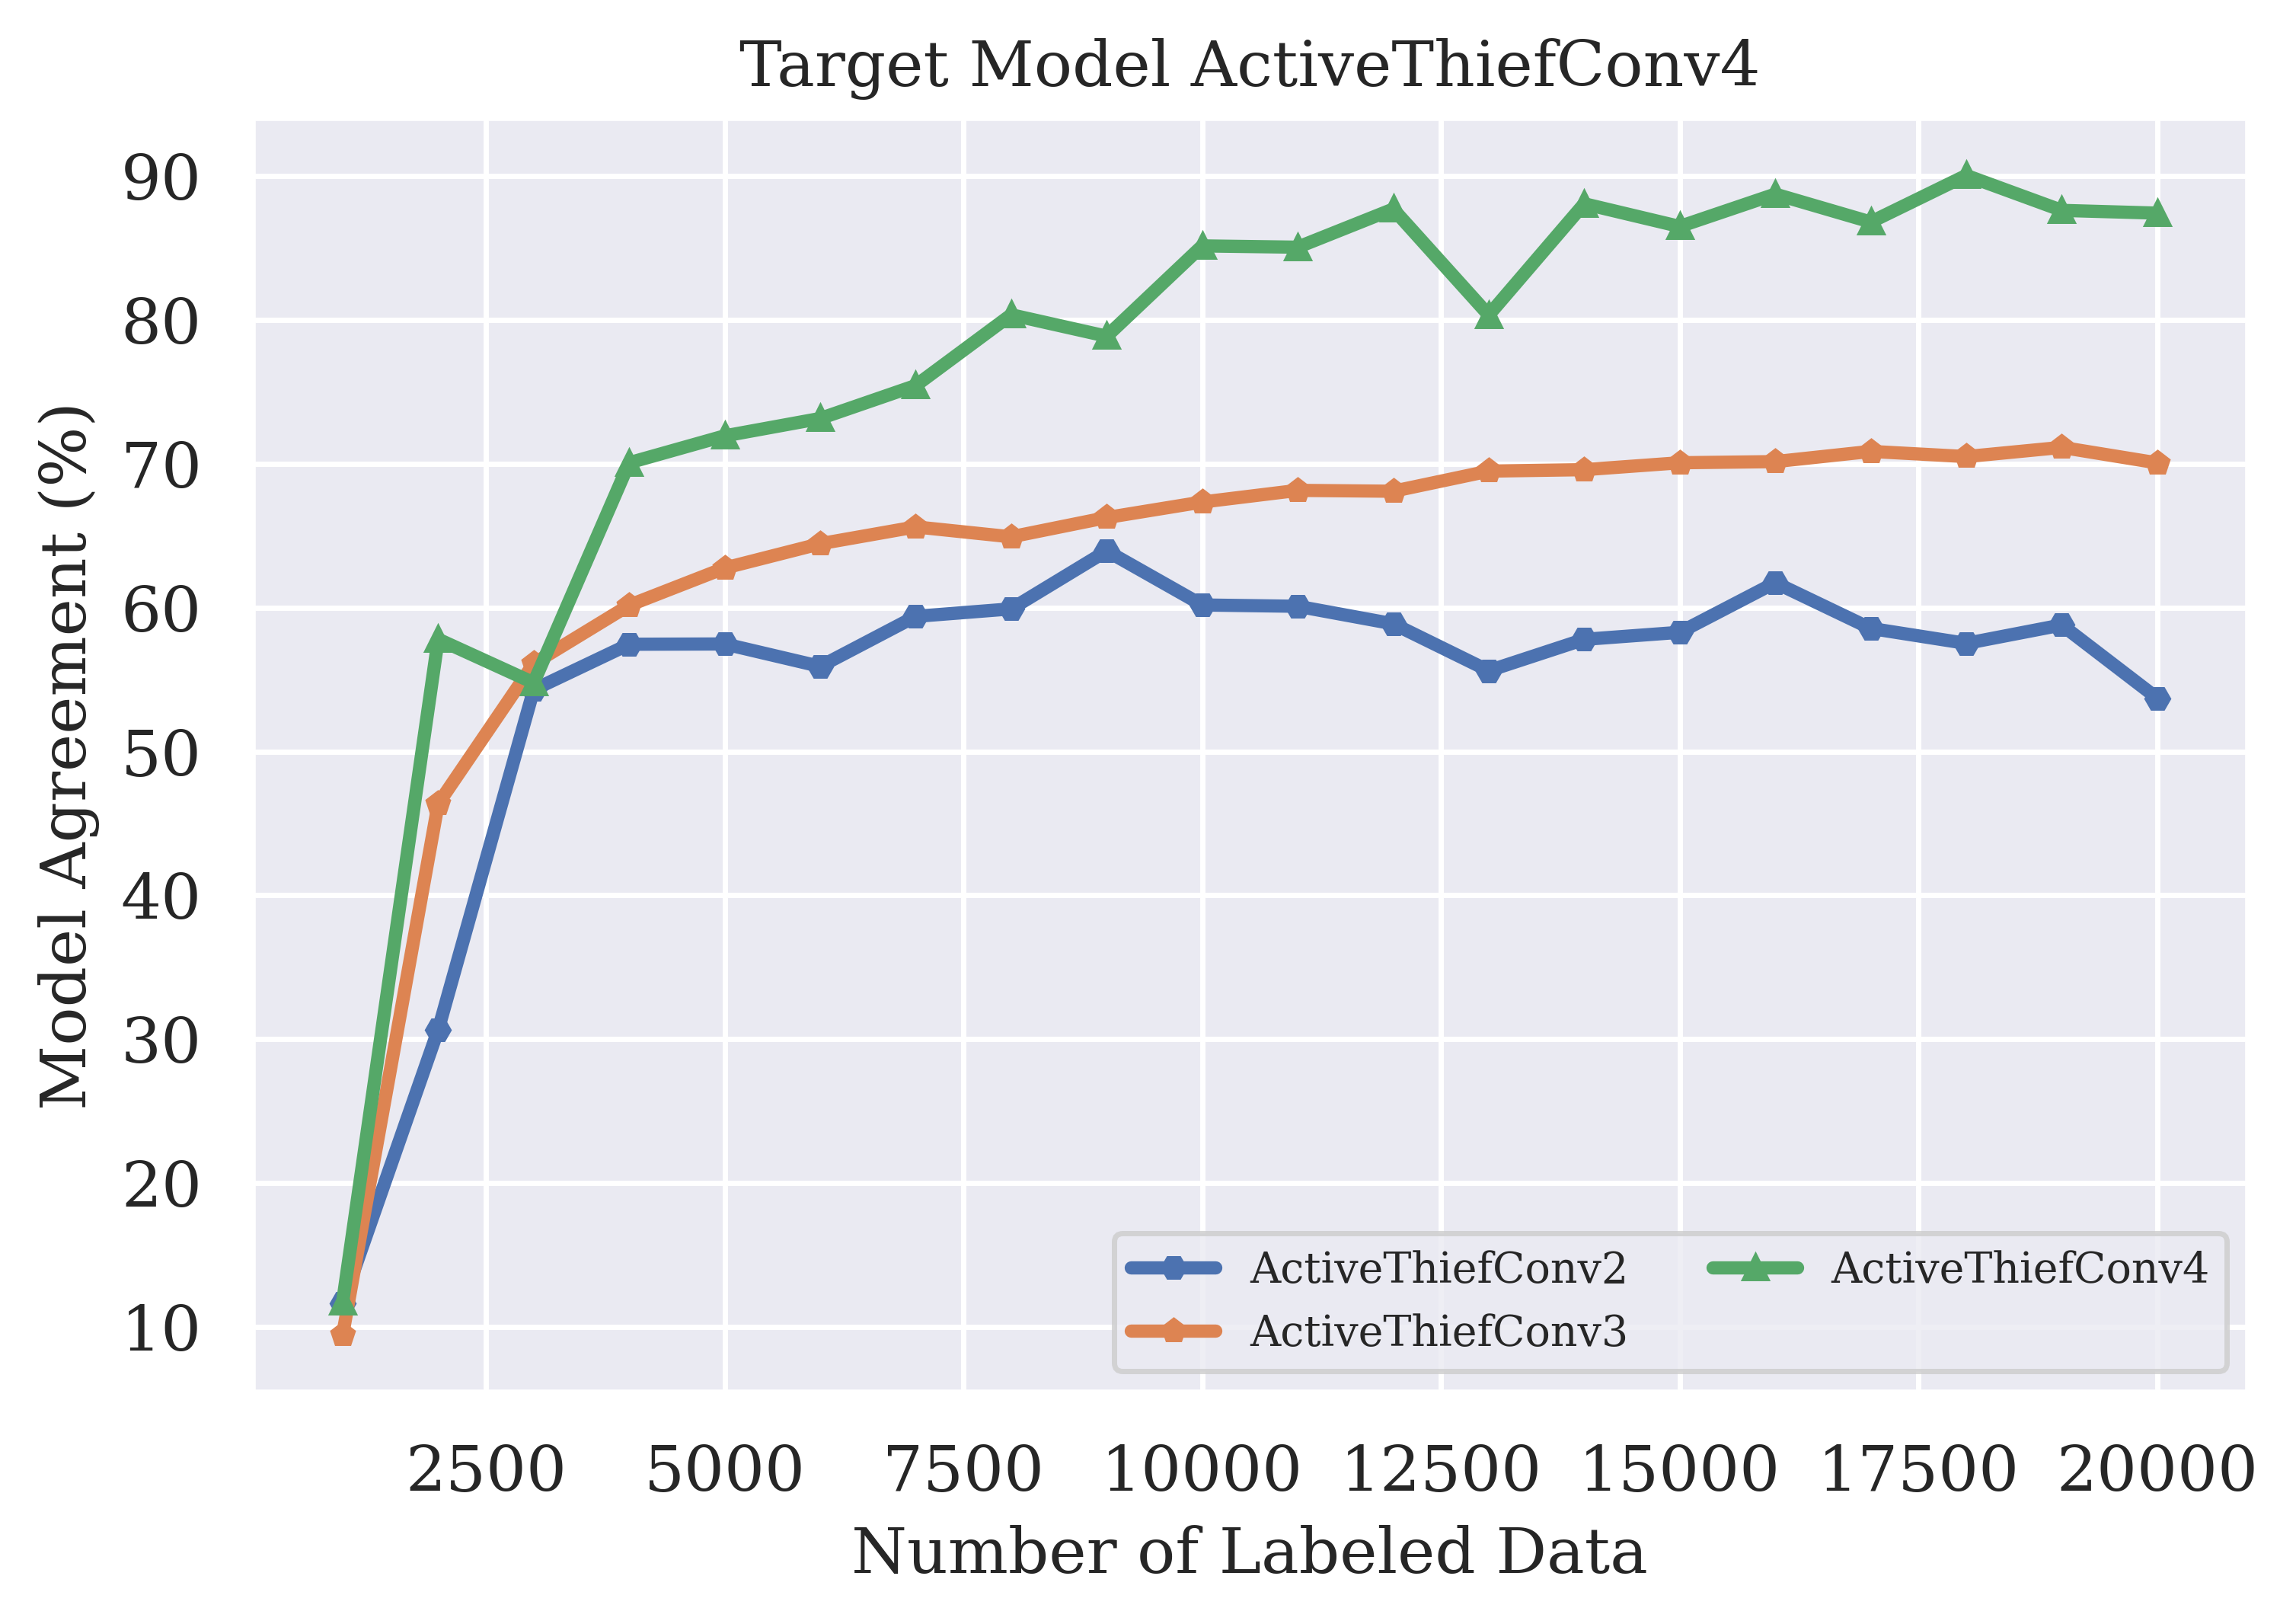
\includegraphics[width=0.32\linewidth]{images/MSInsights/mnist_act4.png}
    \caption{Agreement progression with varying model architectures on MNIST.}
    \label{fig:MNISTmodelComp}
\end{figure}

\begin{figure}[!htb]
    \centering
    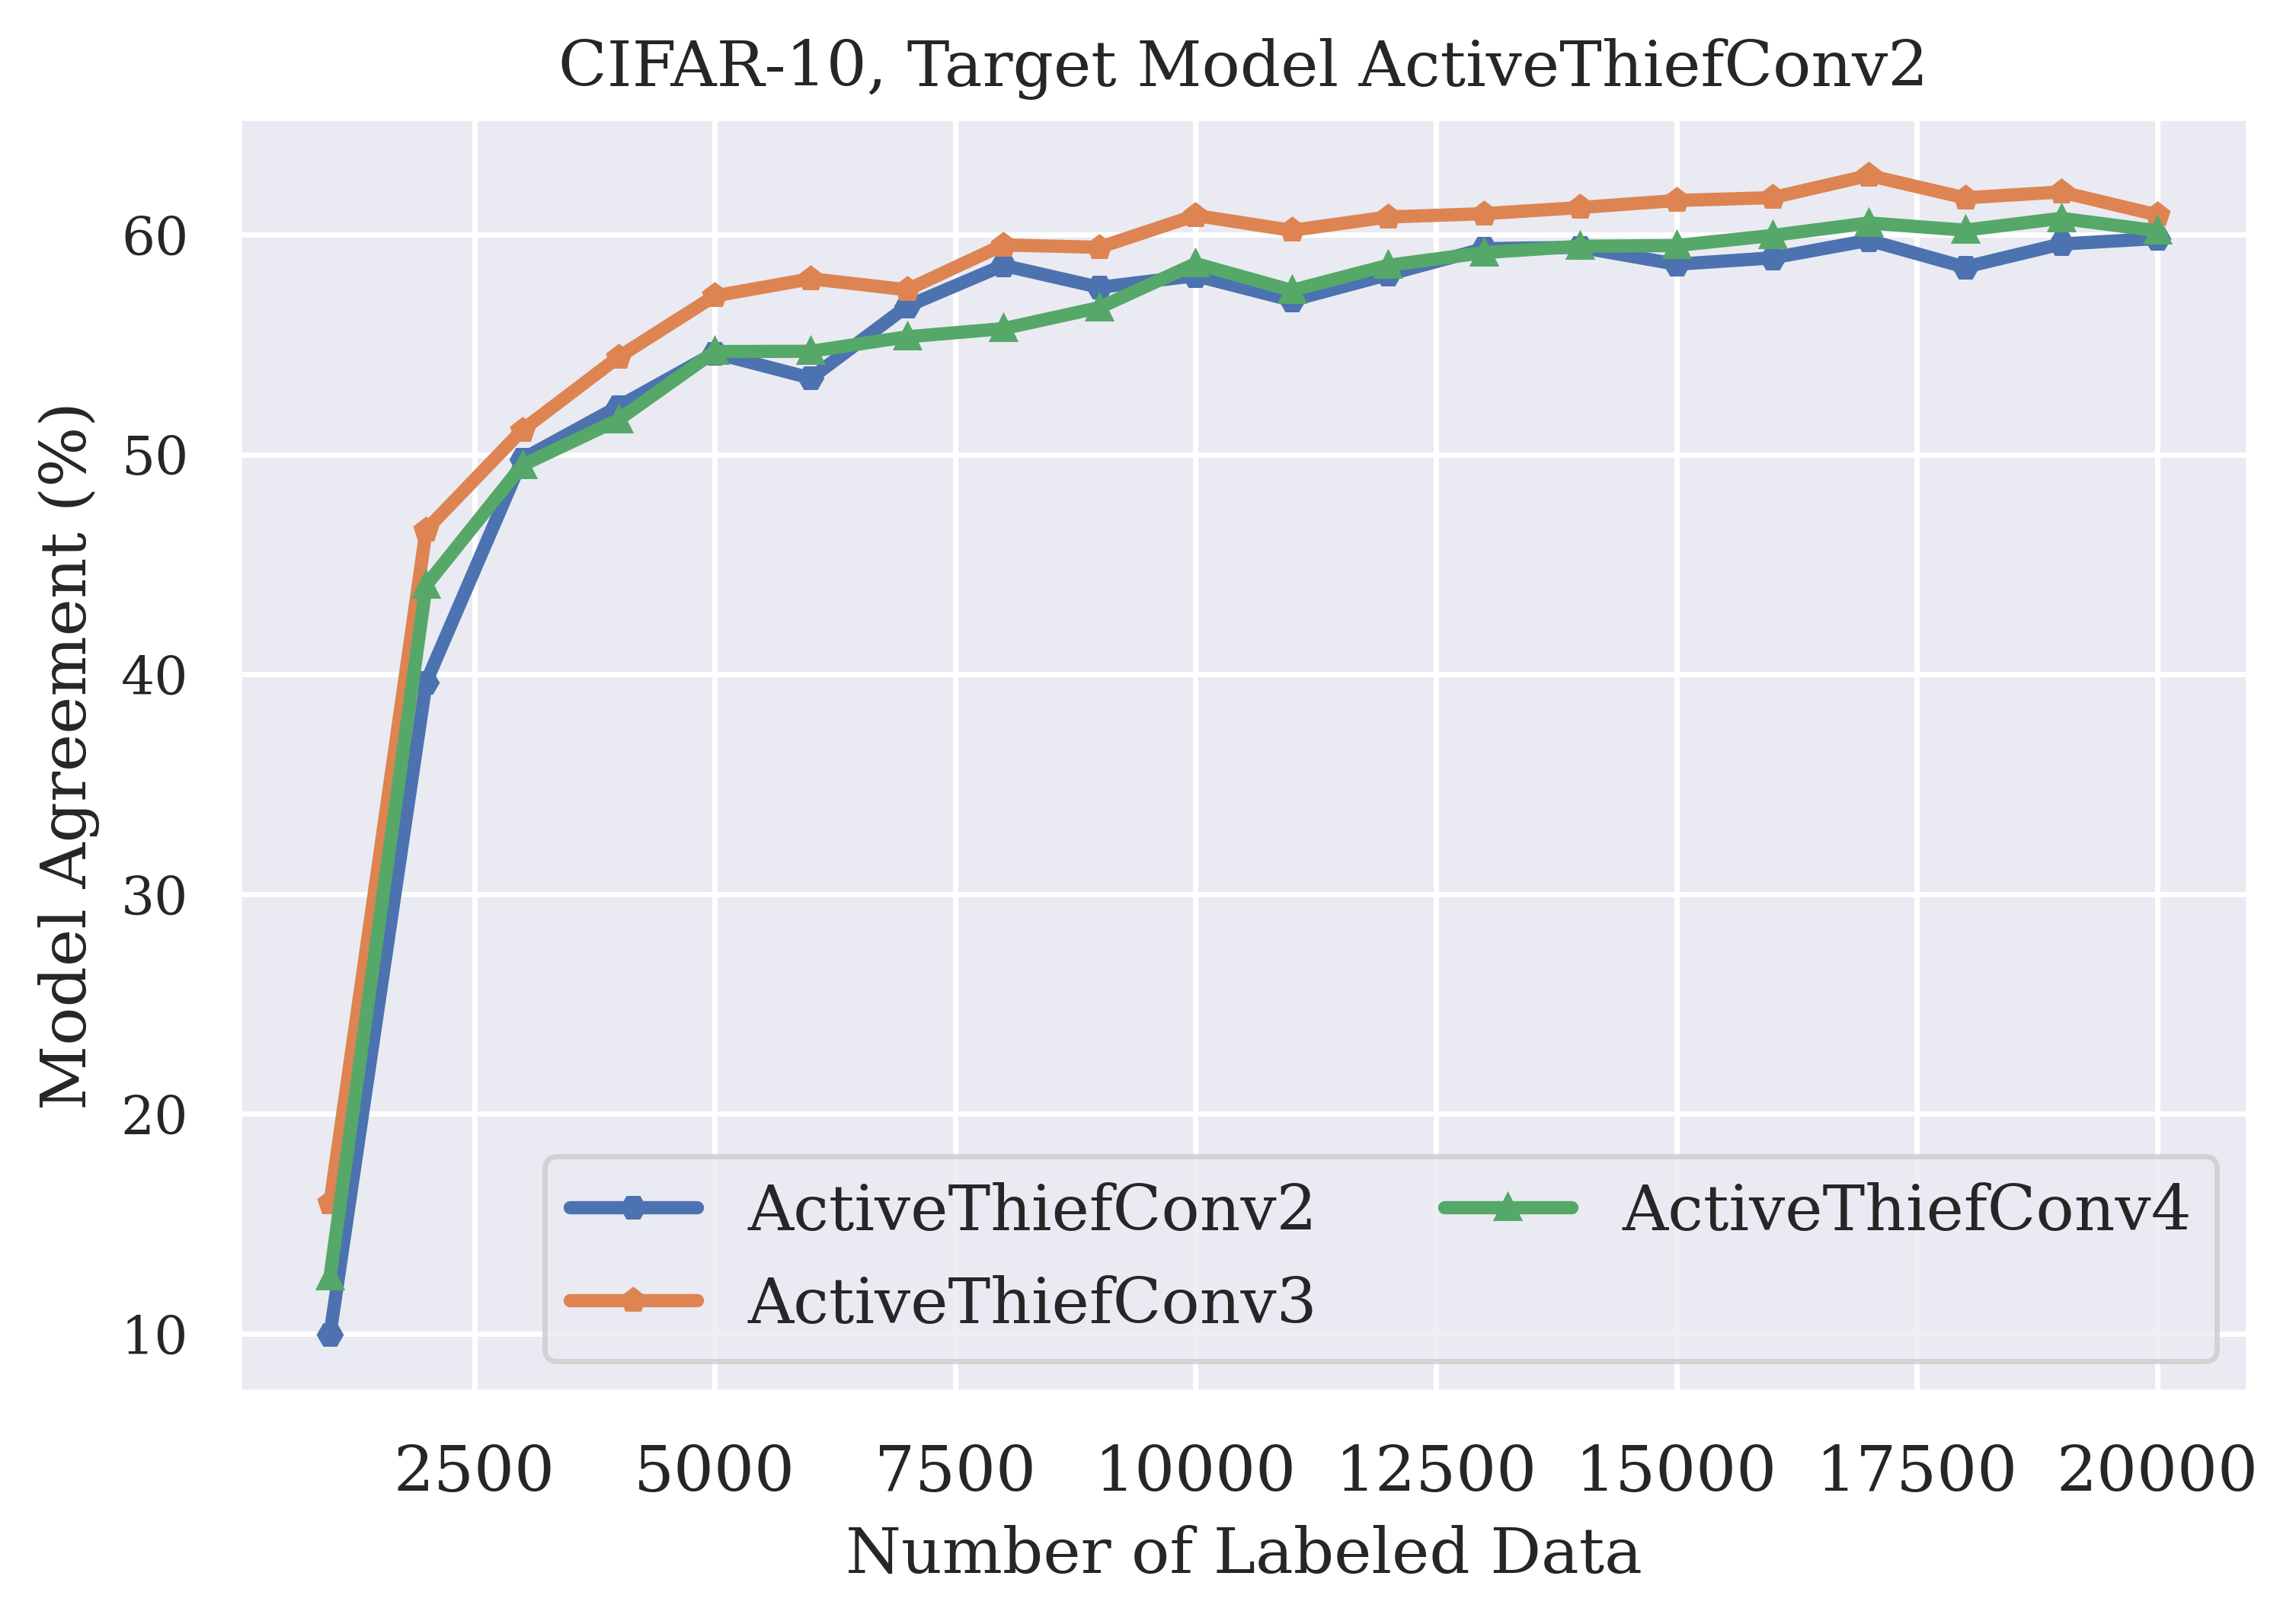
\includegraphics[width=0.32\linewidth]{images/MSInsights/cifar_act2.png} \hfill
    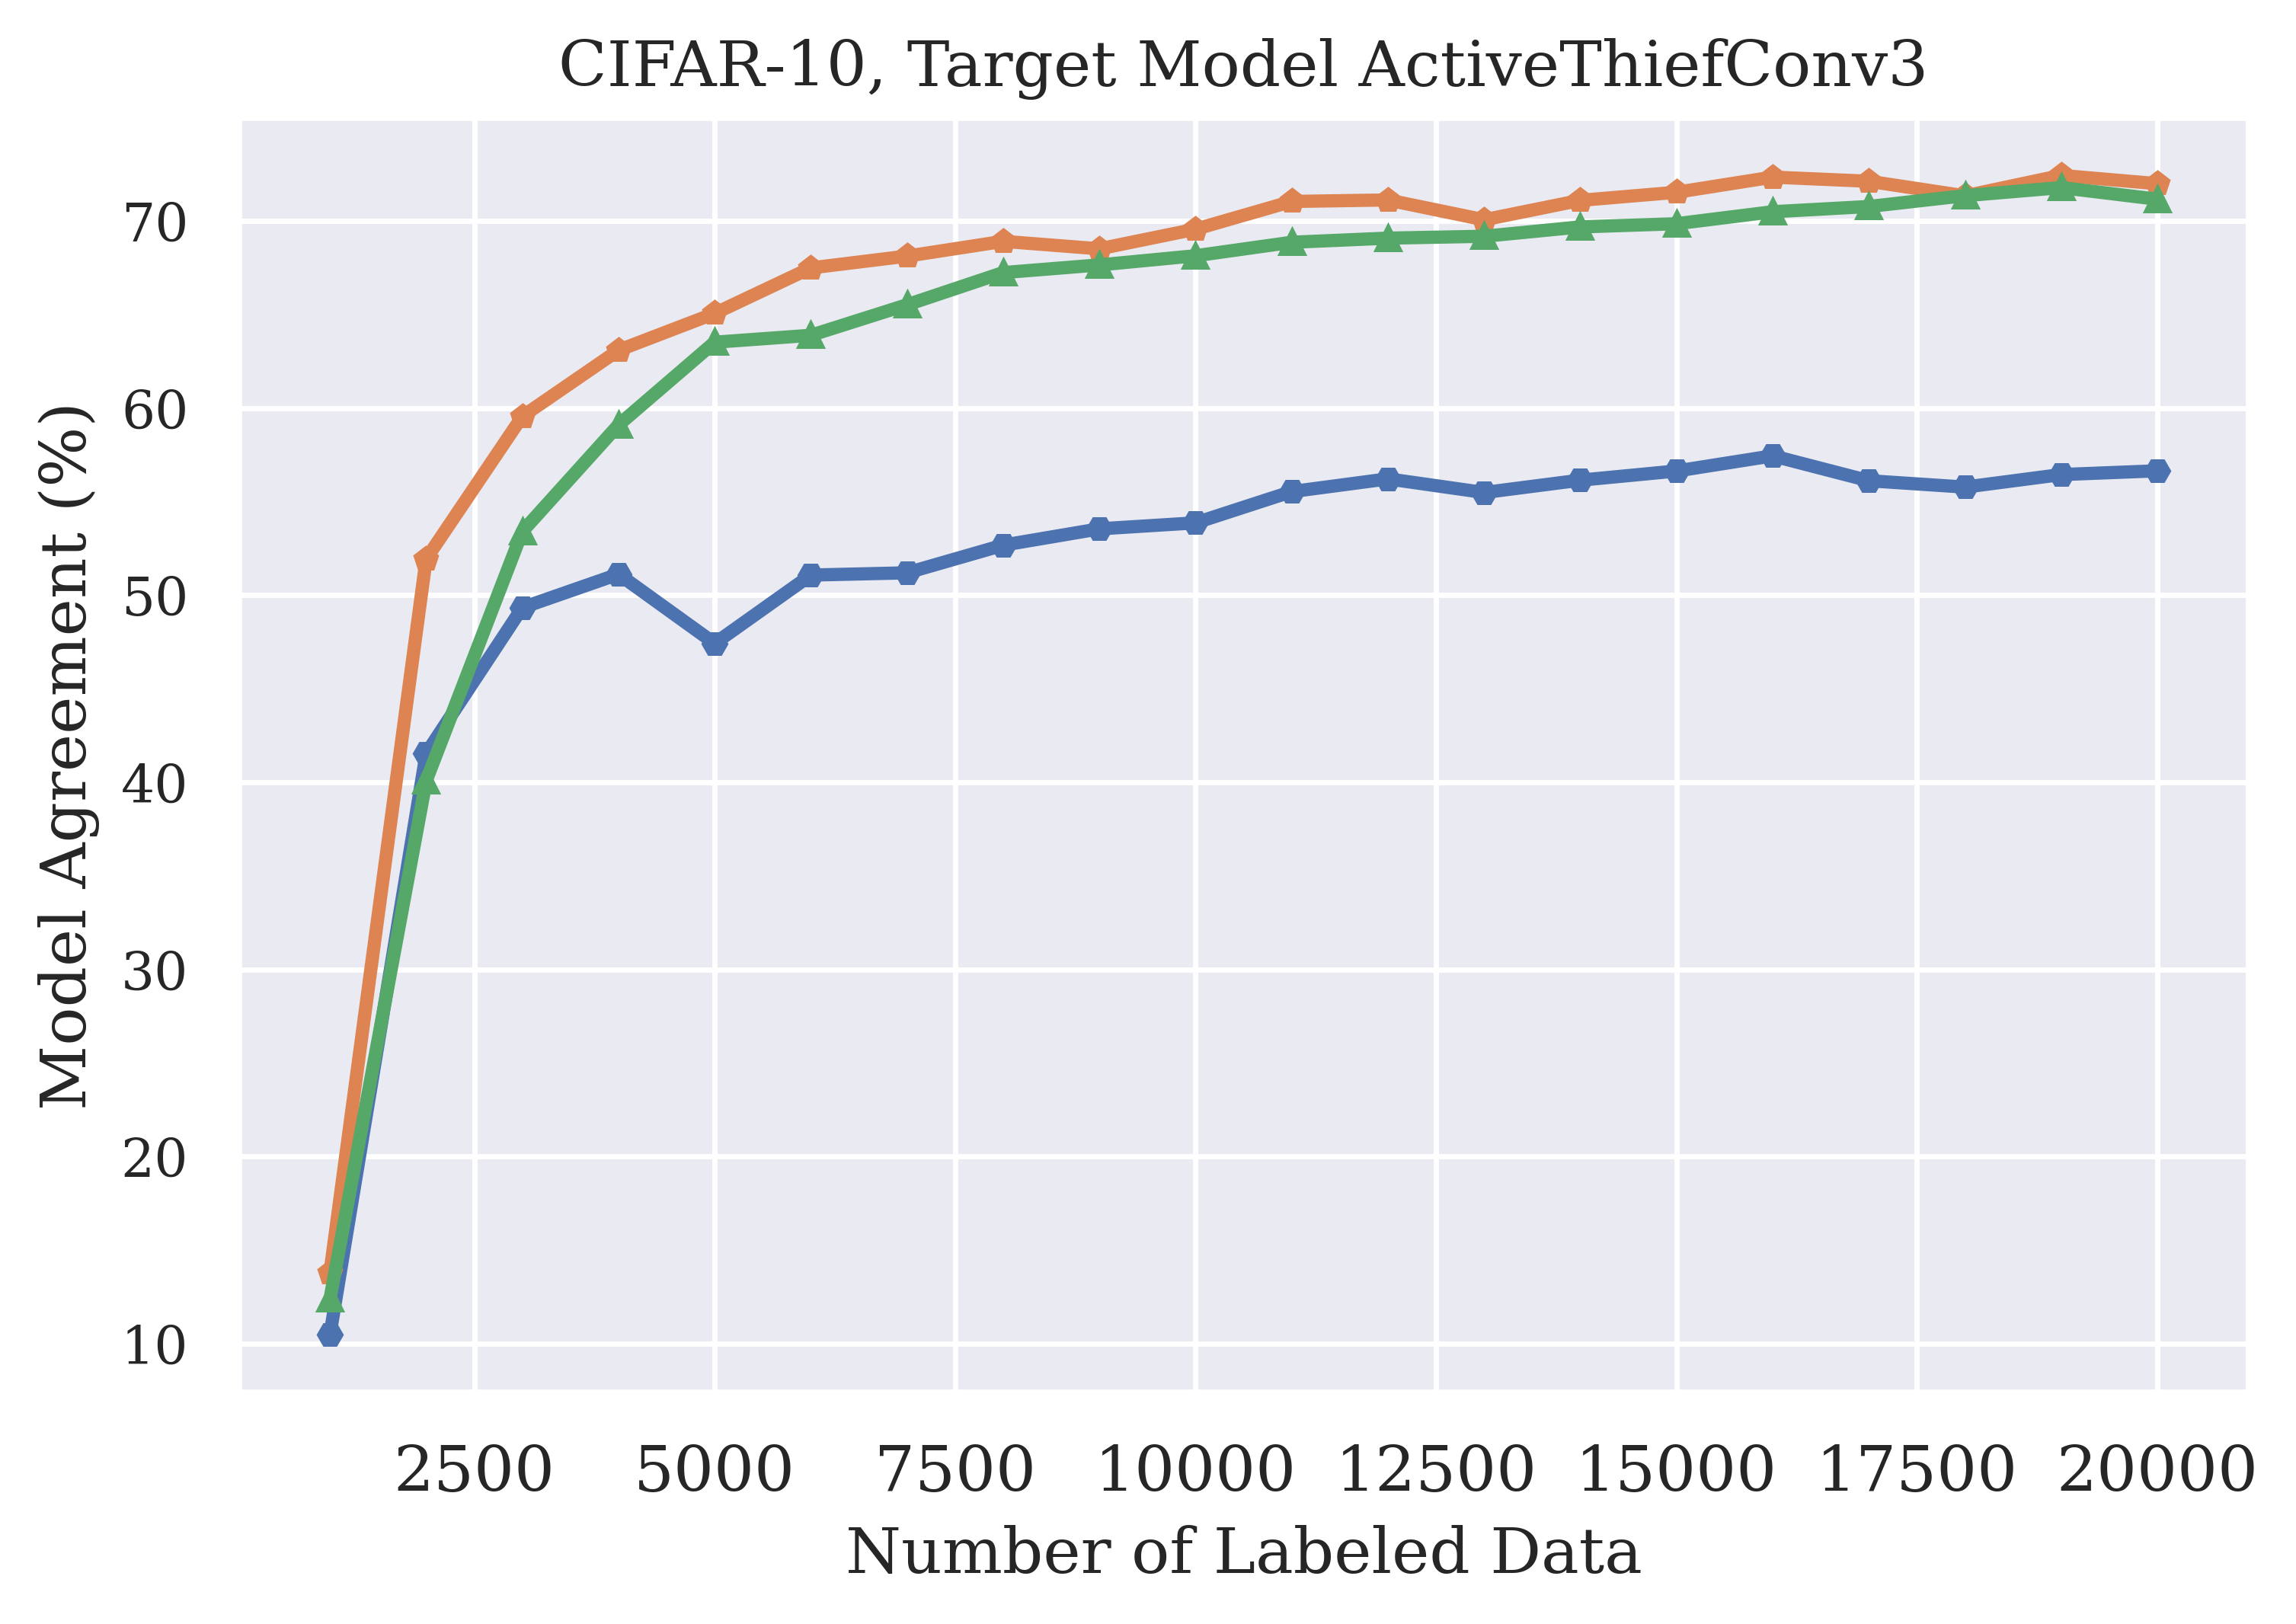
\includegraphics[width=0.32\linewidth]{images/MSInsights/cifar_act3.png} \hfill
    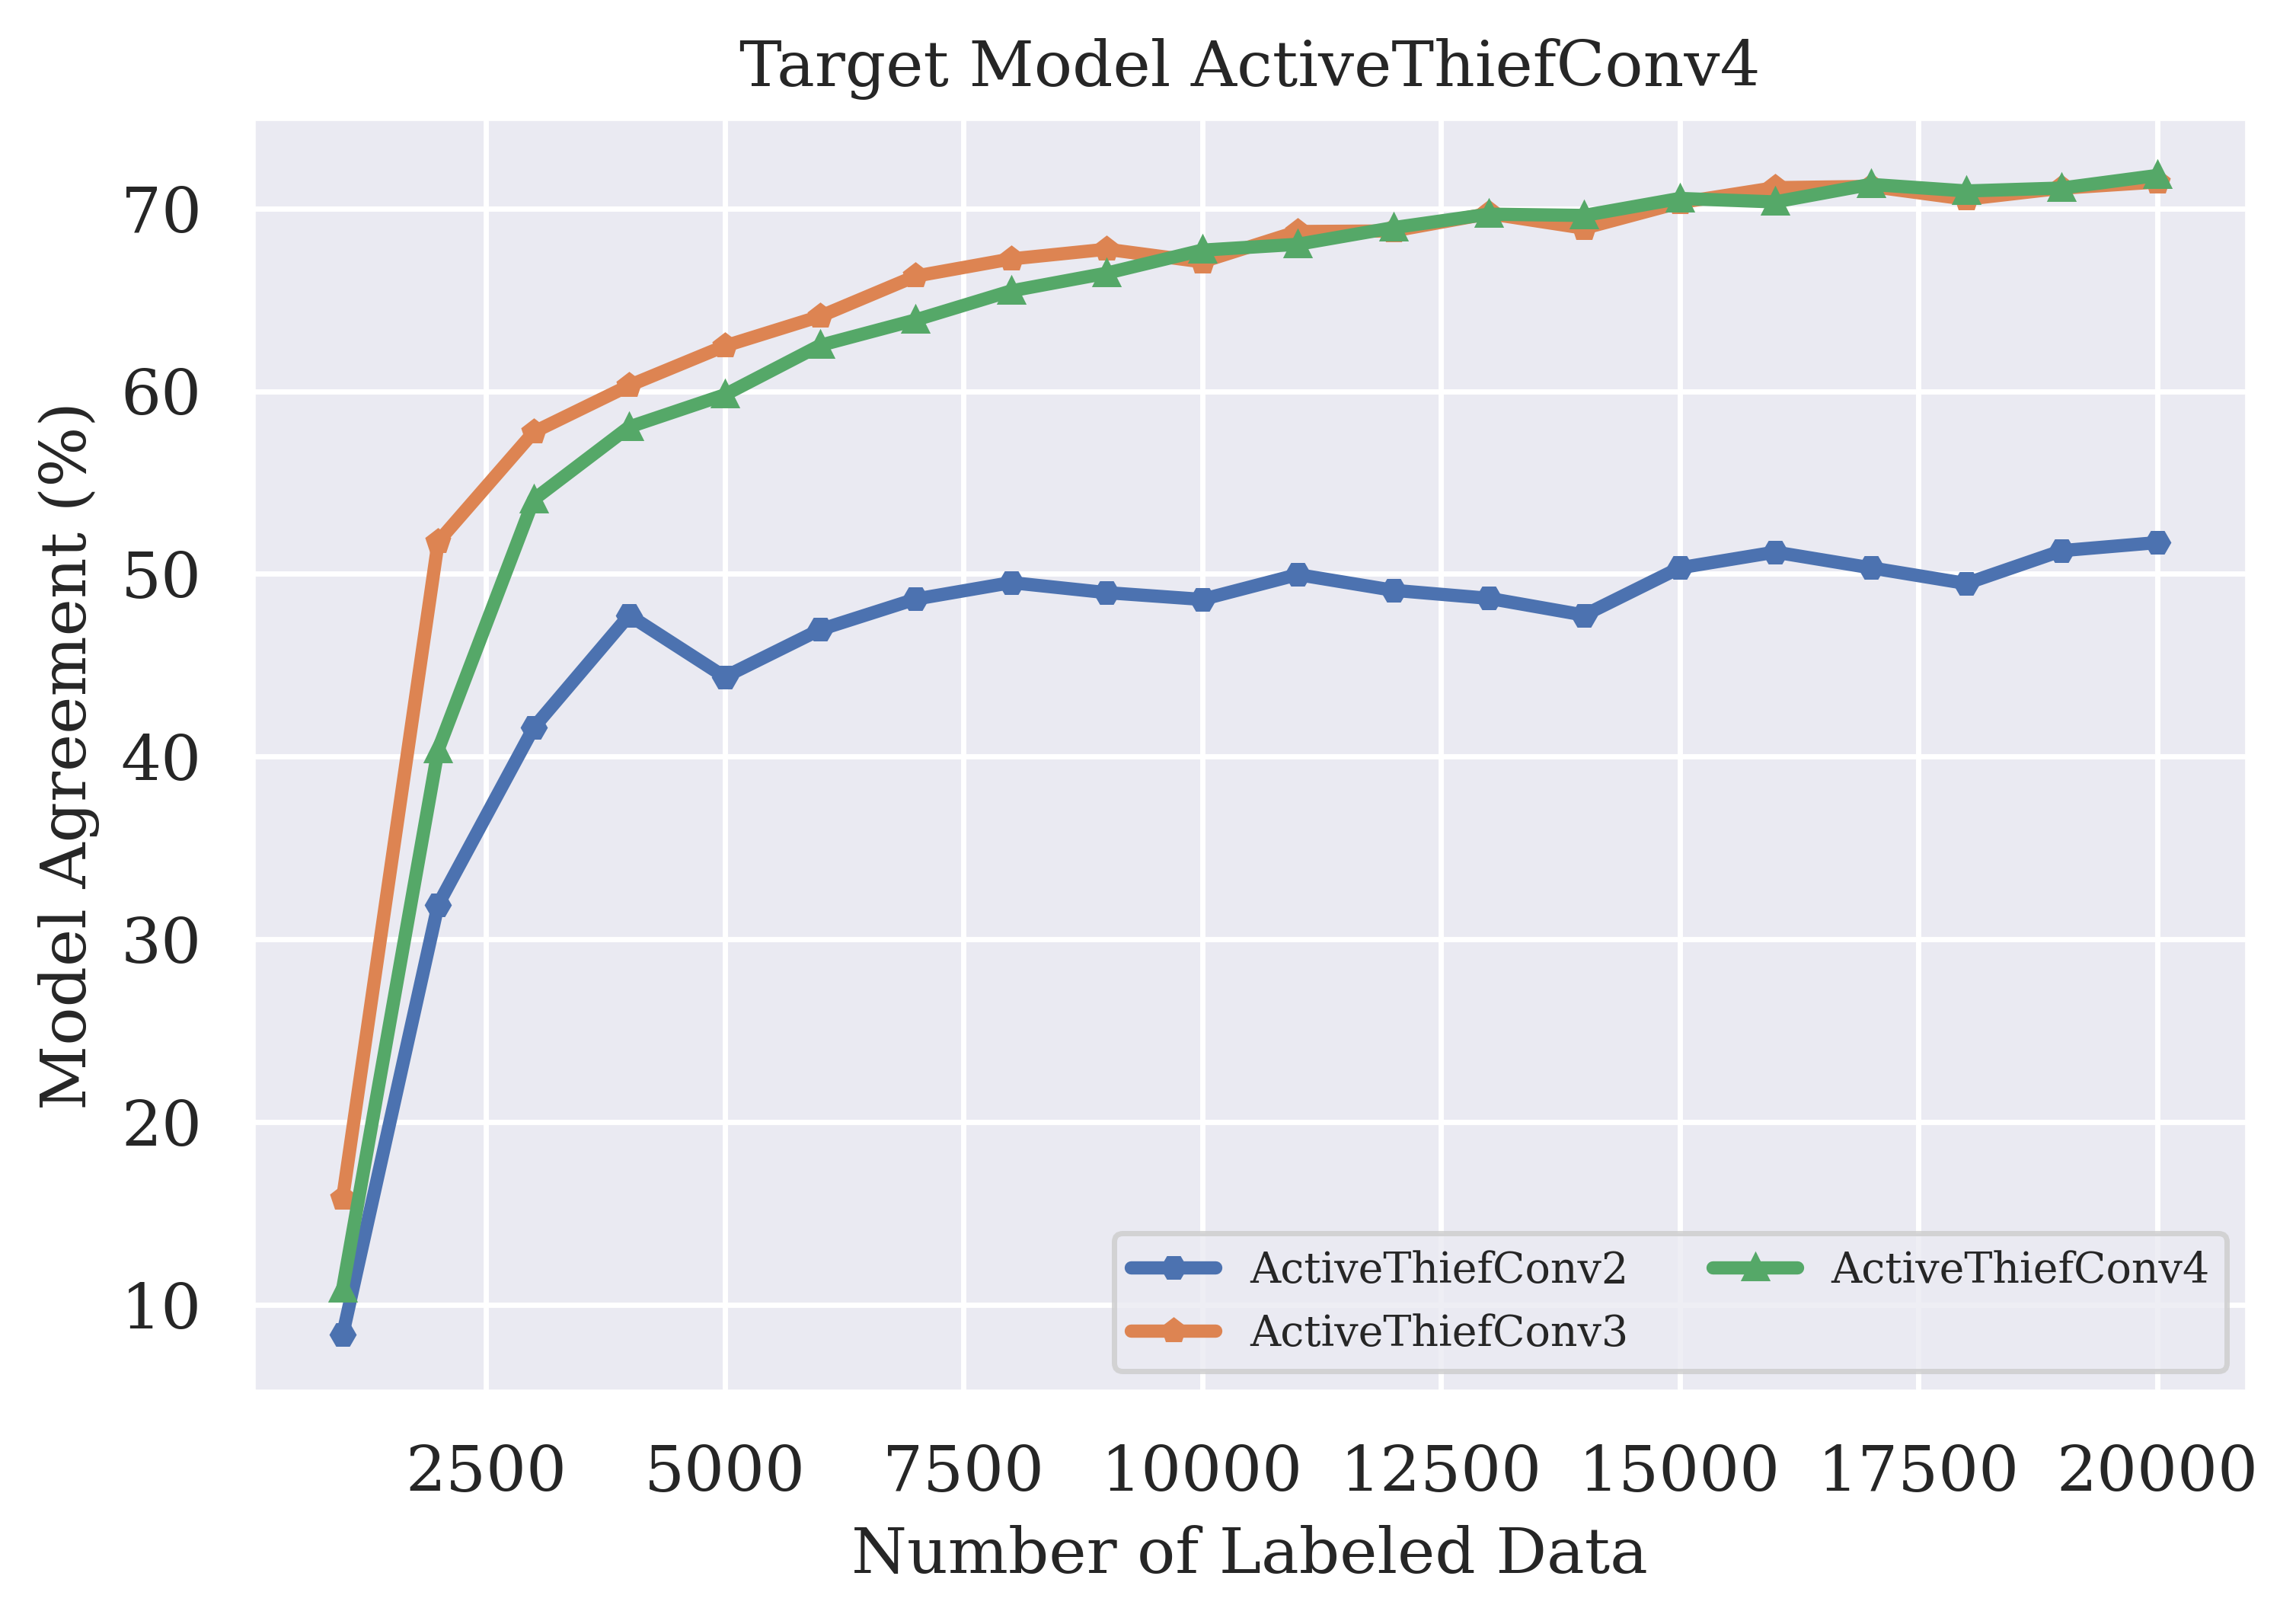
\includegraphics[width=0.32\linewidth]{images/MSInsights/cifar_act4.png}
    \caption{Agreement progression with varying model architectures on CIFAR-10.}
    \label{fig:CIFAR10modelComp}
\end{figure}


After evaluating the influence of the target and substitute model architecture on the success of the model stealing attack, we evaluate how the thief dataset effects
model stealing attacks. Our motivation for this experiment is that Pal et al. mention having tested CIFAR-10 as a thief dataset without success. We perform a model
stealing attack using ActiveThiefConv3 as the target and substitute model and CoreSet with batch size 2,000 as our active learning strategy. The total query budget is
20,000. We use MNIST as the target model dataset and change between Small ImageNet, Tiny ImageNet, and CIFAR-10 as our thief datasets. The results of this experiment
can be seen in figure \ref{fig:Appendix:MS:ActiveThief:EffectDataset}. While model agreement increases throughout the experiment when using Small ImageNet, the model
agreement for Tiny ImageNet plateaus after just three iterations at 20\%. Model stealing with CIFAR-10 yields the best results, however. At the end of the experiment,
the setup with CIFAR-10 as the thief dataset achieves a model agreement five percentage points higher than the setup with Small Imagenet. \par

\begin{figure}[!htb]
    \centering
    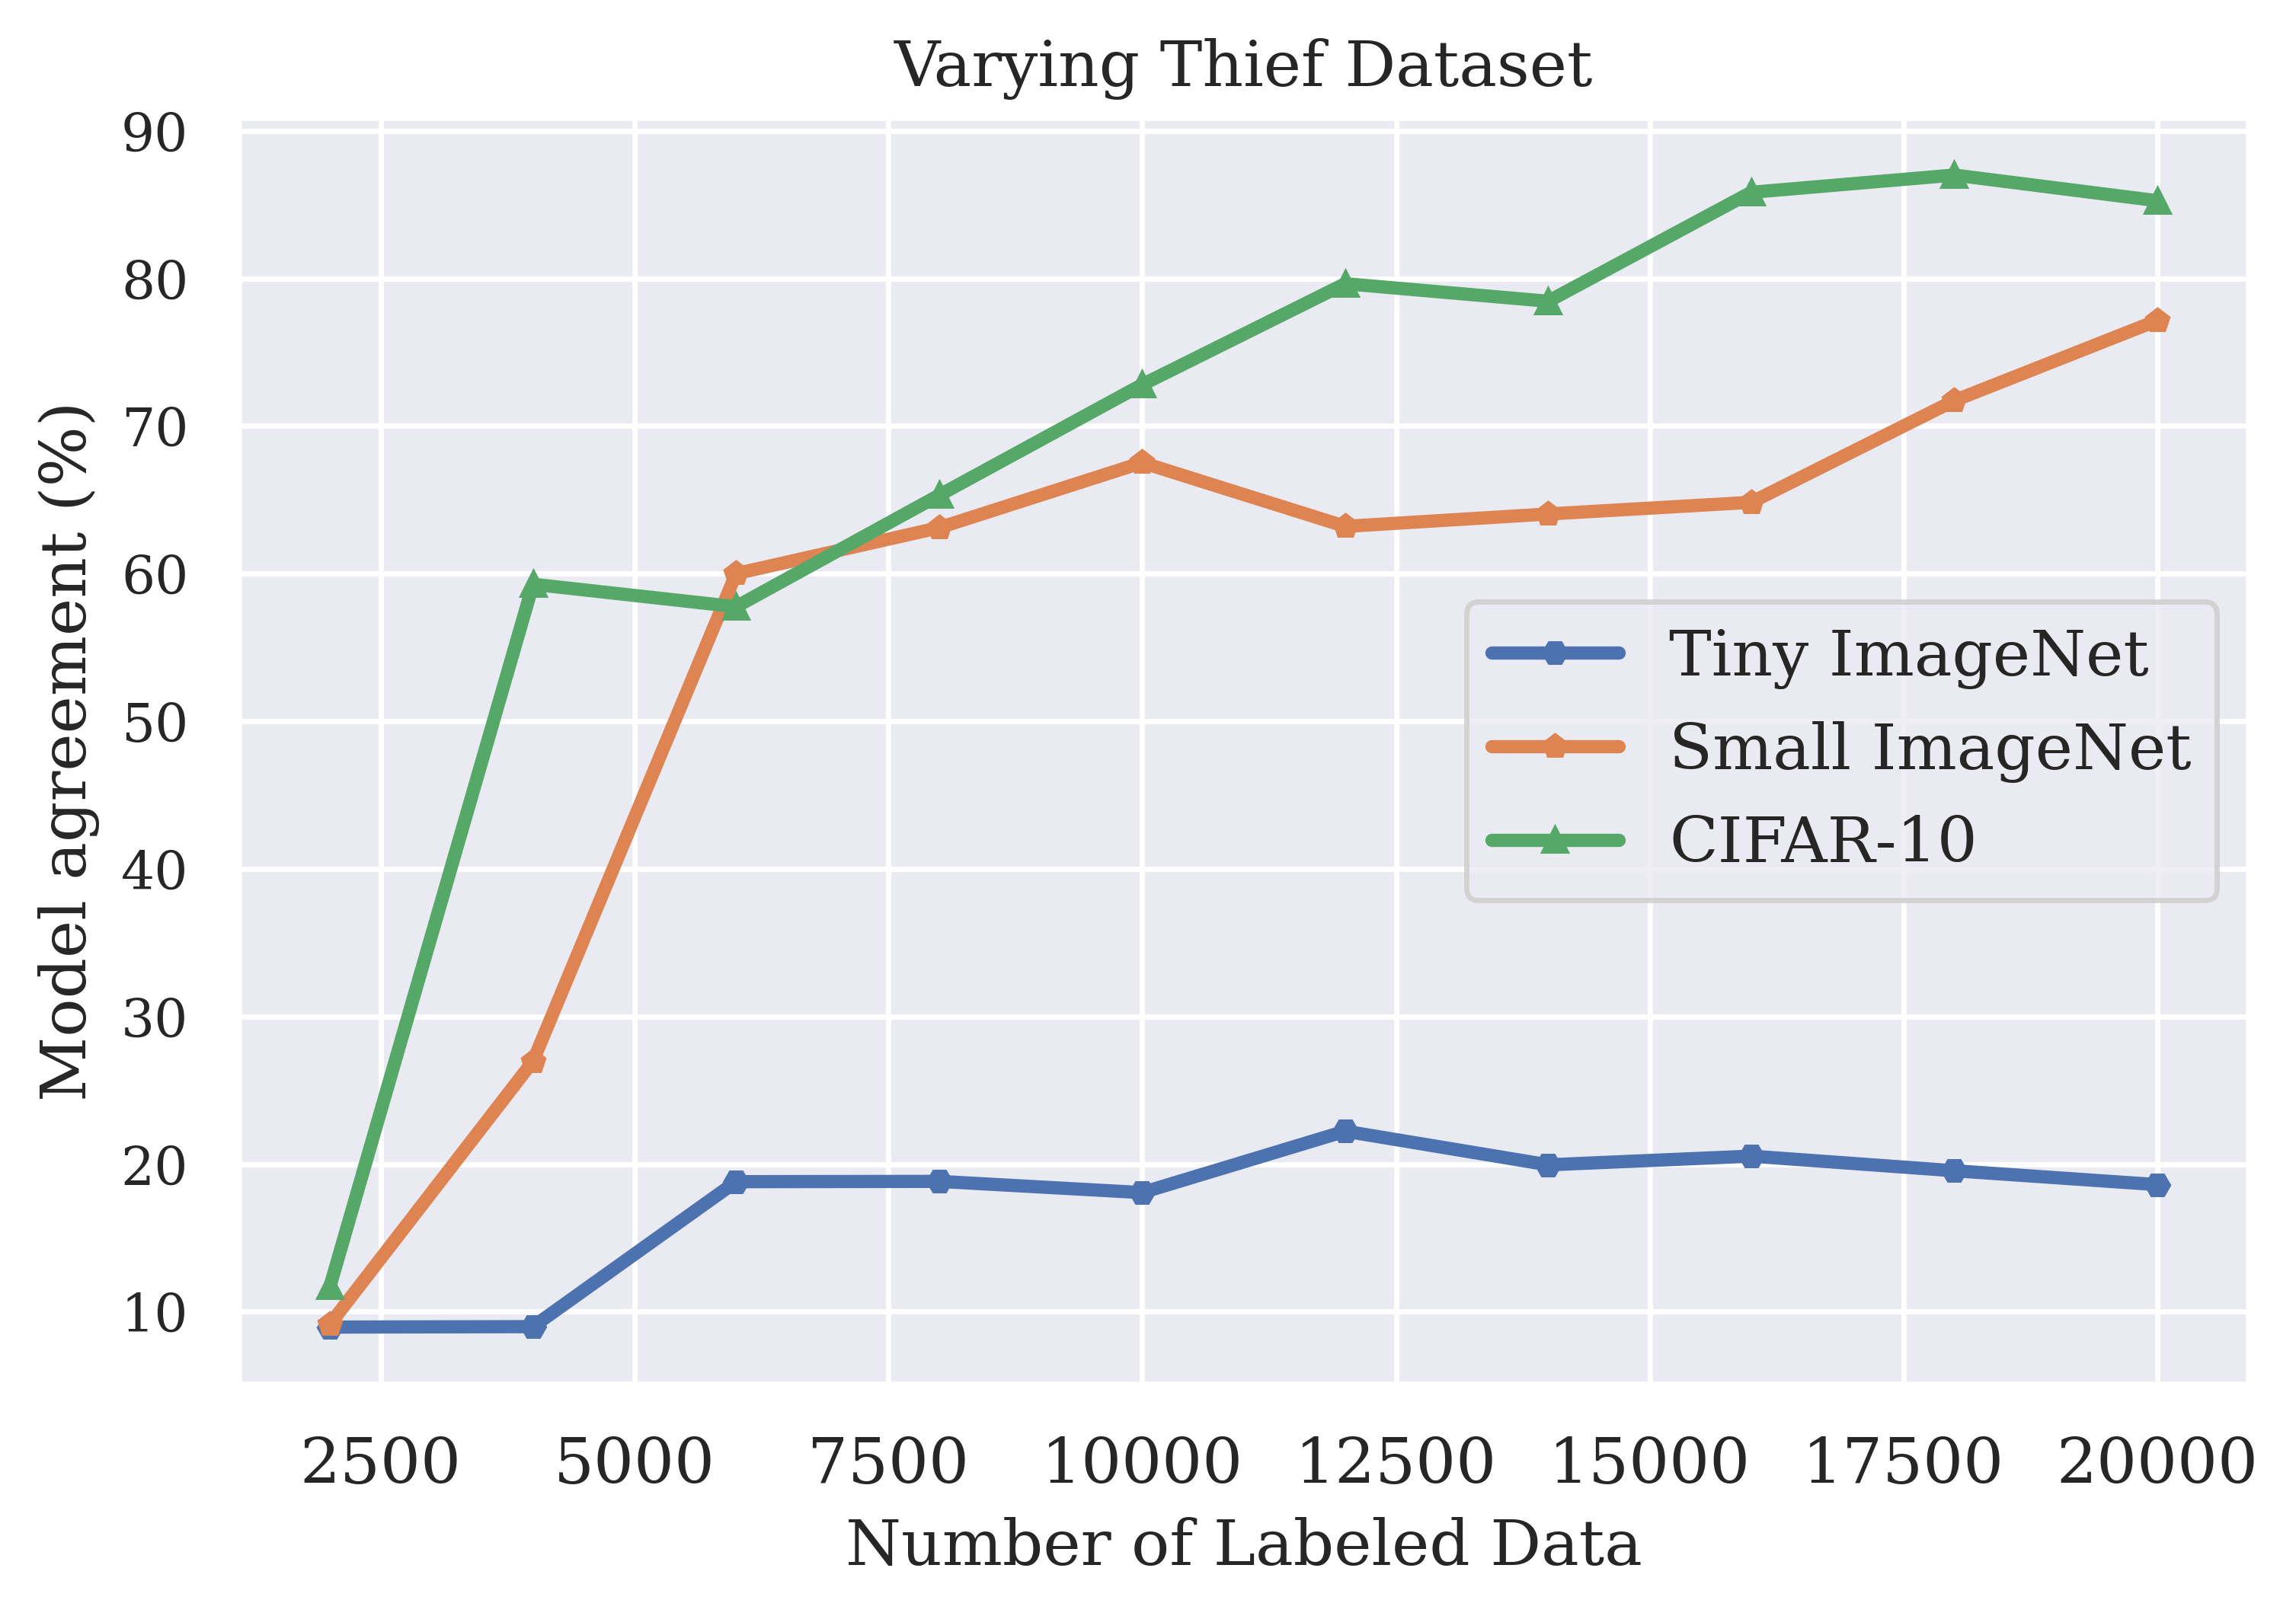
\includegraphics[width=0.8\linewidth]{images/results_CALMS/effect_dataset.png}
    \caption{Comparison of model agreement for various thief datasets.}
    \label{fig:Appendix:MS:ActiveThief:EffectDataset}
\end{figure}

\clearpage


\subsection{Continual Active Learning for Model Stealing}
\label{sec:Appendix:CALMS}
This section contains plots of the complete runs of all experiments in section \ref{sec:Evaluation:MS}.

\subsubsection{MNIST}
\label{sec:Appendix:CALMS:MNIST}
In this section, we present the complete runs of all experiments which involve continual active learning using MNIST as a target model dataset.

\begin{figure}[!htb]
    \centering
    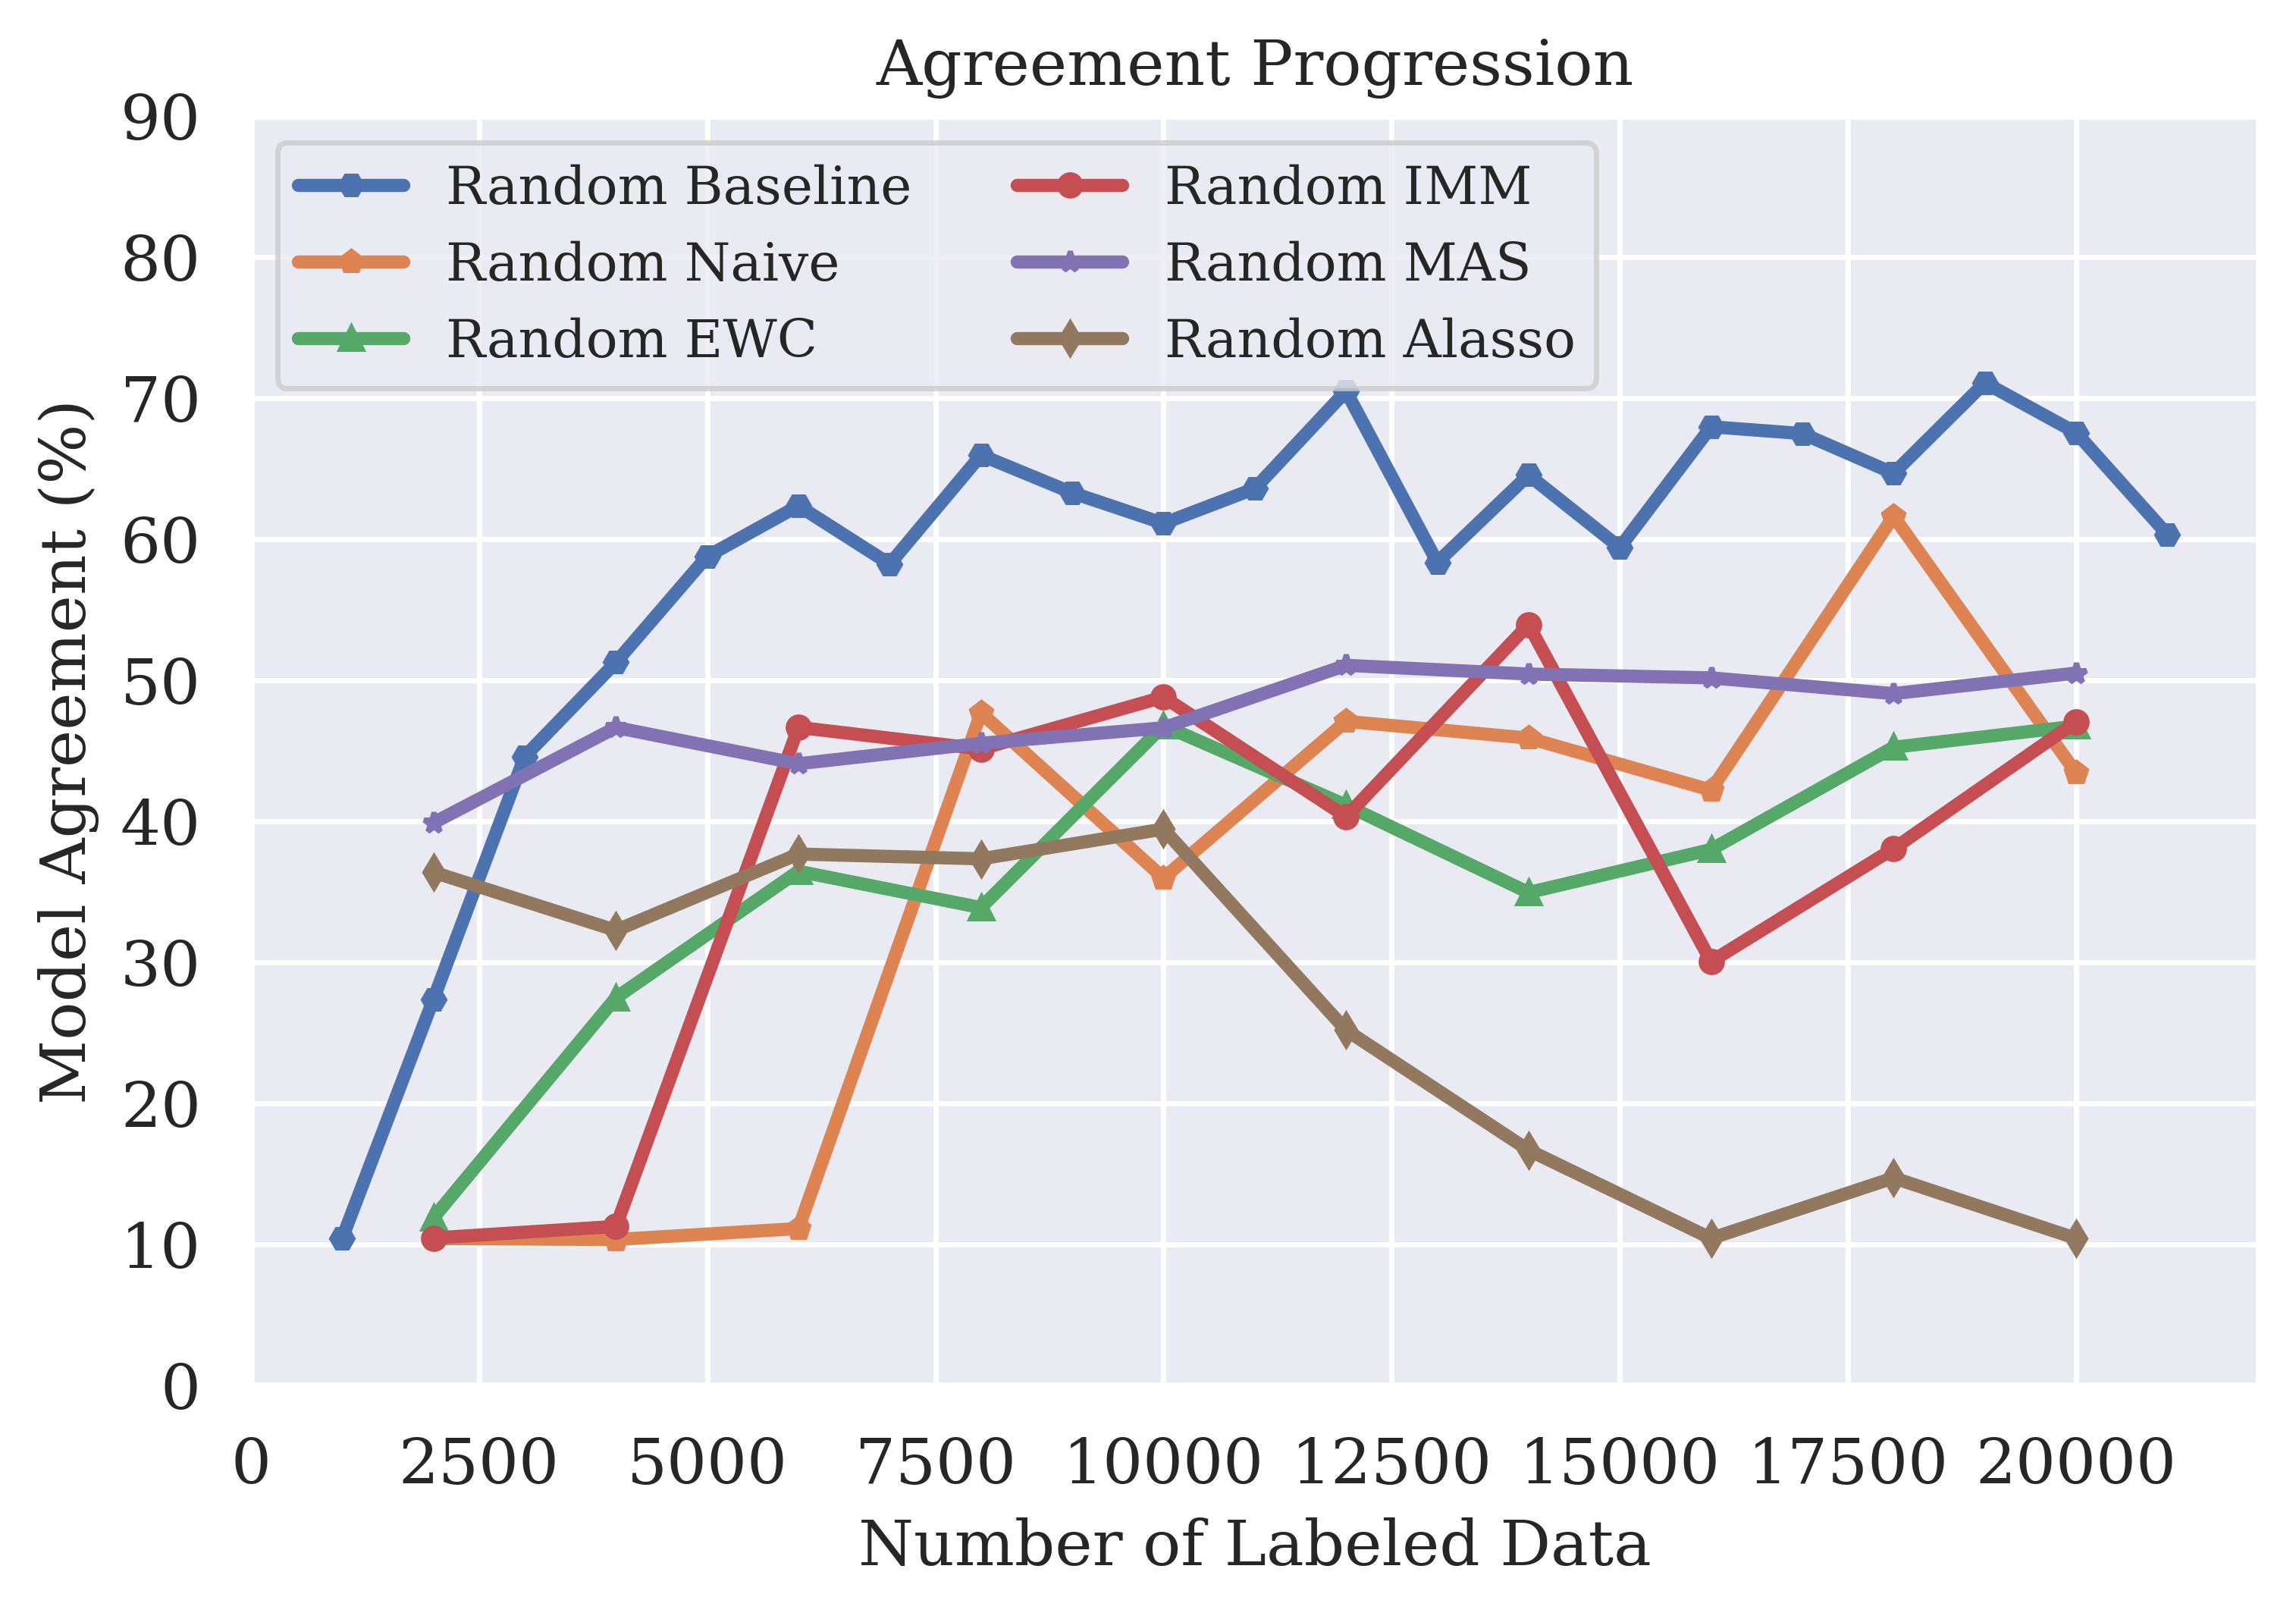
\includegraphics[width=0.48\linewidth]{images/results_CALMS/mnist_label_random.png} \hfill
    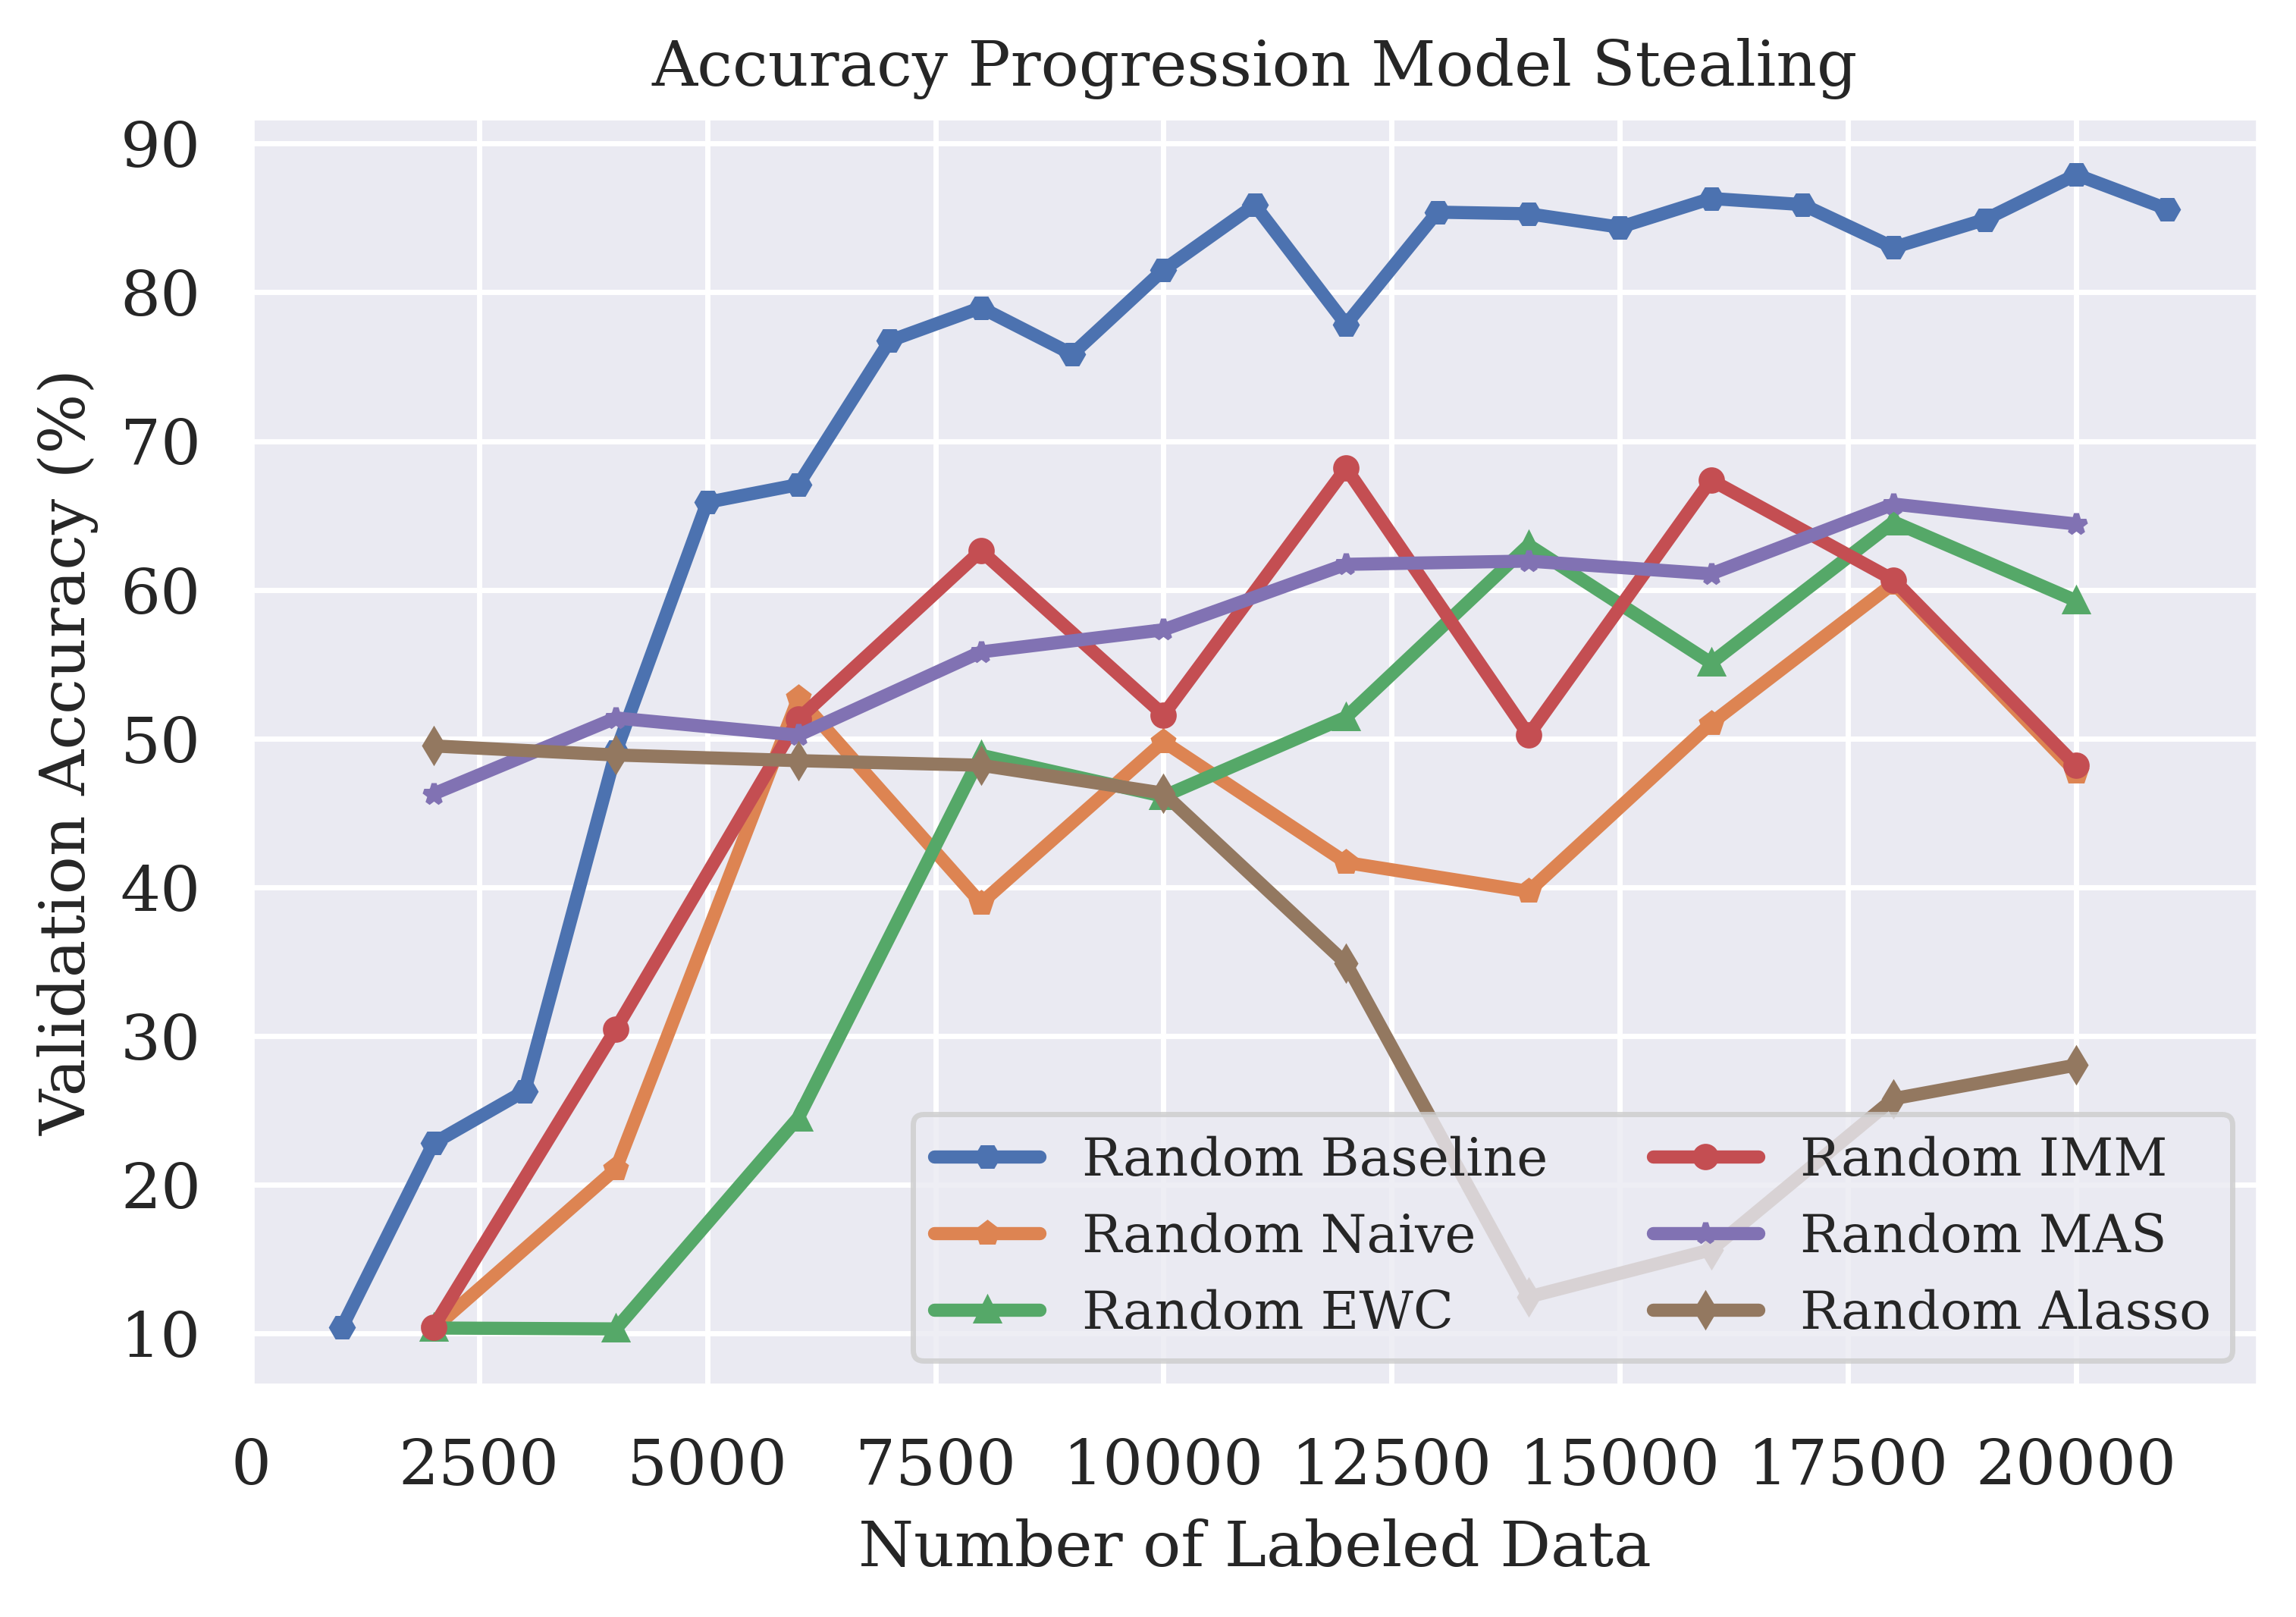
\includegraphics[width=0.48\linewidth]{images/results_CALMS/mnist_softmax_random.png}
    \caption{Agreement comparison for model stealing on MNIST using the active learning strategy Random.}
    \label{fig:CALMSMNISTRandom}
\end{figure}

\begin{figure}[!htb]
    \centering
    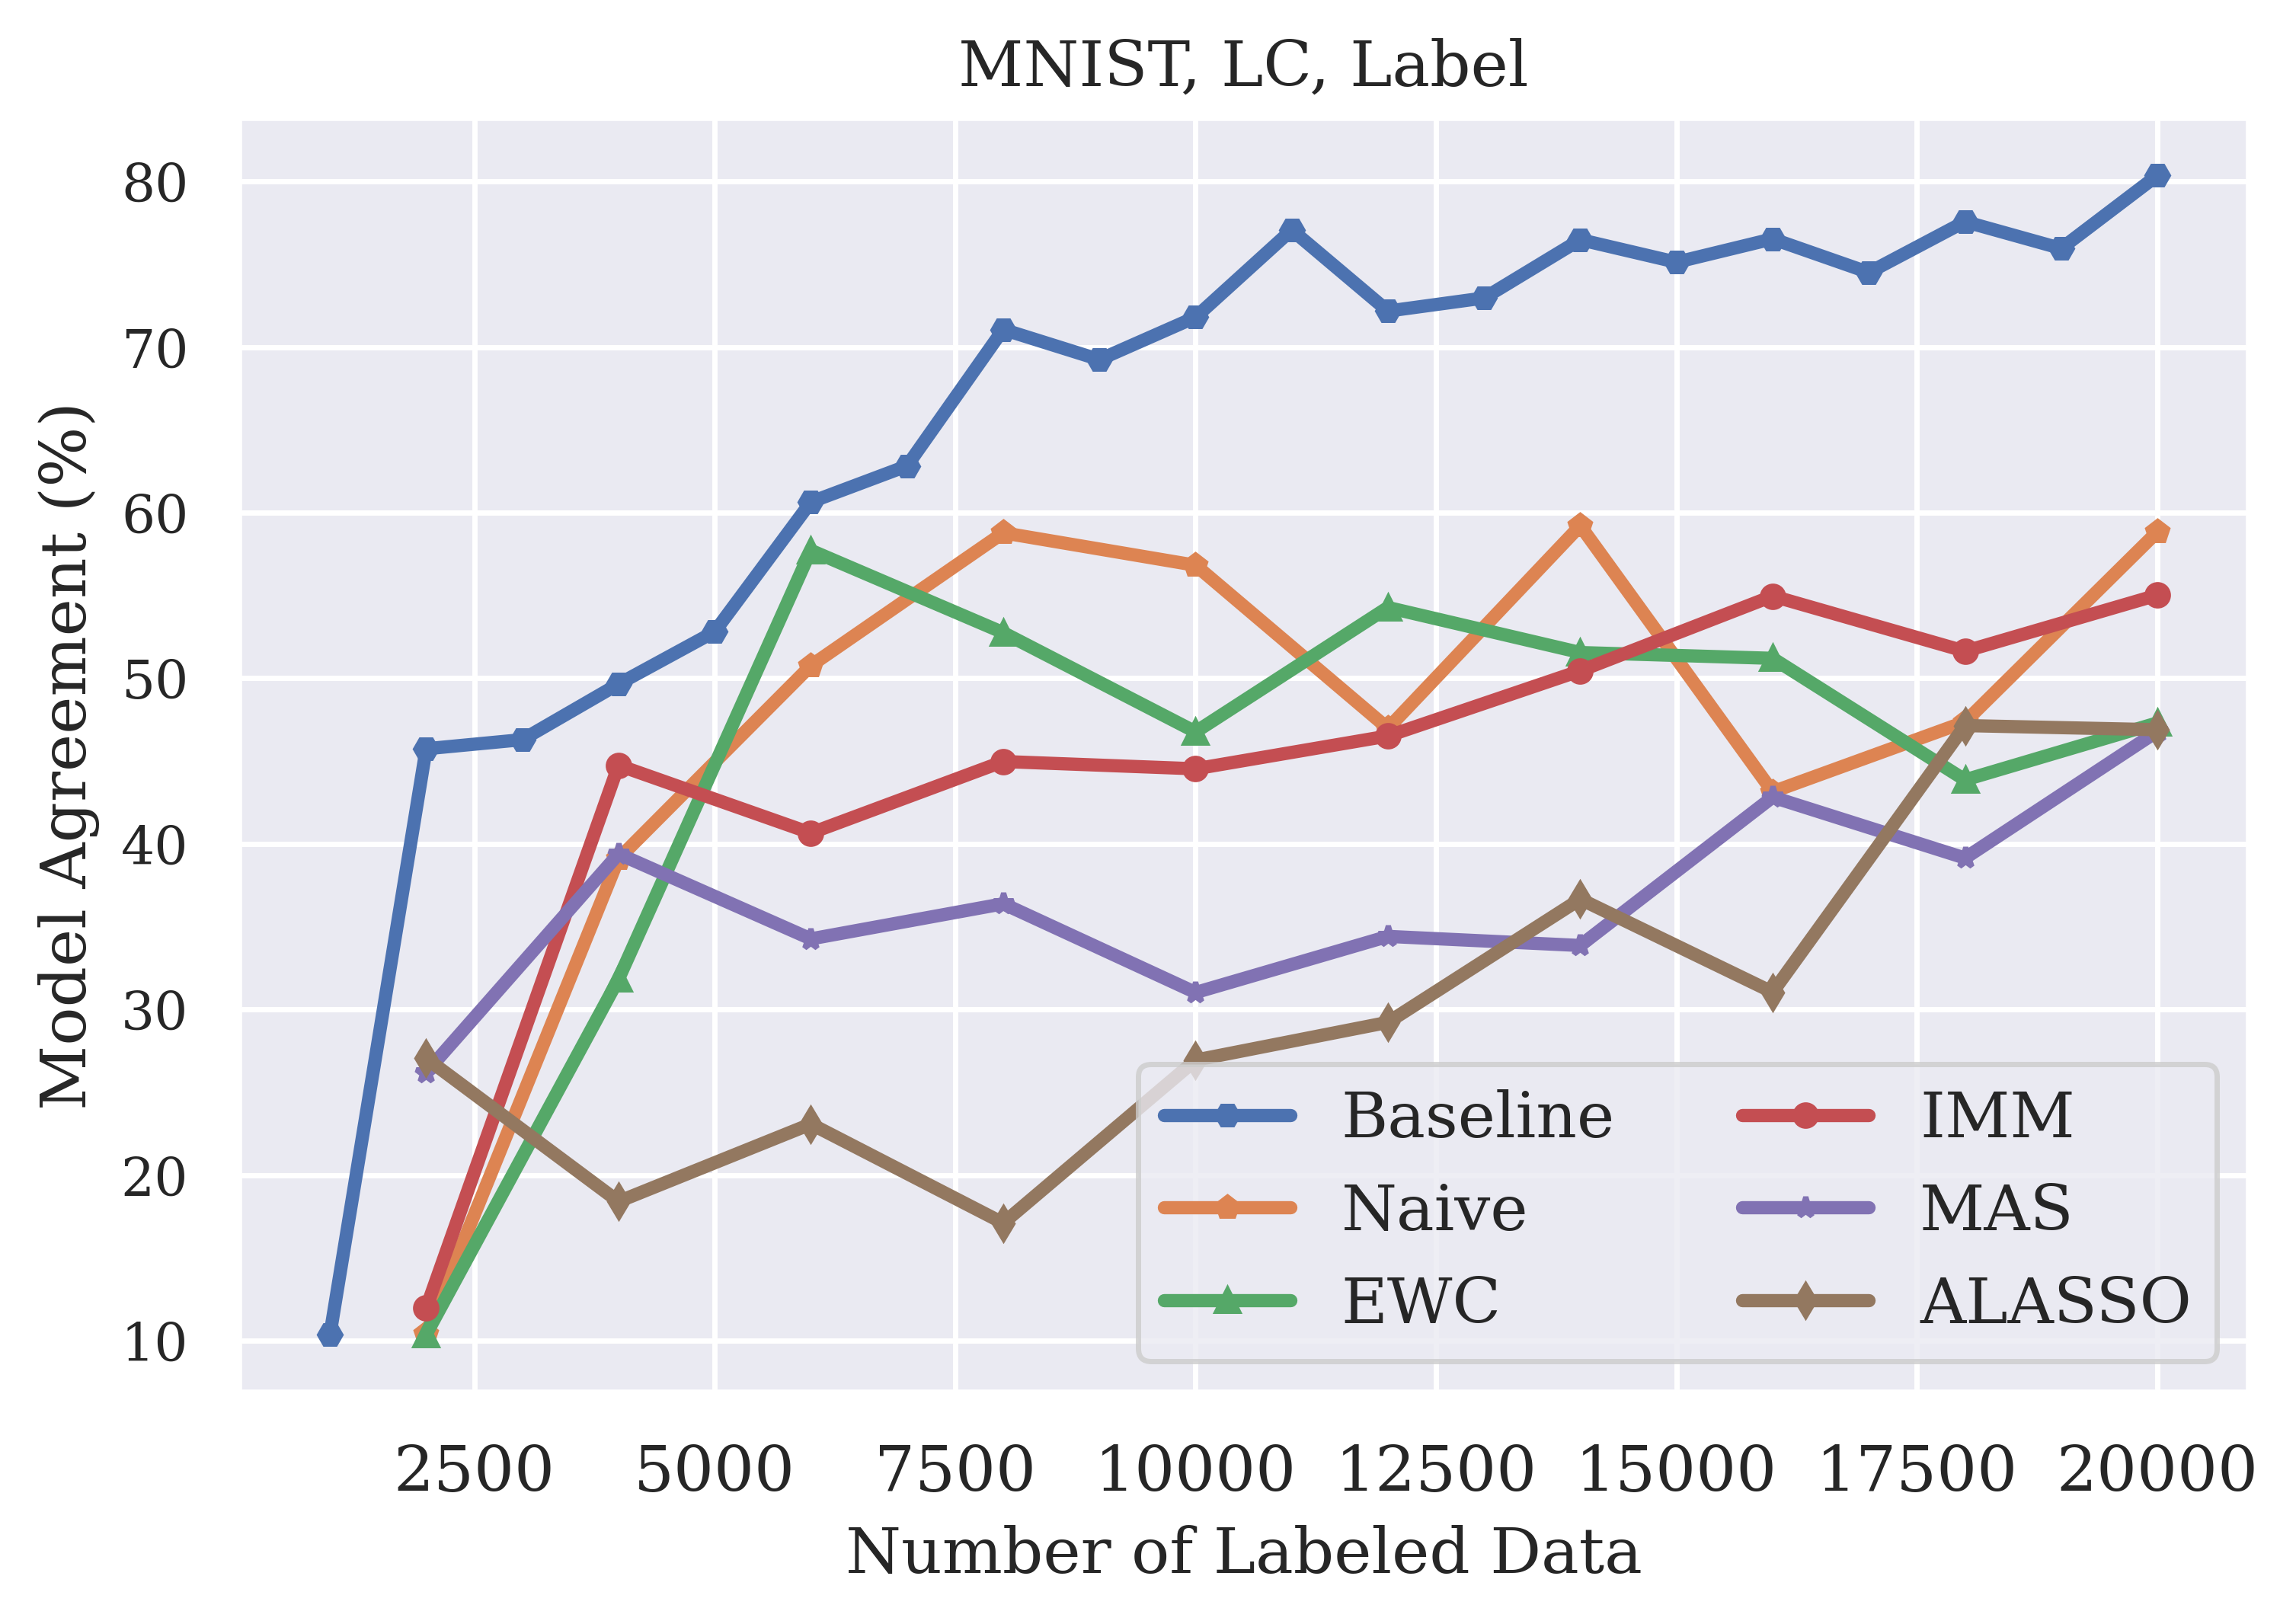
\includegraphics[width=0.48\linewidth]{images/results_CALMS/mnist_label_lc.png} \hfill
    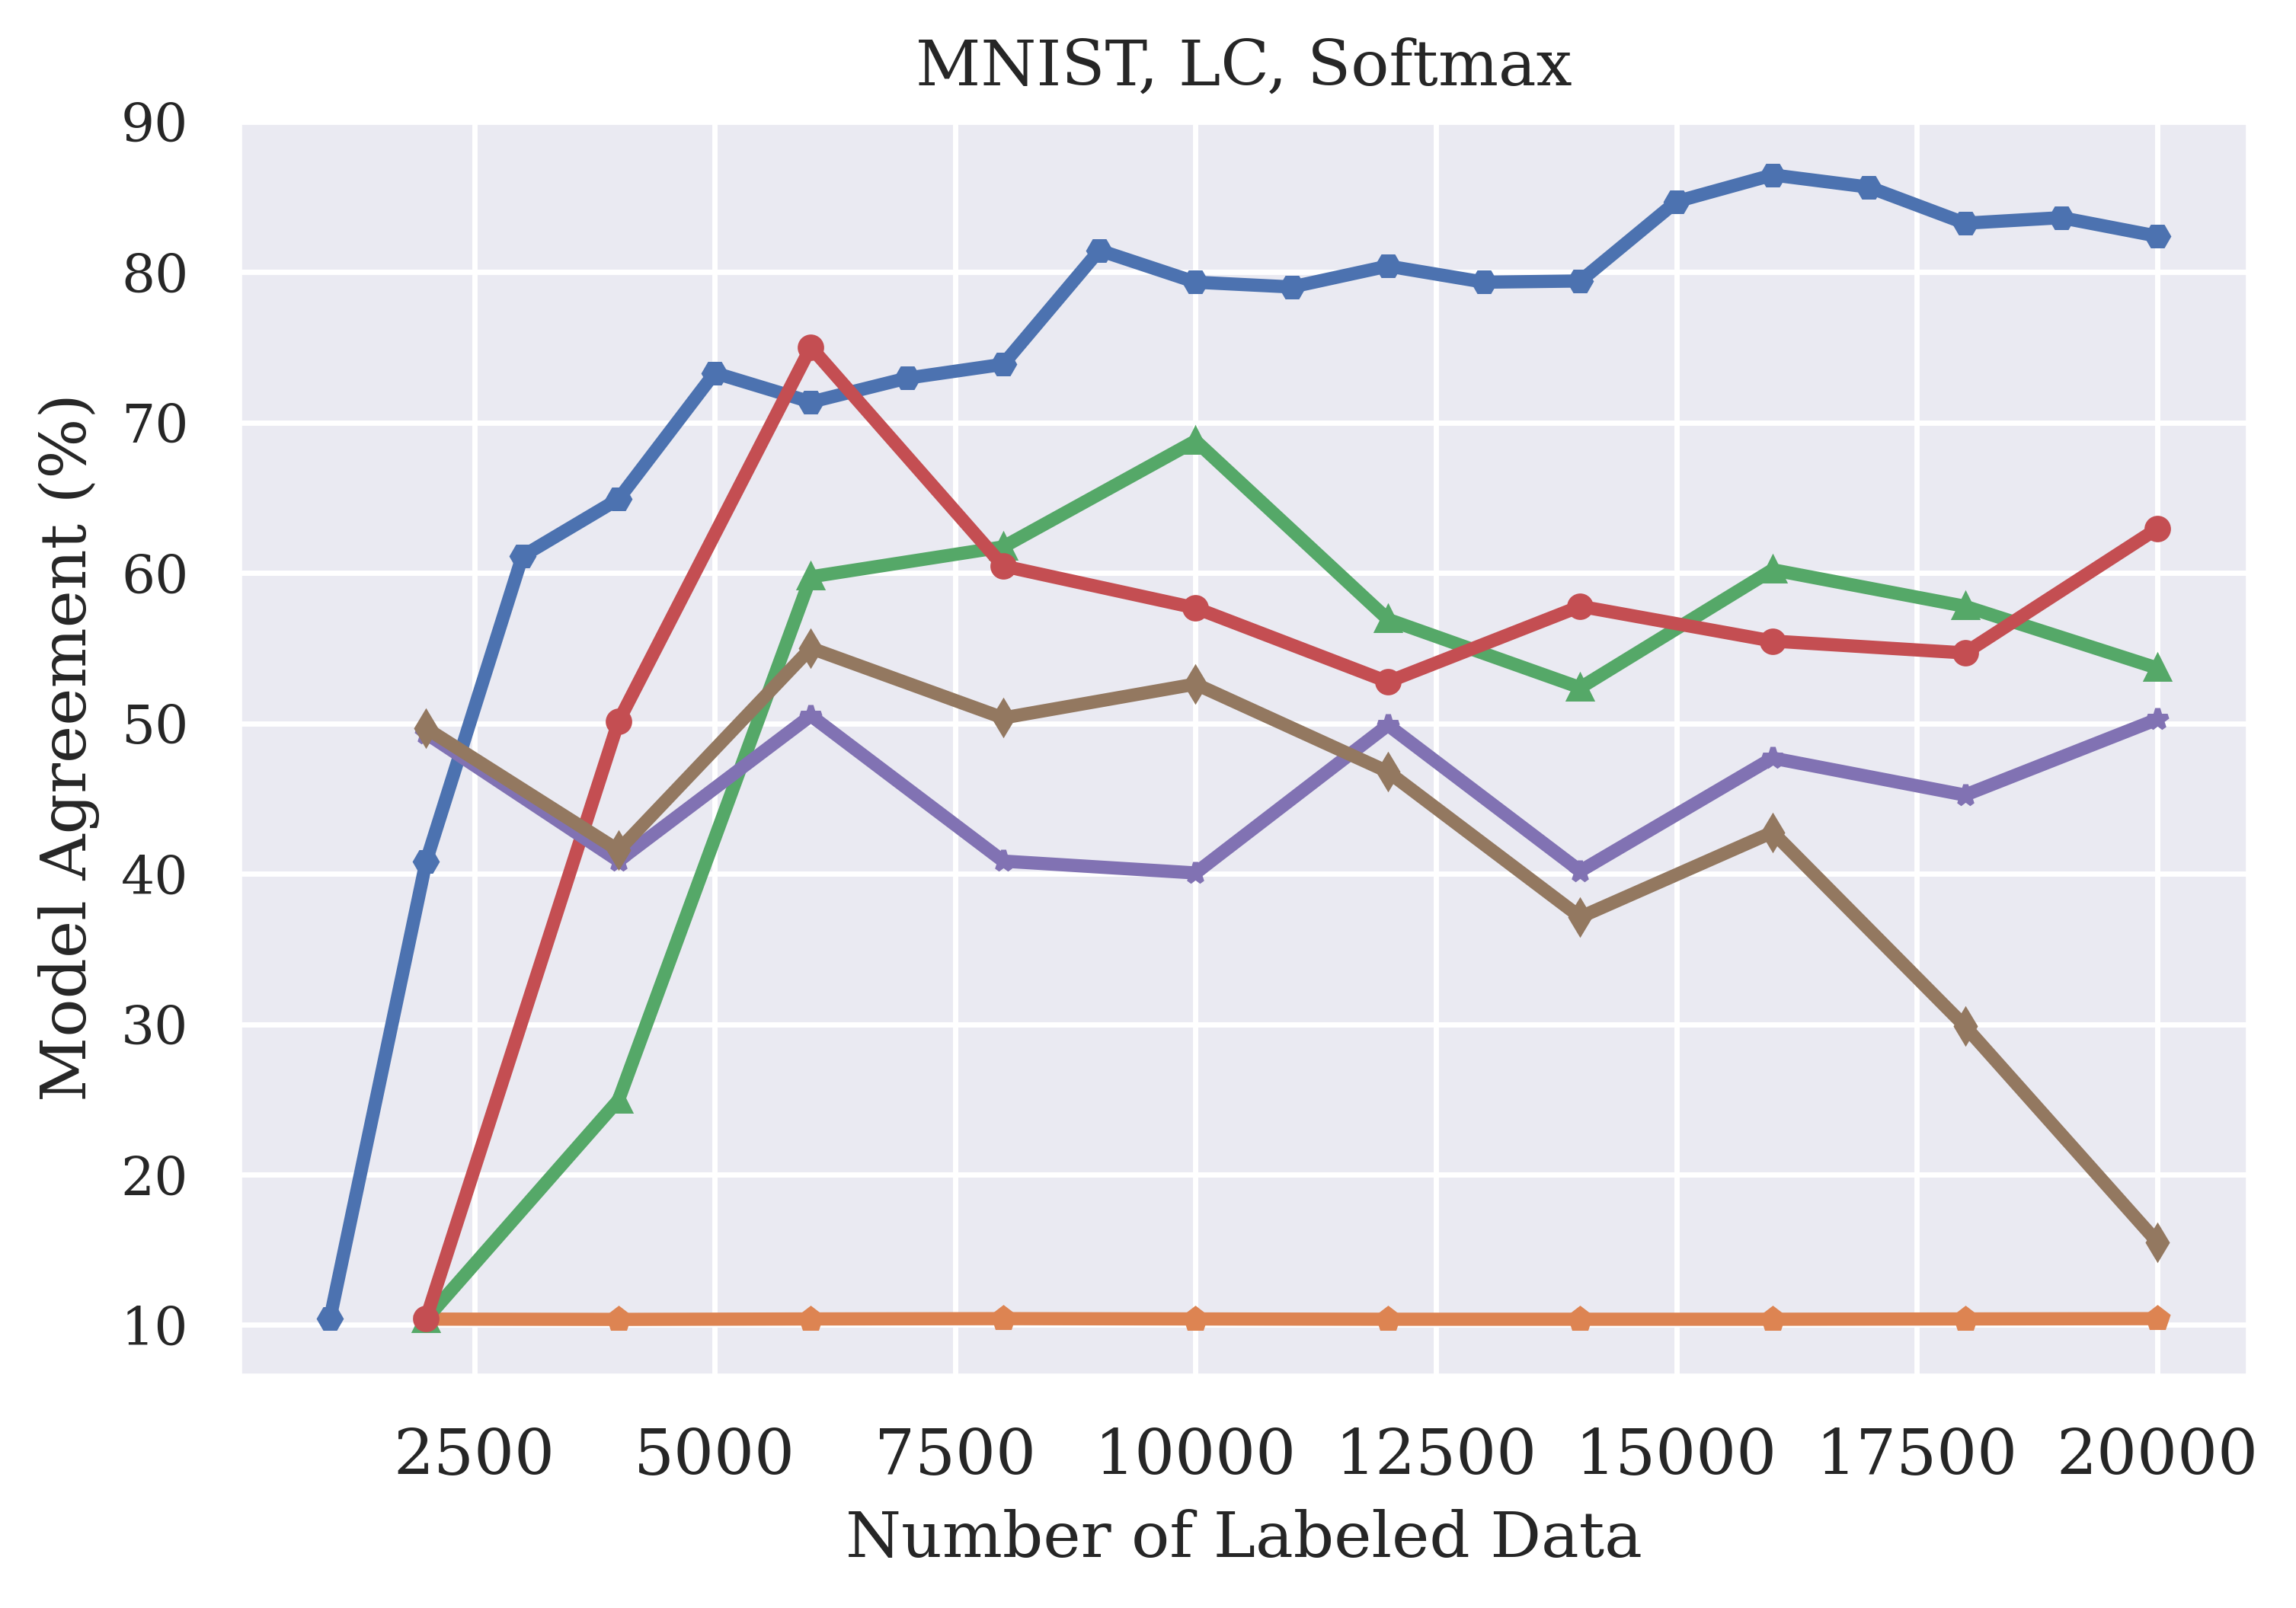
\includegraphics[width=0.48\linewidth]{images/results_CALMS/mnist_softmax_lc.png}
    \caption{Agreement comparison for model stealing on MNIST using the active learning strategy \gls{lc}.}
    \label{fig:CALMSMNISTLC}
\end{figure}

\begin{figure}[!htb]
    \centering
    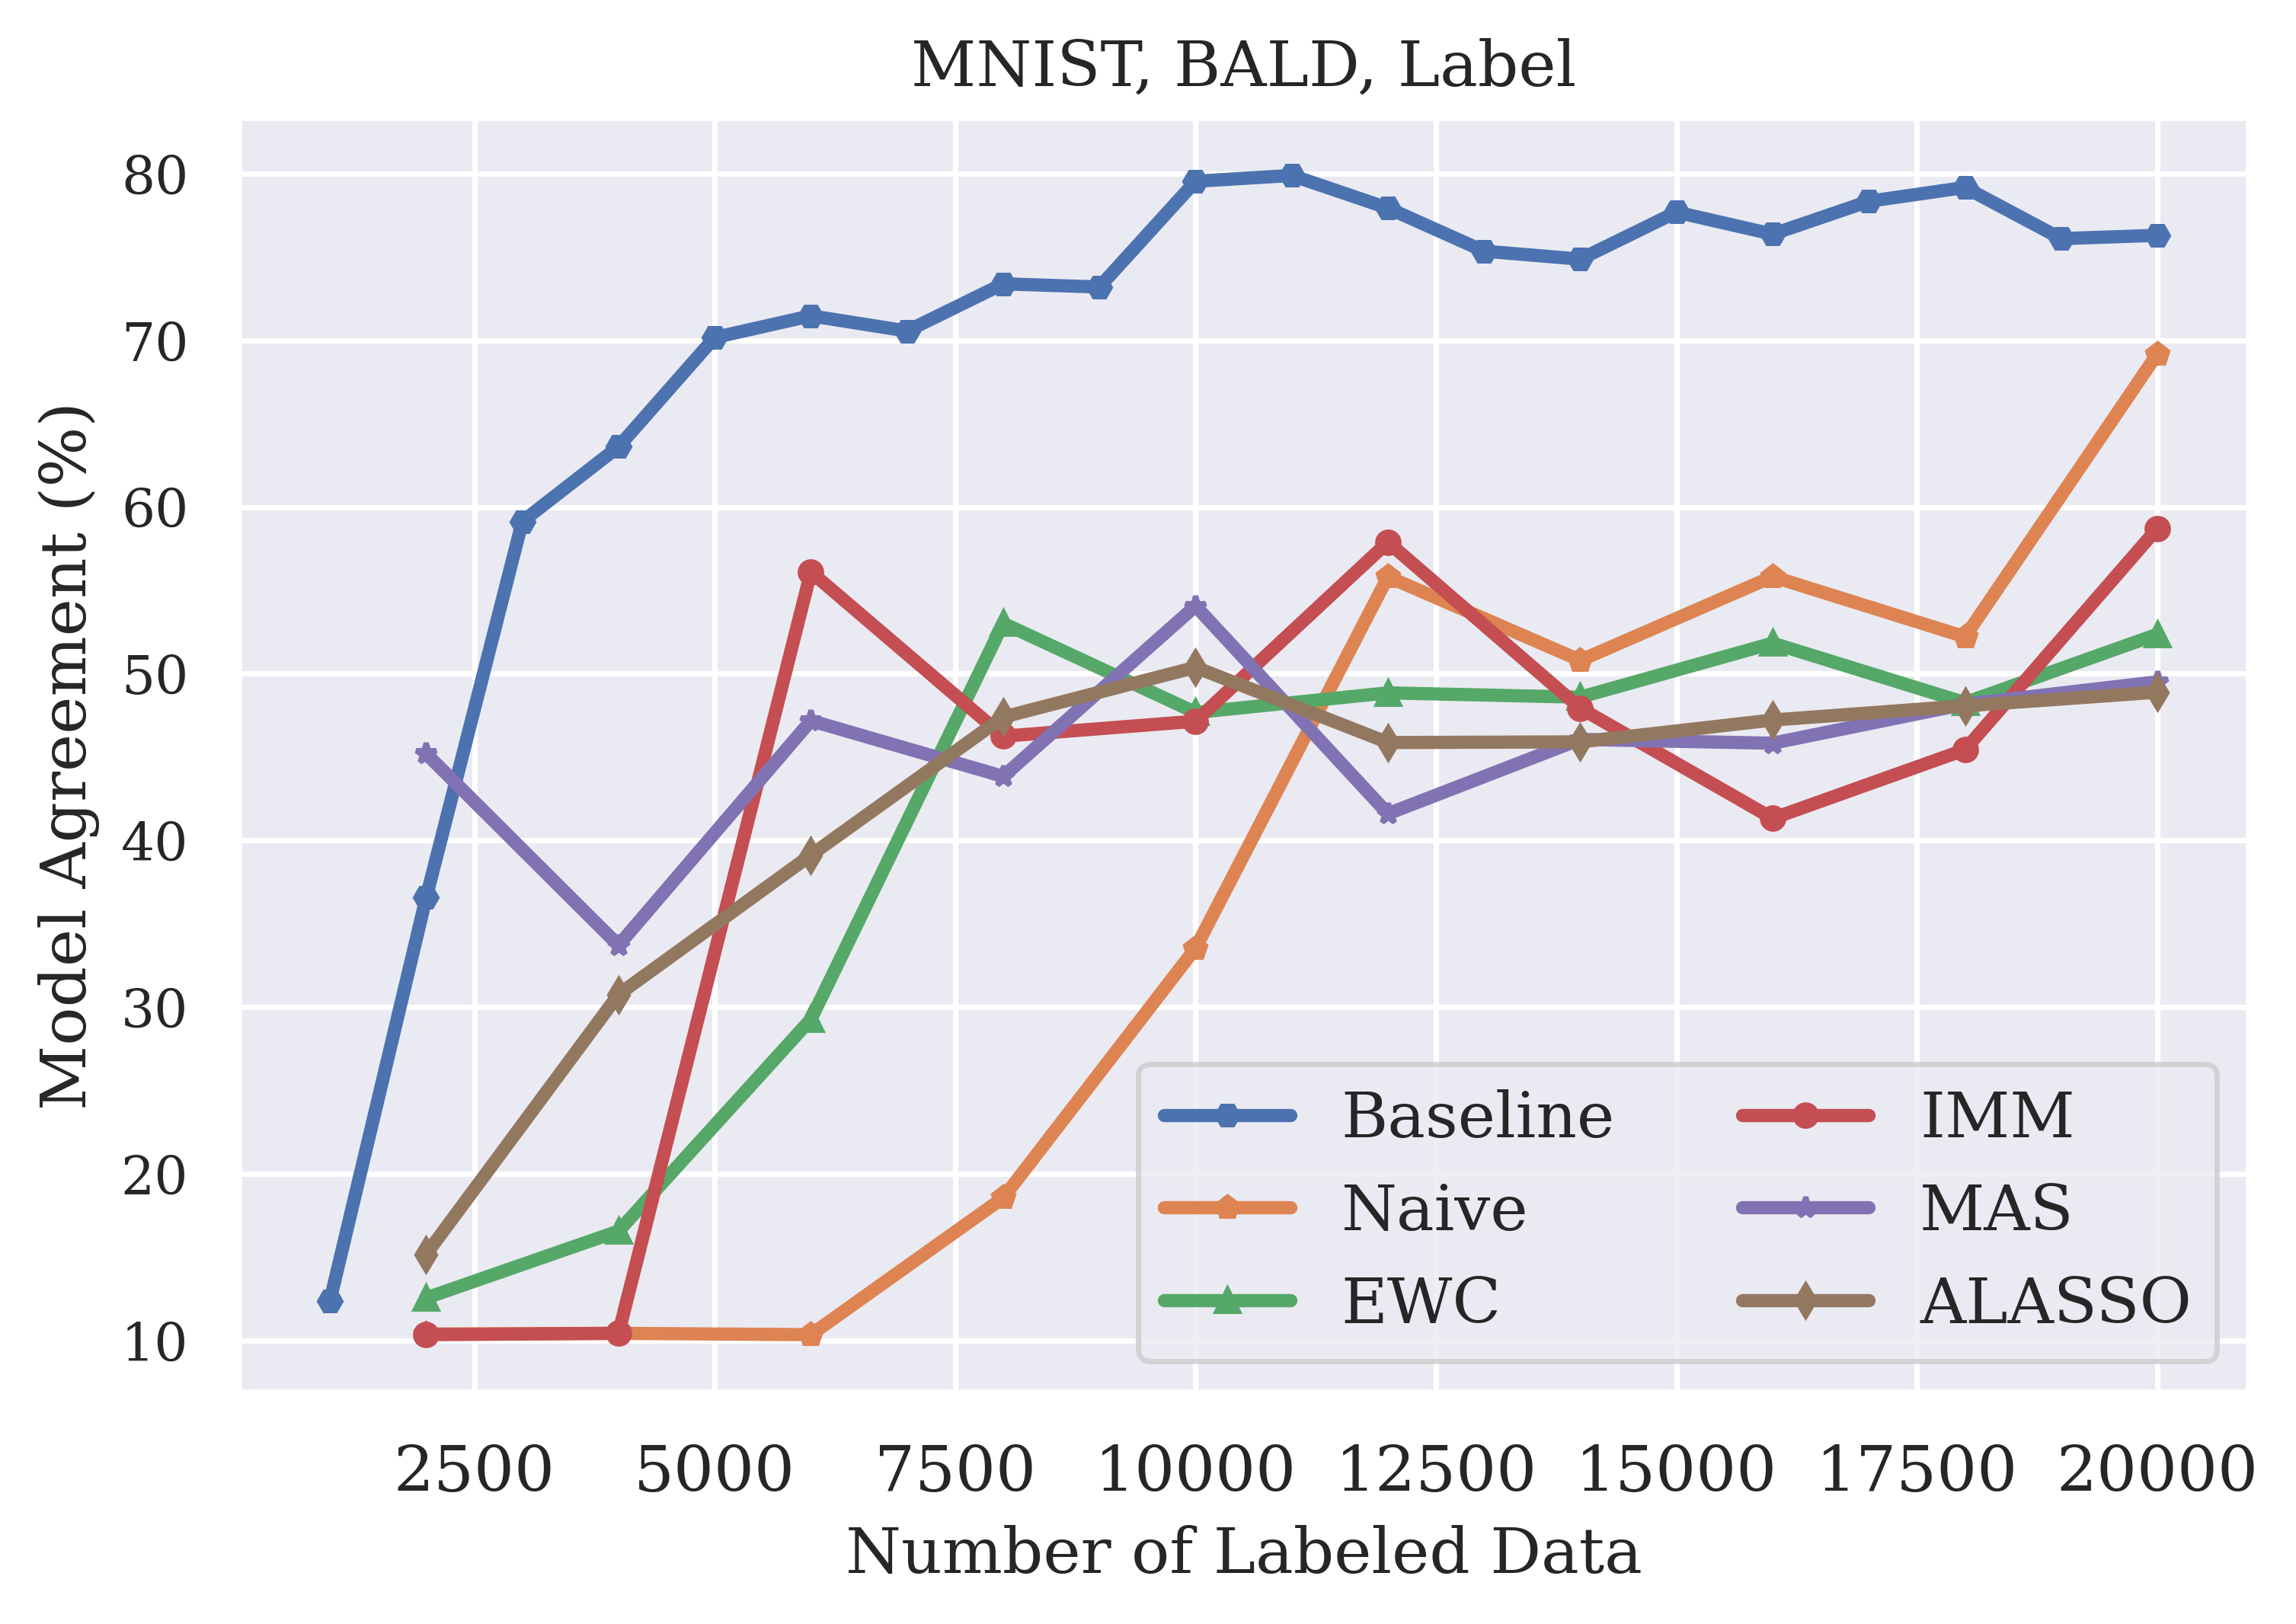
\includegraphics[width=0.48\linewidth]{images/results_CALMS/mnist_label_bald.png} \hfill
    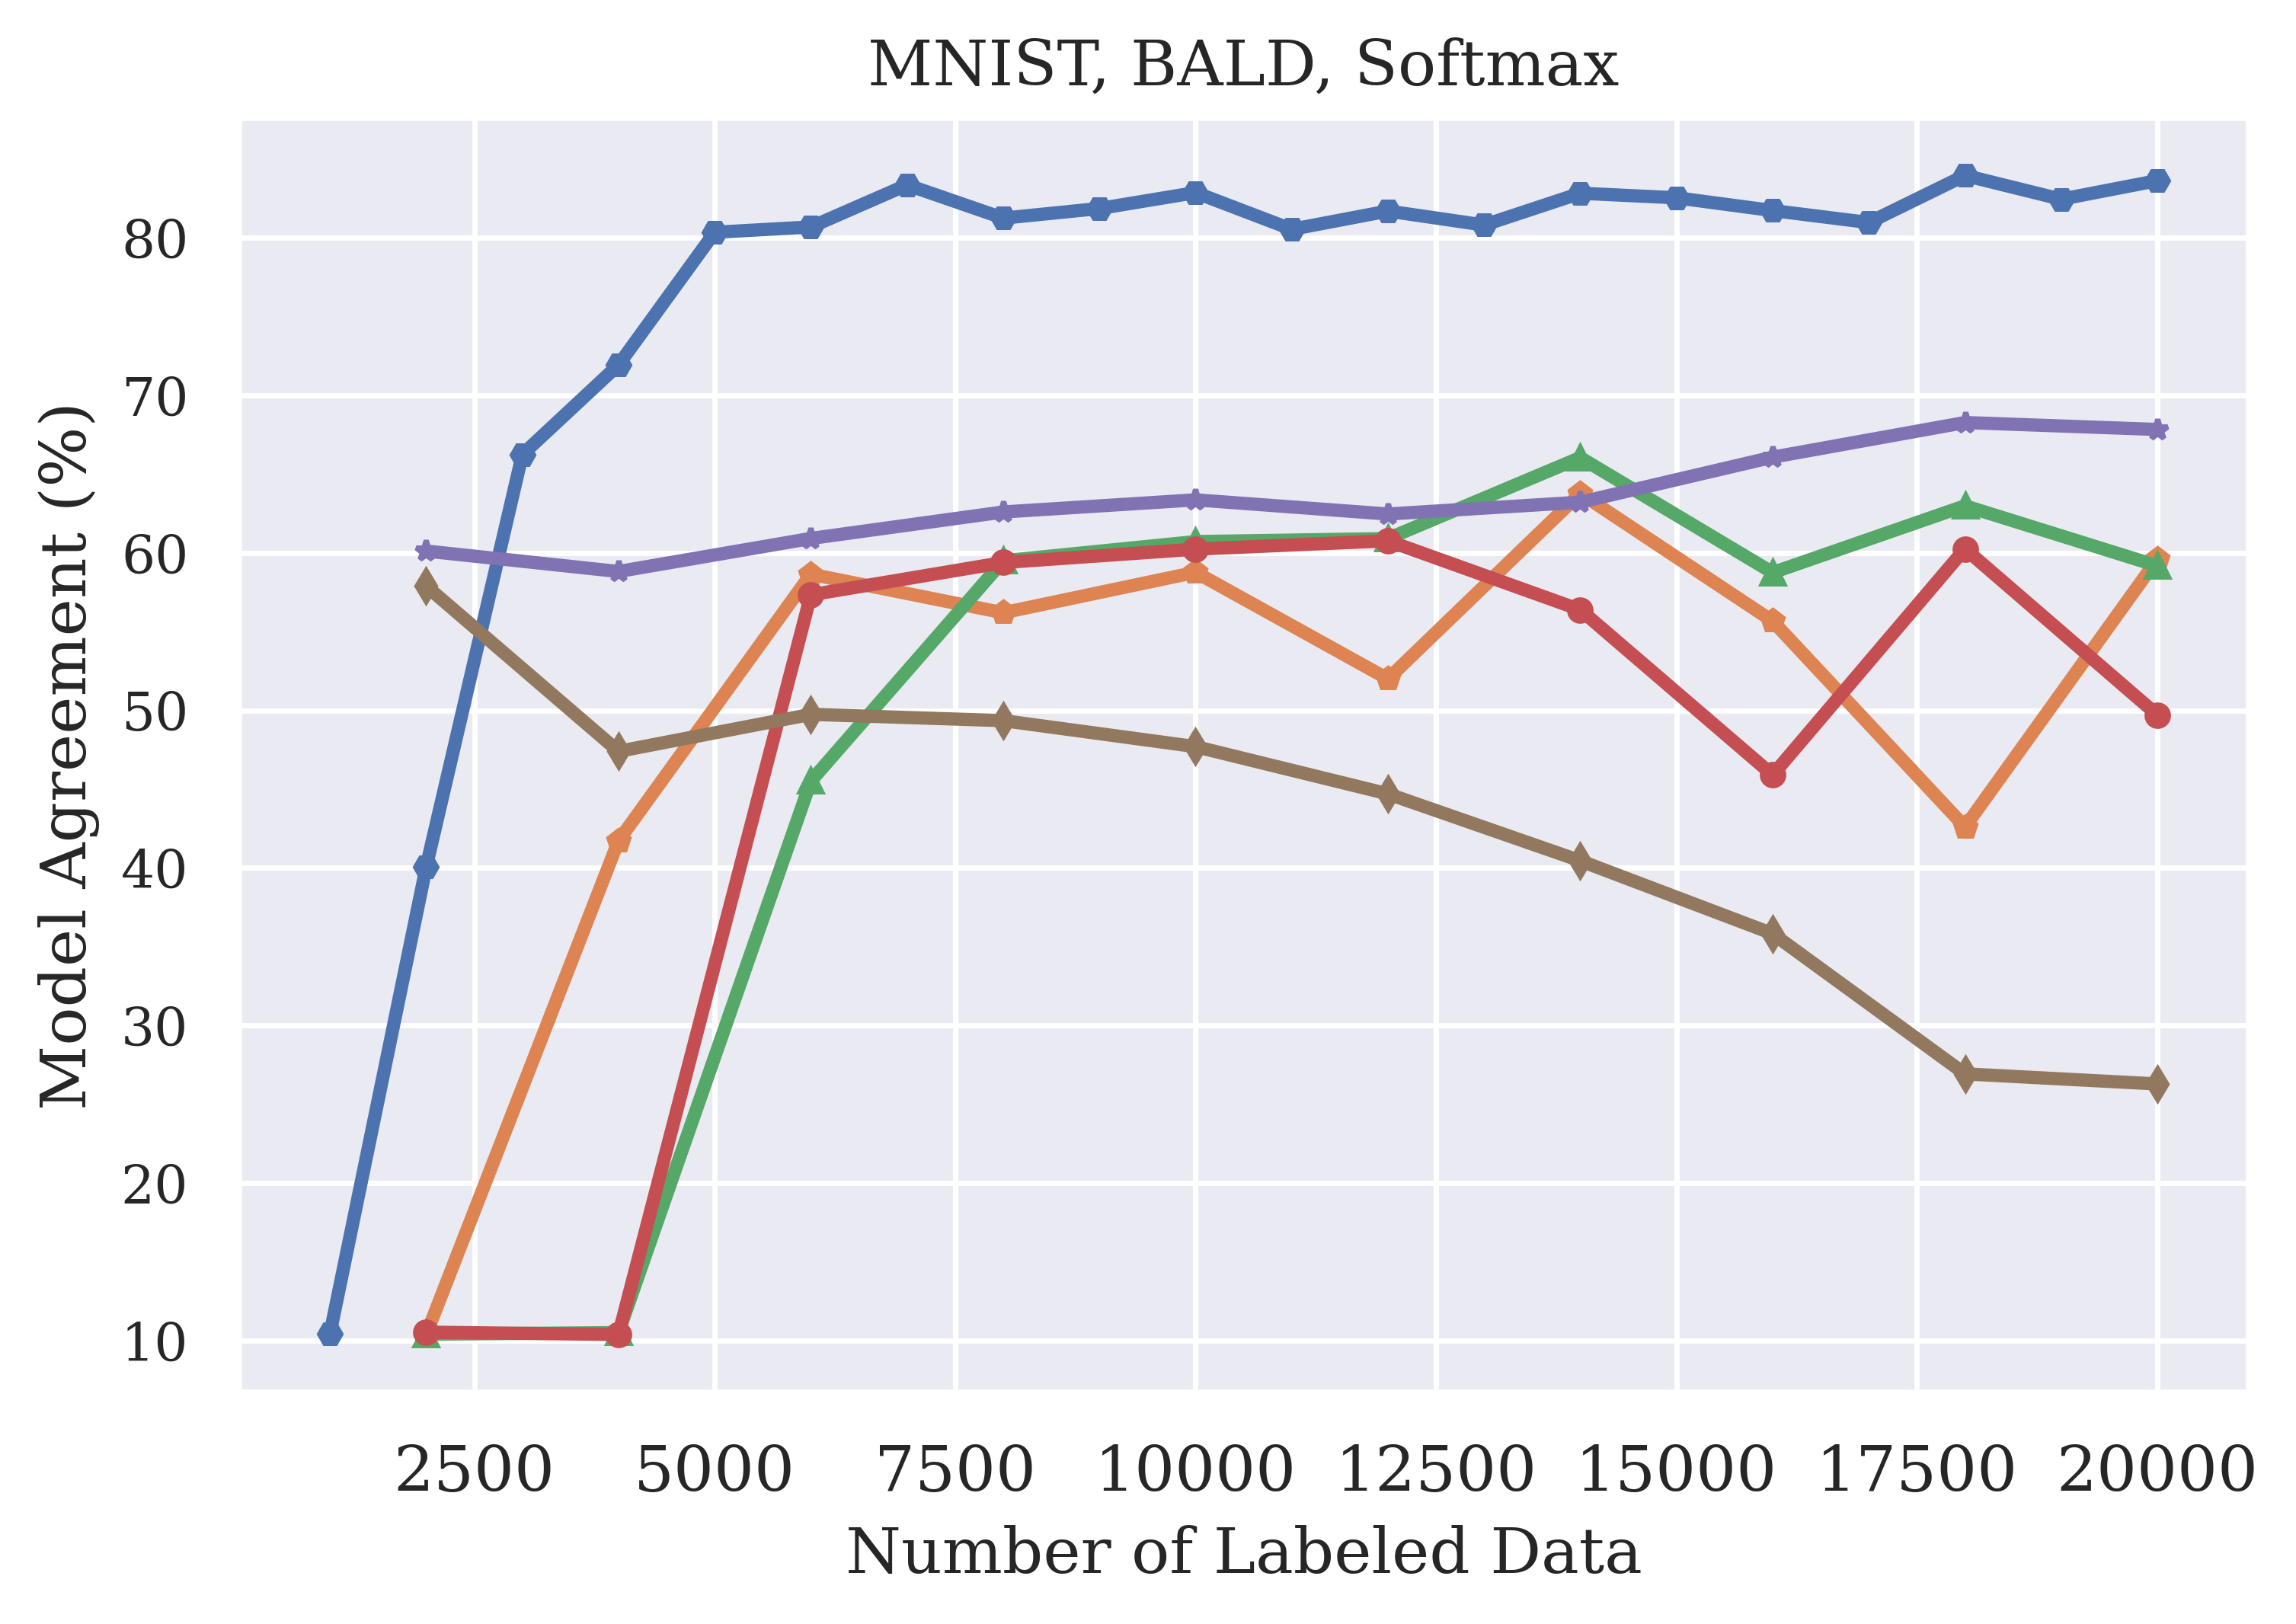
\includegraphics[width=0.48\linewidth]{images/results_CALMS/mnist_softmax_bald.png}
    \caption{Agreement comparison for model stealing on MNIST using the active learning strategy \gls{bald}.}
    \label{fig:CALMSMNISTBALD}
\end{figure}

\begin{figure}[!htb]
    \centering
    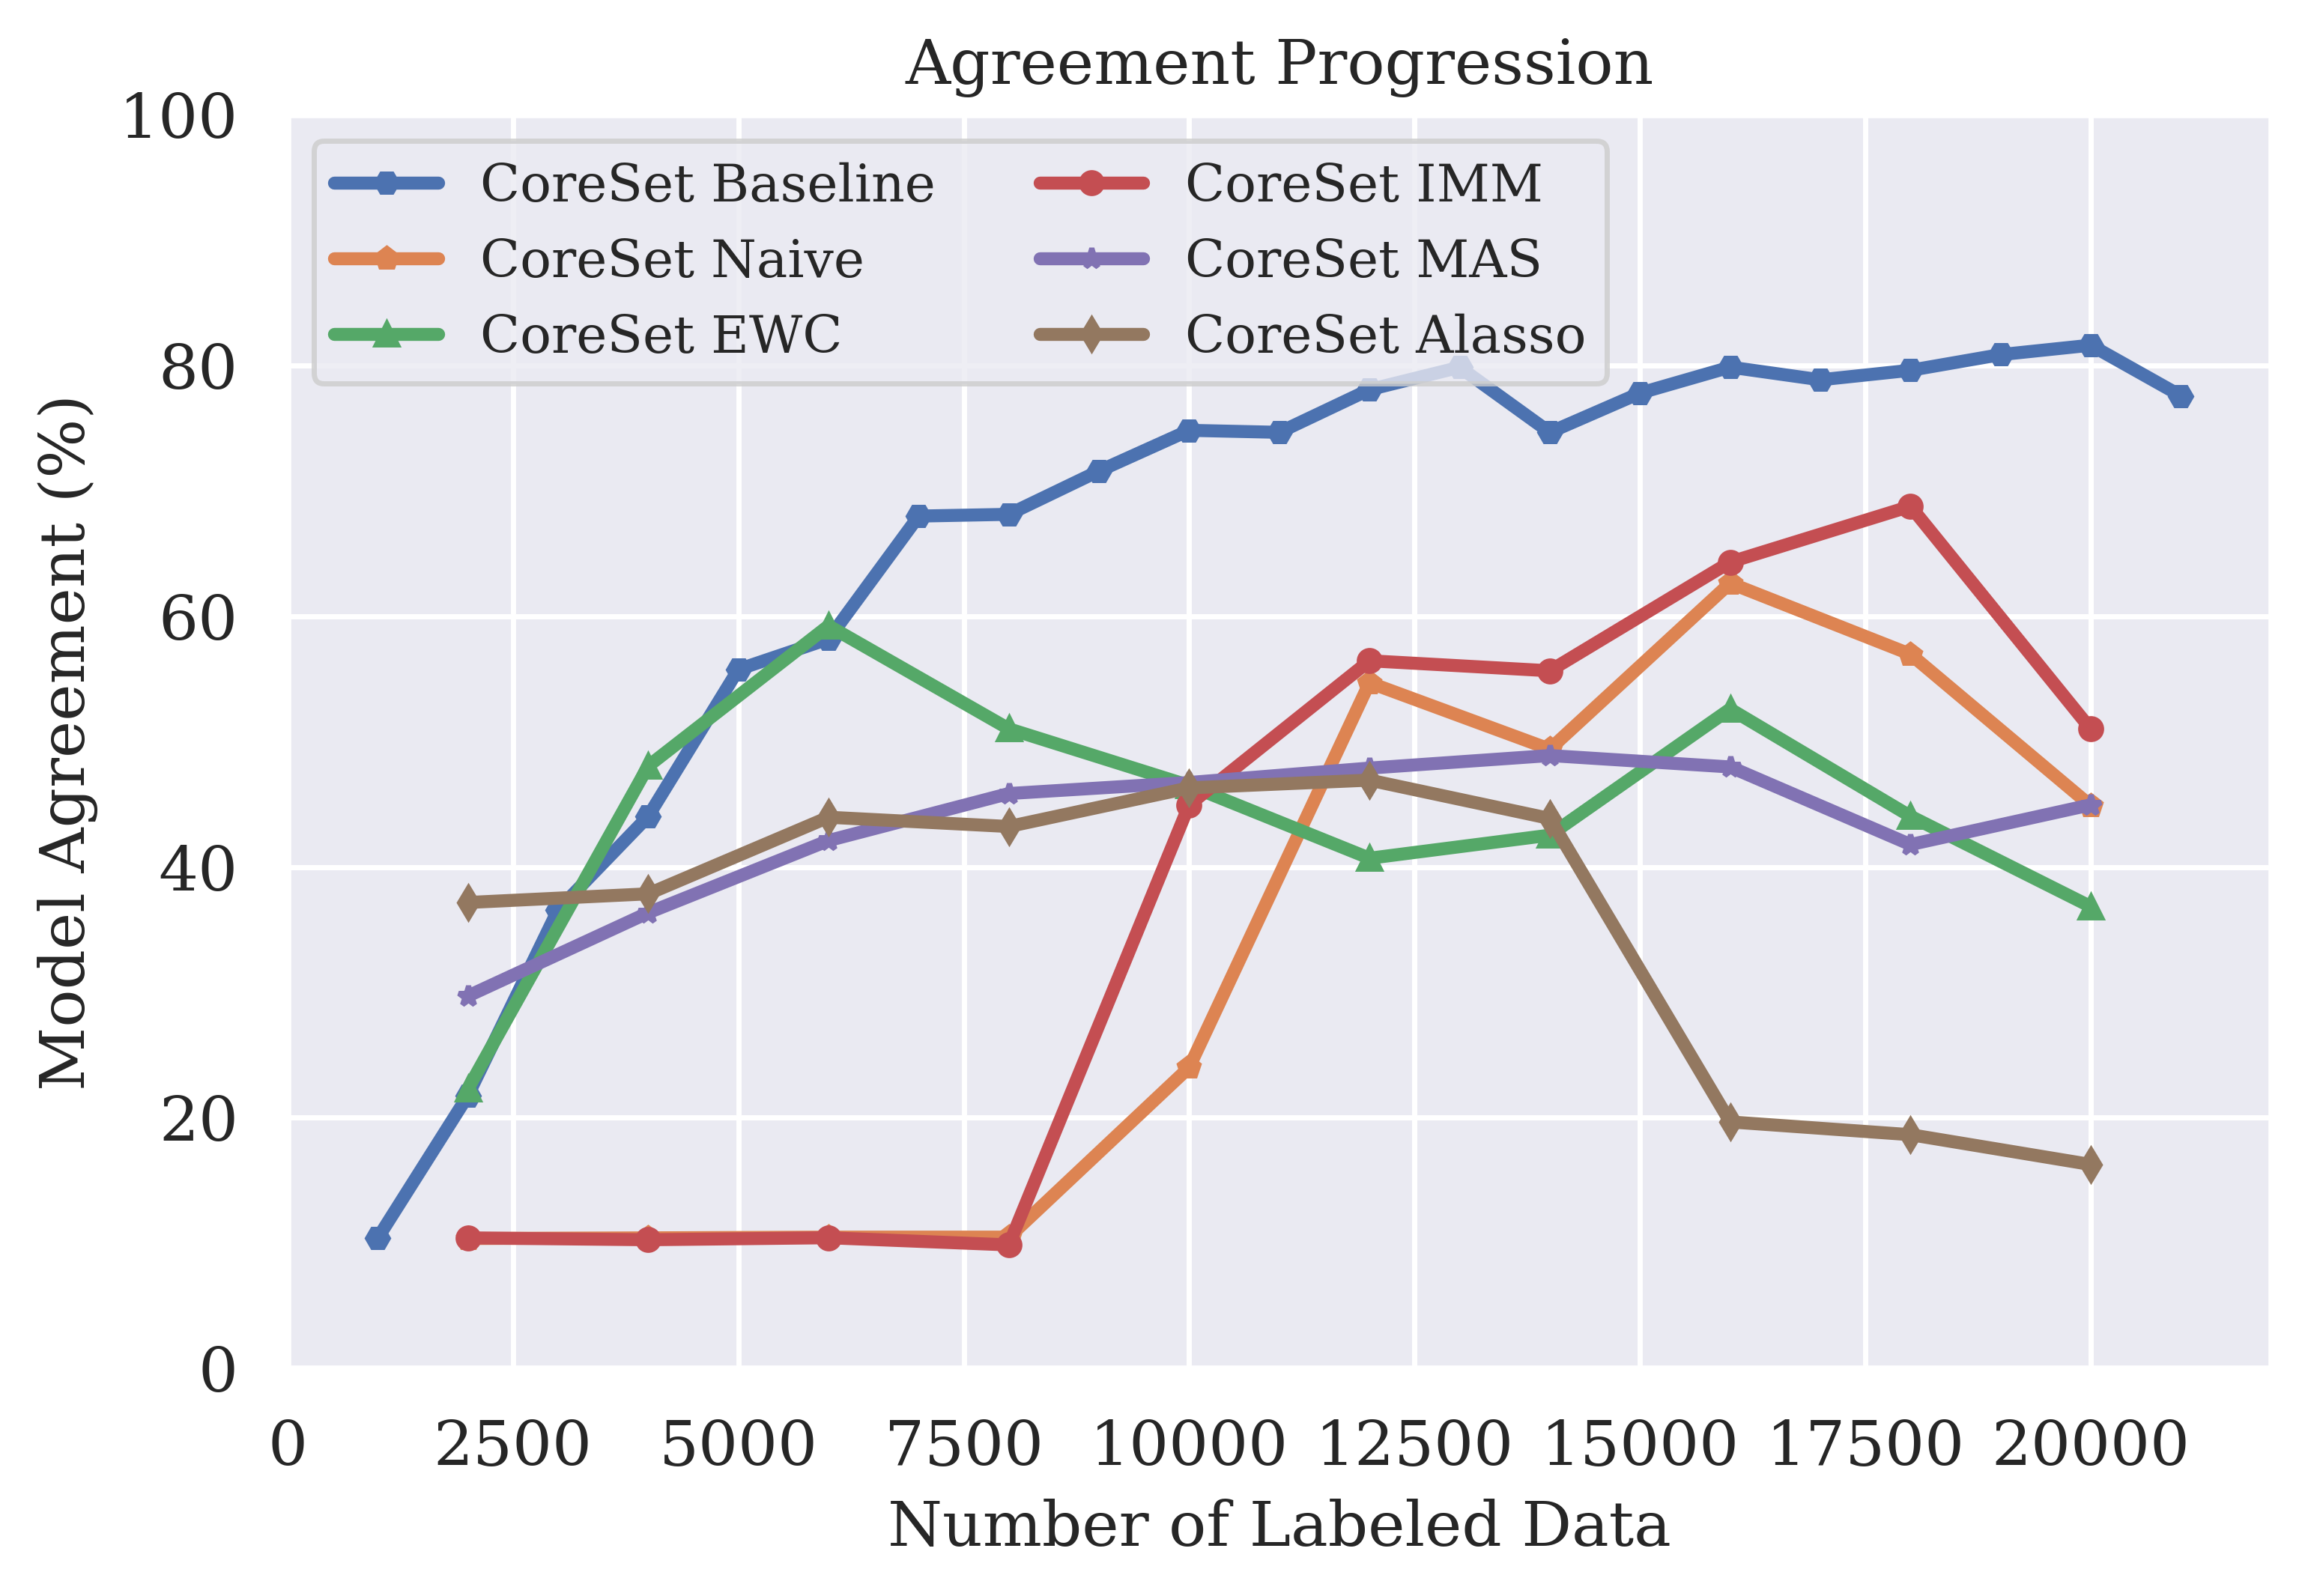
\includegraphics[width=0.48\linewidth]{images/results_CALMS/mnist_label_coreset.png} \hfill
    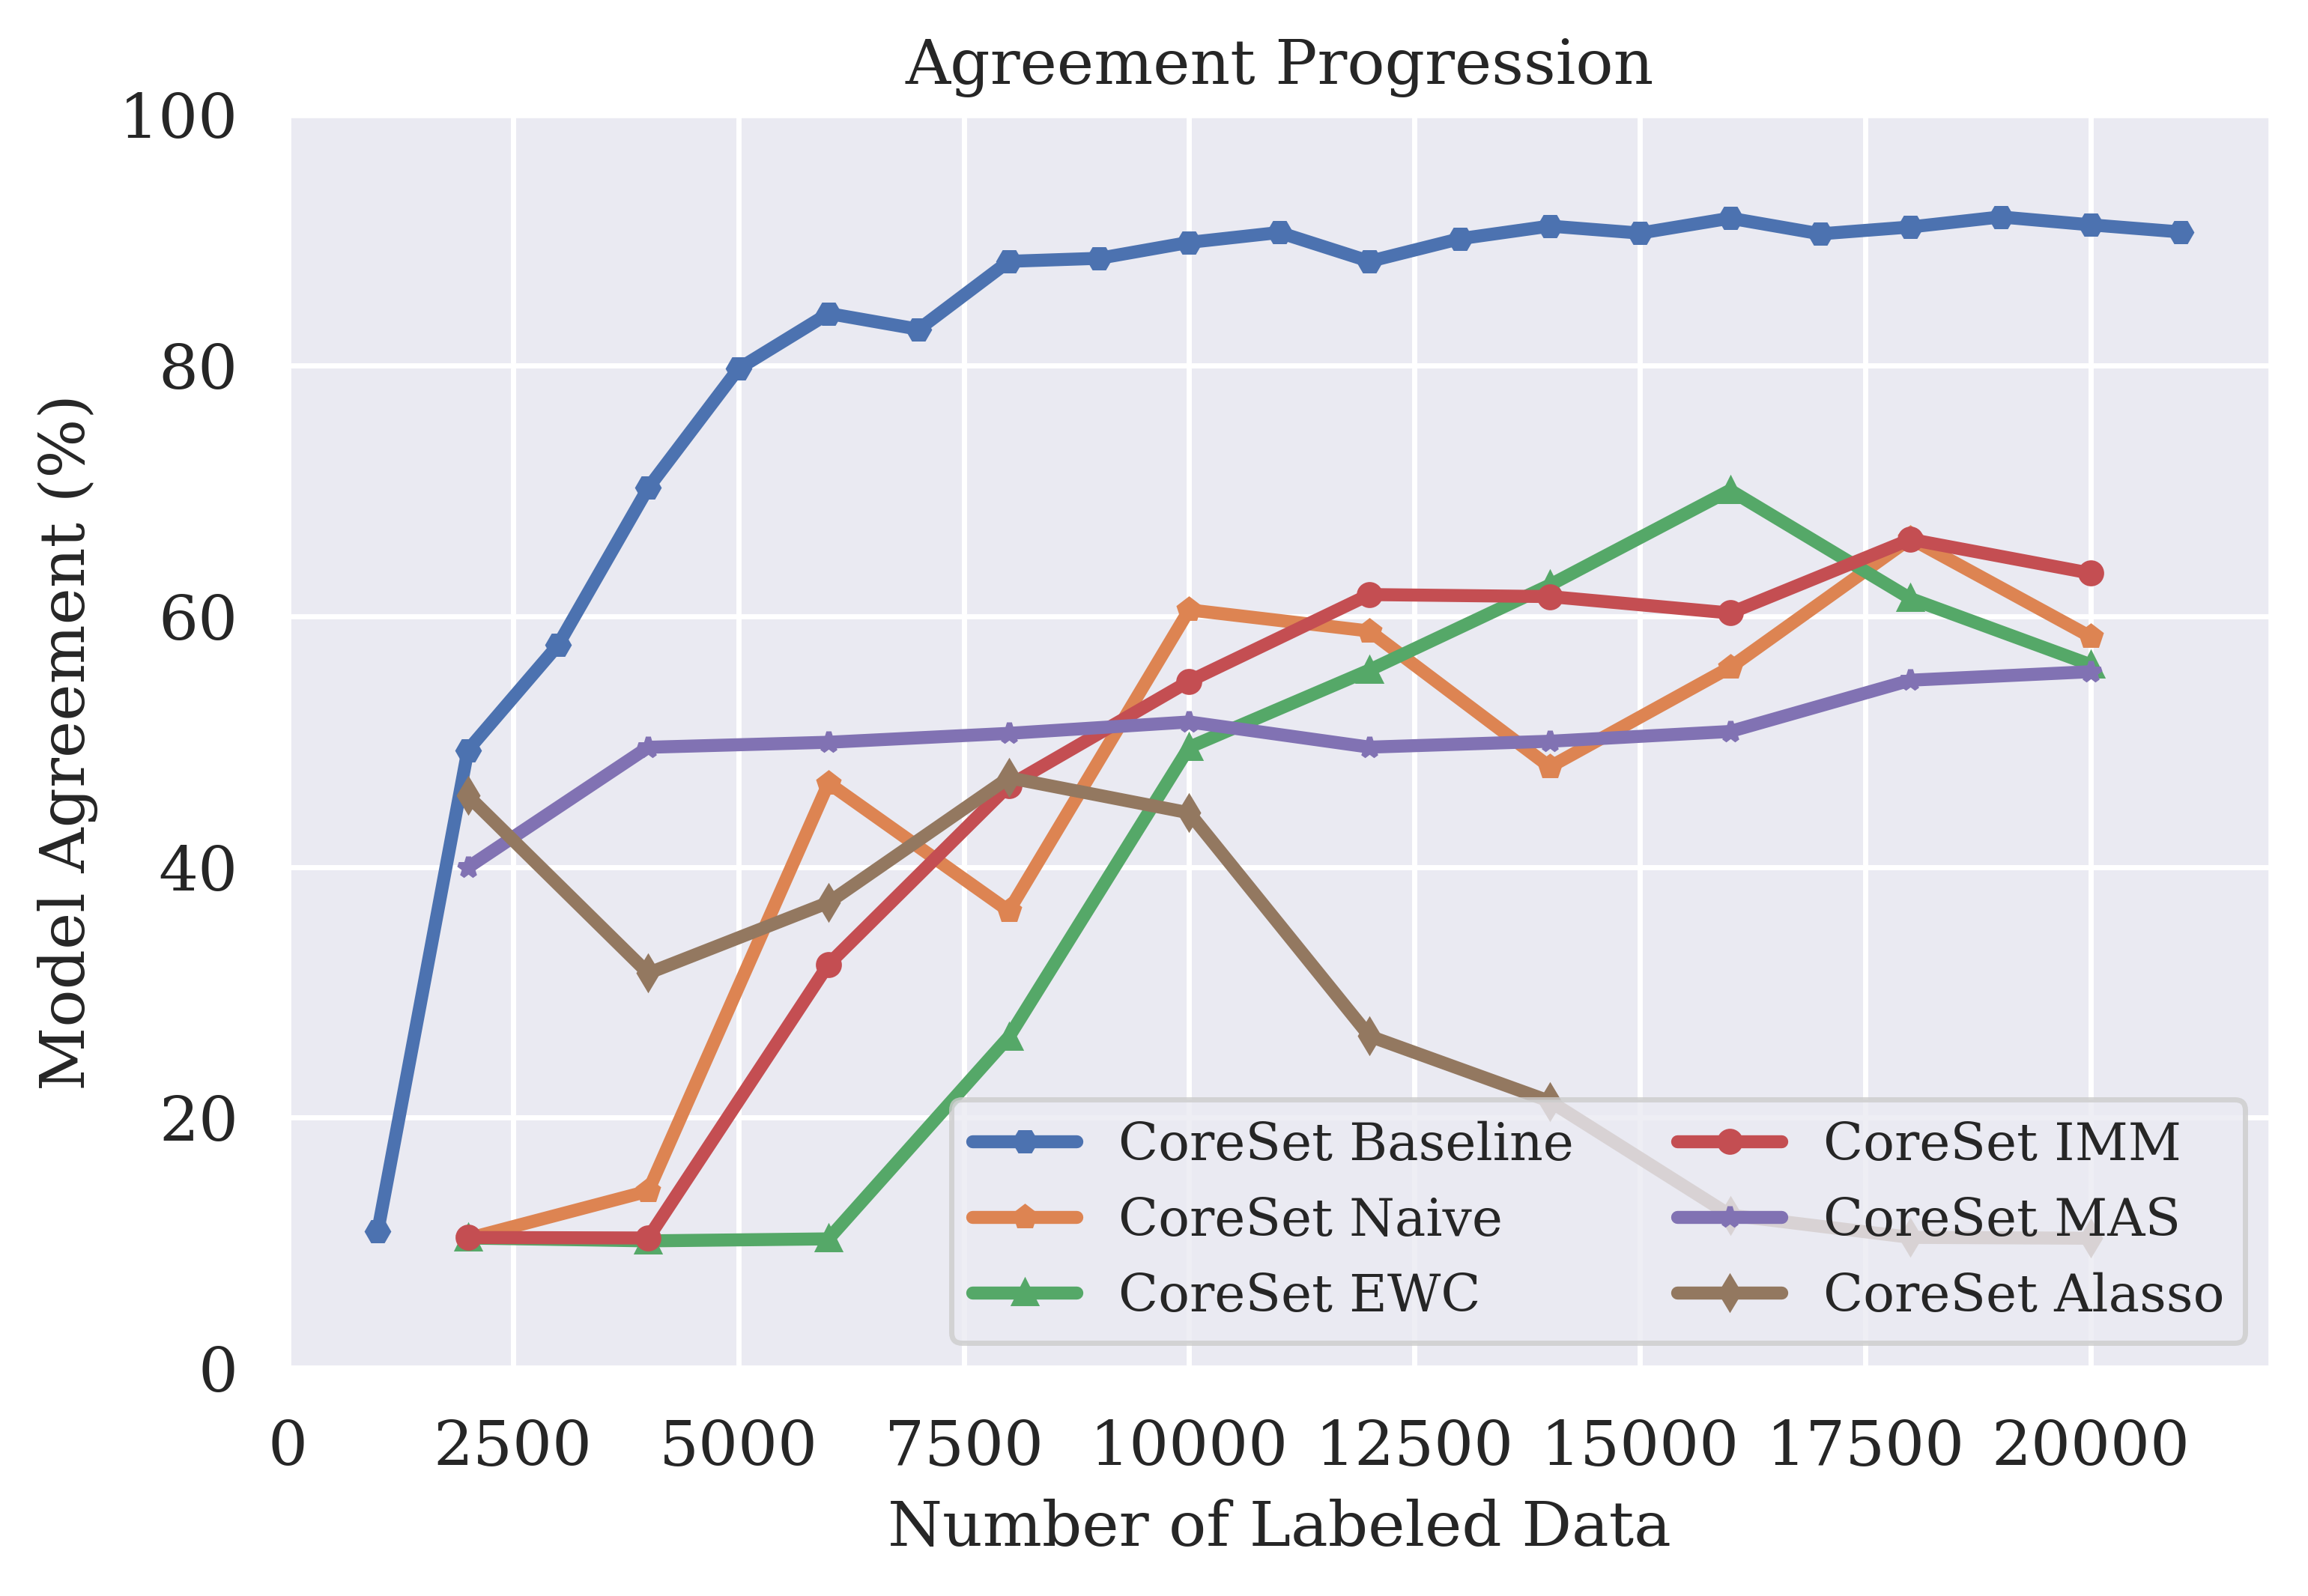
\includegraphics[width=0.48\linewidth]{images/results_CALMS/mnist_softmax_coreset.png}
    \caption{Agreement comparison for model stealing on MNIST using the active learning strategy CoreSet.}
    \label{fig:CALMSMNISTCoreSet}
\end{figure}

\begin{figure}[!htb]
    \centering
    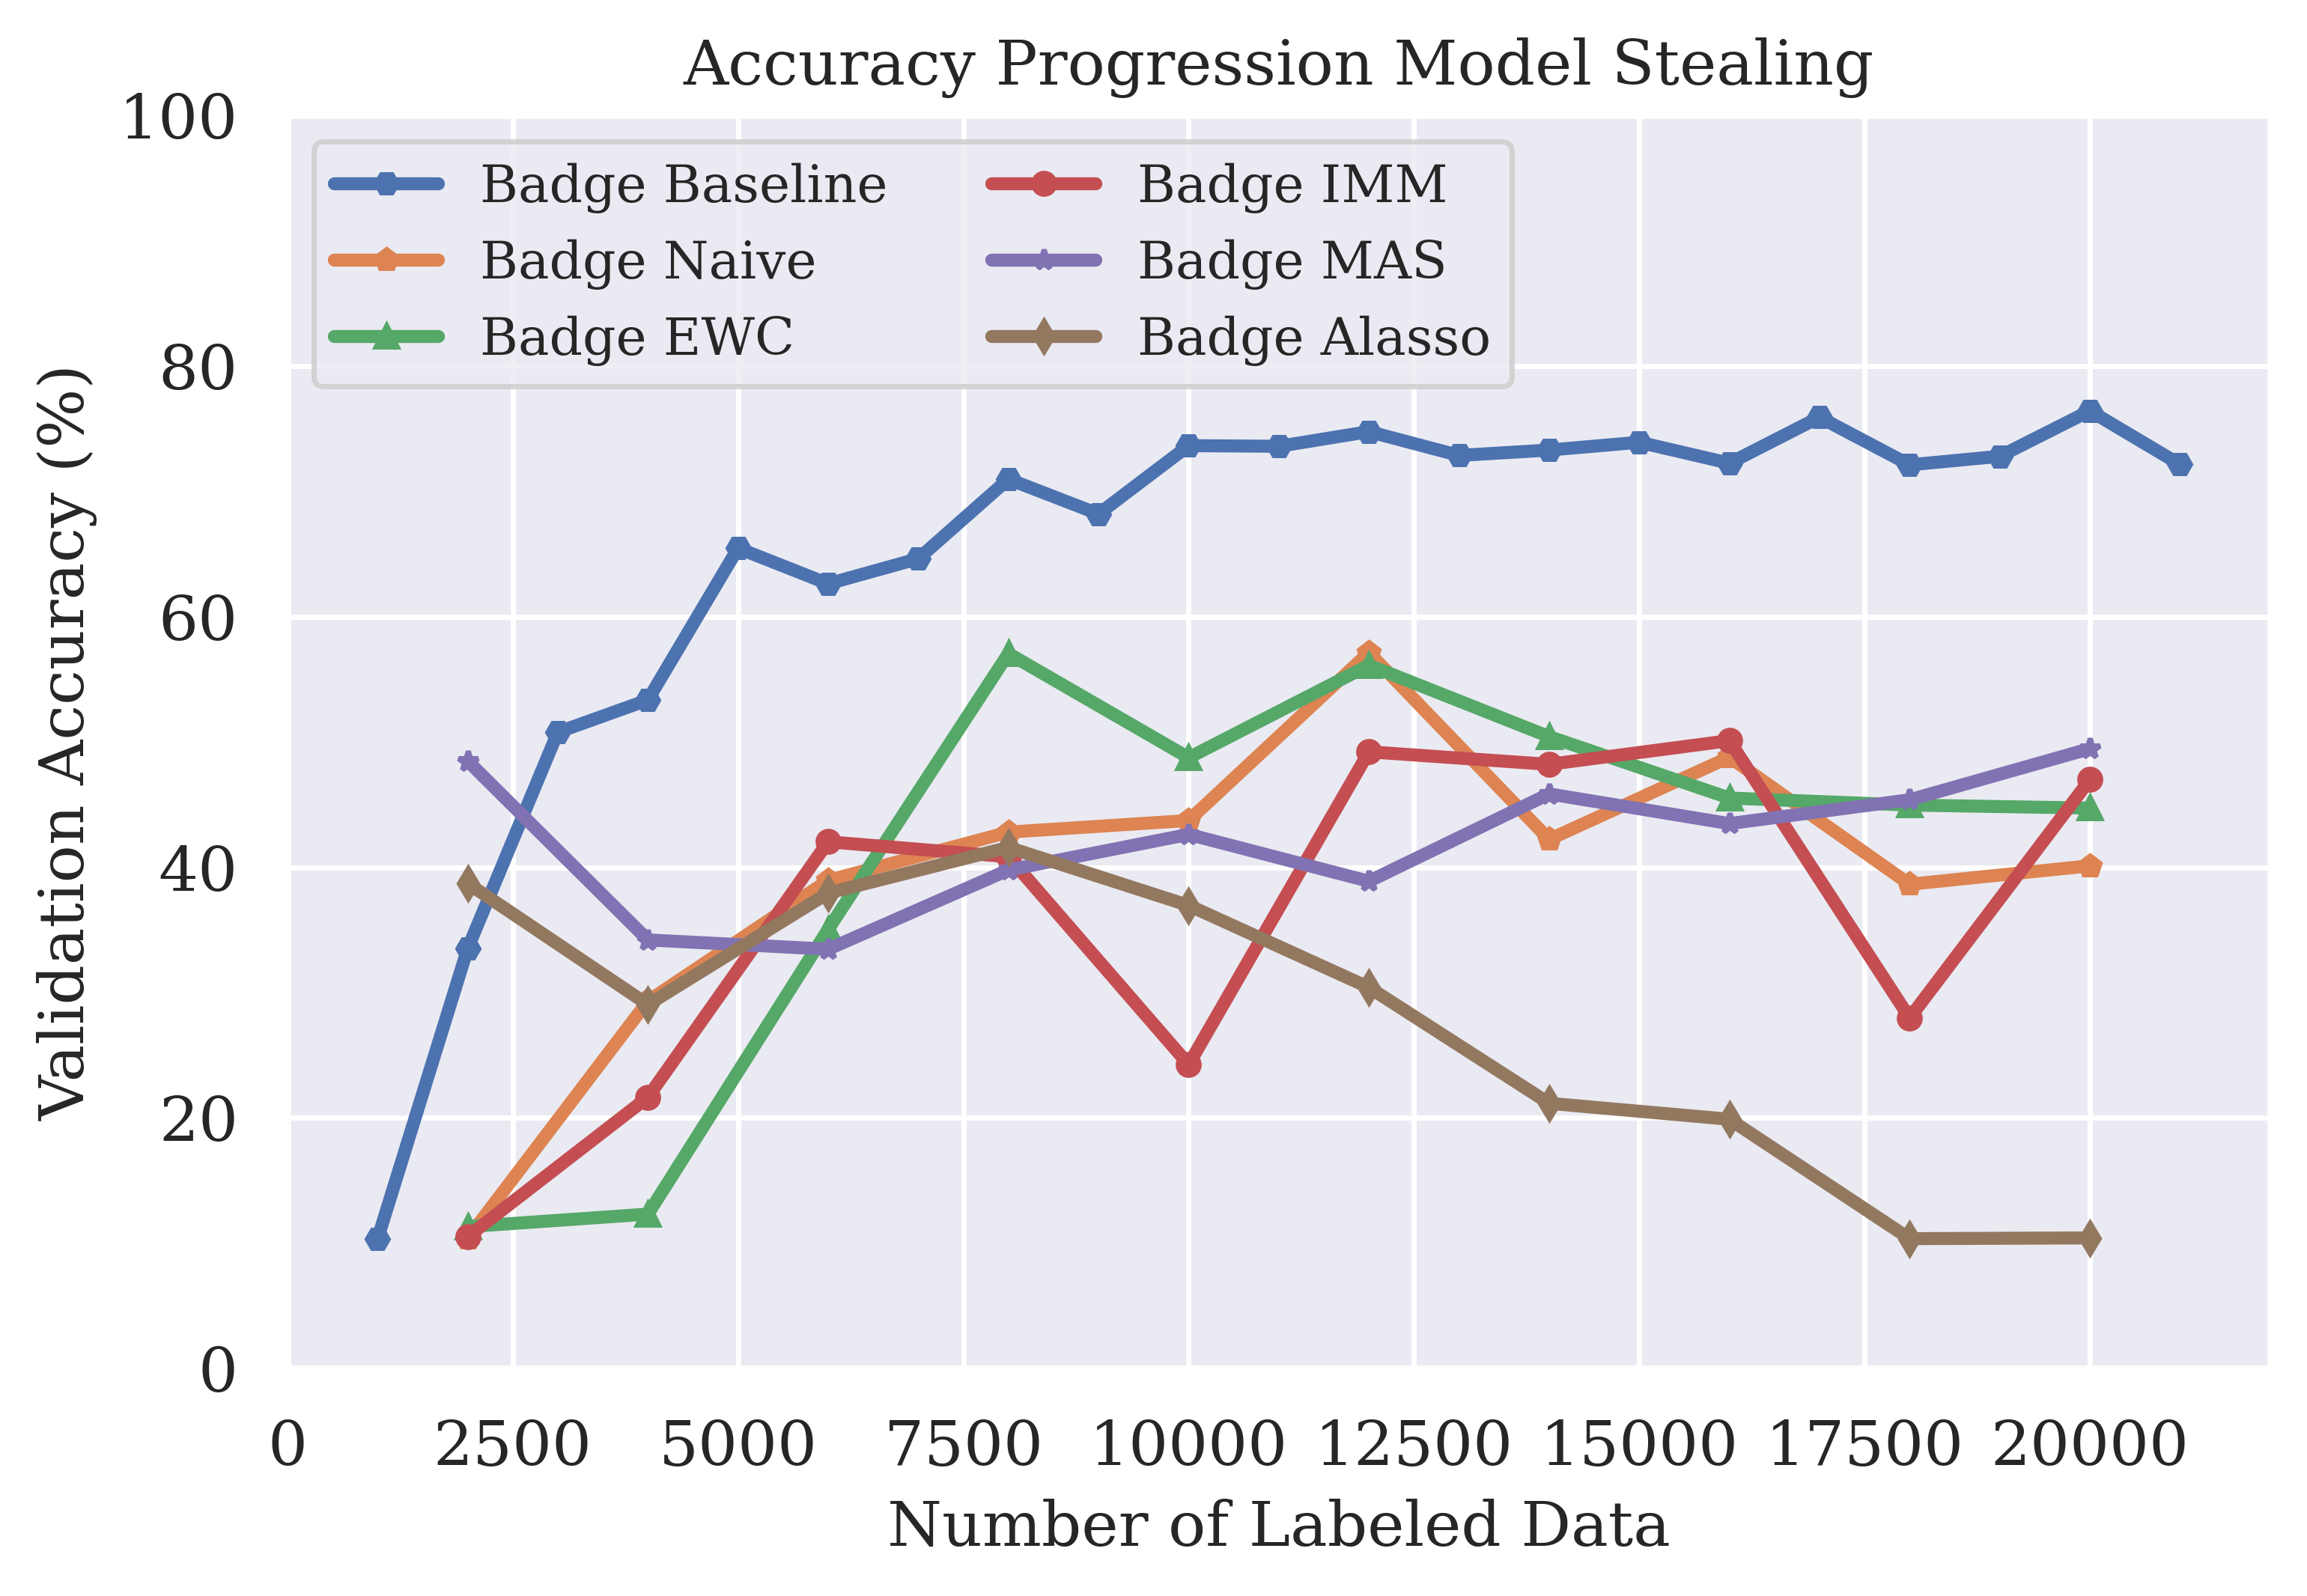
\includegraphics[width=0.48\linewidth]{images/results_CALMS/mnist_label_badge.png} \hfill
    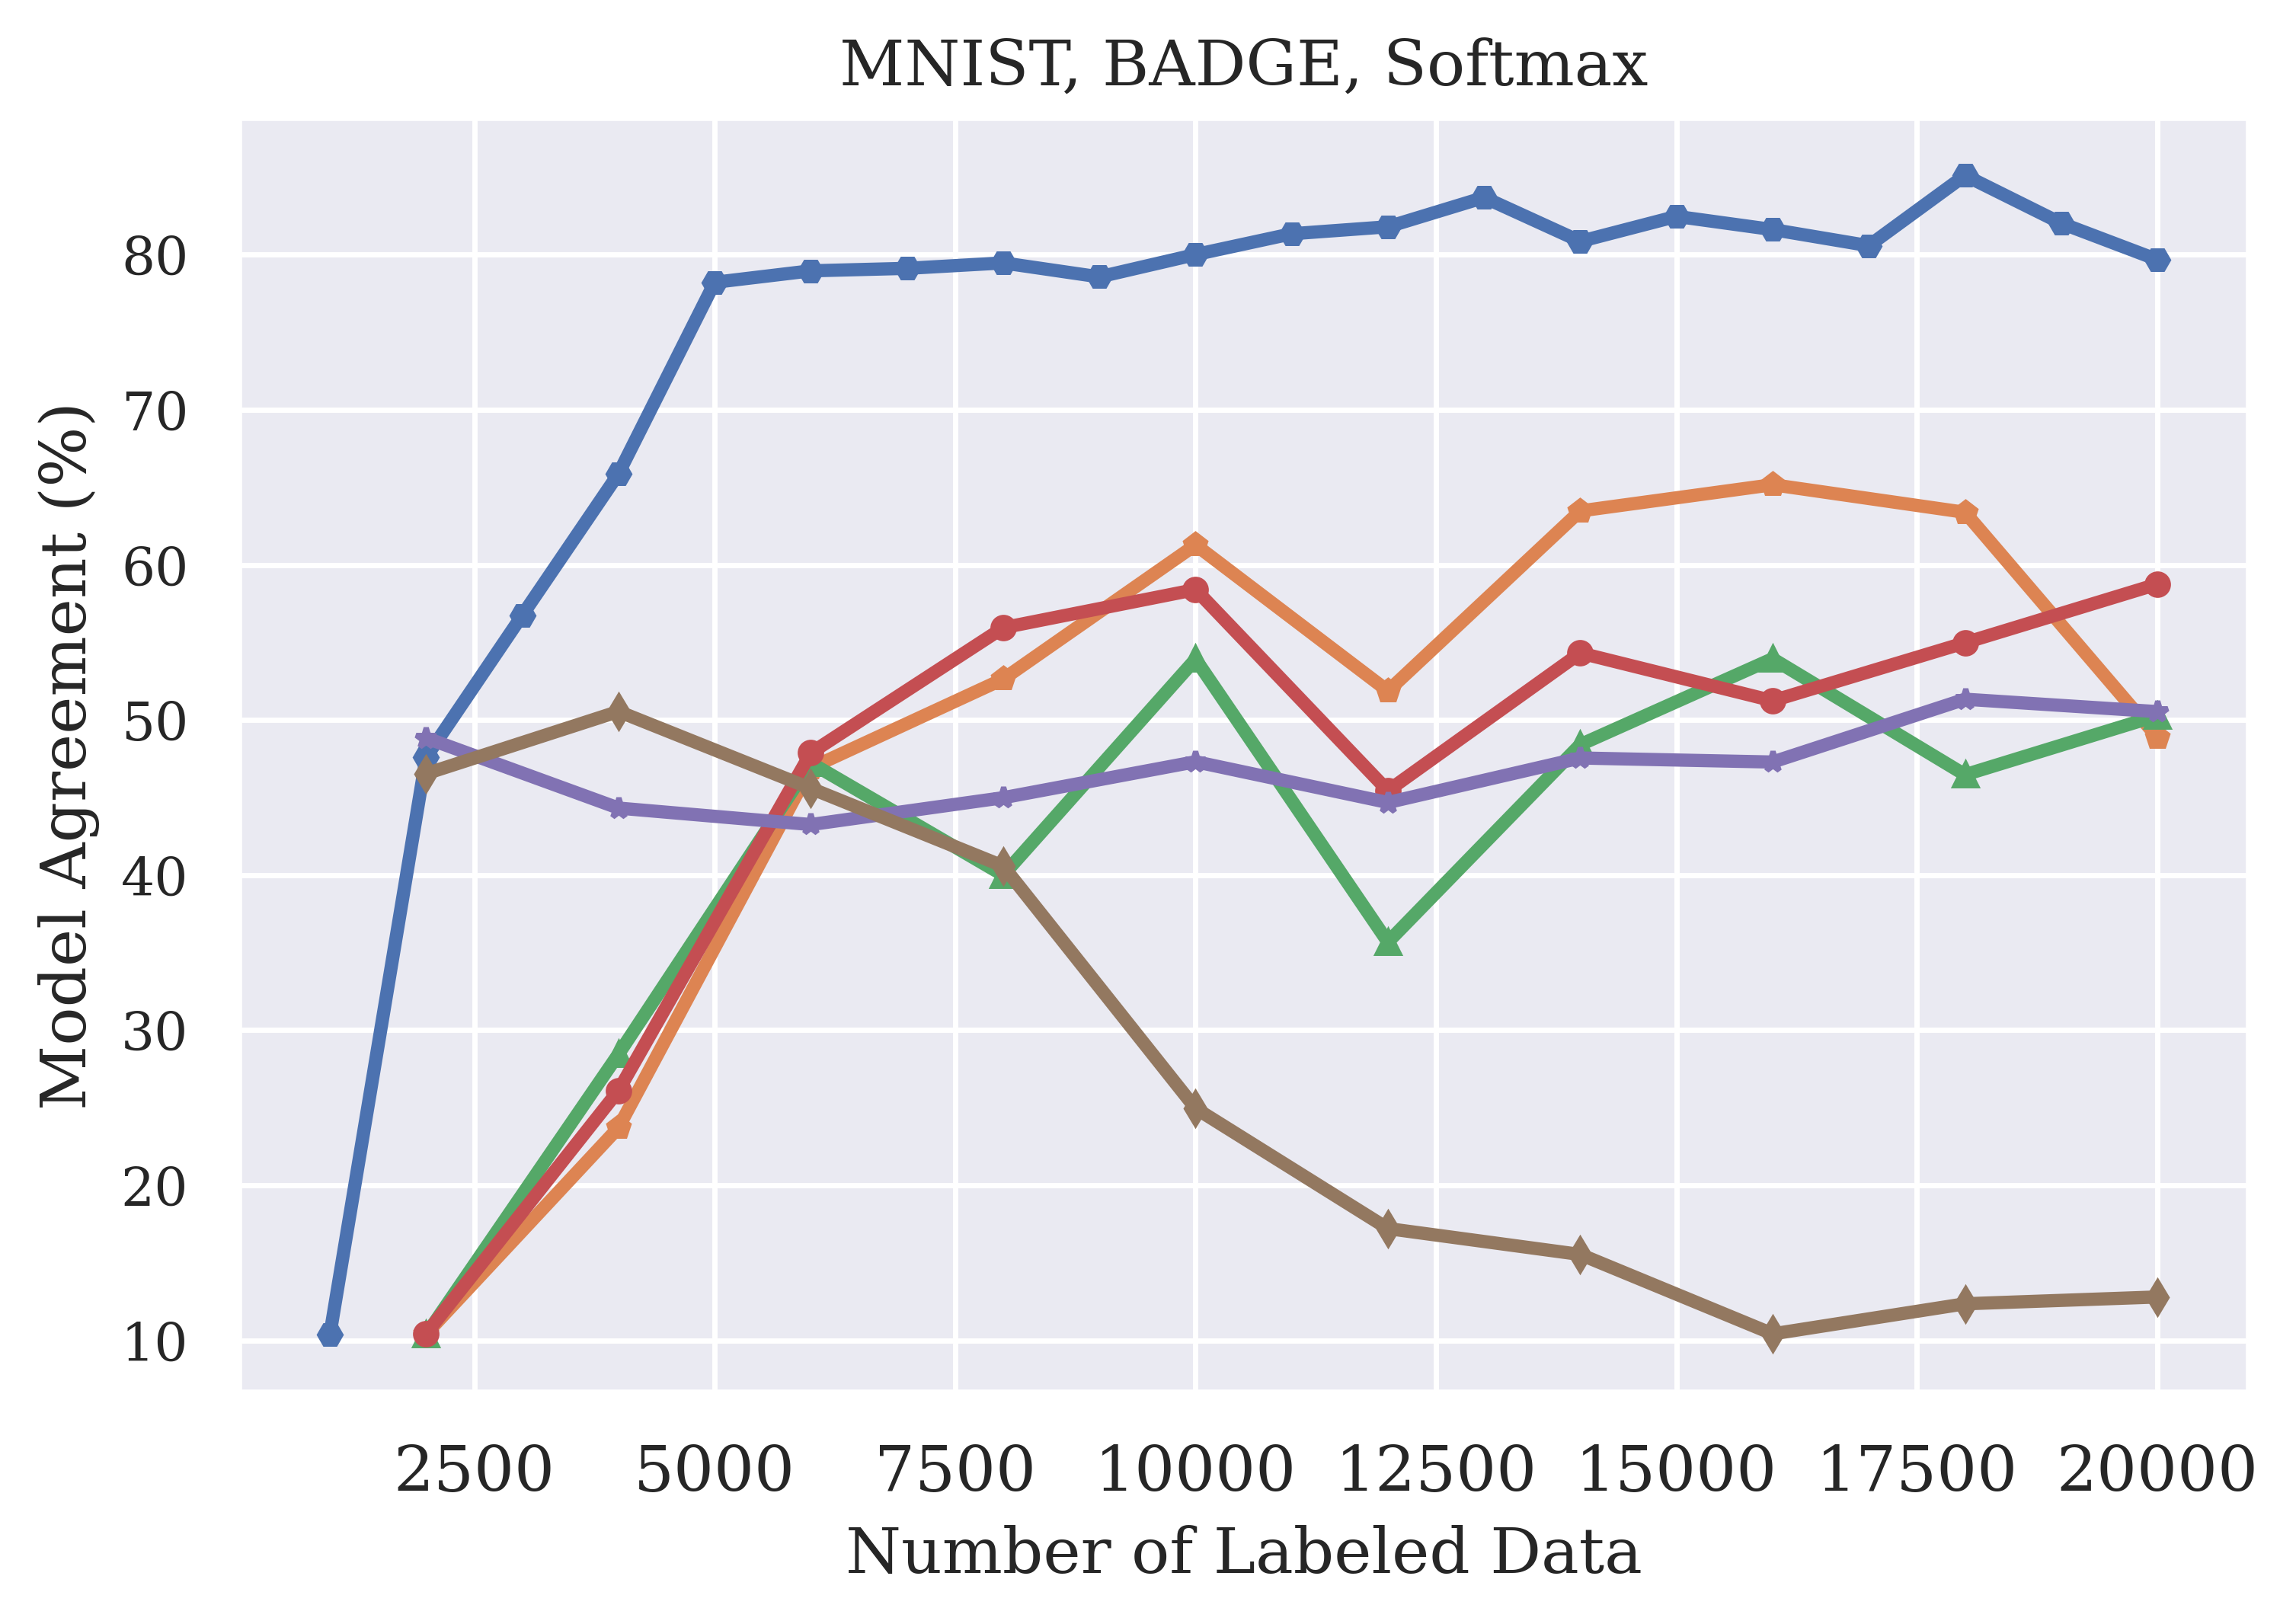
\includegraphics[width=0.48\linewidth]{images/results_CALMS/mnist_softmax_badge.png}
    \caption{Agreement comparison for model stealing on MNIST using the active learning strategy \gls{badge}.}
    \label{fig:CALMSMNISTBadge}
\end{figure}

\clearpage

\subsubsection{CIFAR-10}
\label{sec:Appendix:CALMS:CIFAR}
In this section, we present the complete runs of all experiments which involve continual active learning using CIFAR-10 as a target model dataset.

\begin{figure}[!htb]
    \centering
    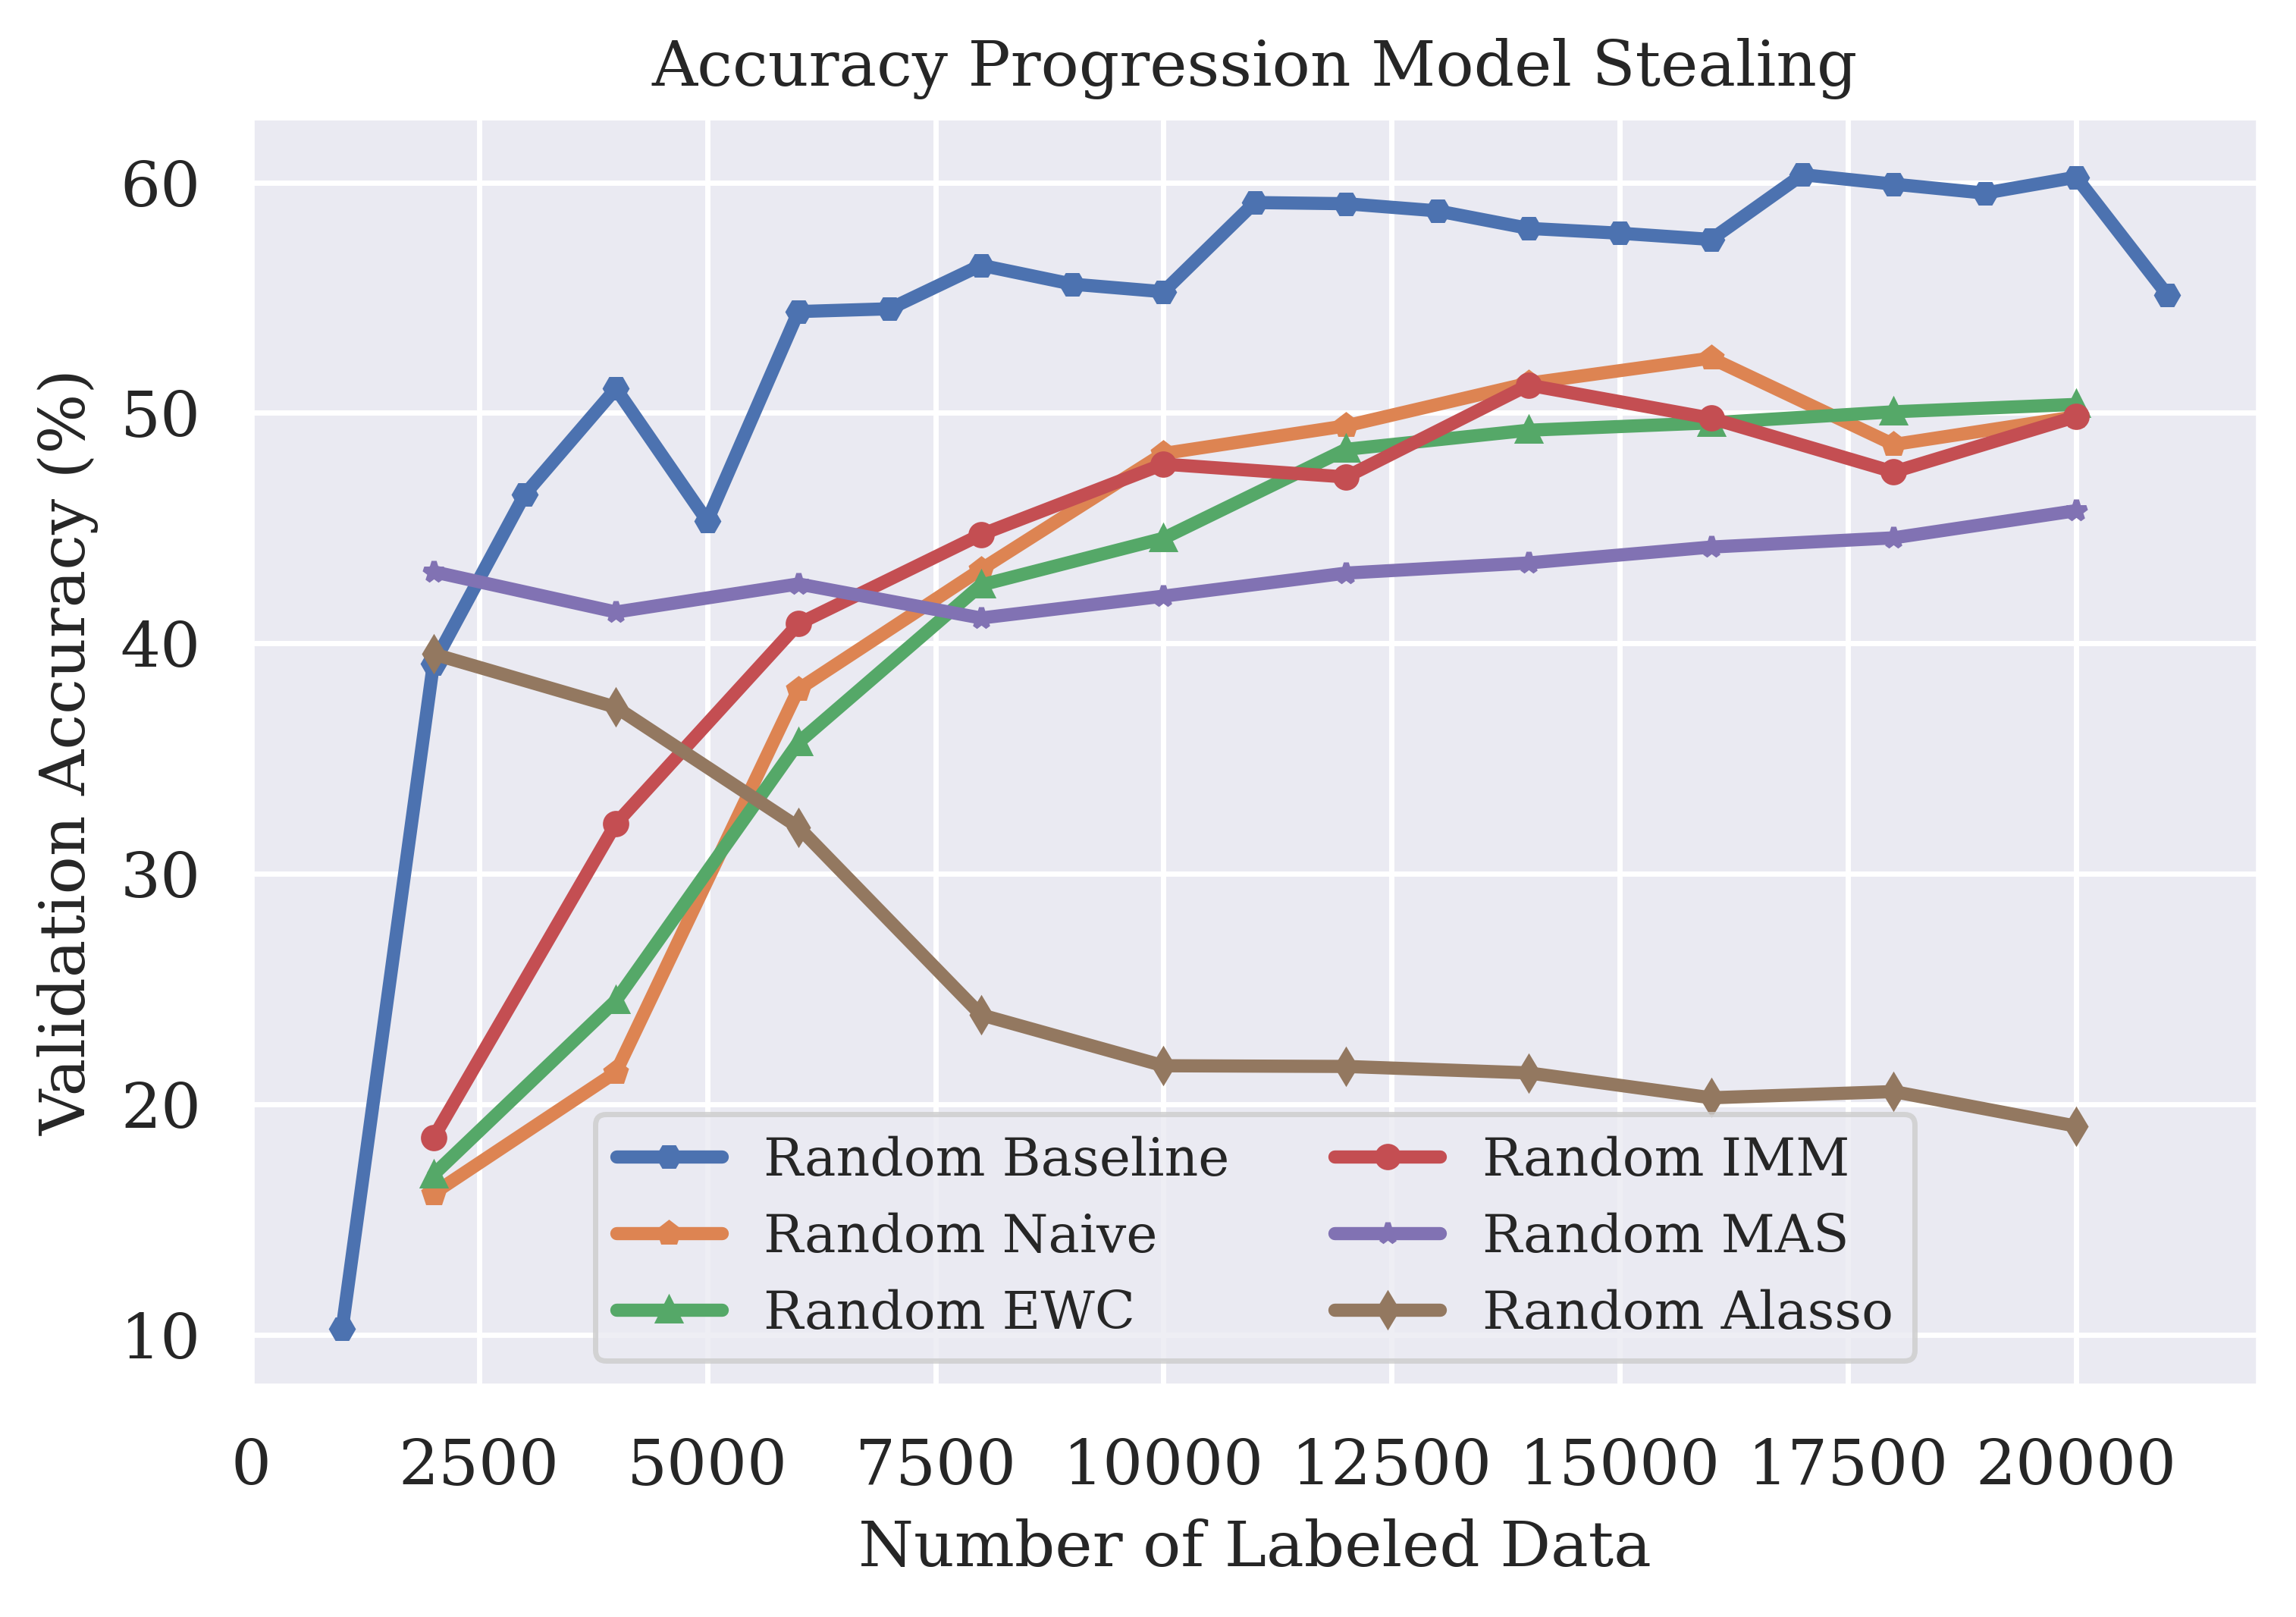
\includegraphics[width=0.48\linewidth]{images/results_CALMS/cifar_label_random.png} \hfill
    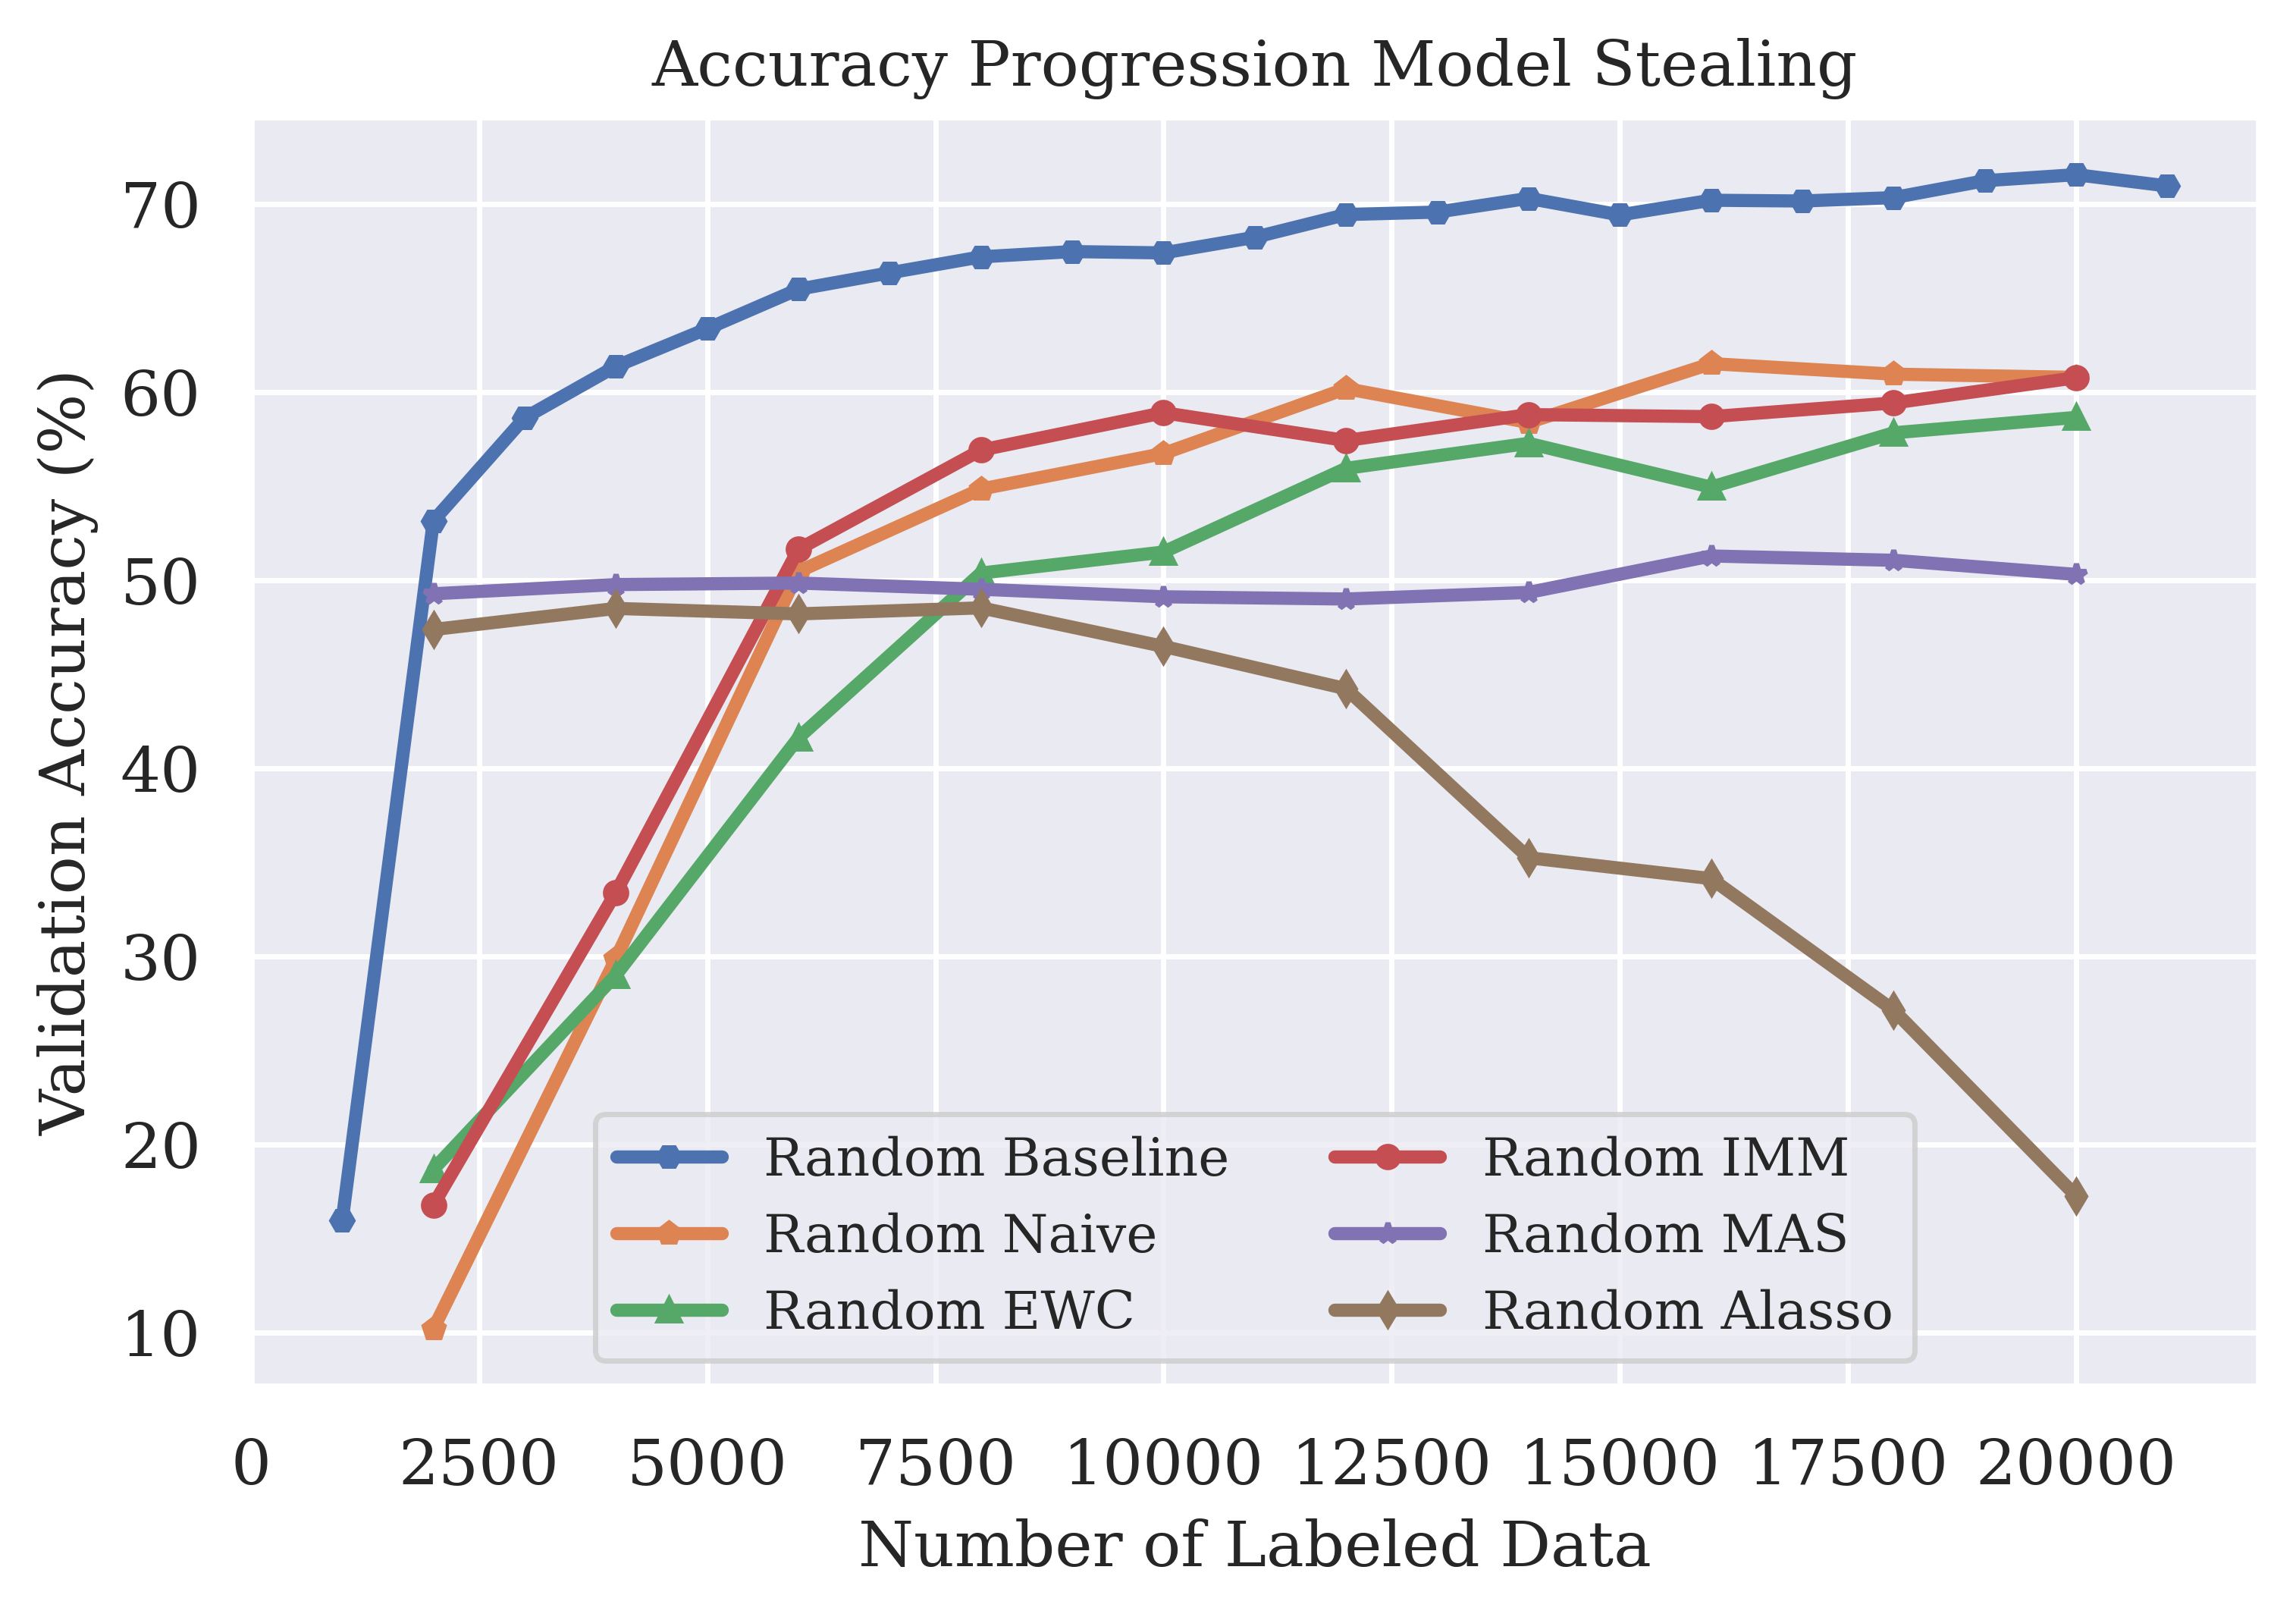
\includegraphics[width=0.48\linewidth]{images/results_CALMS/cifar_softmax_random.png}
    \caption{Agreement comparison for model stealing on CIFAR-10 using the active learning strategy Random.}
    \label{fig:CALMSCIFAR10Random}
\end{figure}

\begin{figure}[!htb]
    \centering
    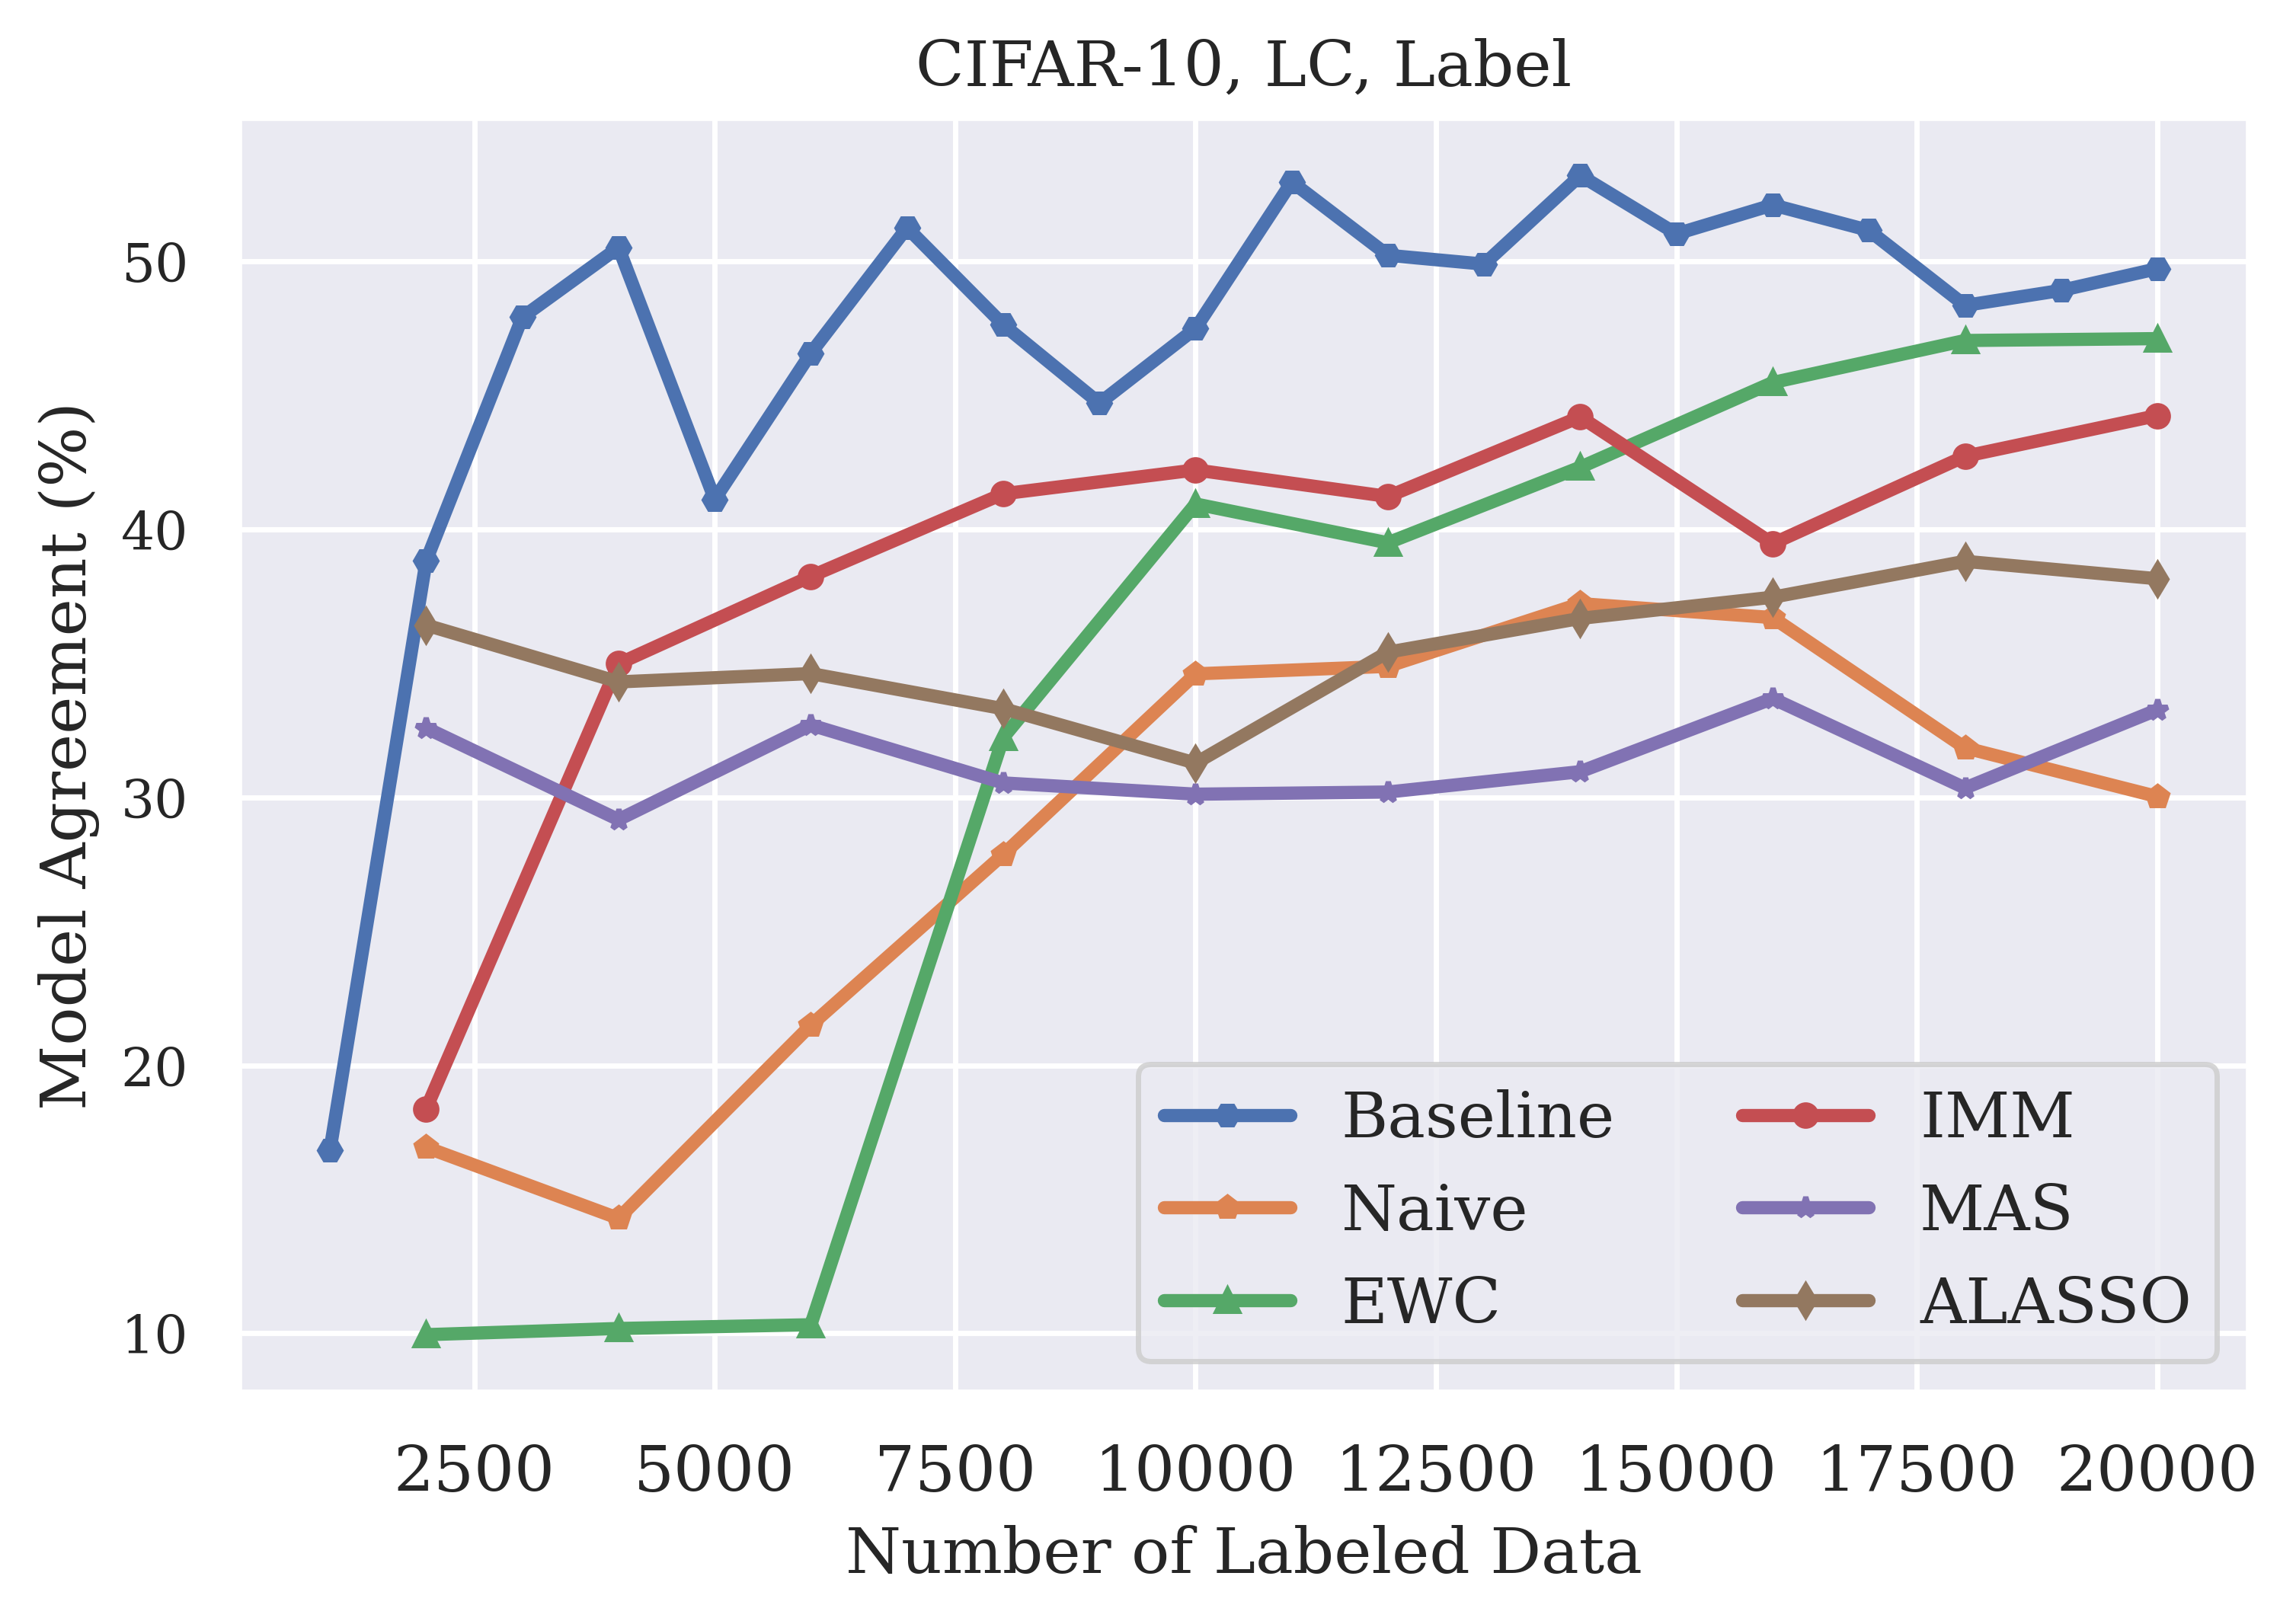
\includegraphics[width=0.48\linewidth]{images/results_CALMS/cifar_label_lc.png} \hfill
    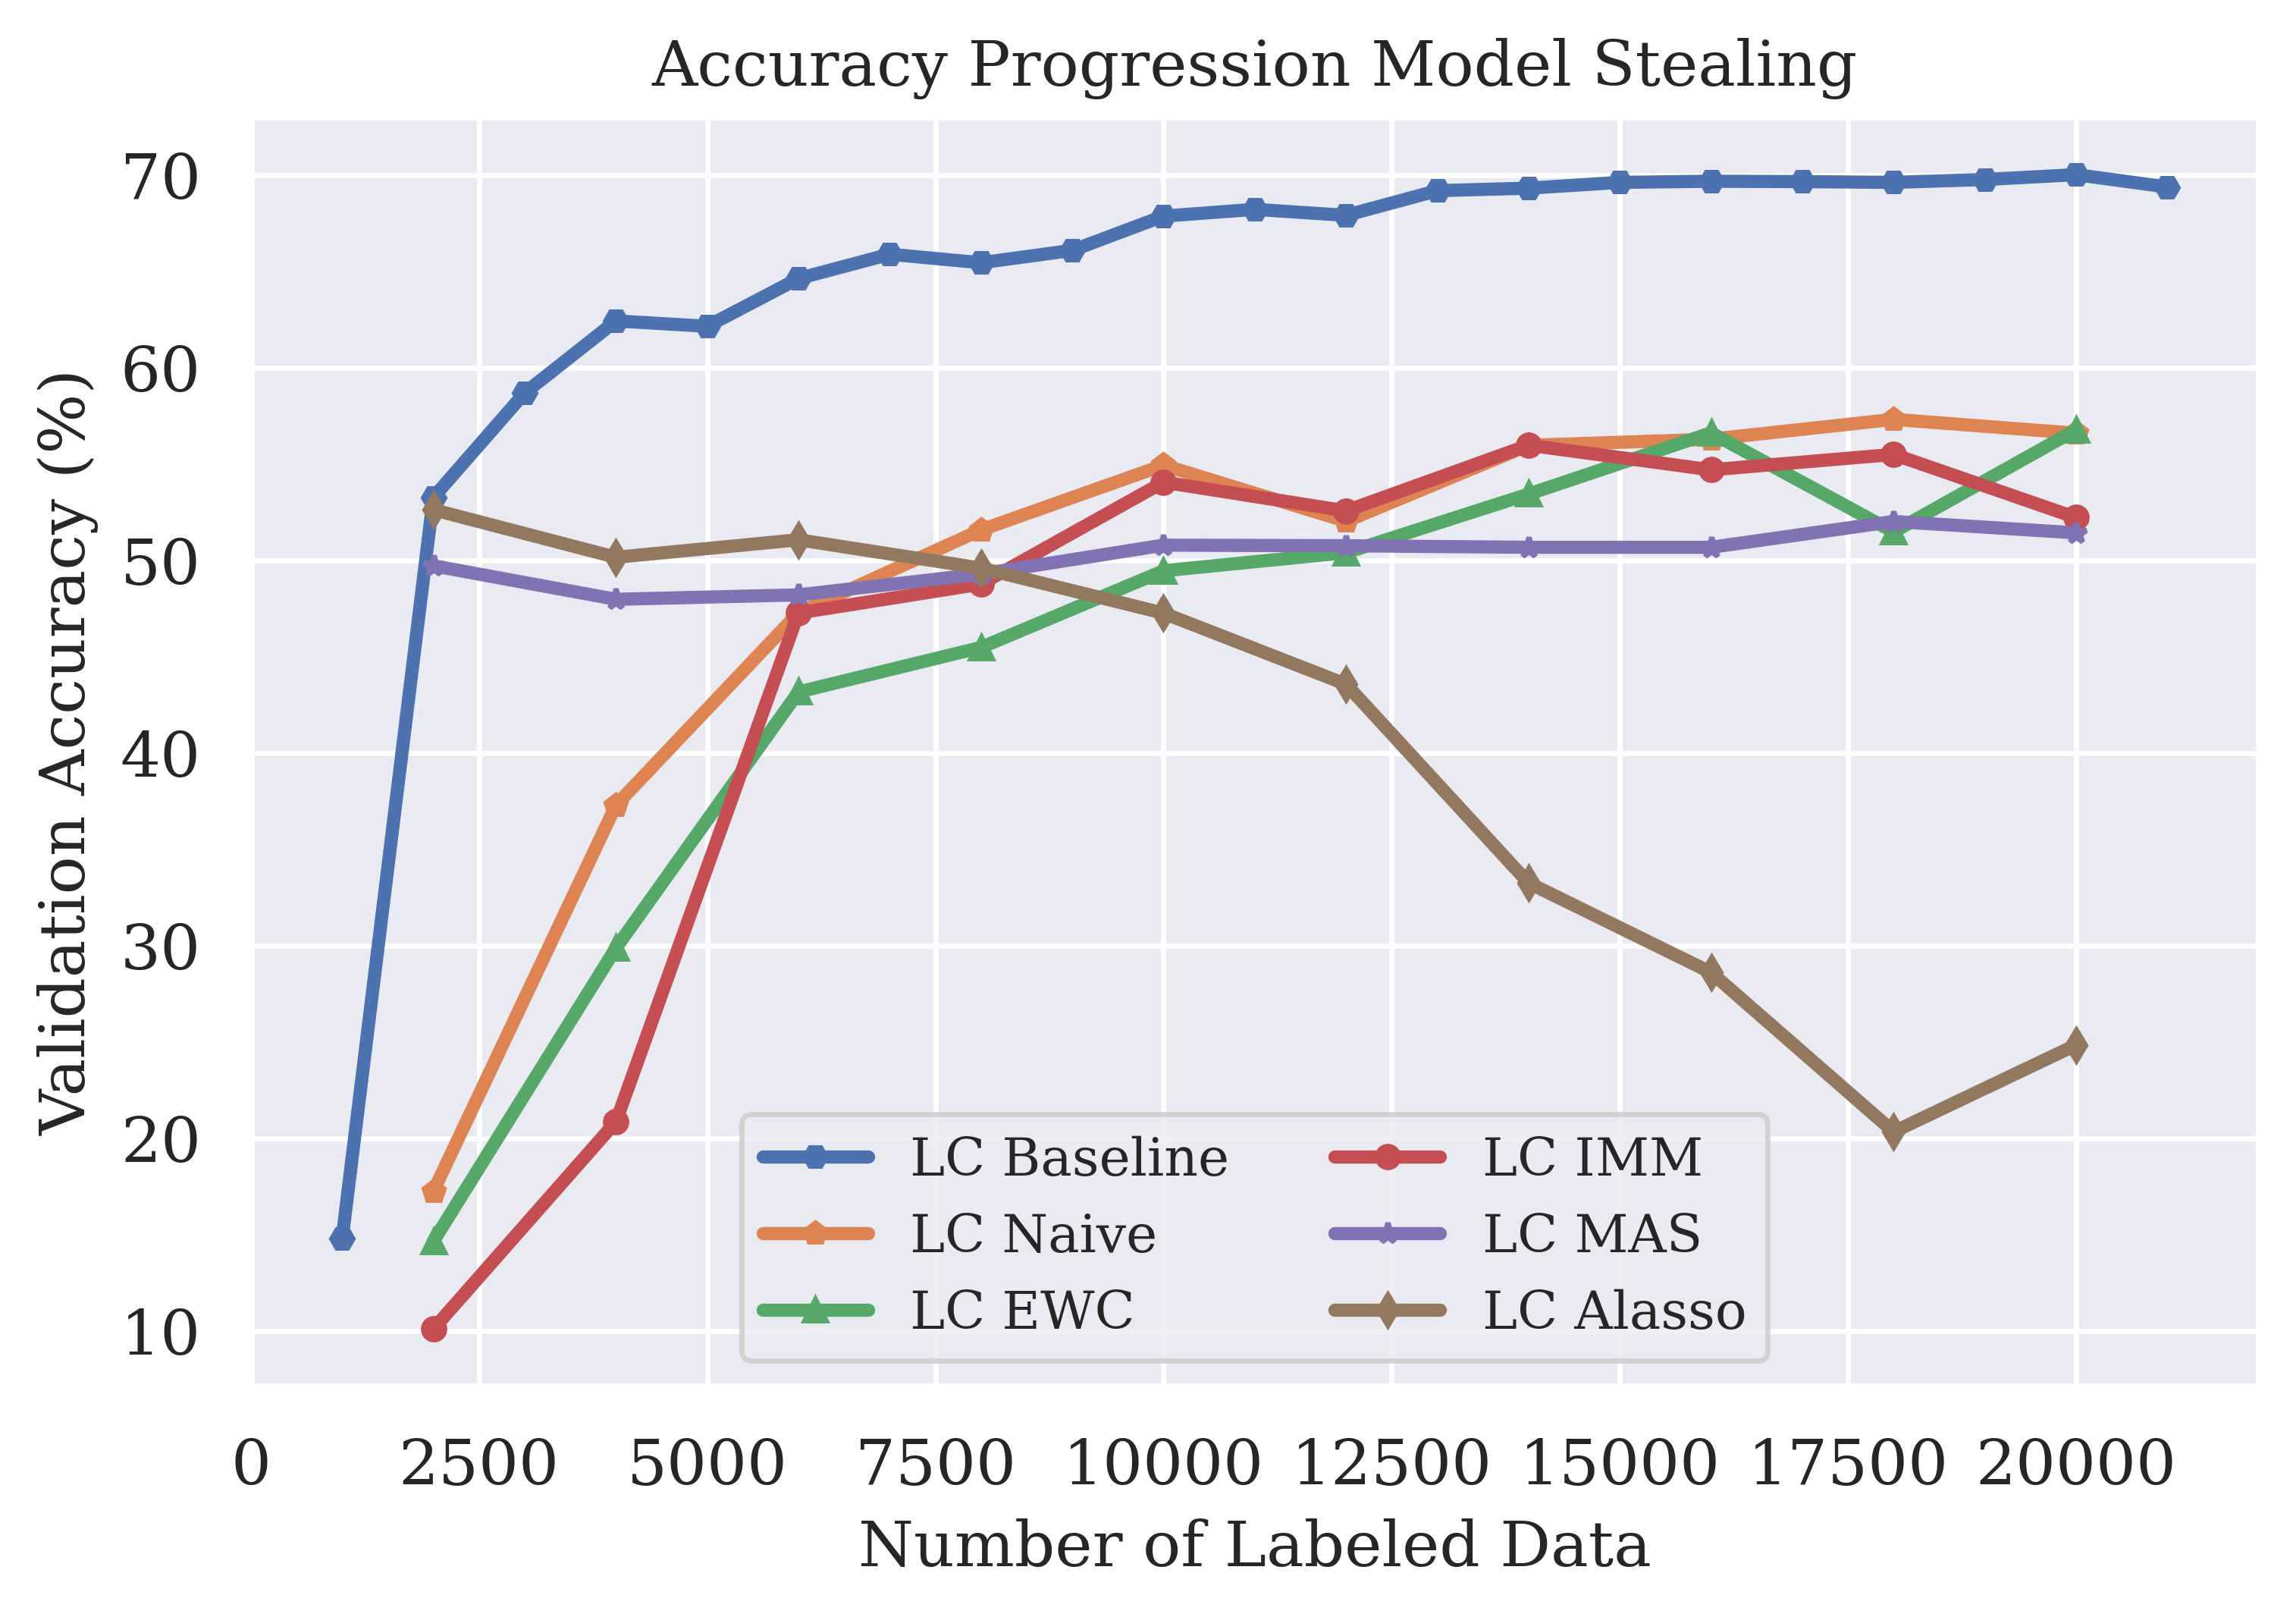
\includegraphics[width=0.48\linewidth]{images/results_CALMS/cifar_softmax_lc.png}
    \caption{Agreement comparison for model stealing on CIFAR-10 using the active learning strategy \gls{lc}.}
    \label{fig:CALMSCIFAR10LC}
\end{figure}

\begin{figure}[!htb]
    \centering
    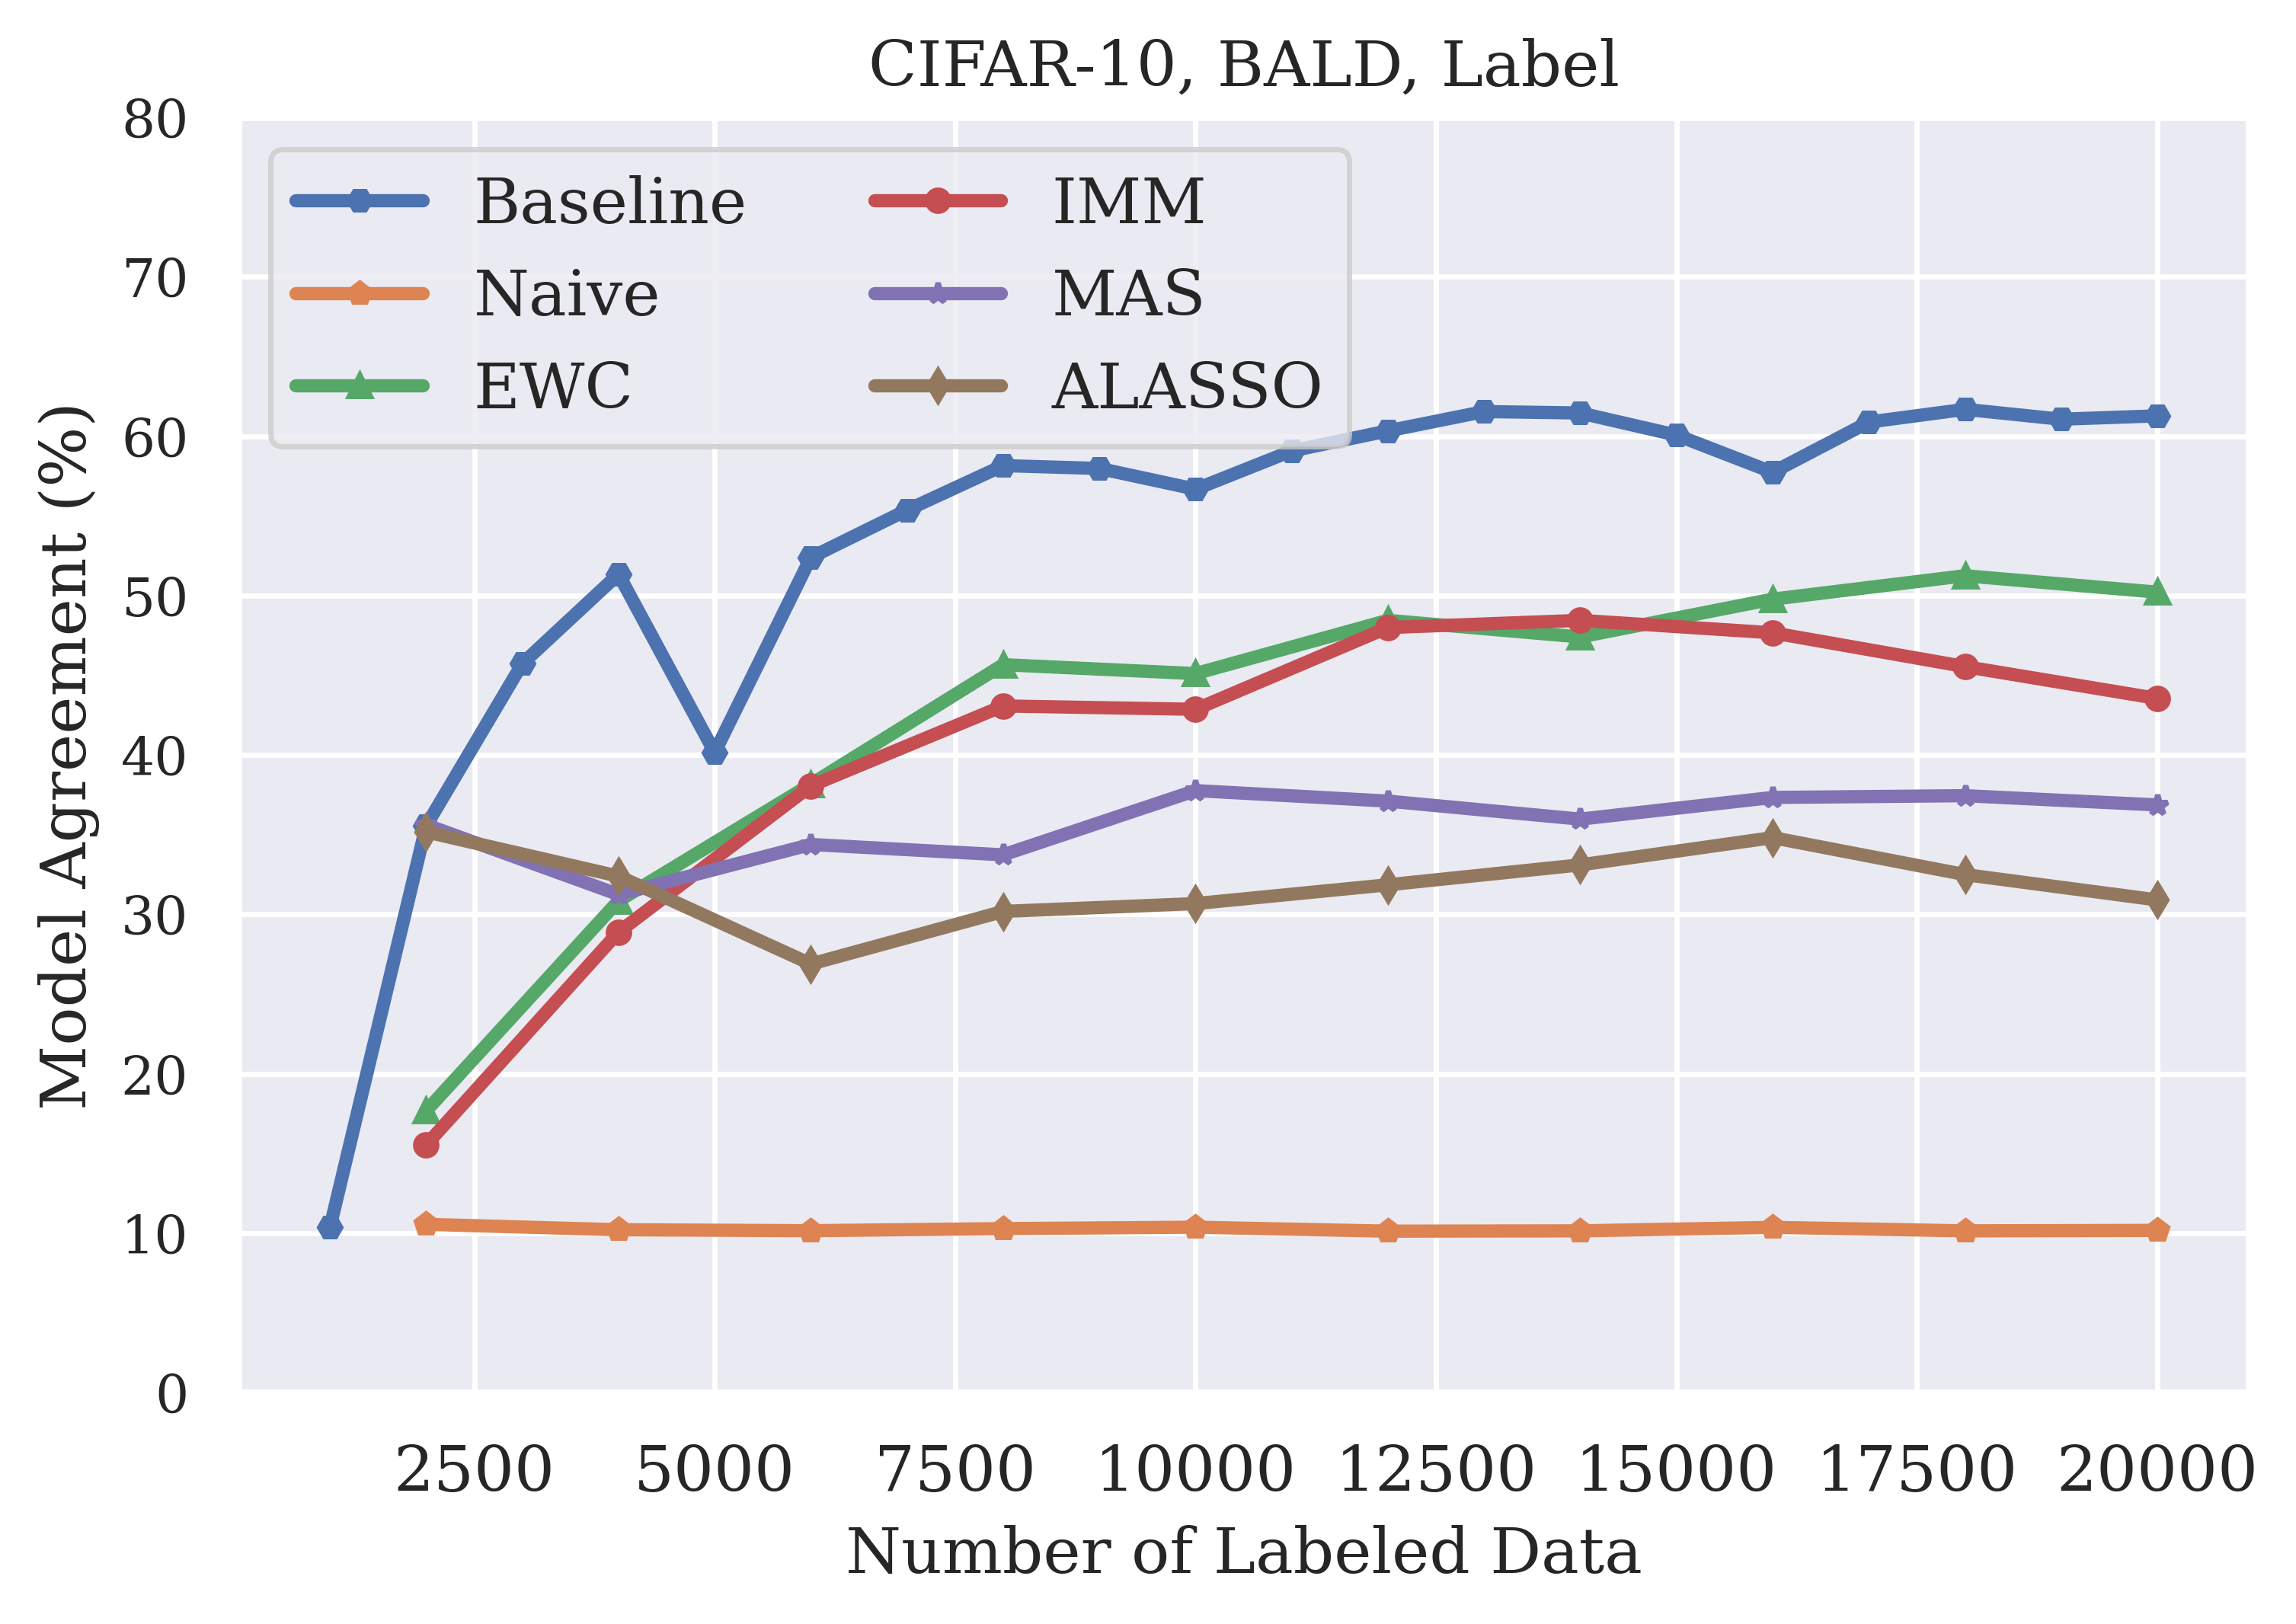
\includegraphics[width=0.48\linewidth]{images/results_CALMS/cifar_label_bald.png} \hfill
    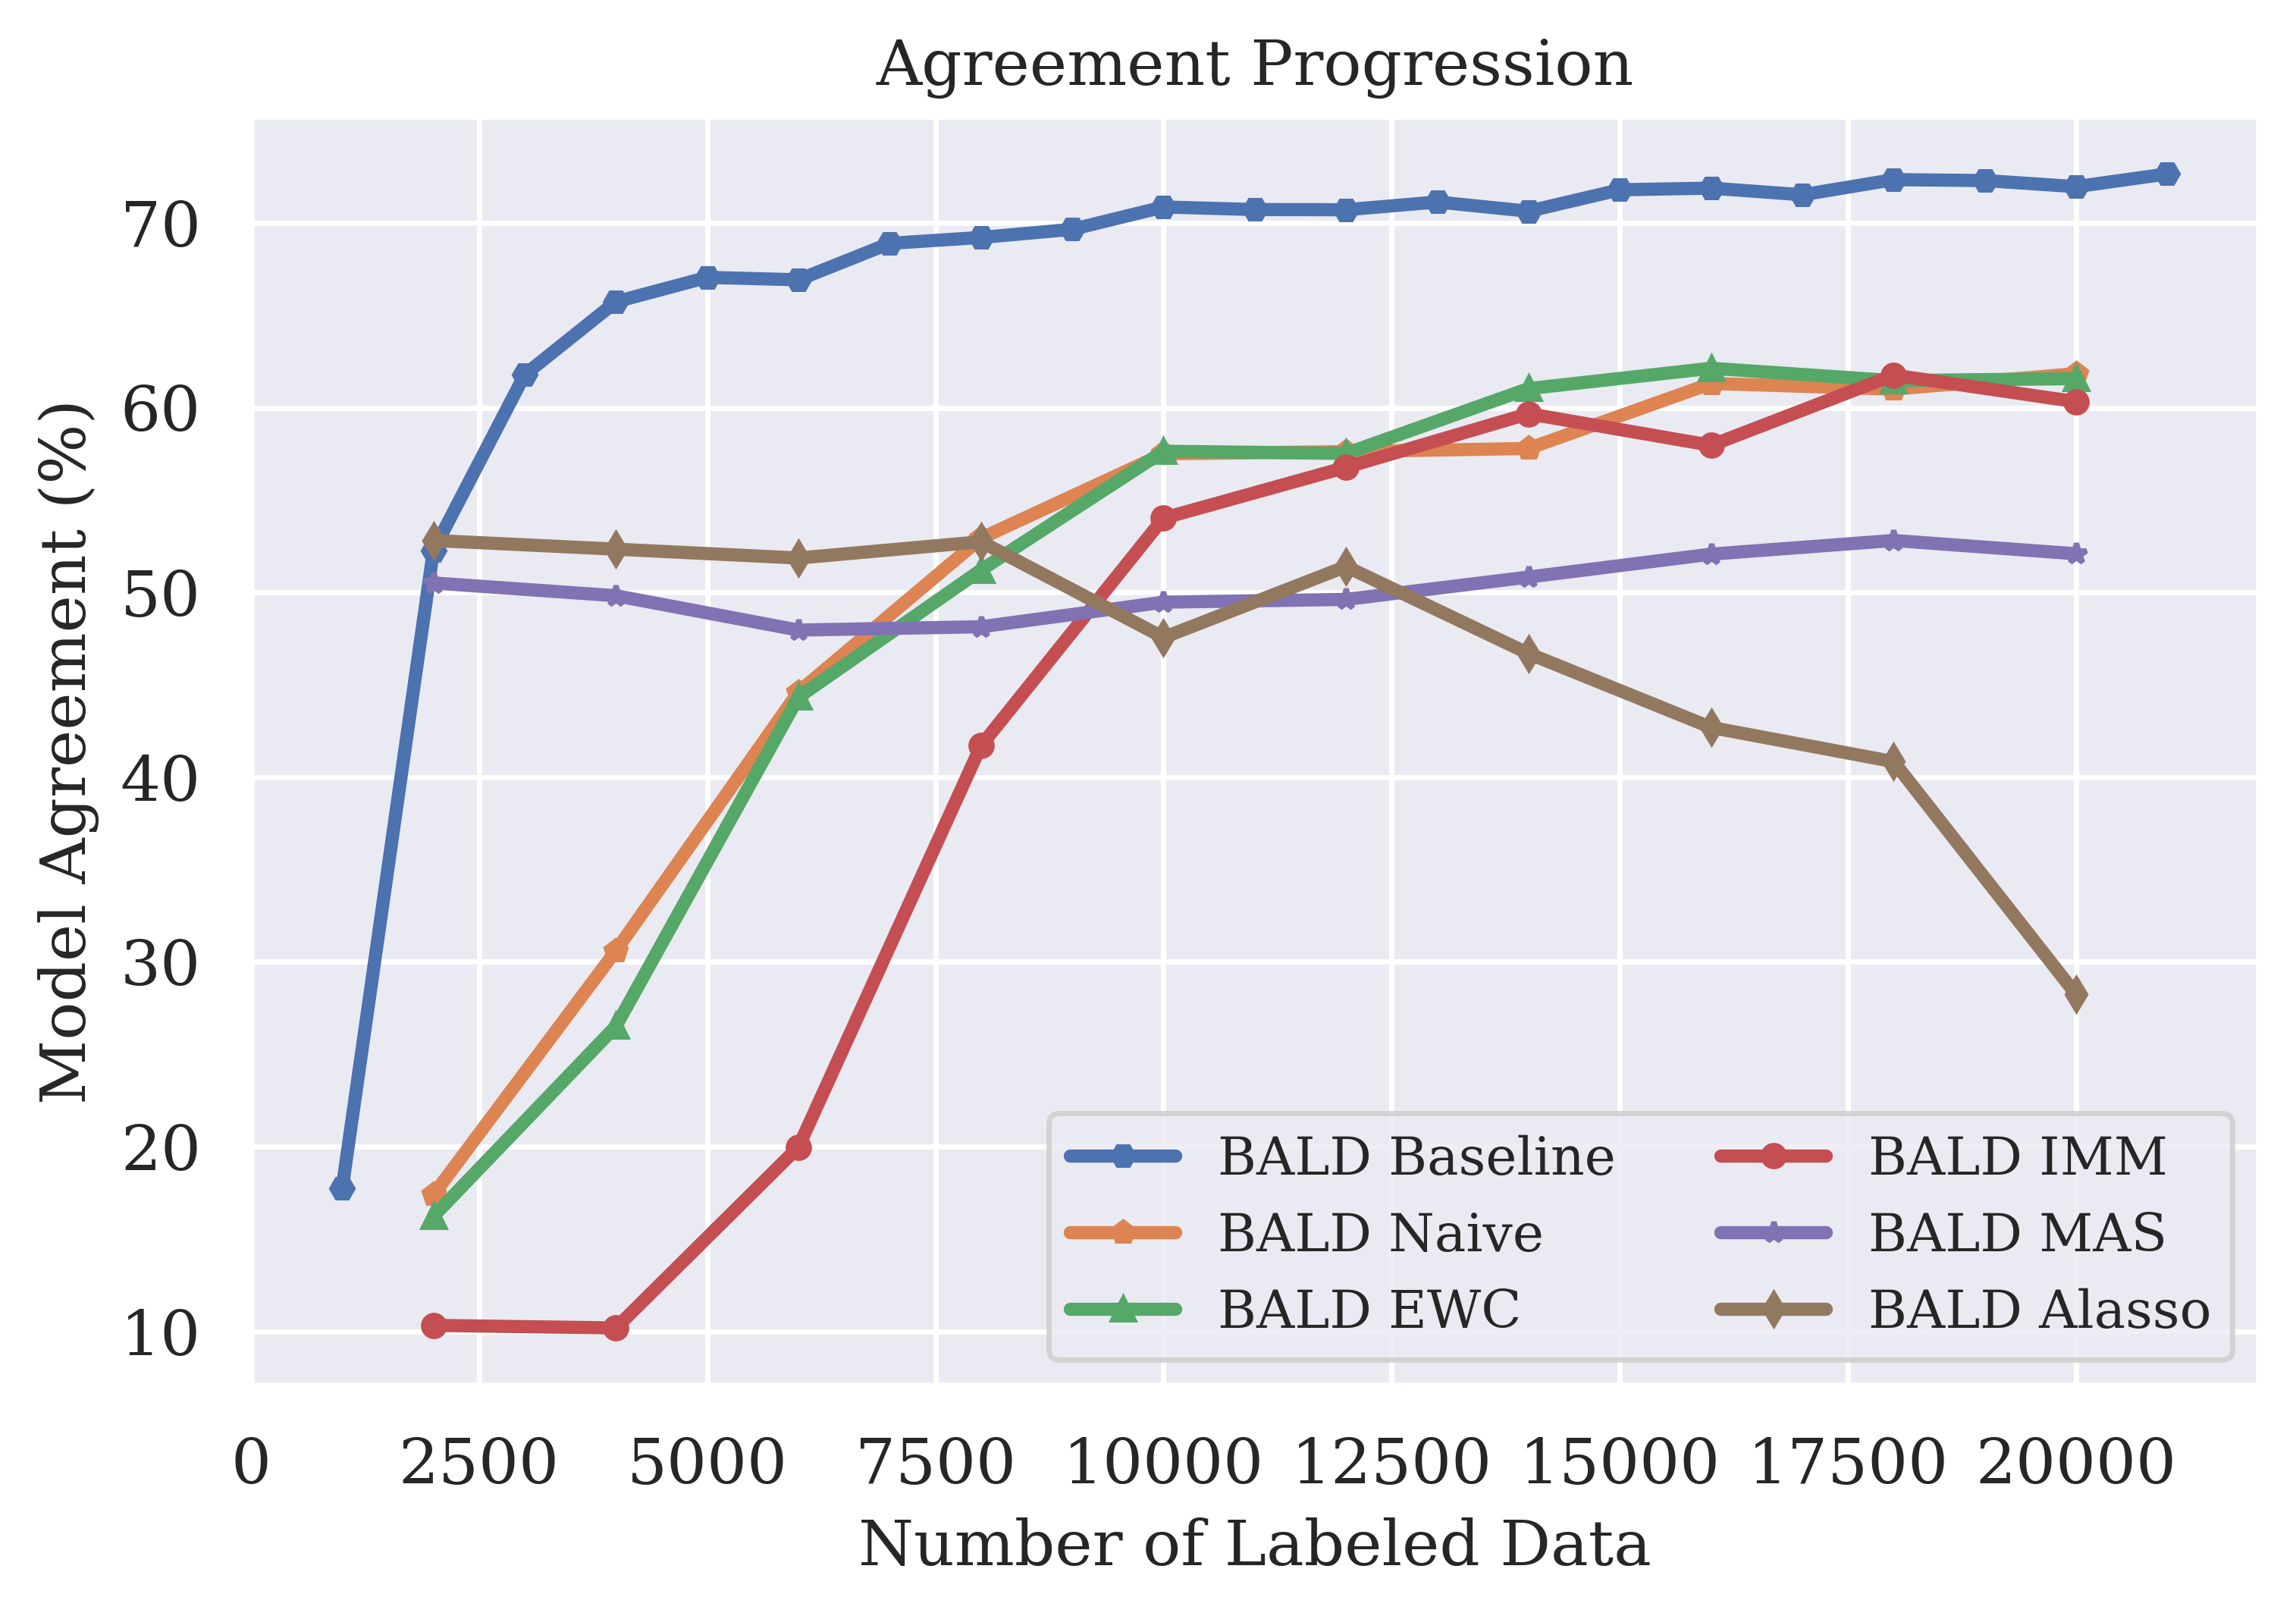
\includegraphics[width=0.48\linewidth]{images/results_CALMS/cifar_softmax_bald.png}
    \caption{Agreement comparison for model stealing on CIFAR-10 using the active learning strategy \gls{bald}.}
    \label{fig:CALMSCIFAR10BALD}
\end{figure}

\begin{figure}[!htb]
    \centering
    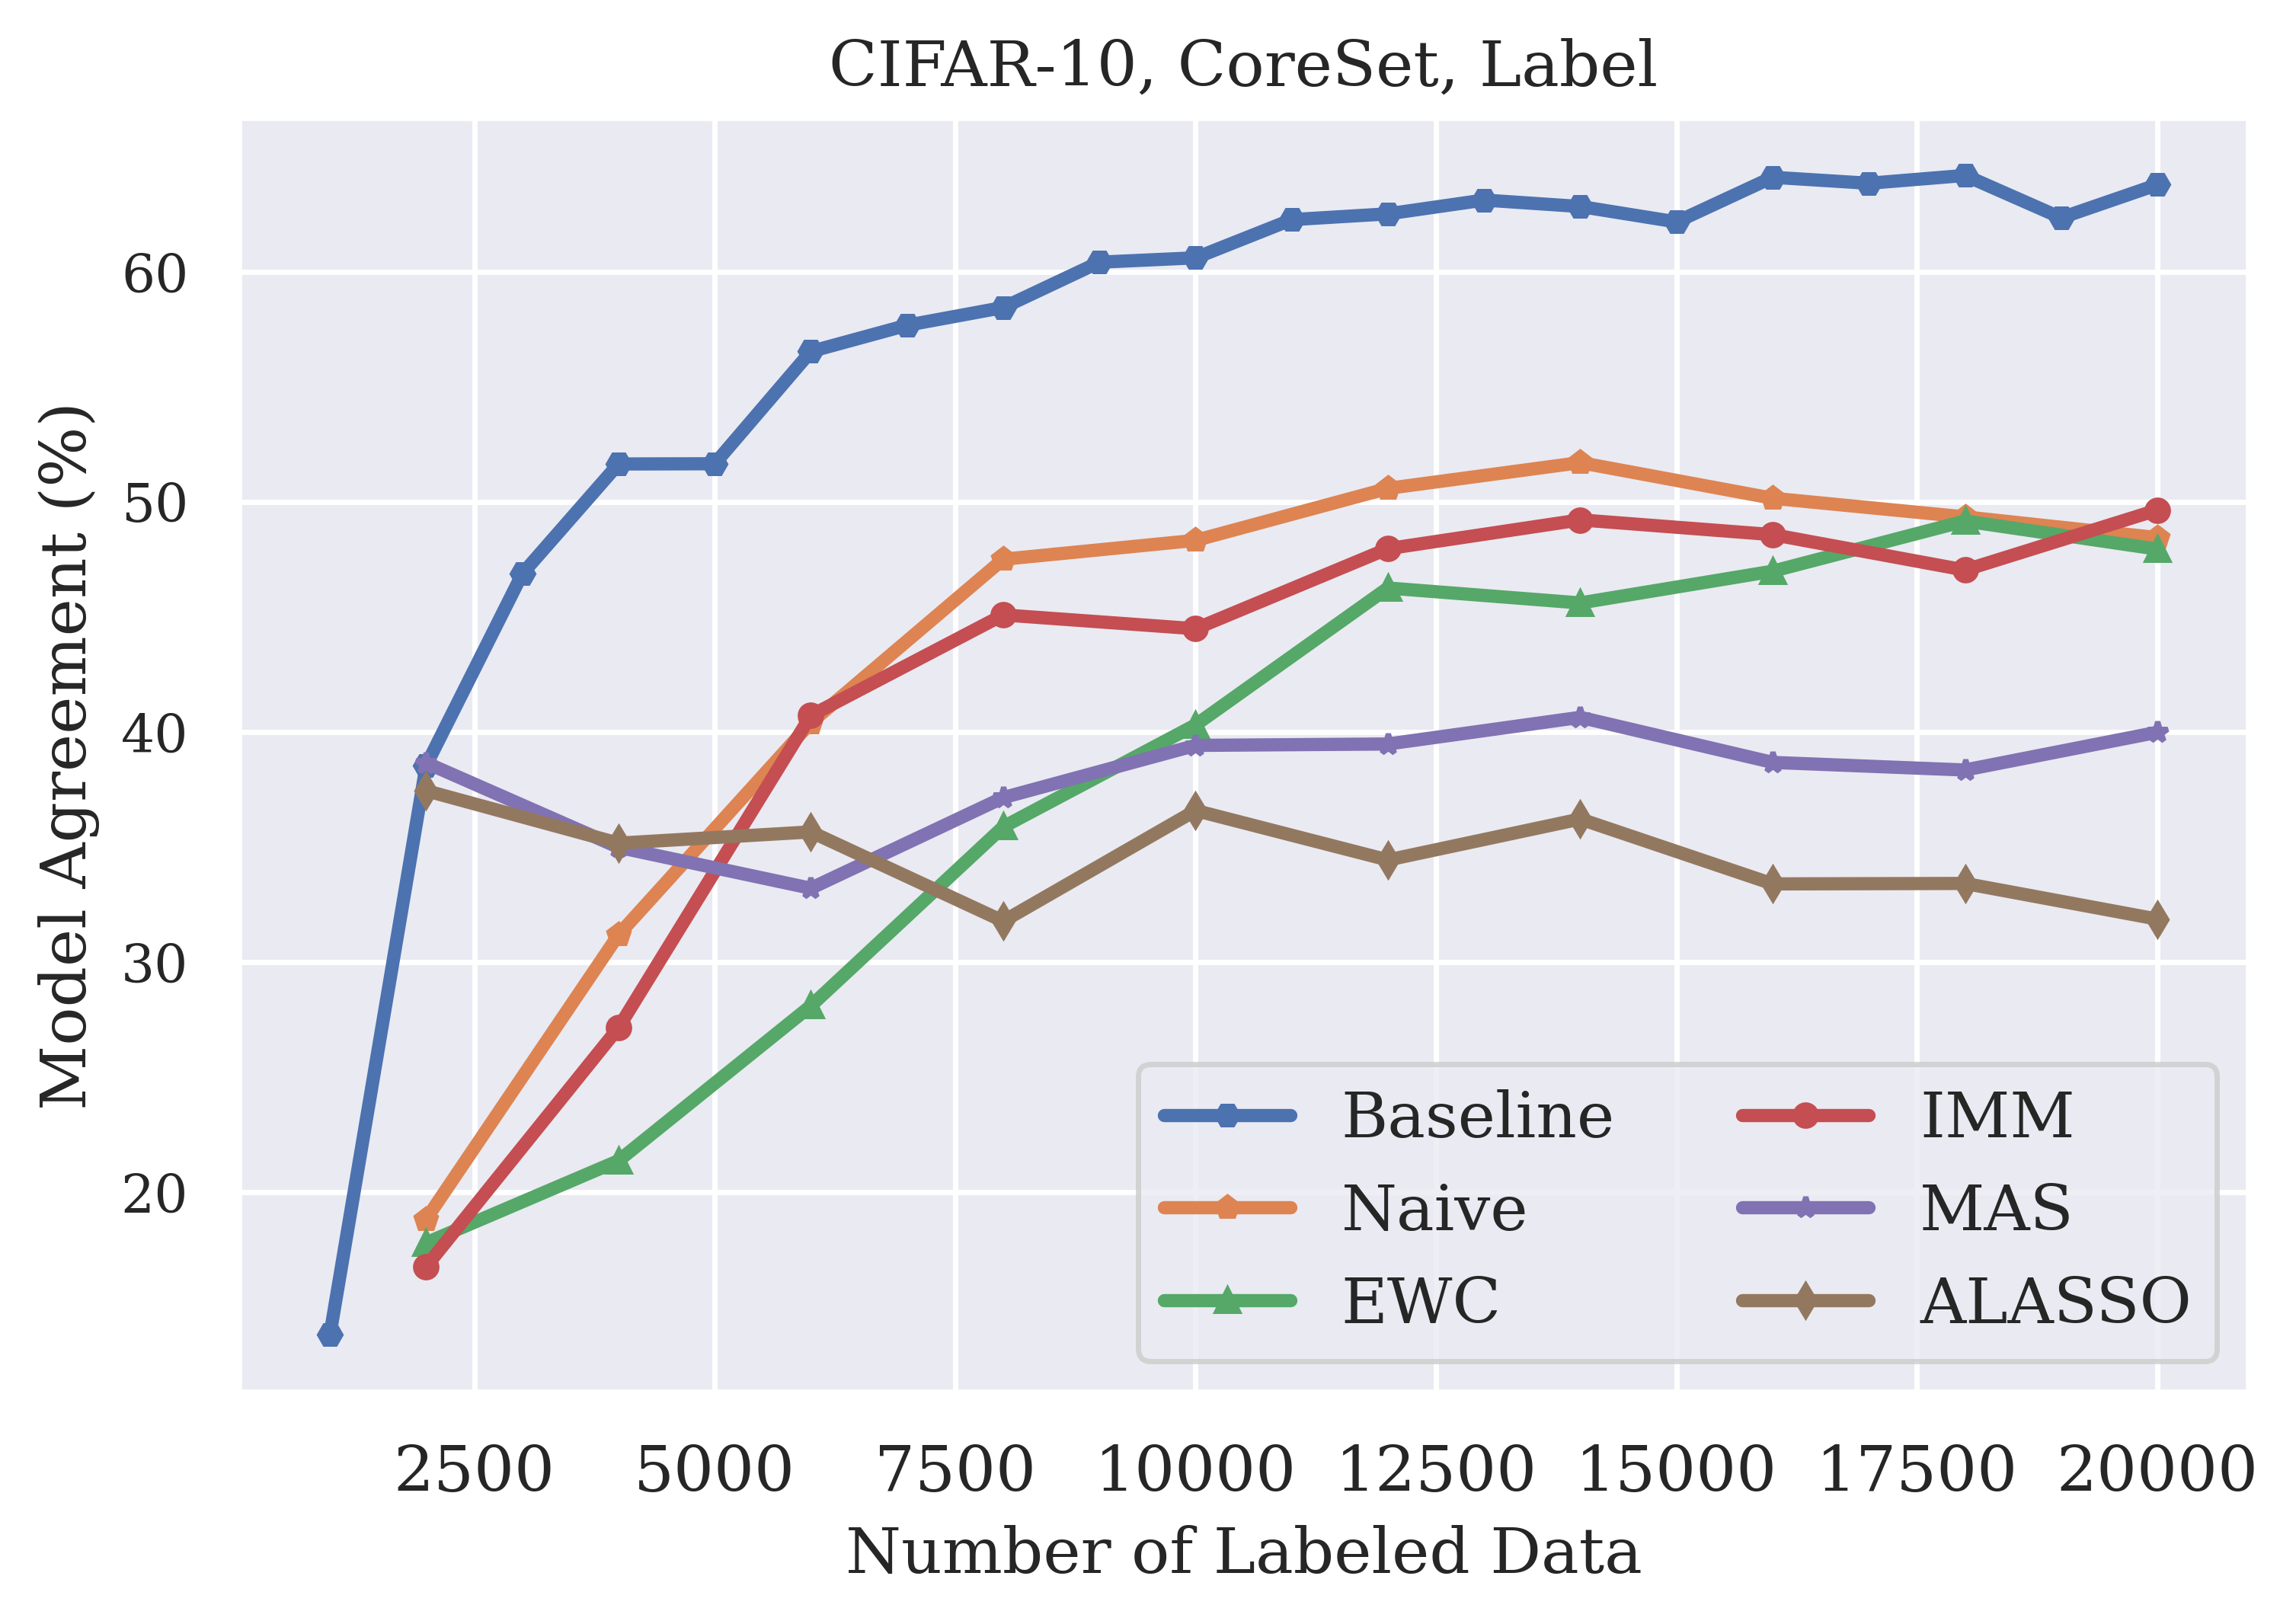
\includegraphics[width=0.48\linewidth]{images/results_CALMS/cifar_label_coreset.png} \hfill
    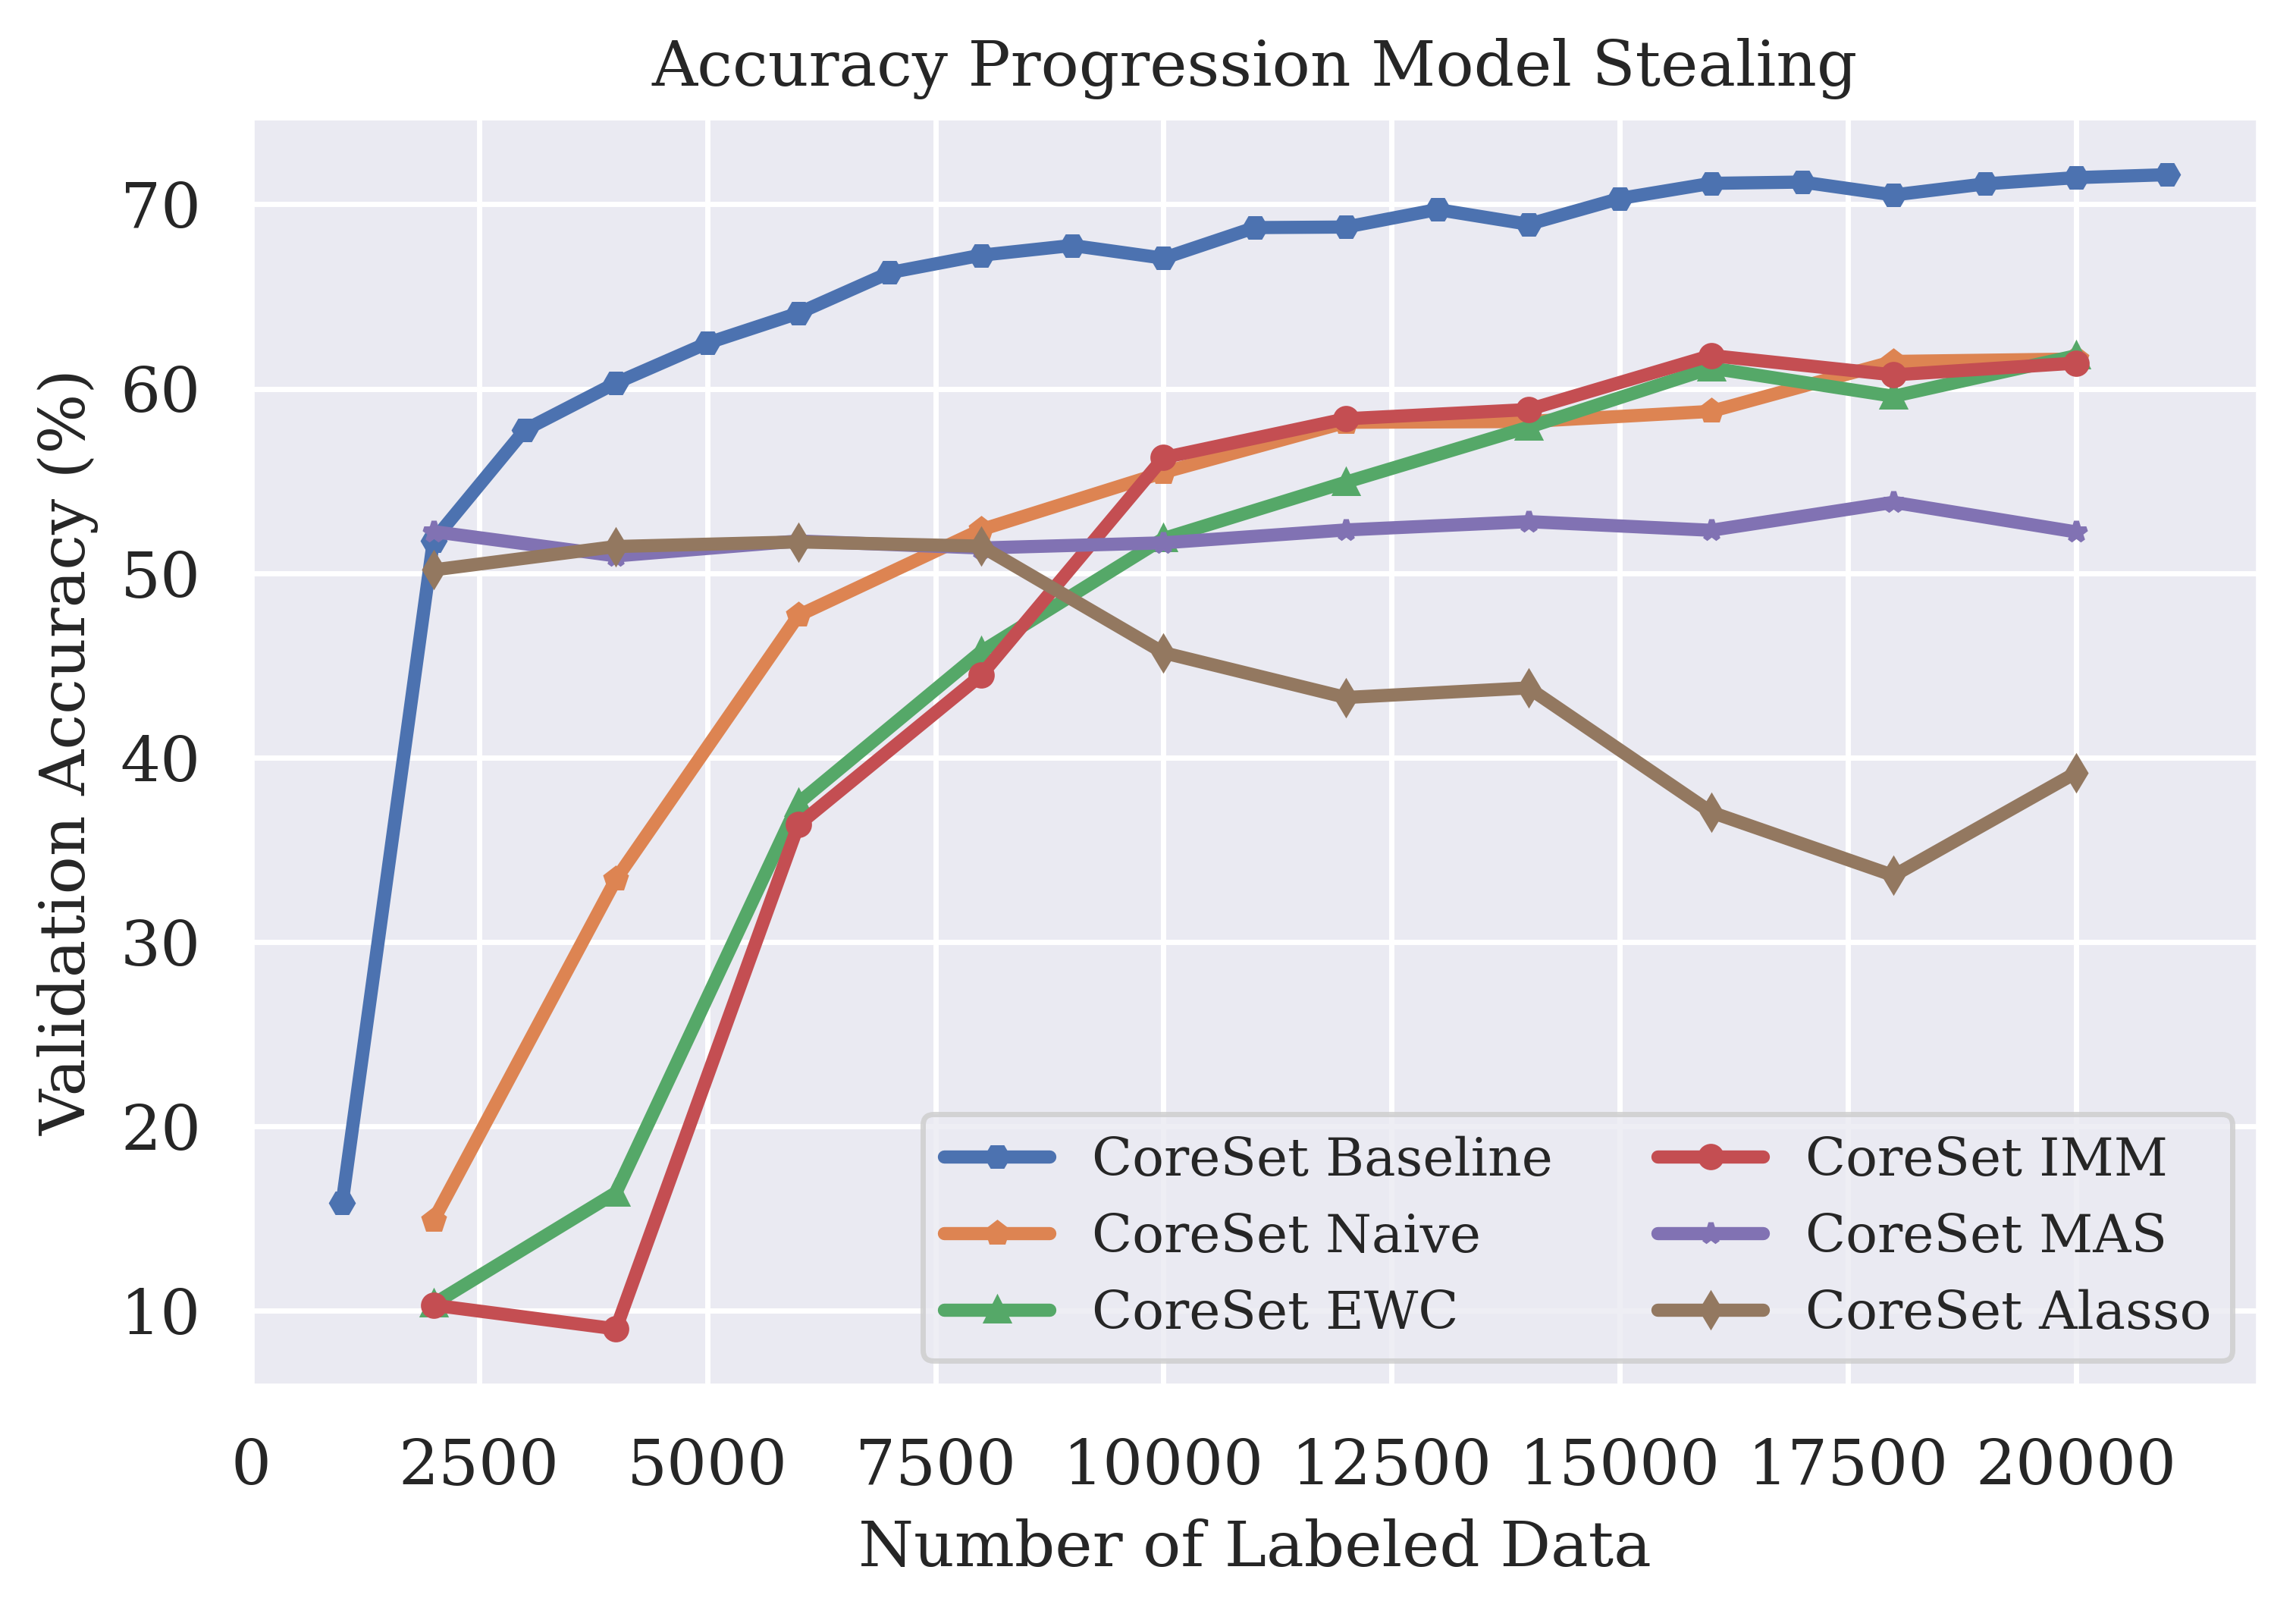
\includegraphics[width=0.48\linewidth]{images/results_CALMS/cifar_softmax_coreset.png}
    \caption{Agreement comparison for model stealing on CIFAR-10 using the active learning strategy CoreSet.}
    \label{fig:CALMSCIFAR10CoreSet}
\end{figure}

\begin{figure}[!htb]
    \centering
    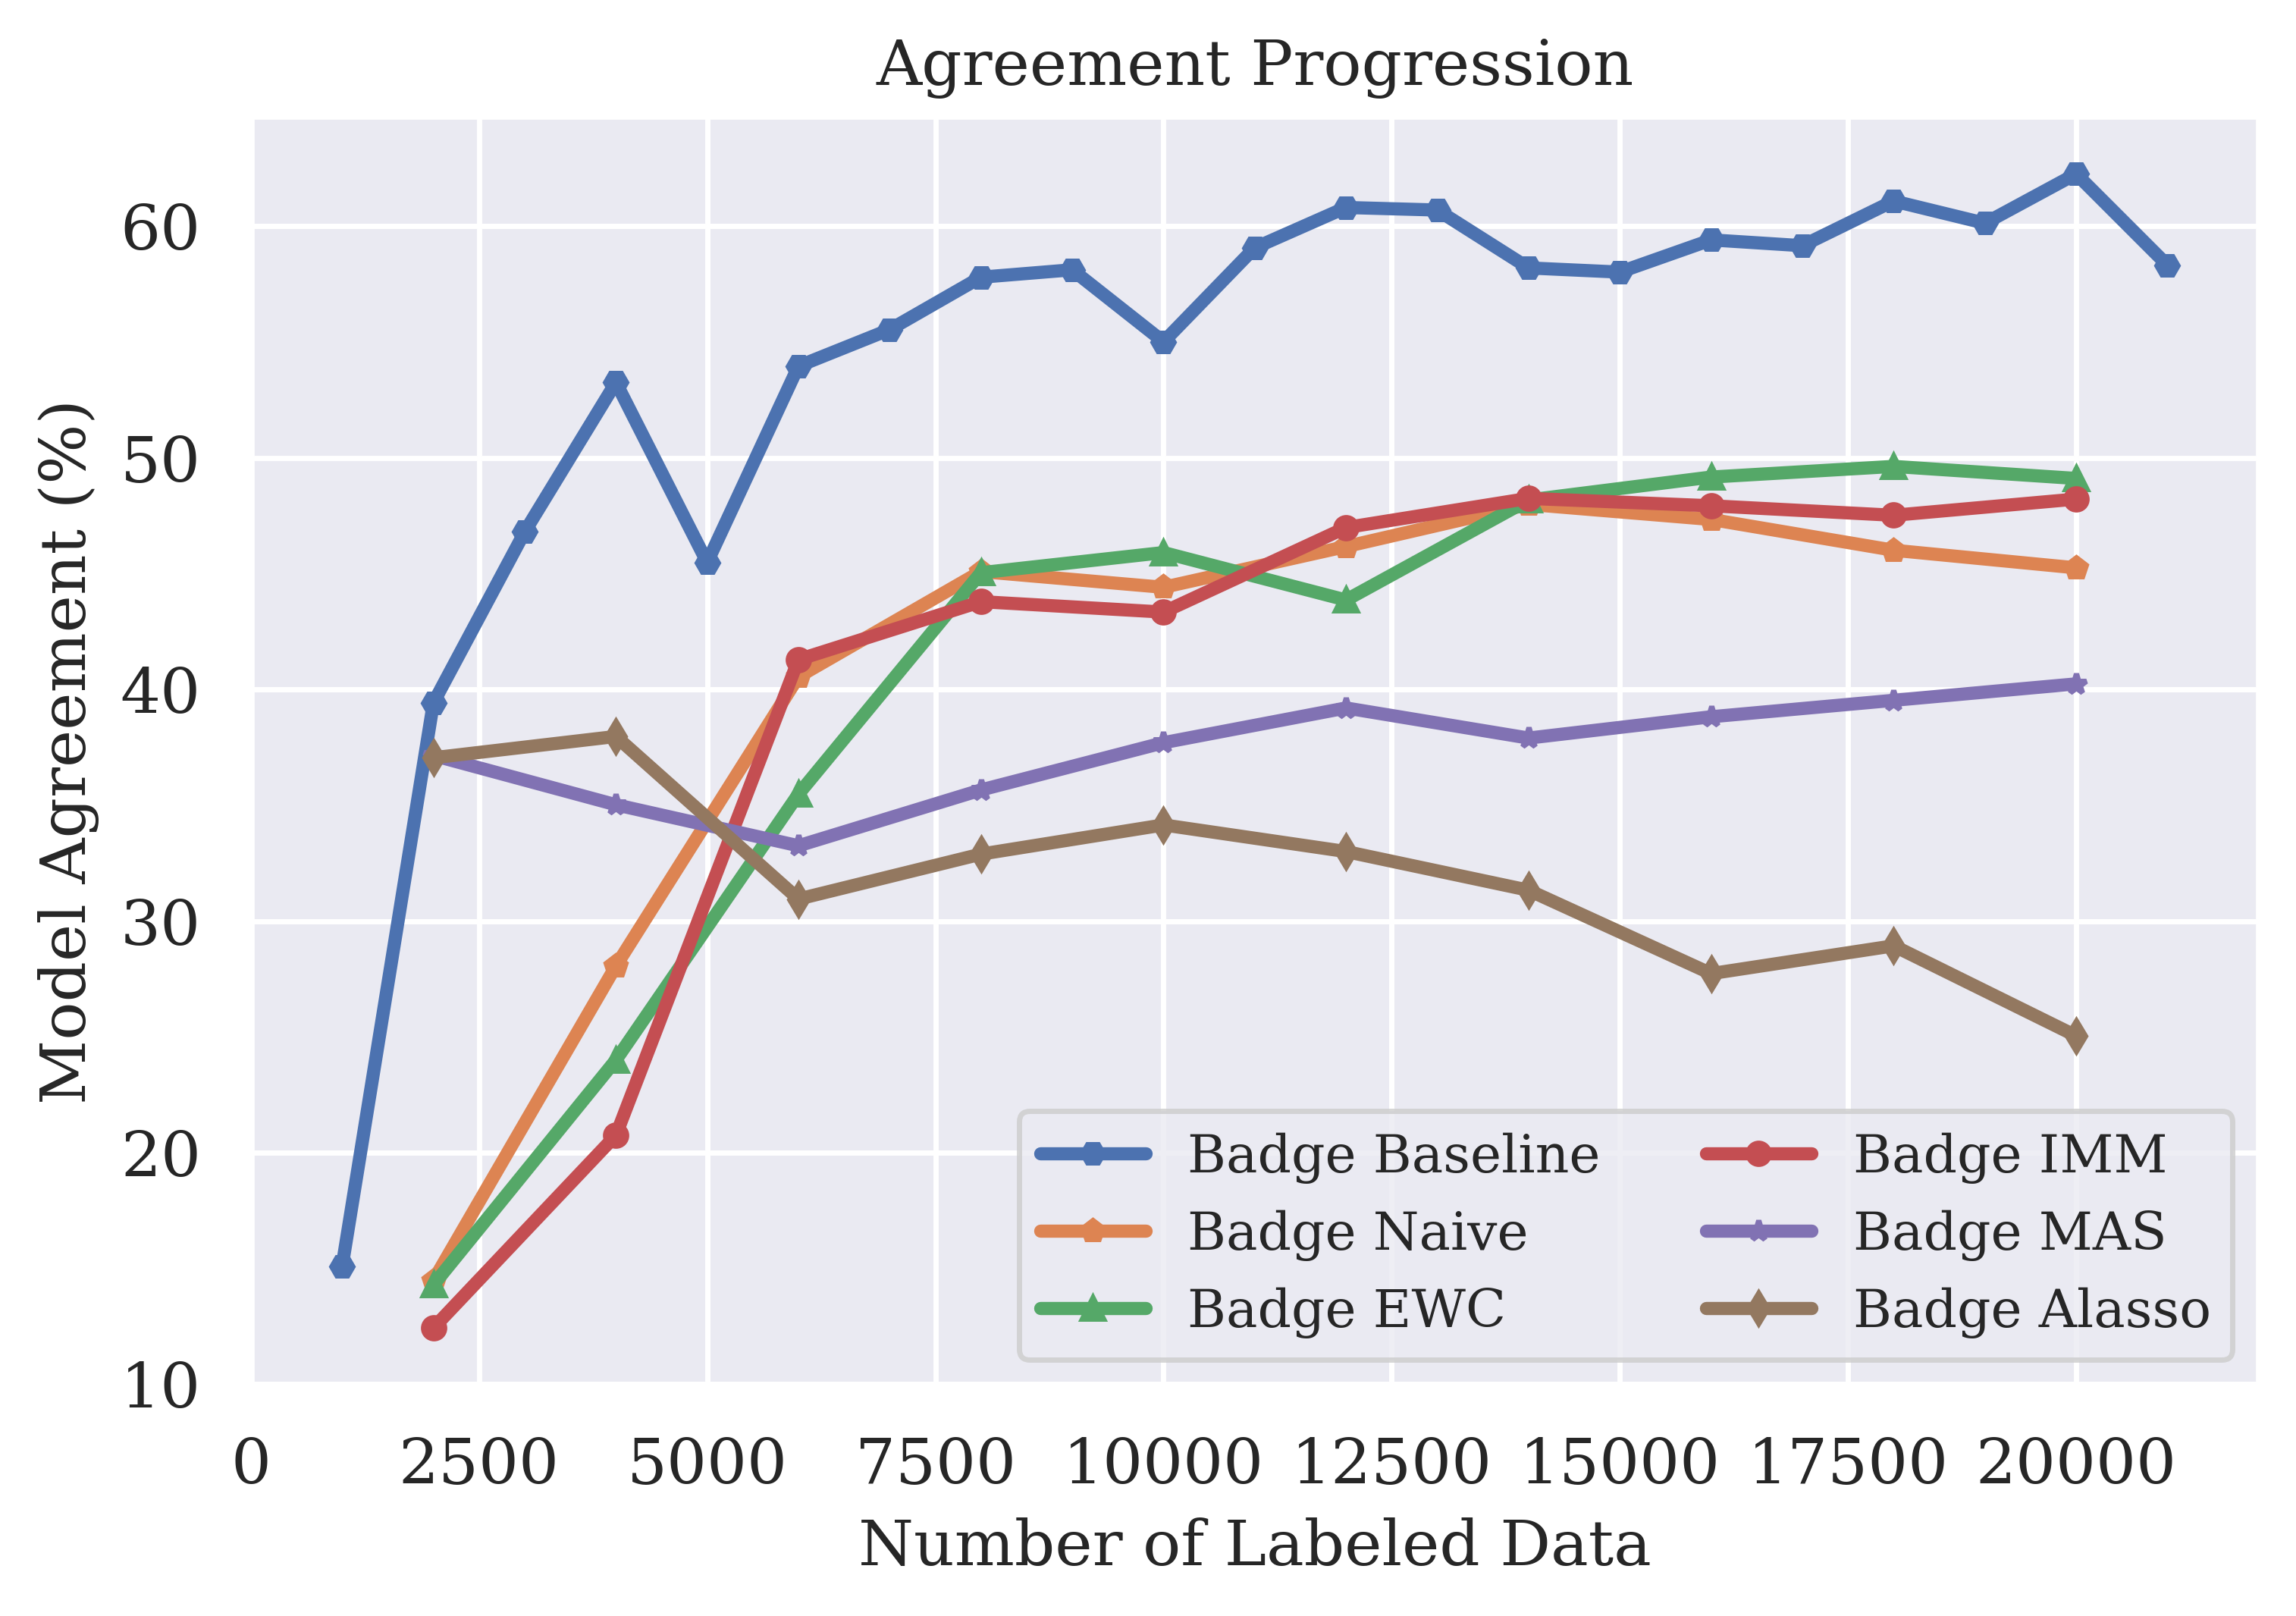
\includegraphics[width=0.48\linewidth]{images/results_CALMS/cifar_label_badge.png} \hfill
    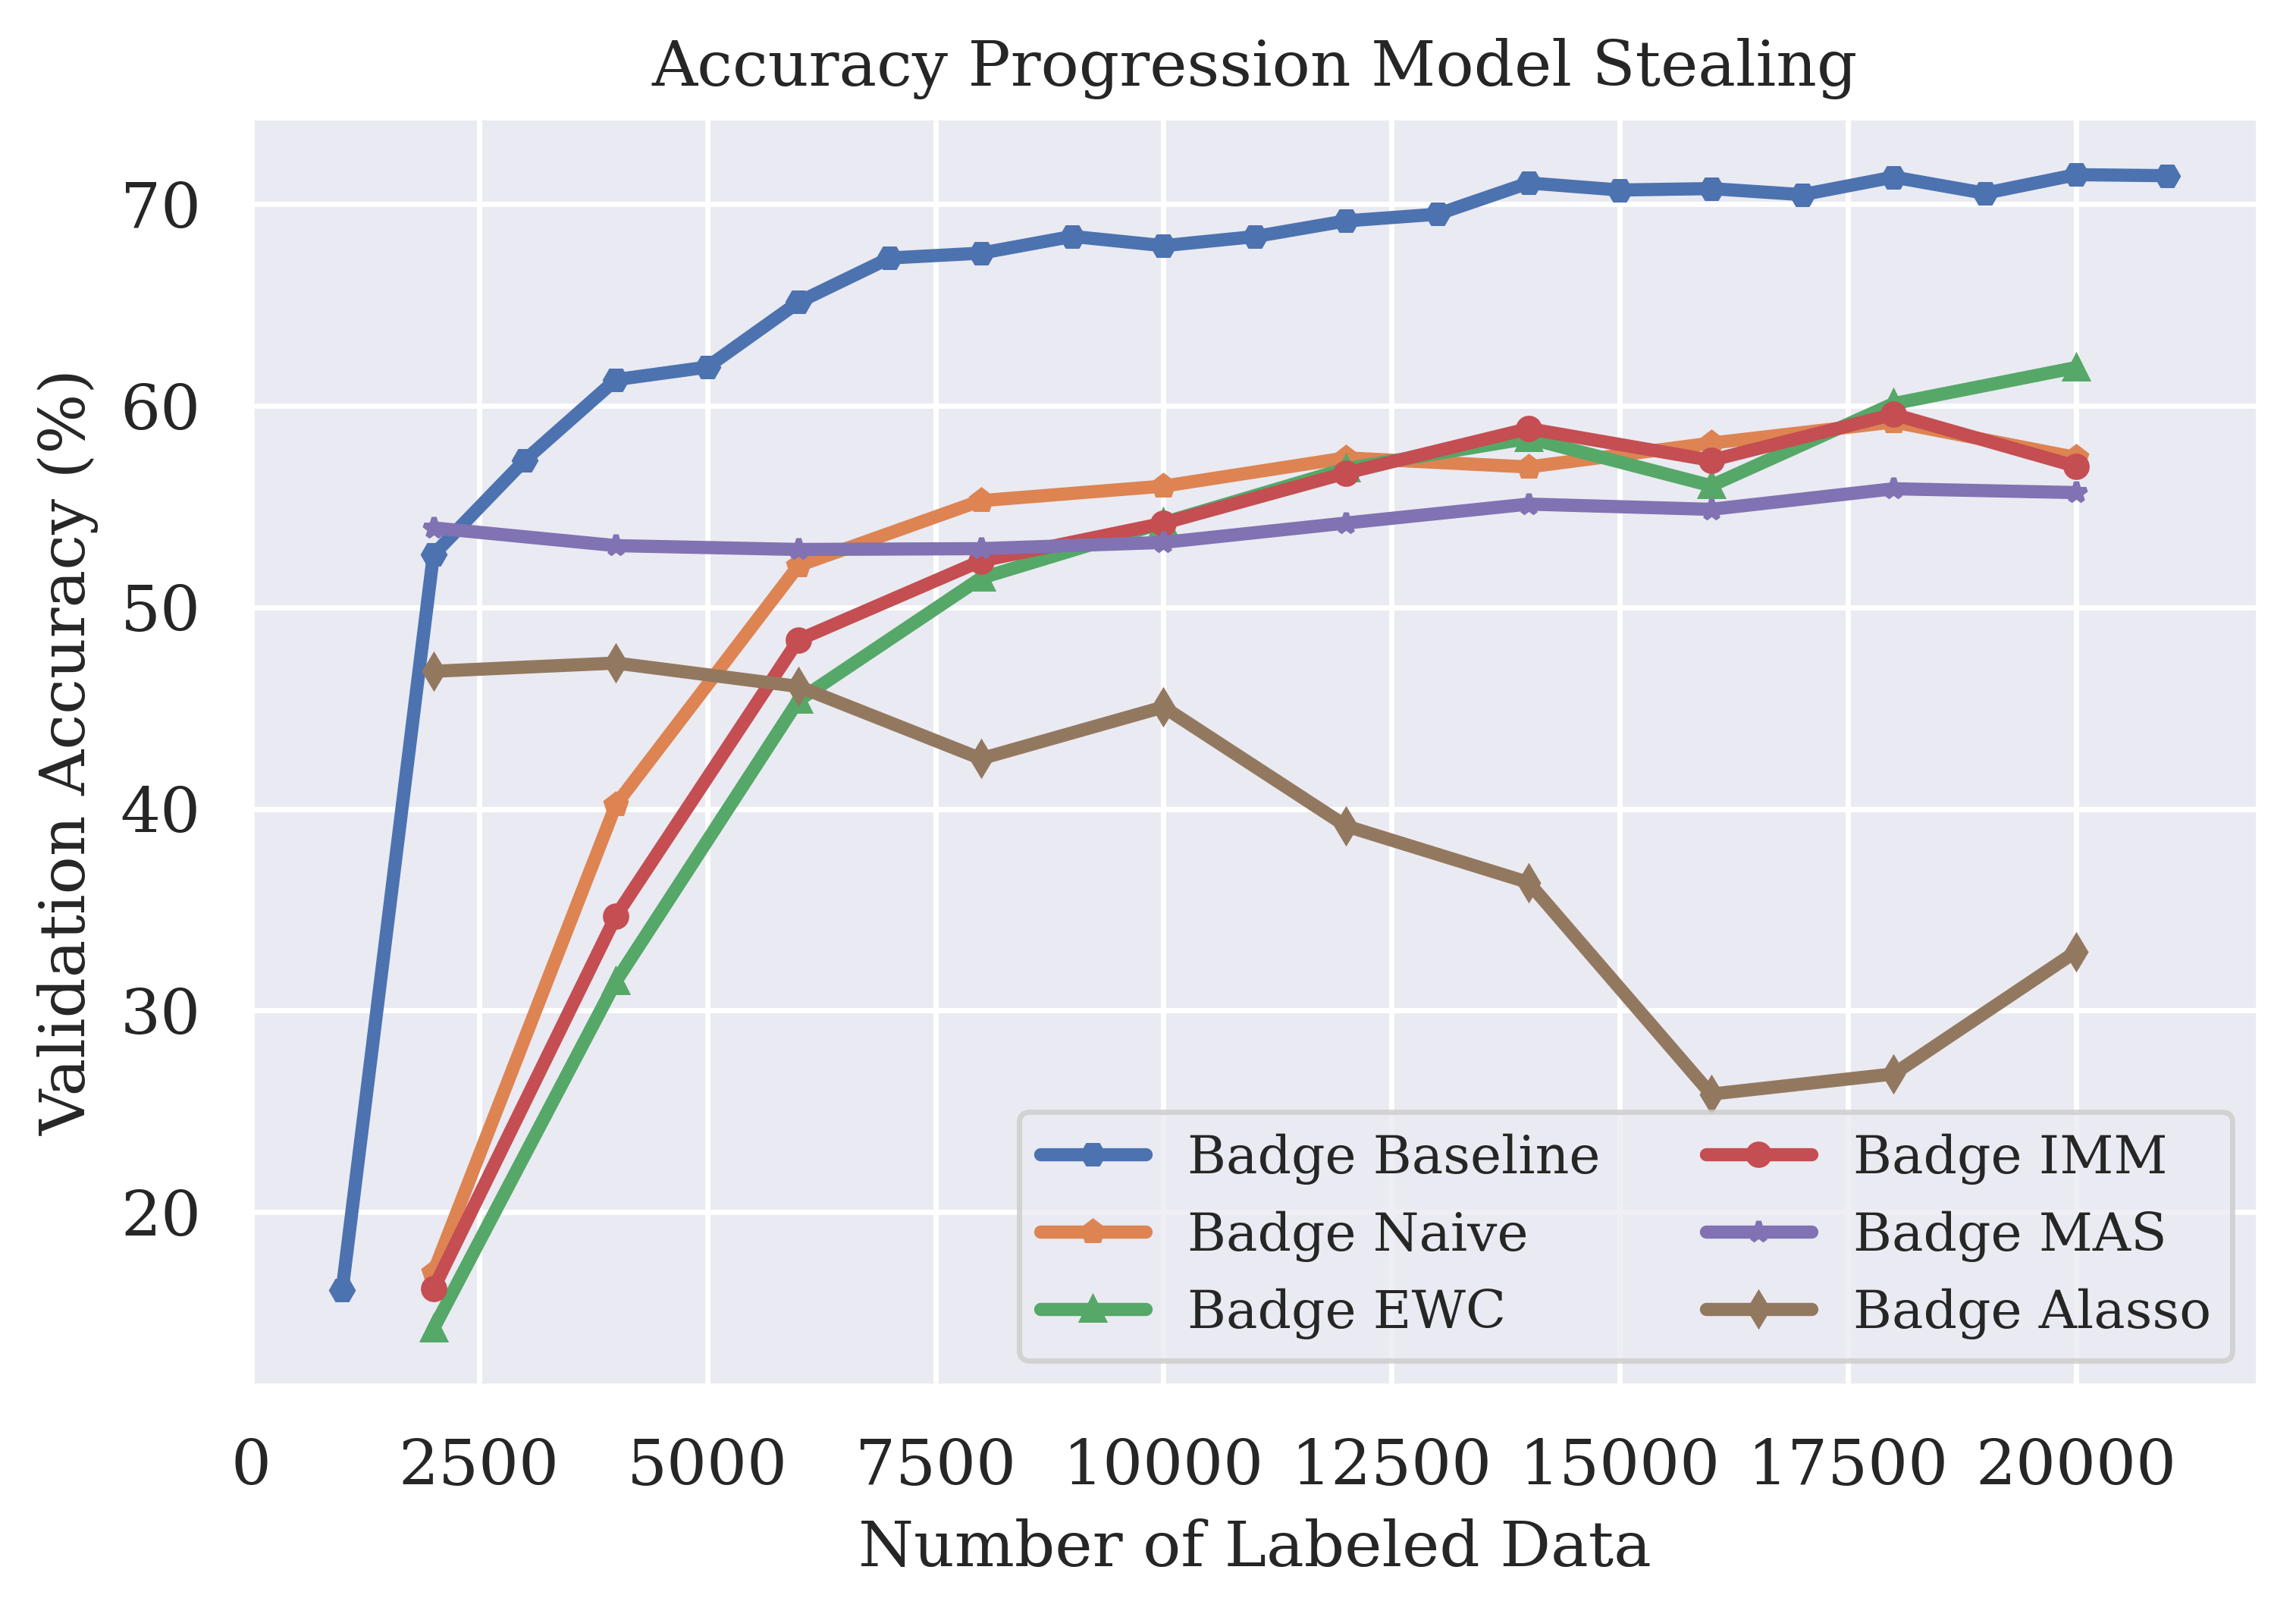
\includegraphics[width=0.48\linewidth]{images/results_CALMS/cifar_softmax_badge.png}
    \caption{Agreement comparison for model stealing on CIFAR-10 using the active learning strategy \gls{badge}.}
    \label{fig:CALMSCIFAR10Badge}
\end{figure}

\clearpage

\subsubsection{CIFAR-100}
\label{sec:Appendix:CALMS:CIFAR100}
In this section, we present the complete runs of all experiments which involve continual active learning using CIFAR-100 as a target model dataset.

\begin{figure}[!htb]
    \centering
    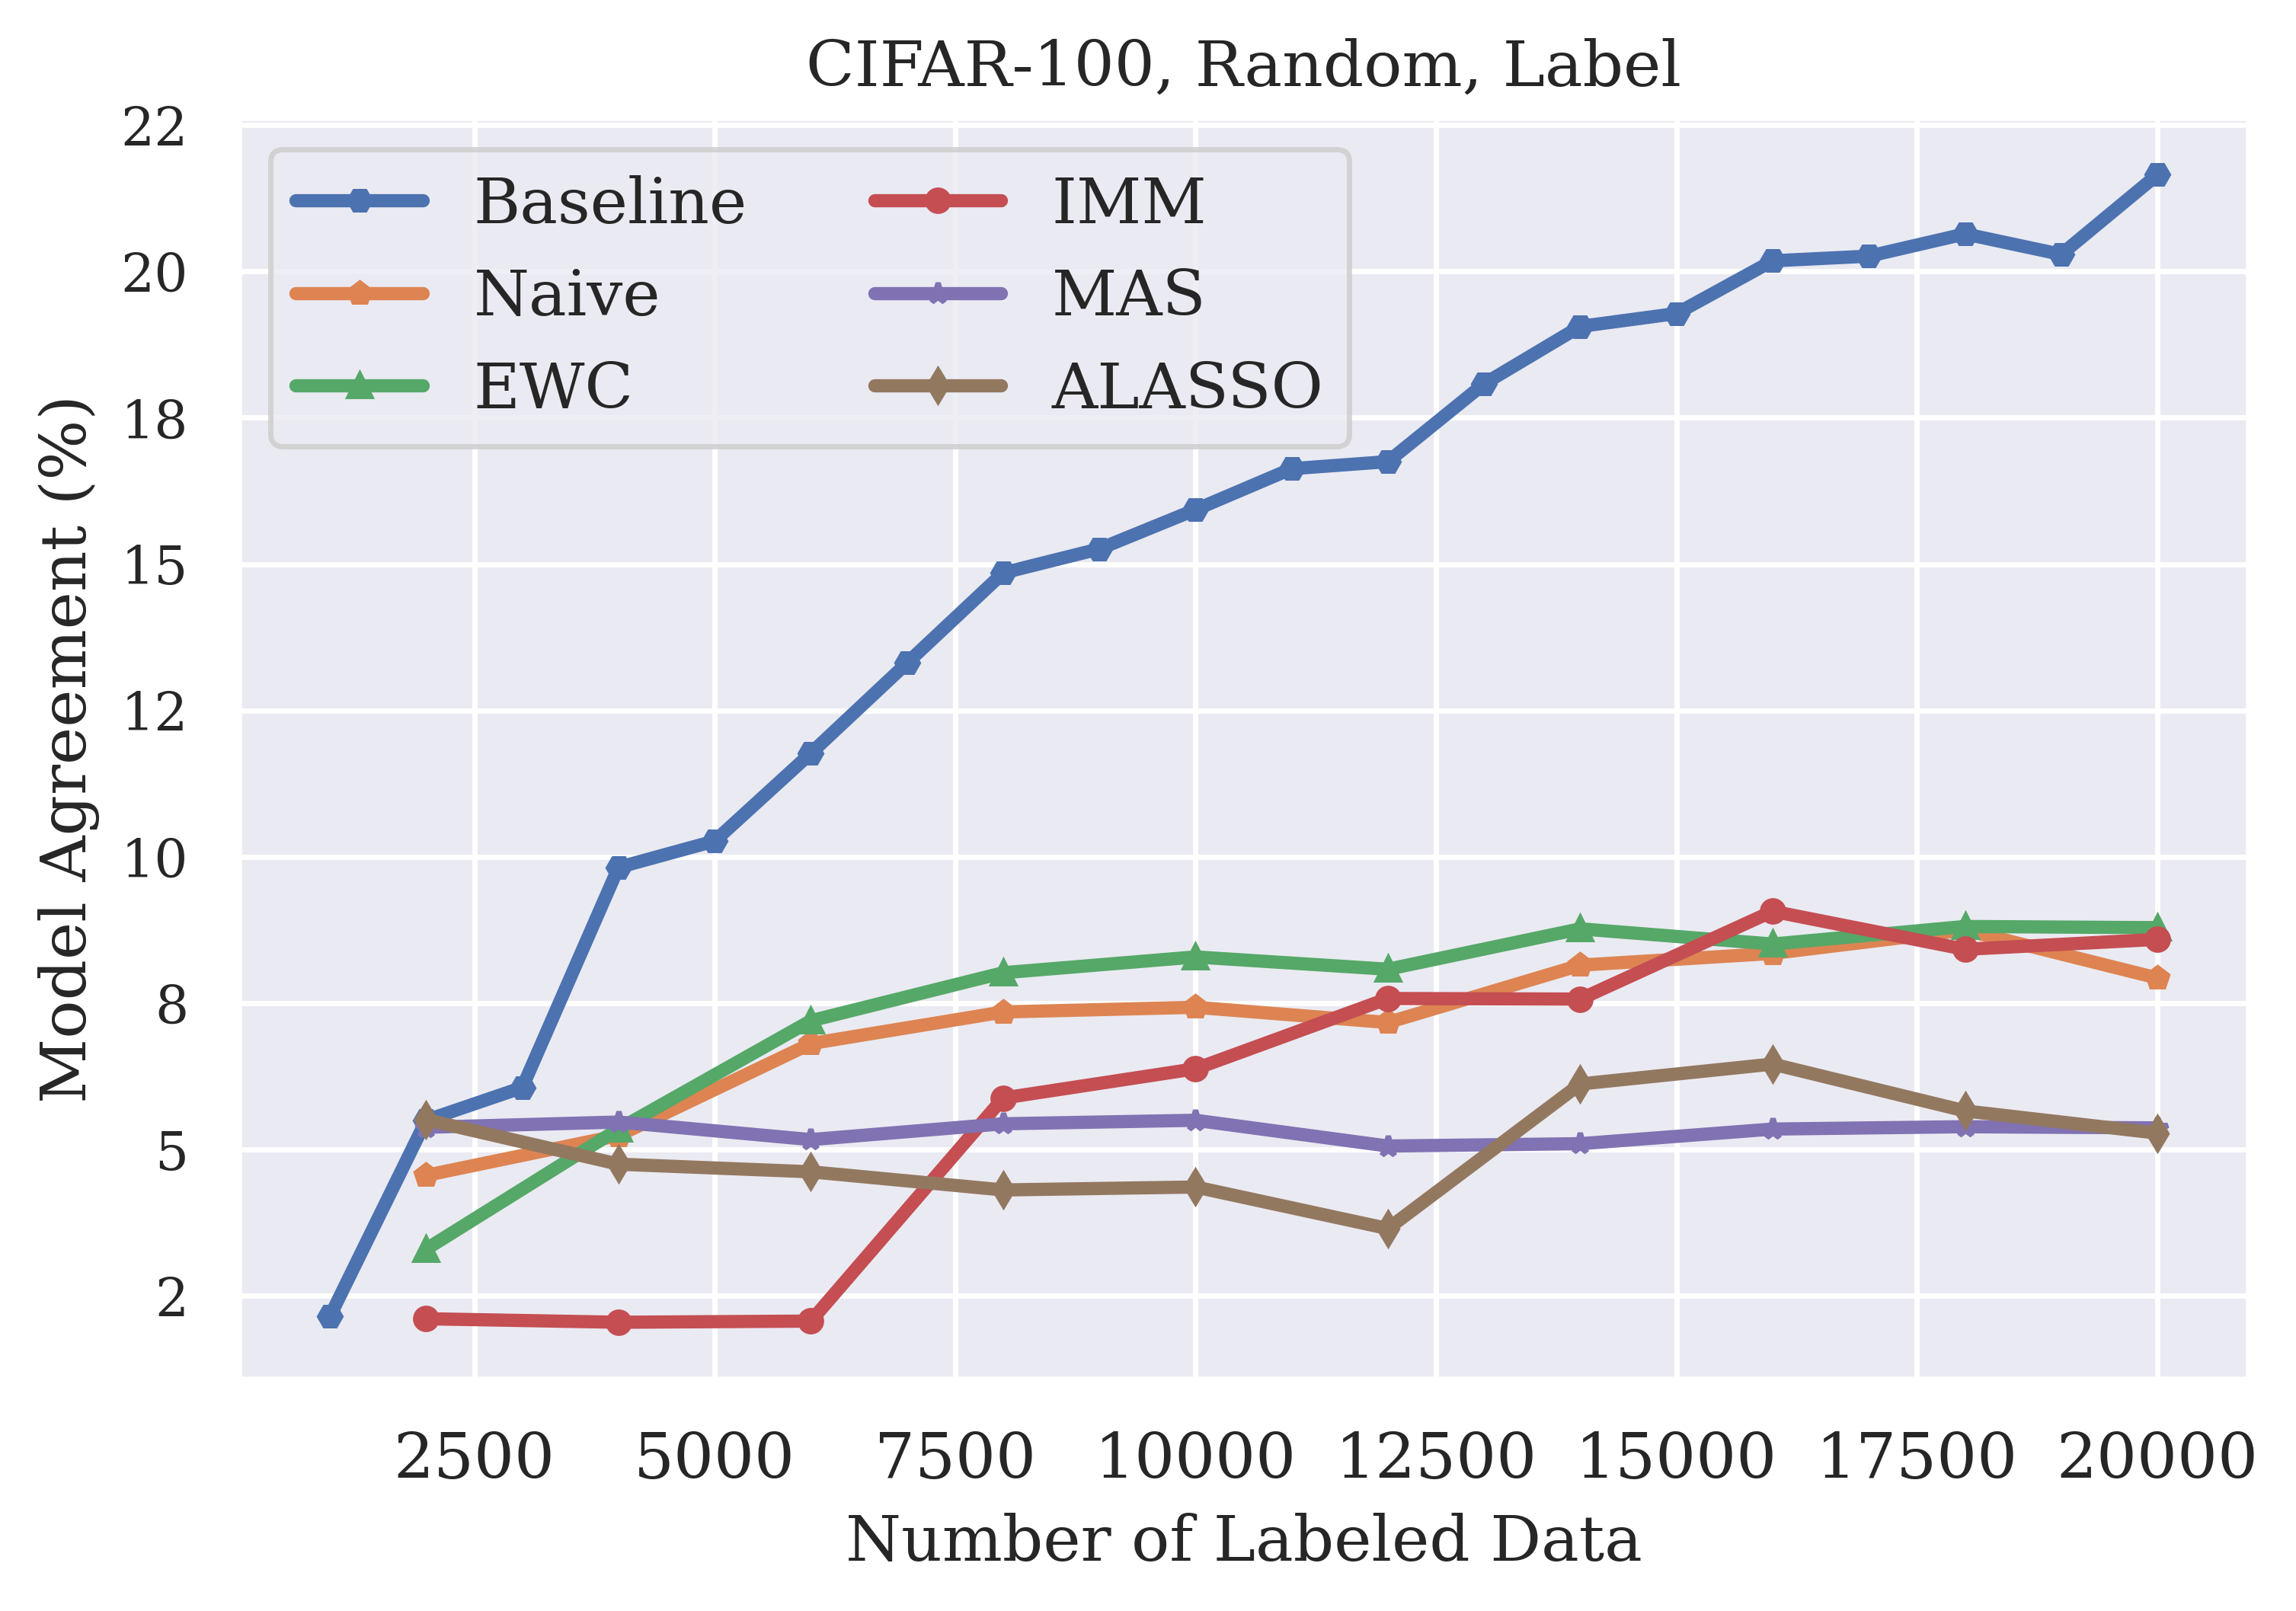
\includegraphics[width=0.48\linewidth]{images/results_CALMS/cifar100_label_random.png} \hfill
    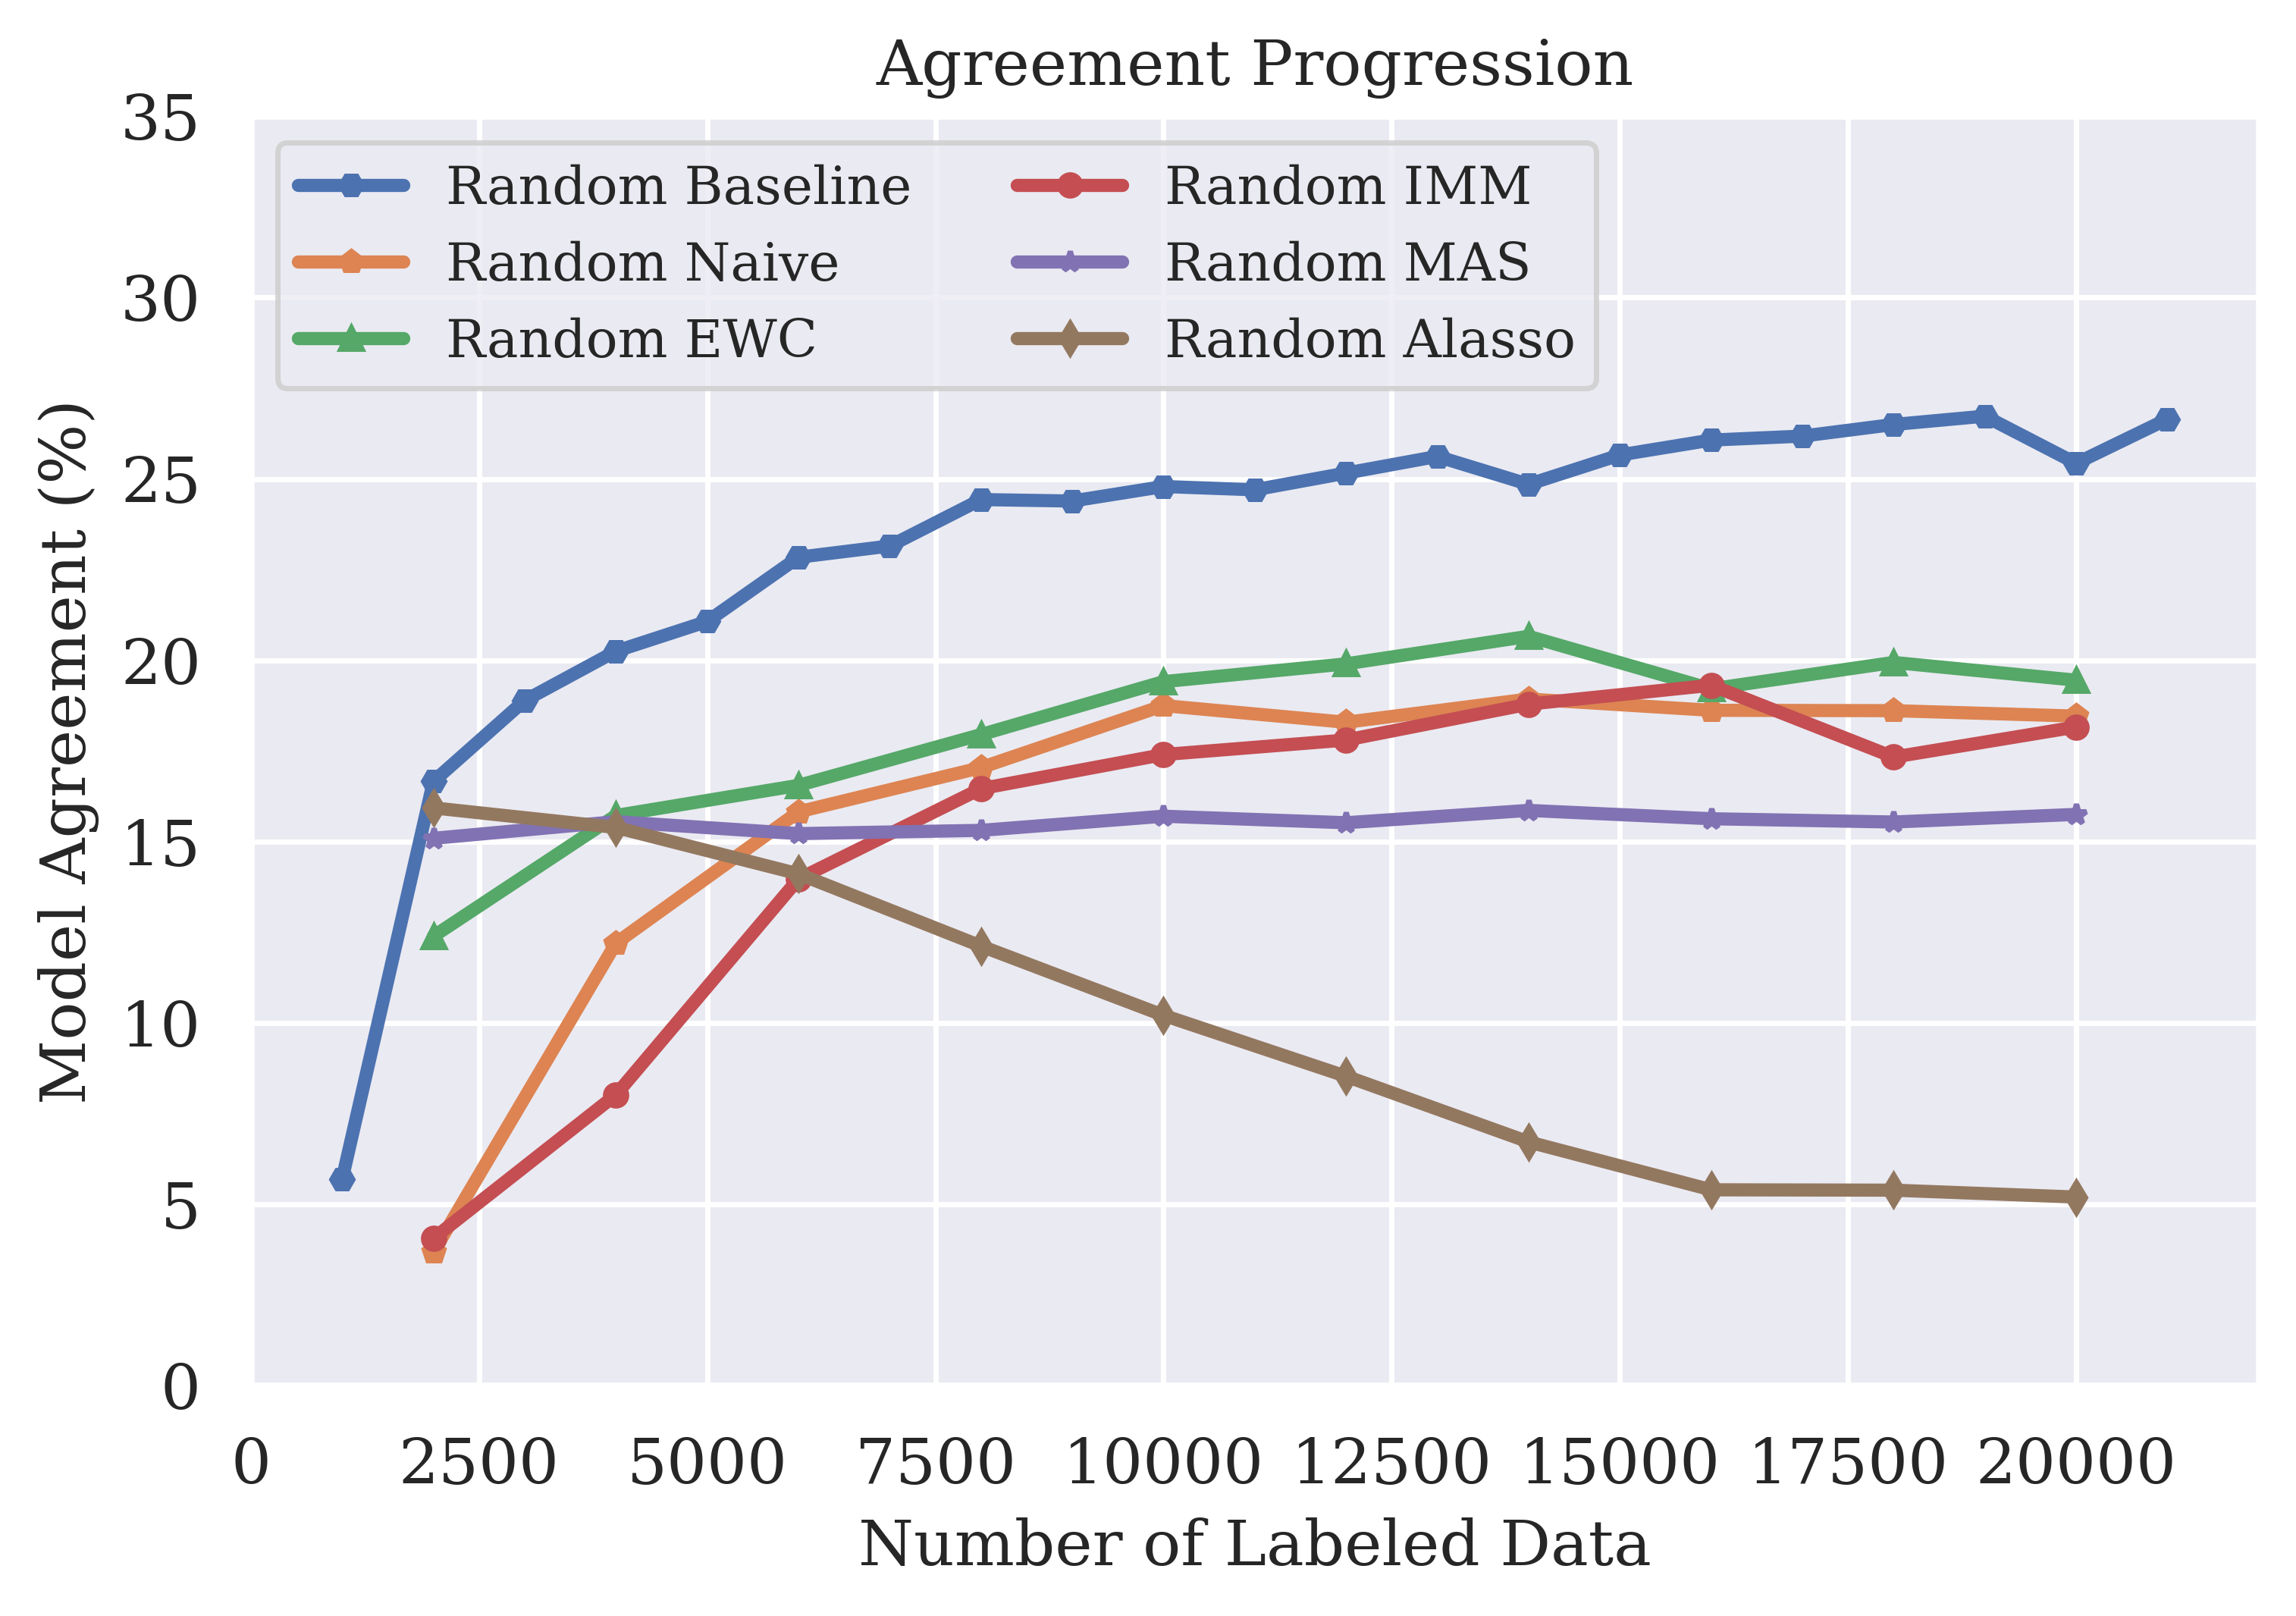
\includegraphics[width=0.48\linewidth]{images/results_CALMS/cifar100_softmax_random.png}
    \caption{Agreement comparison for model stealing on CIFAR-100 using the active learning strategy Random.}
    \label{fig:CALMSCIFAR100Random}
\end{figure}

\begin{figure}[!htb]
    \centering
    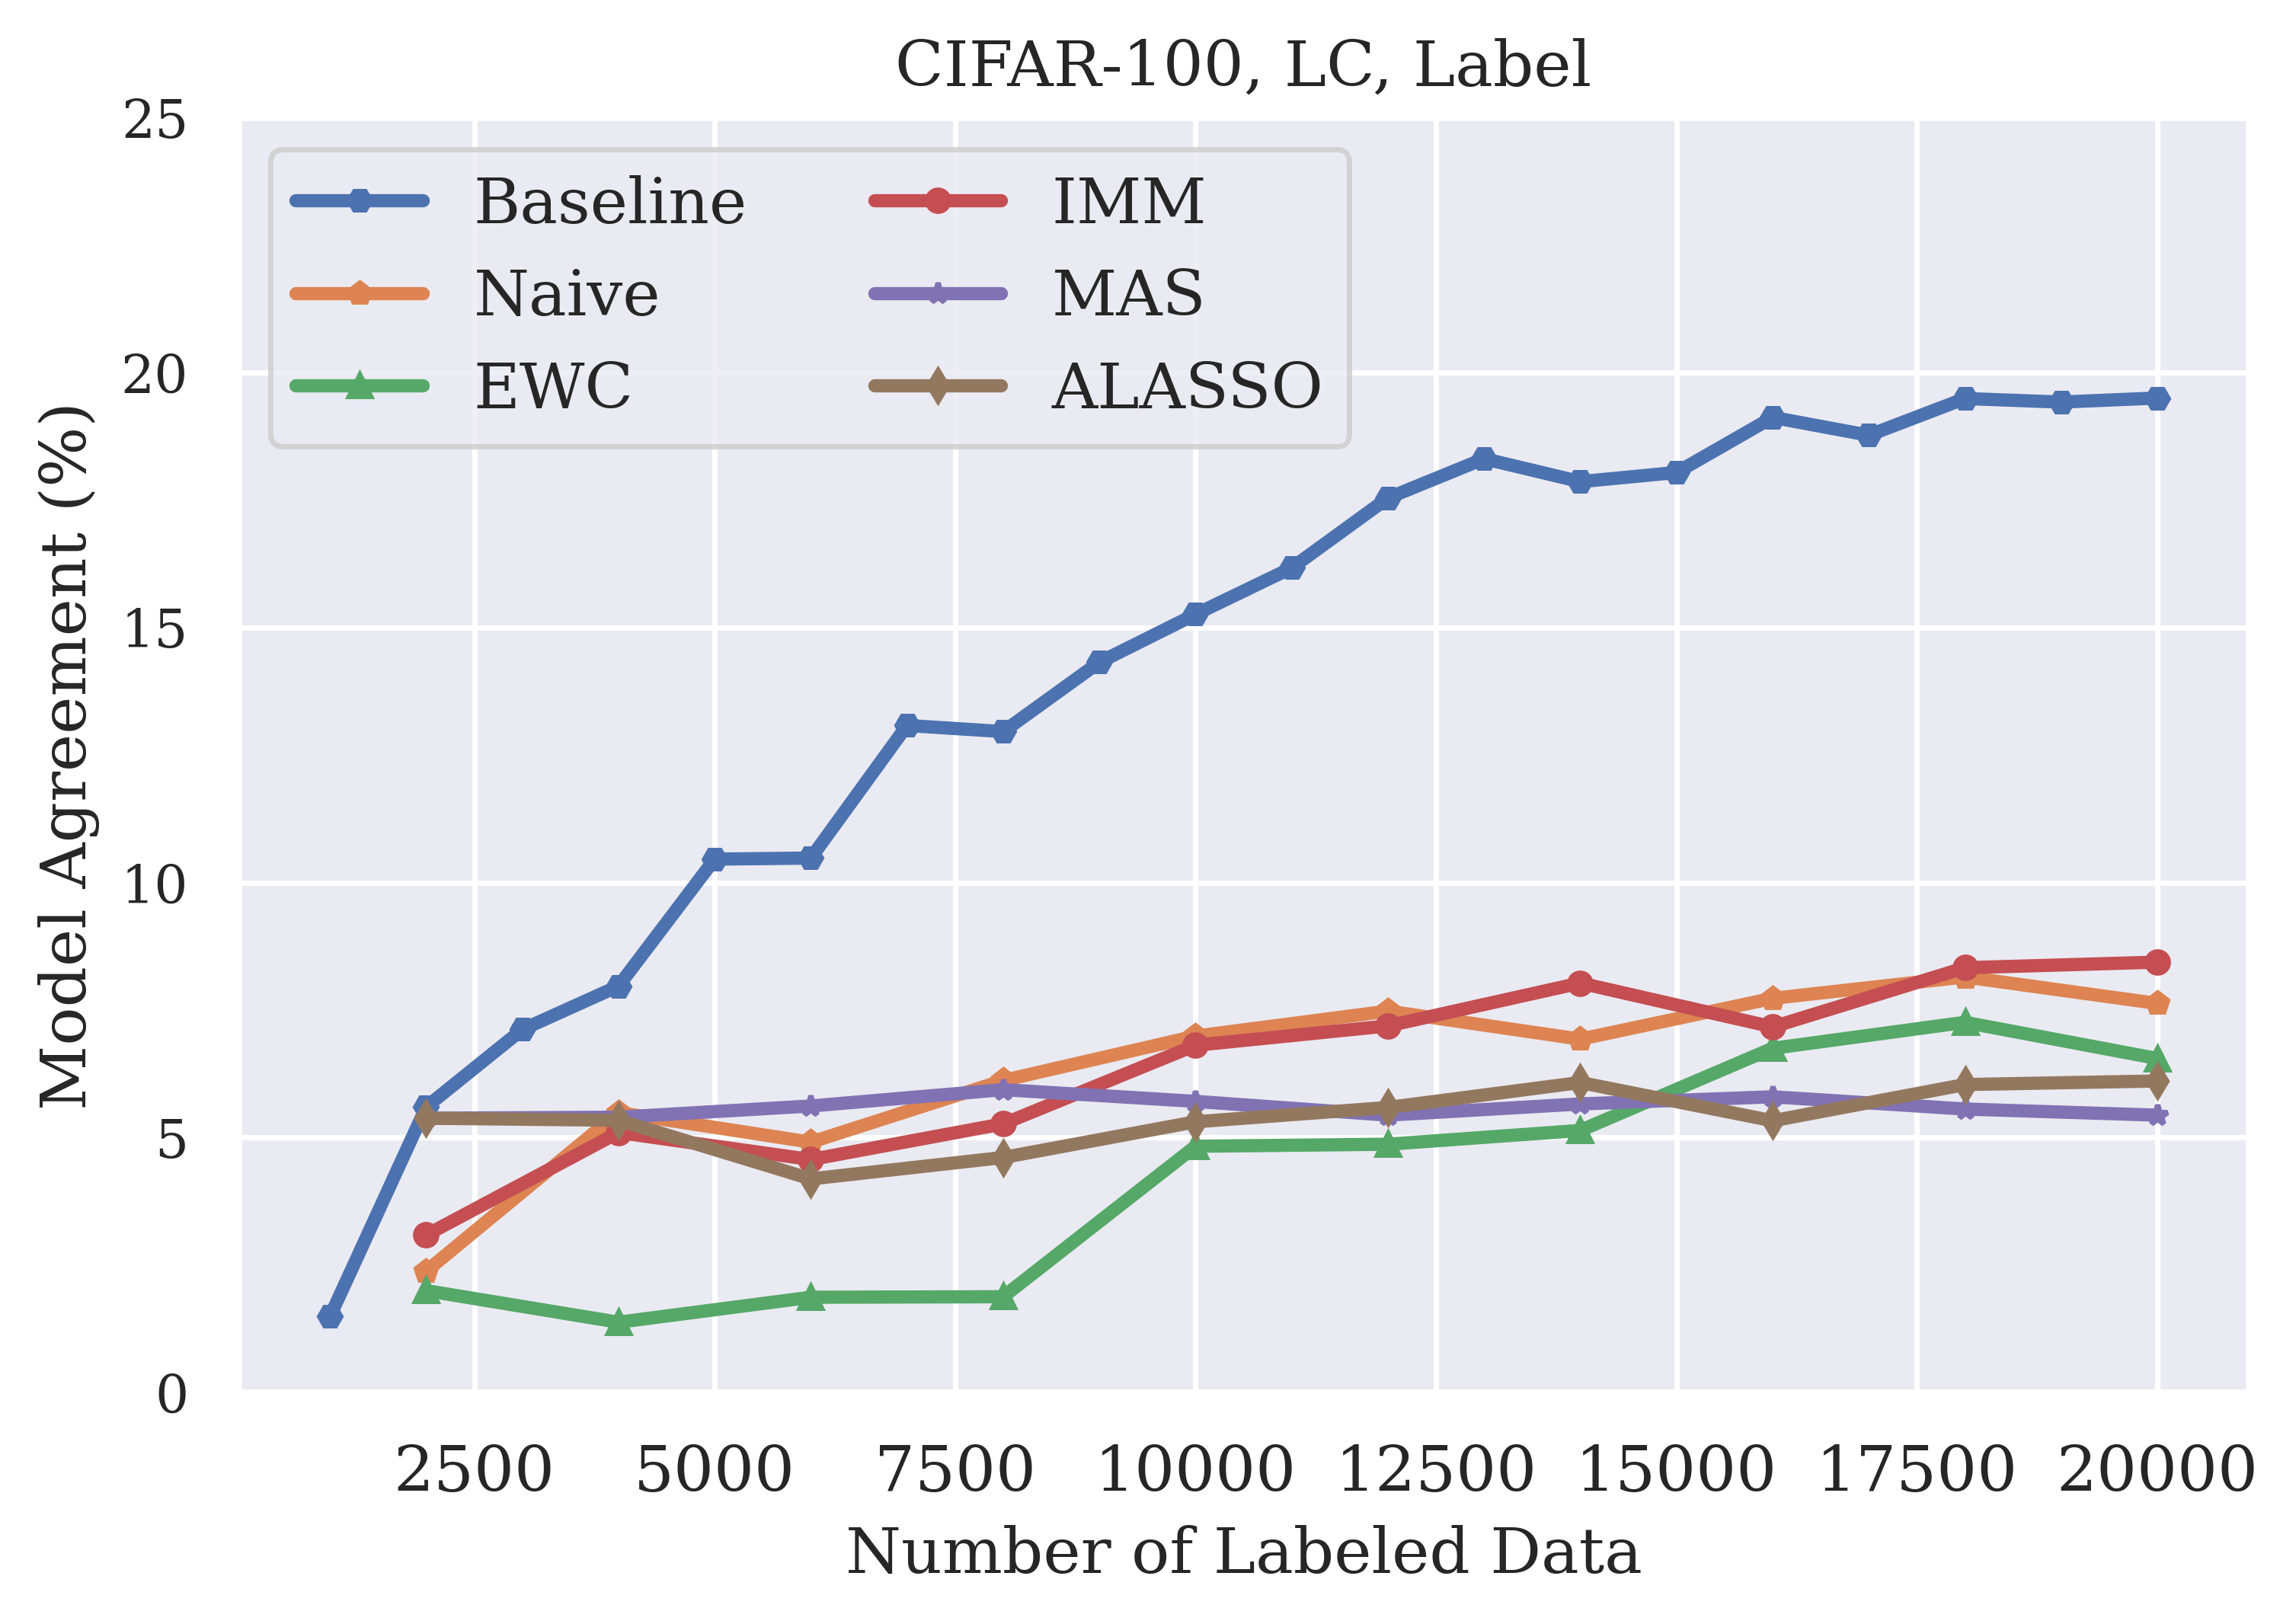
\includegraphics[width=0.48\linewidth]{images/results_CALMS/cifar100_label_lc.png} \hfill
    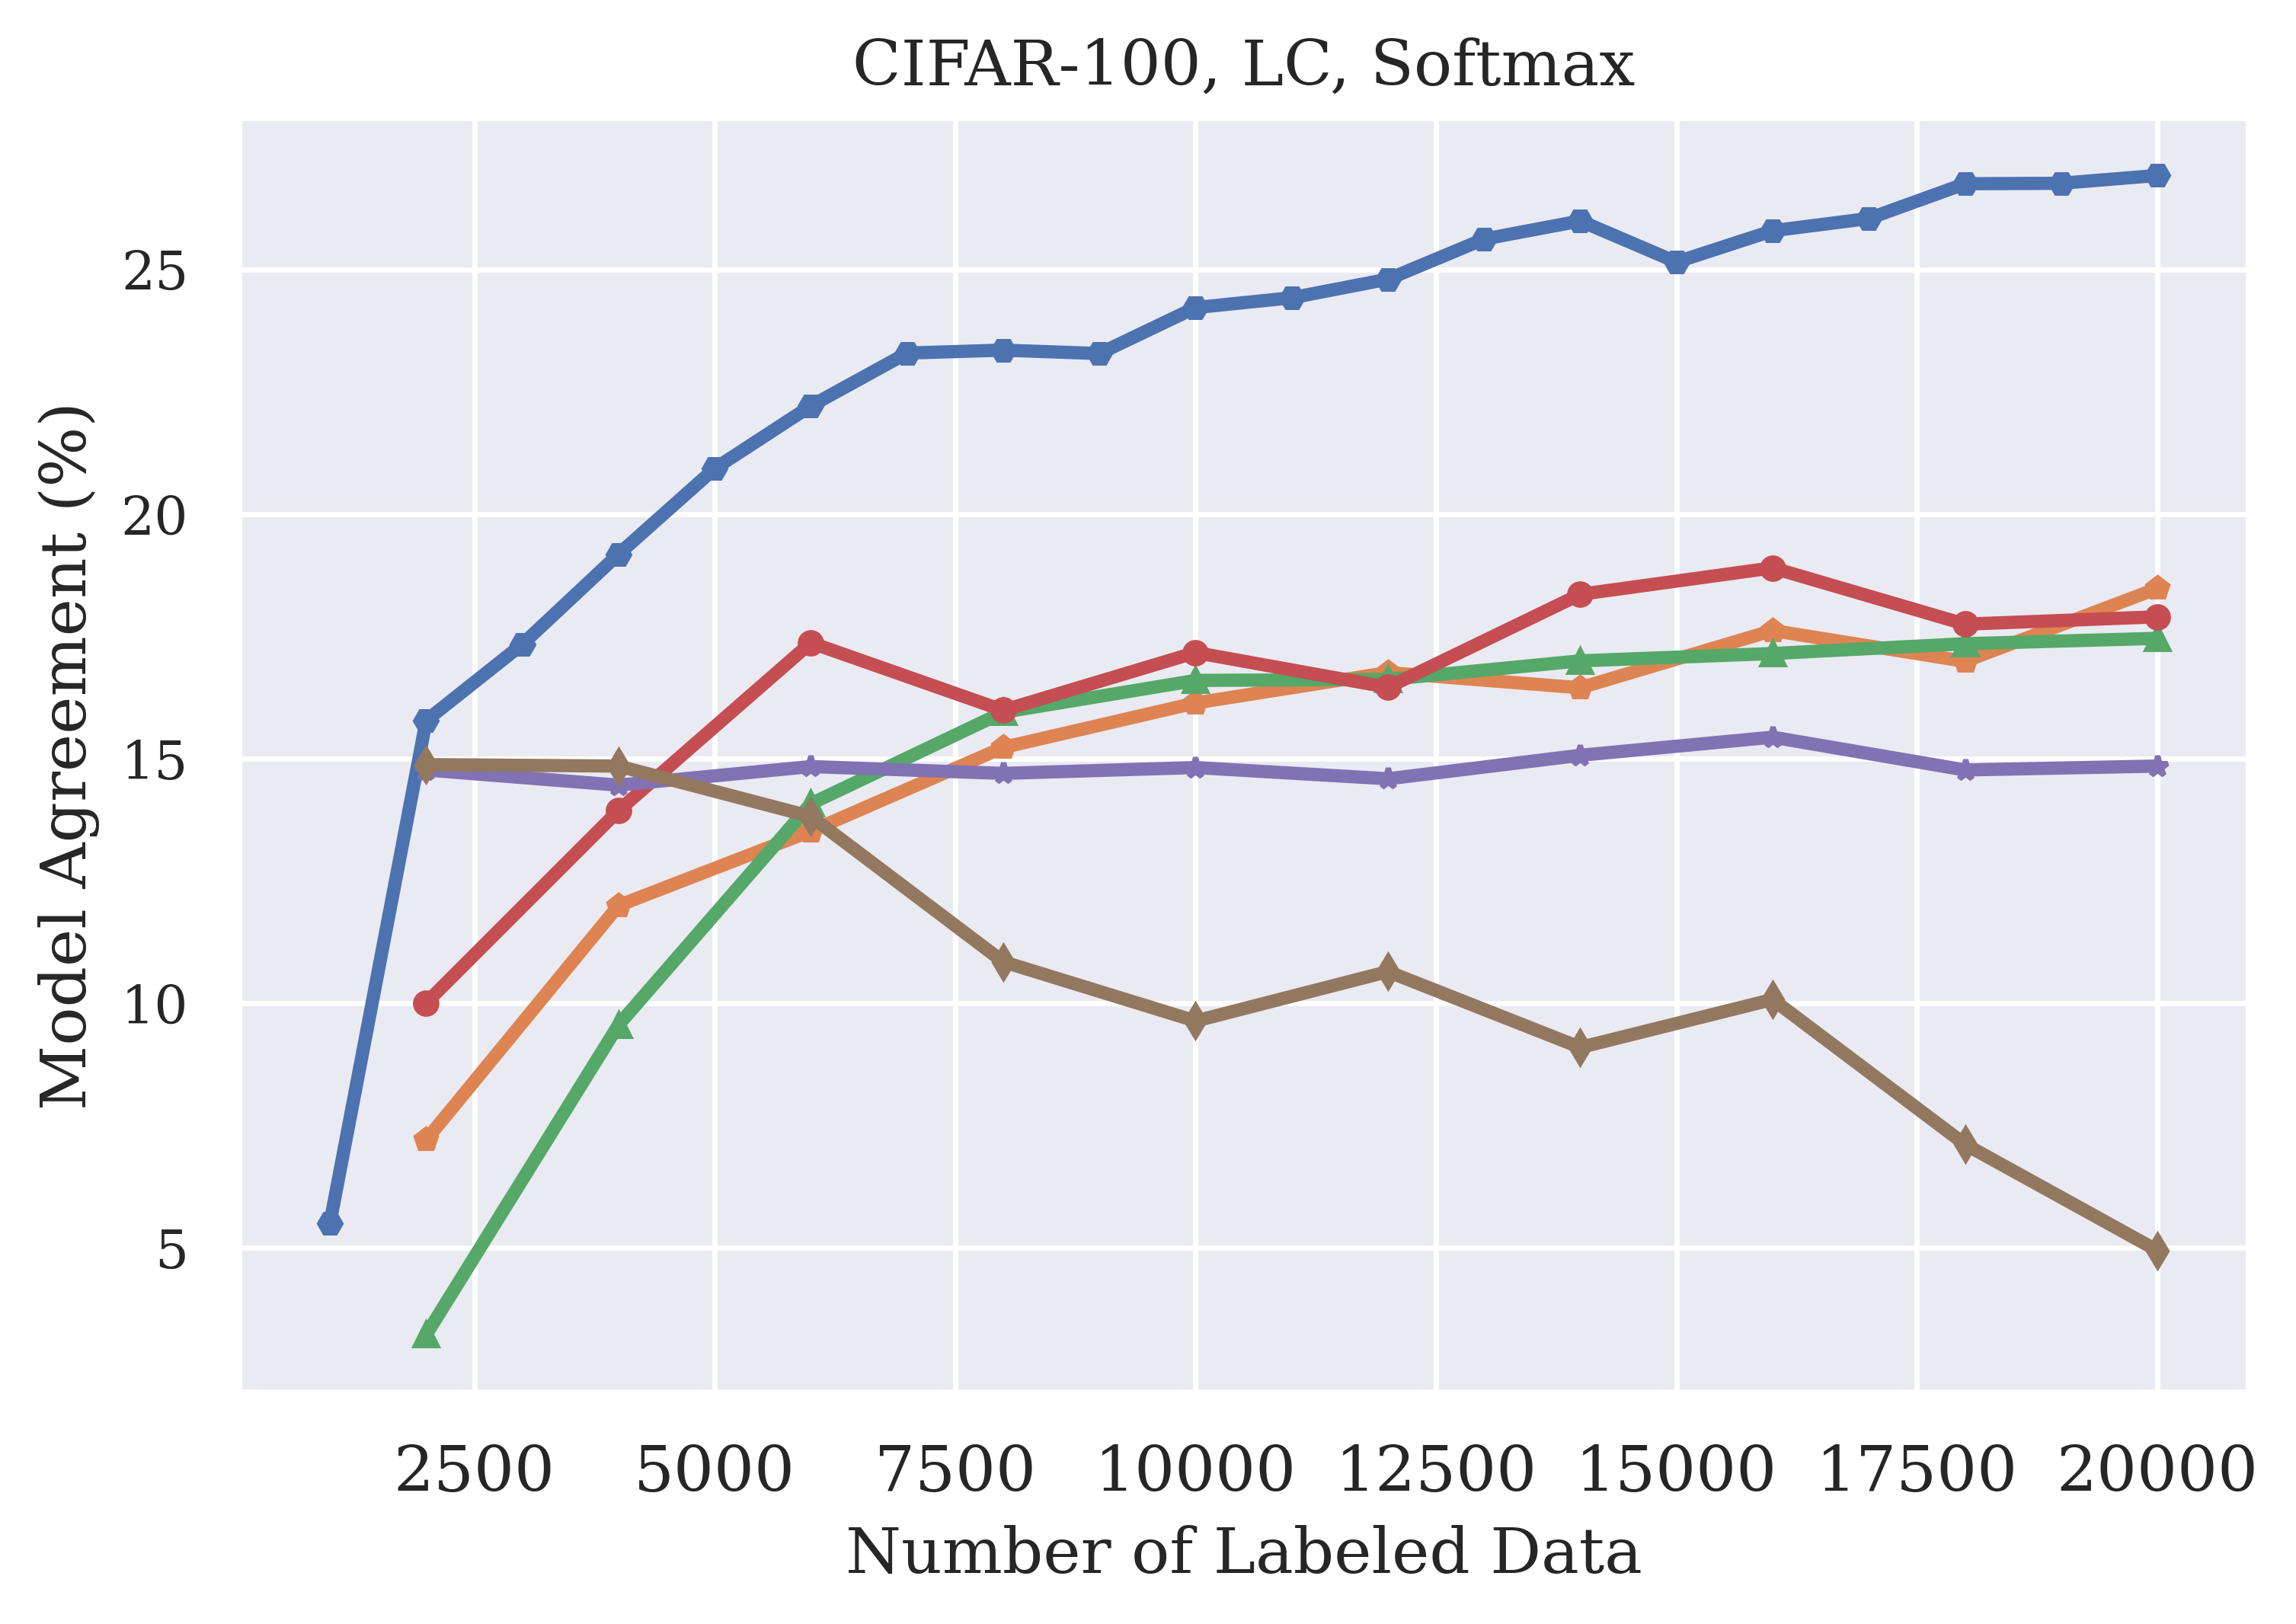
\includegraphics[width=0.48\linewidth]{images/results_CALMS/cifar100_softmax_lc.png}
    \caption{Agreement comparison for model stealing on CIFAR-100 using the active learning strategy \gls{lc}.}
    \label{fig:CALMSCIFAR100LC}
\end{figure}

\begin{figure}[!htb]
    \centering
    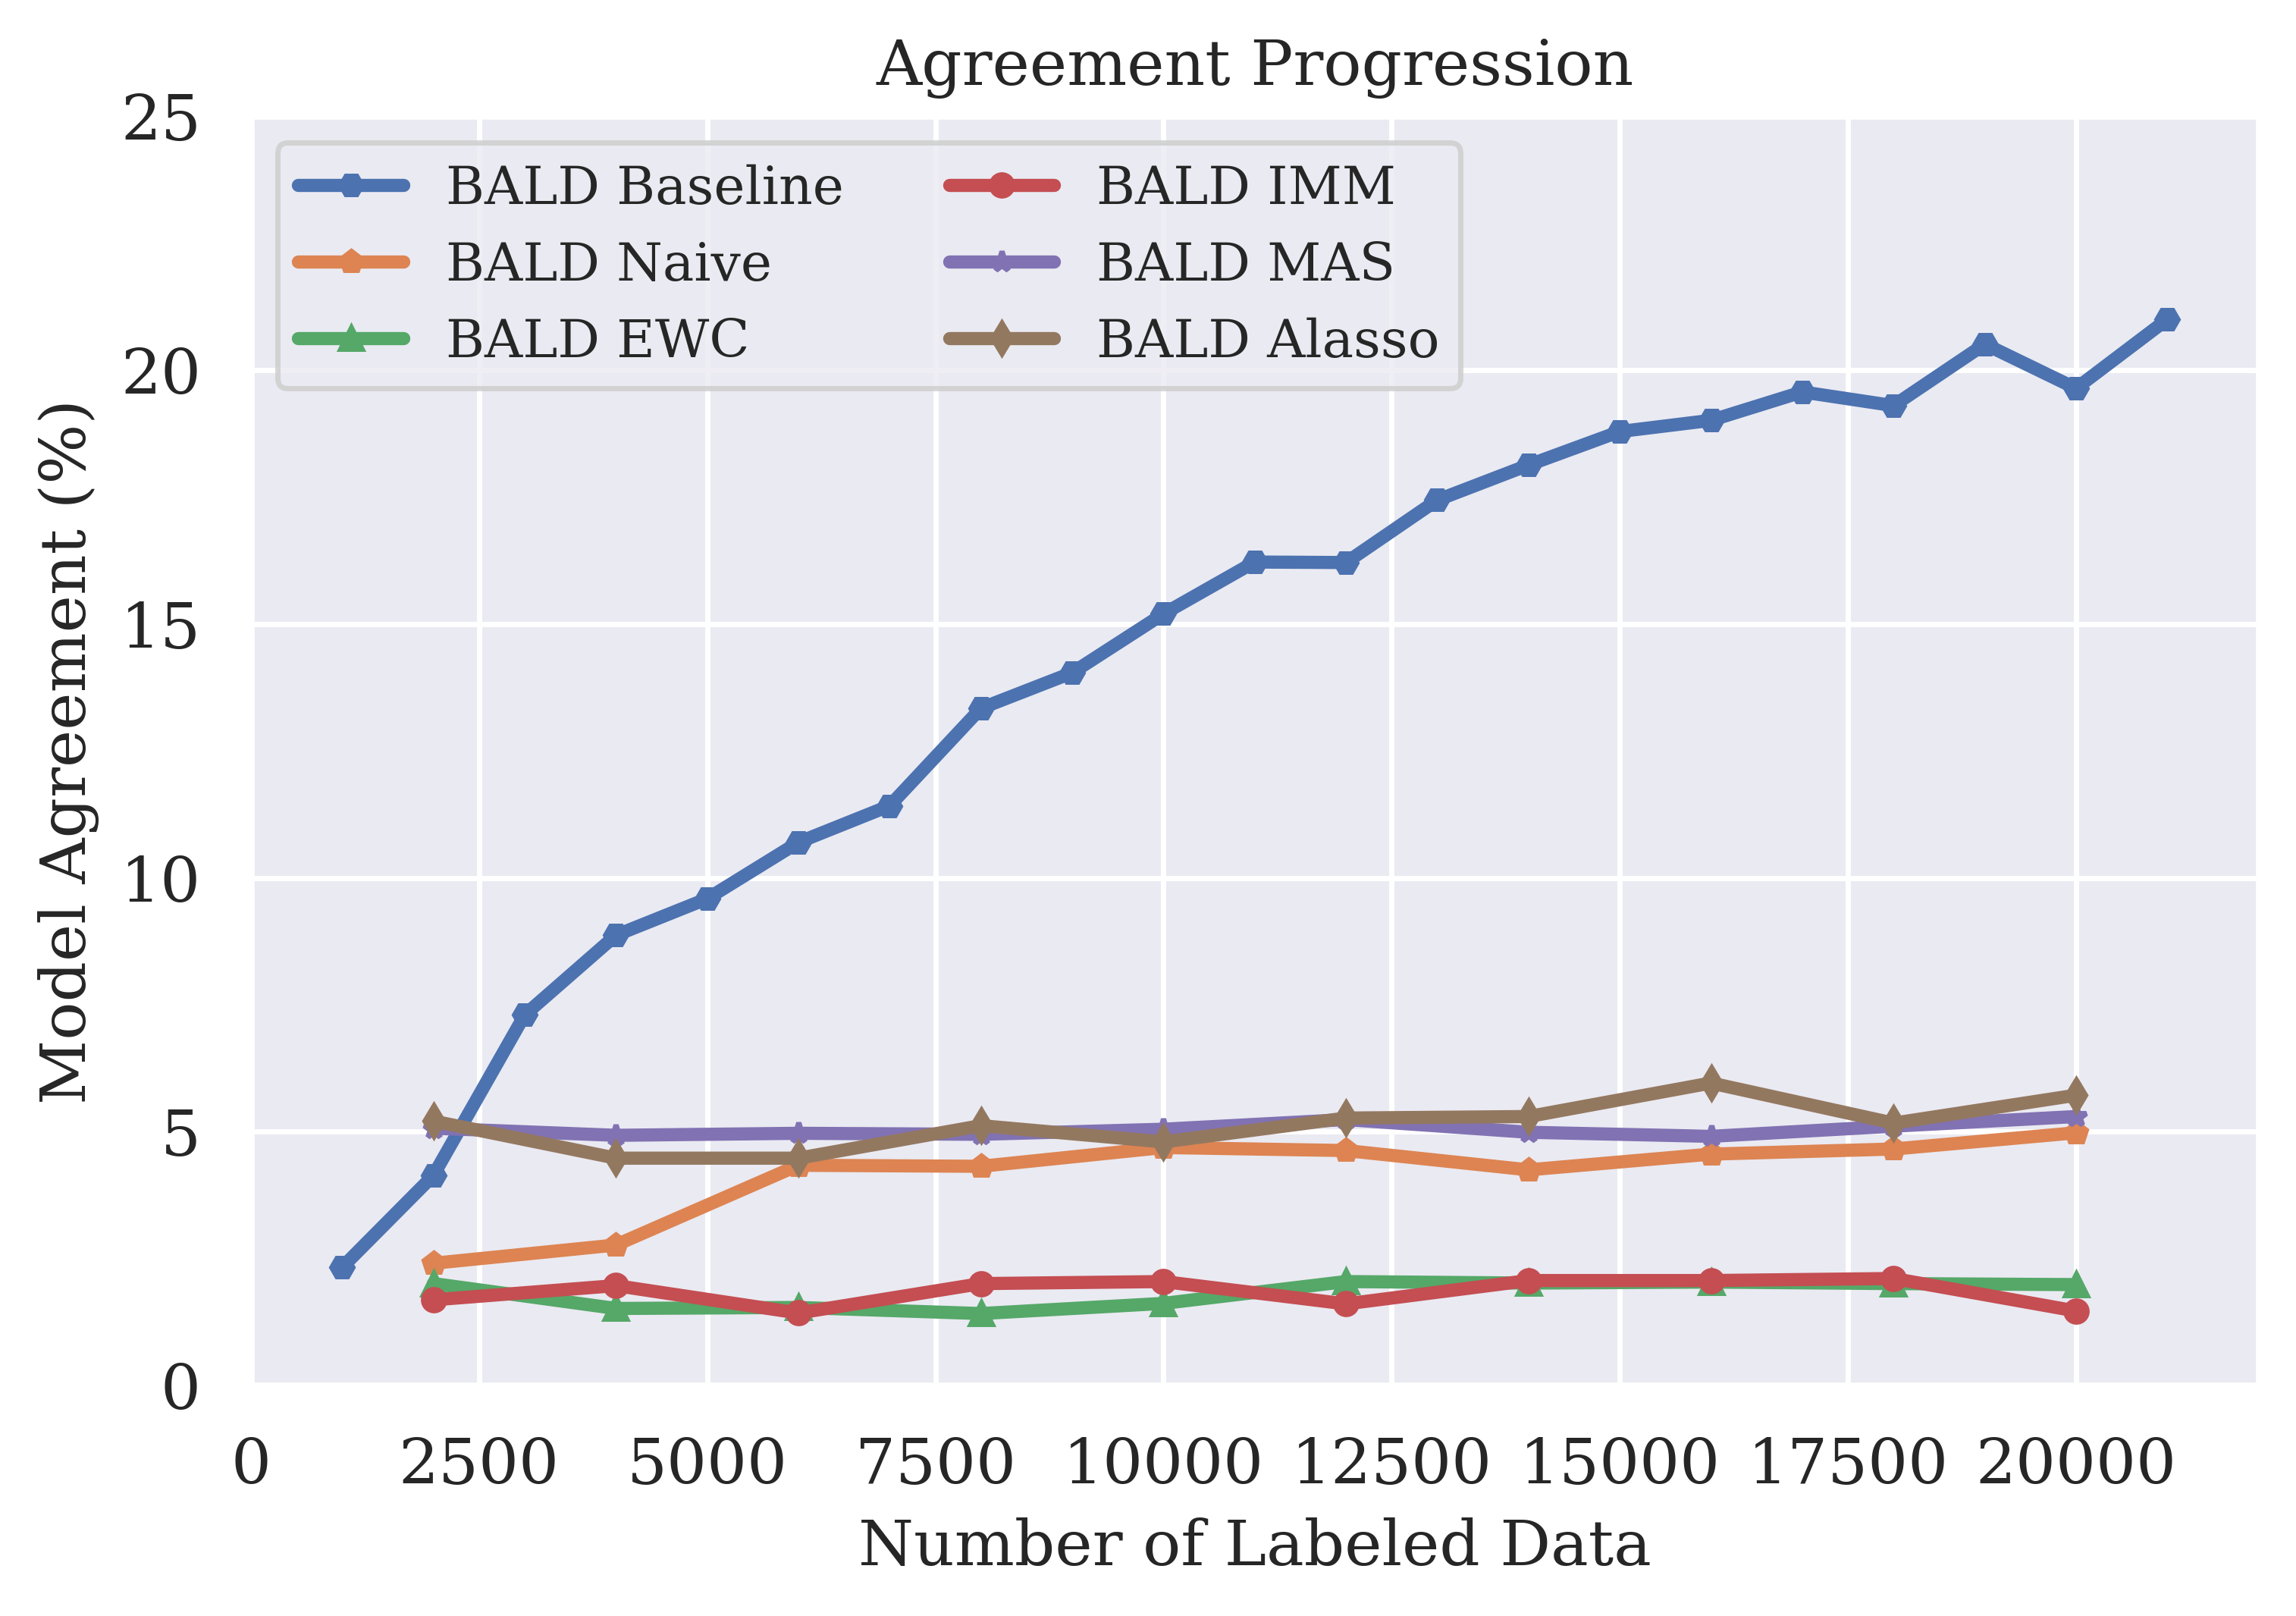
\includegraphics[width=0.48\linewidth]{images/results_CALMS/cifar100_label_bald.png} \hfill
    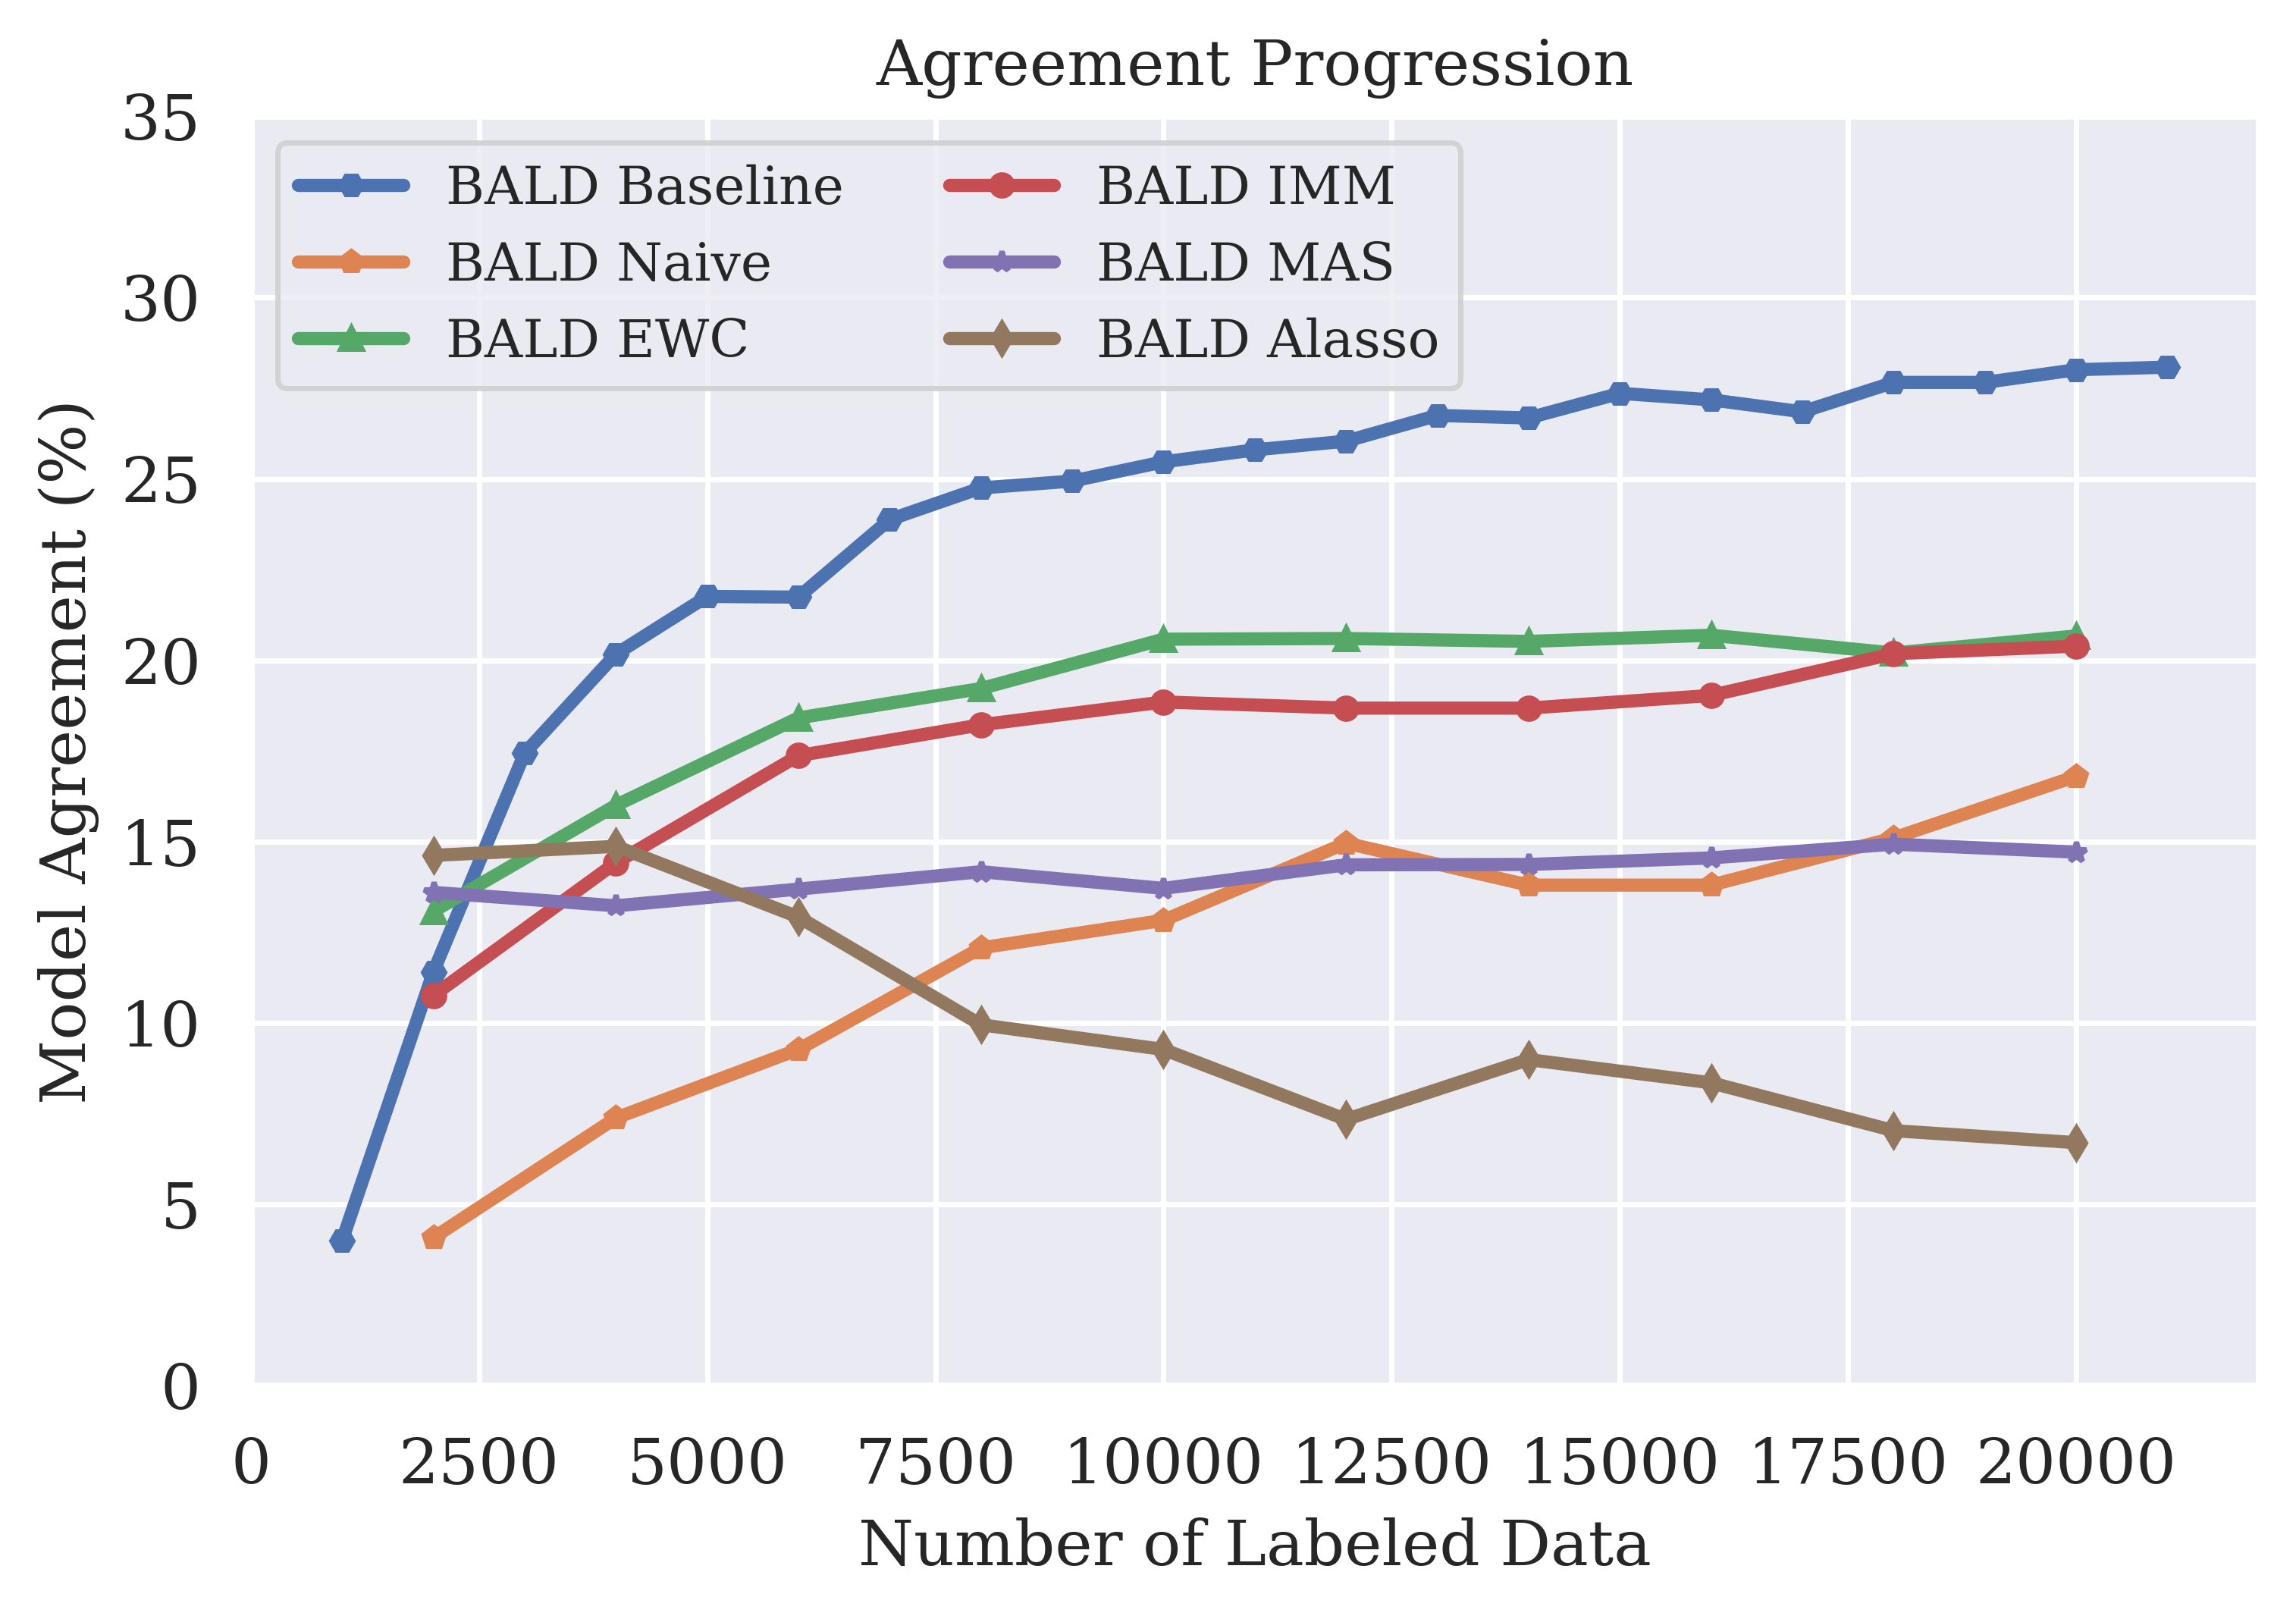
\includegraphics[width=0.48\linewidth]{images/results_CALMS/cifar100_softmax_bald.png}
    \caption{Agreement comparison for model stealing on CIFAR-100 using the active learning strategy \gls{bald}.}
    \label{fig:CALMSCIFAR100BALD}
\end{figure}

\begin{figure}[!htb]
    \centering
    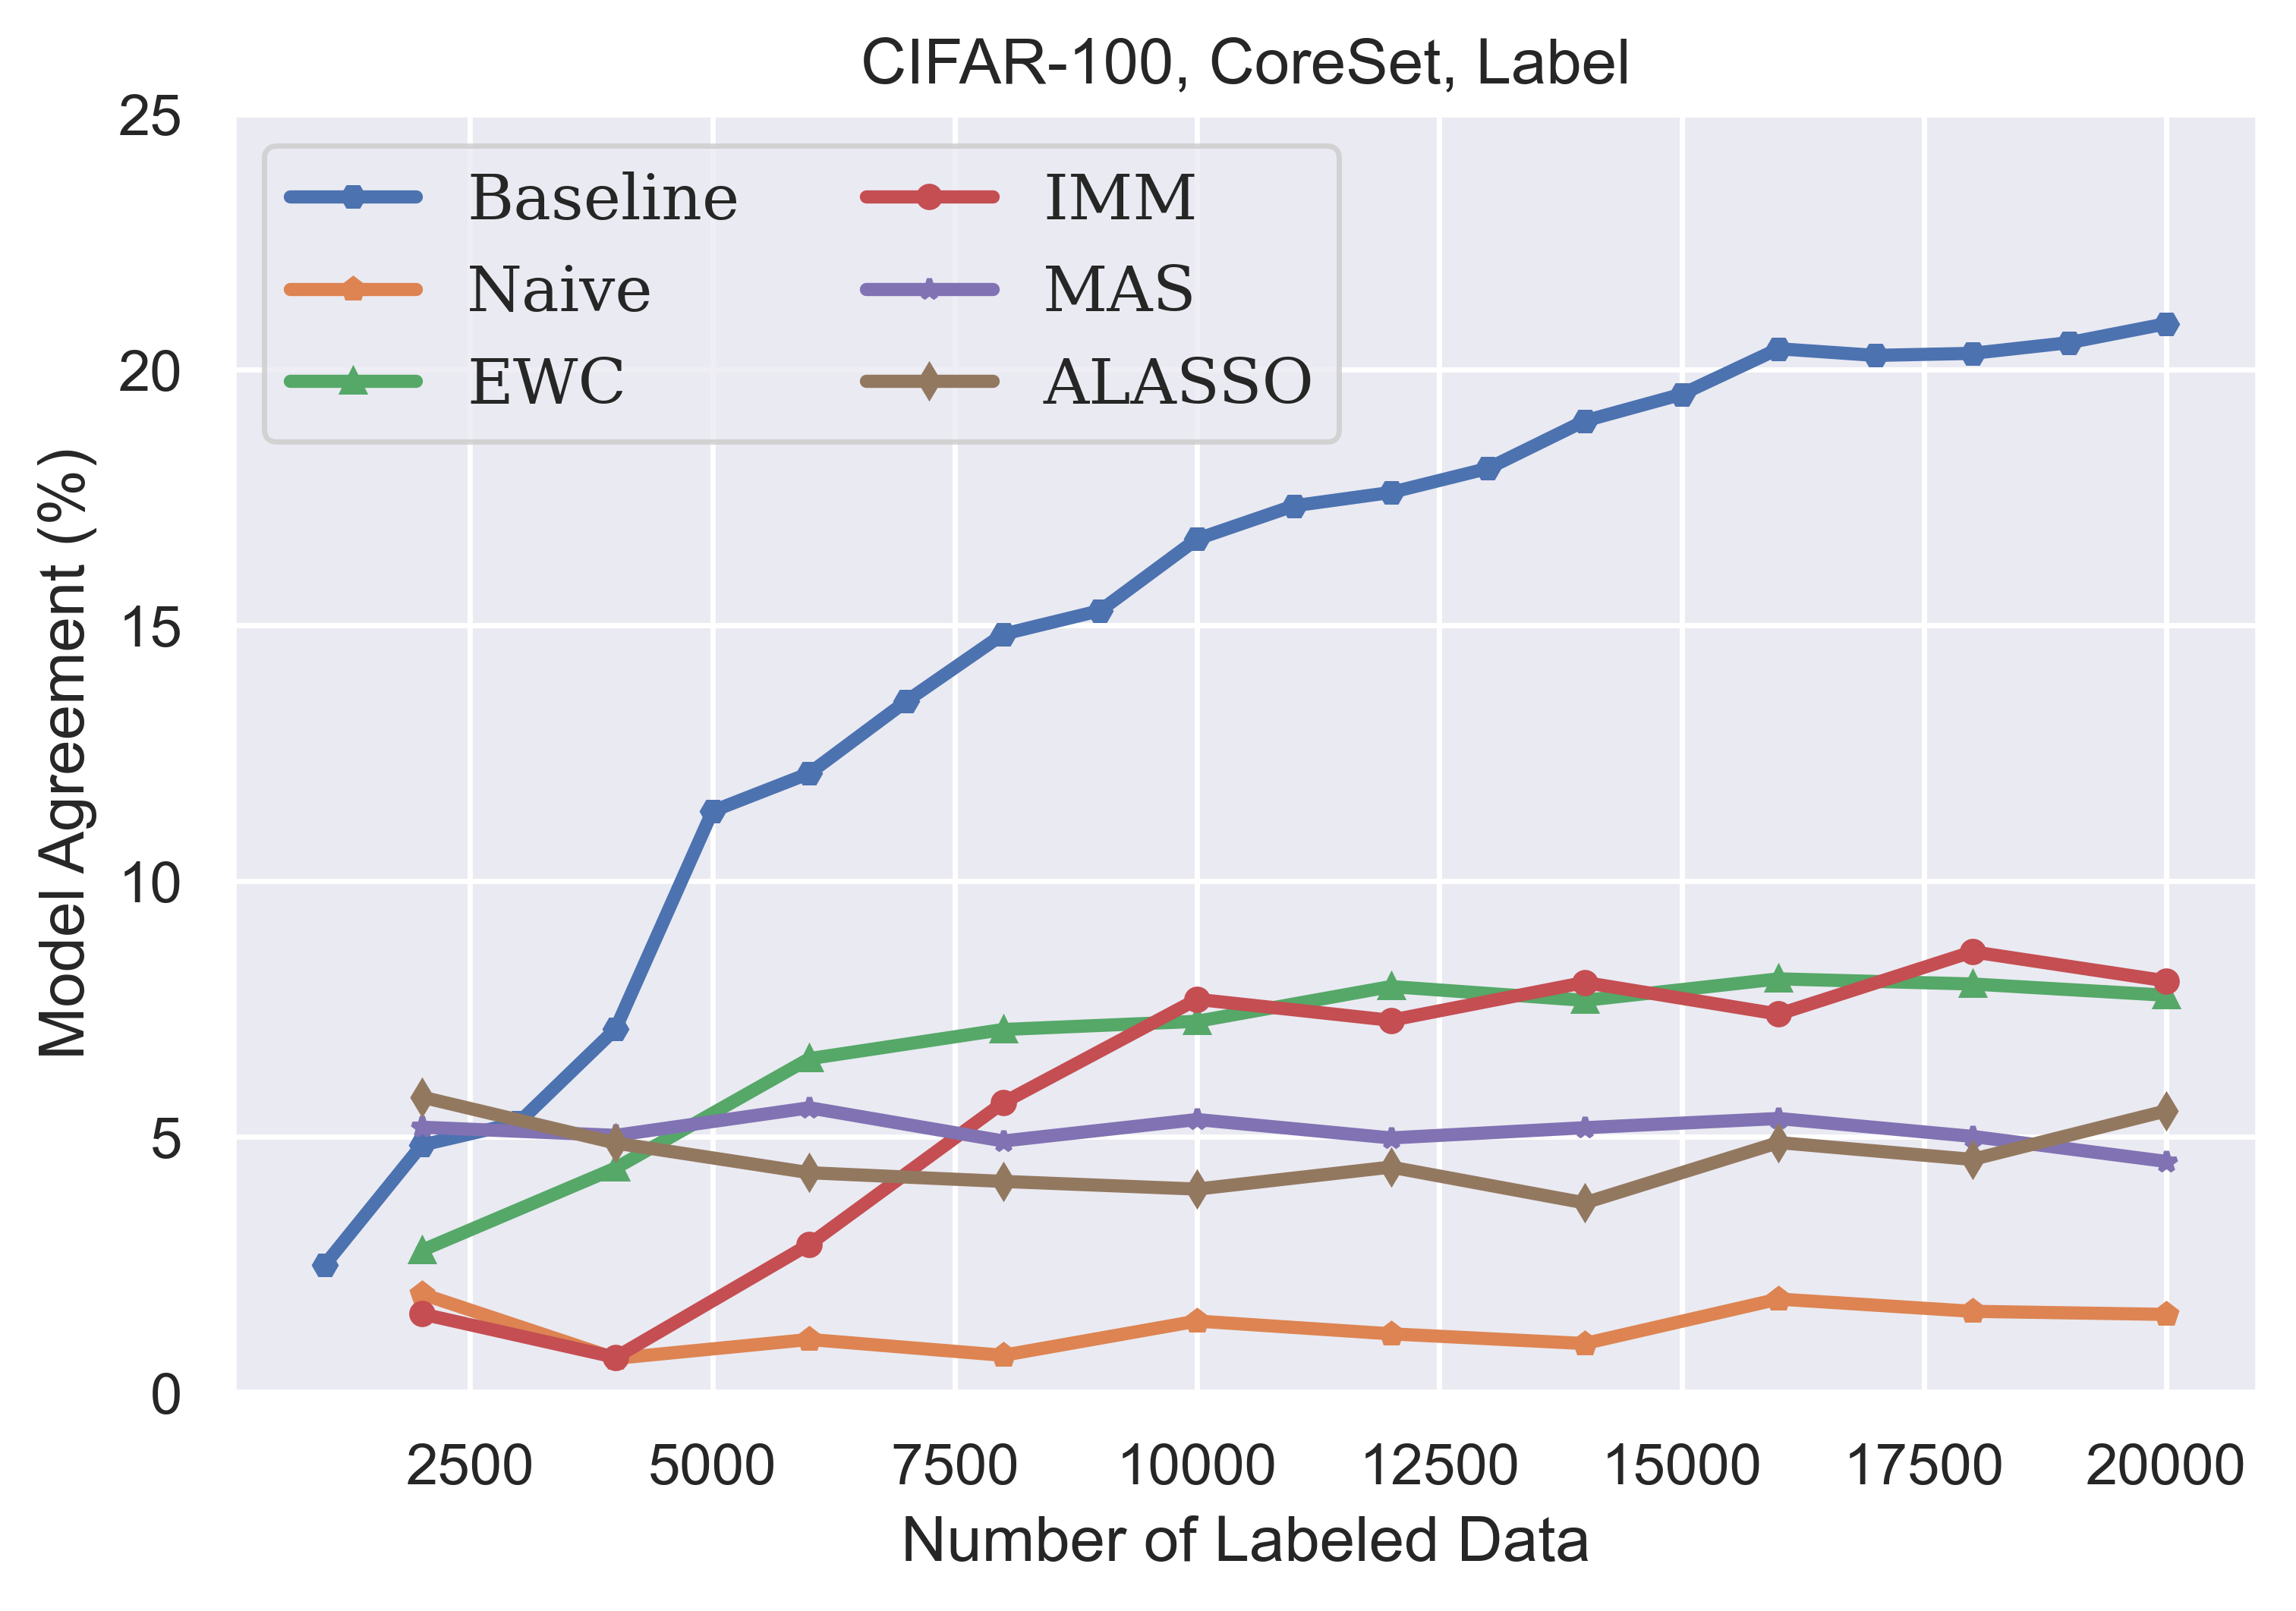
\includegraphics[width=0.48\linewidth]{images/results_CALMS/cifar100_label_coreset.png} \hfill
    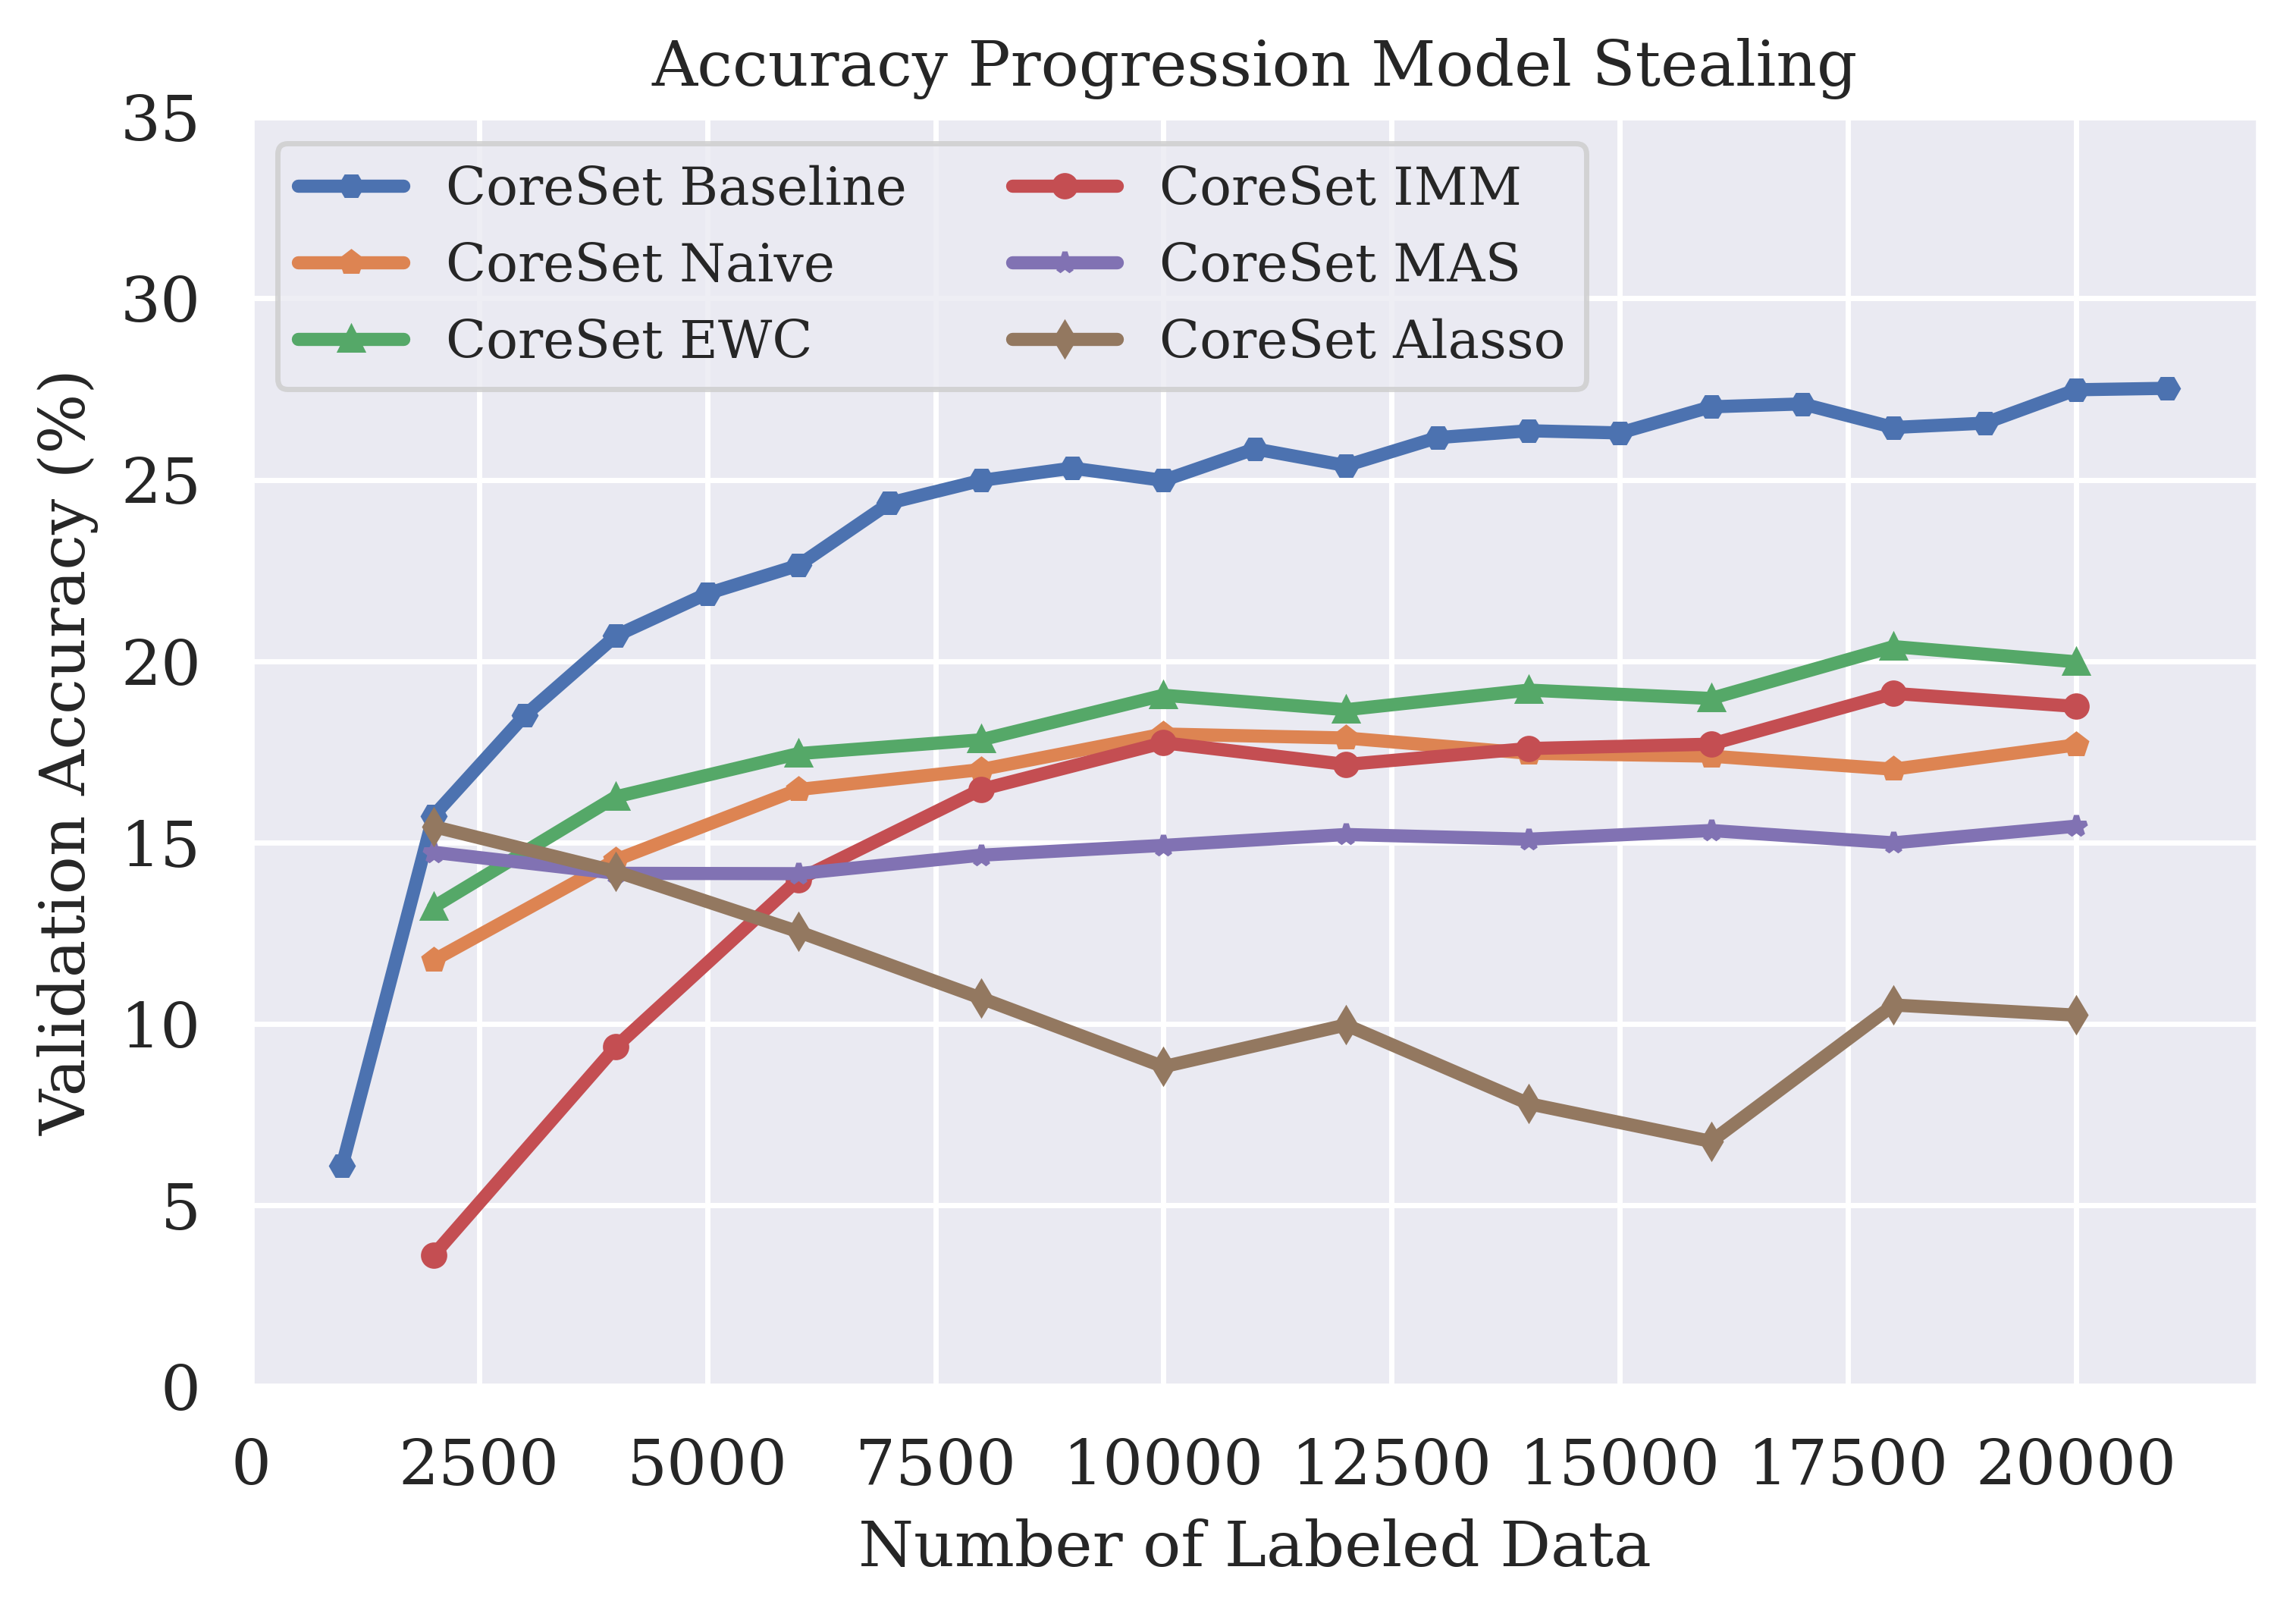
\includegraphics[width=0.48\linewidth]{images/results_CALMS/cifar100_softmax_coreset.png}
    \caption{Agreement comparison for model stealing on CIFAR-100 using the active learning strategy CoreSet.}
    \label{fig:CALMSCIFAR100CoreSet}
\end{figure}

\clearpage

\subsubsection{VAAL and A-GEM}
\label{sec:Appendix:CALMS:VAALAGEM}
In the following we list the complete results for the experiments using \gls{vaal} and \gls{a-gem} on the datasets MNIST, CIFAR-10 and CIFAR-100.
\begin{figure}[!htb]
    \centering
    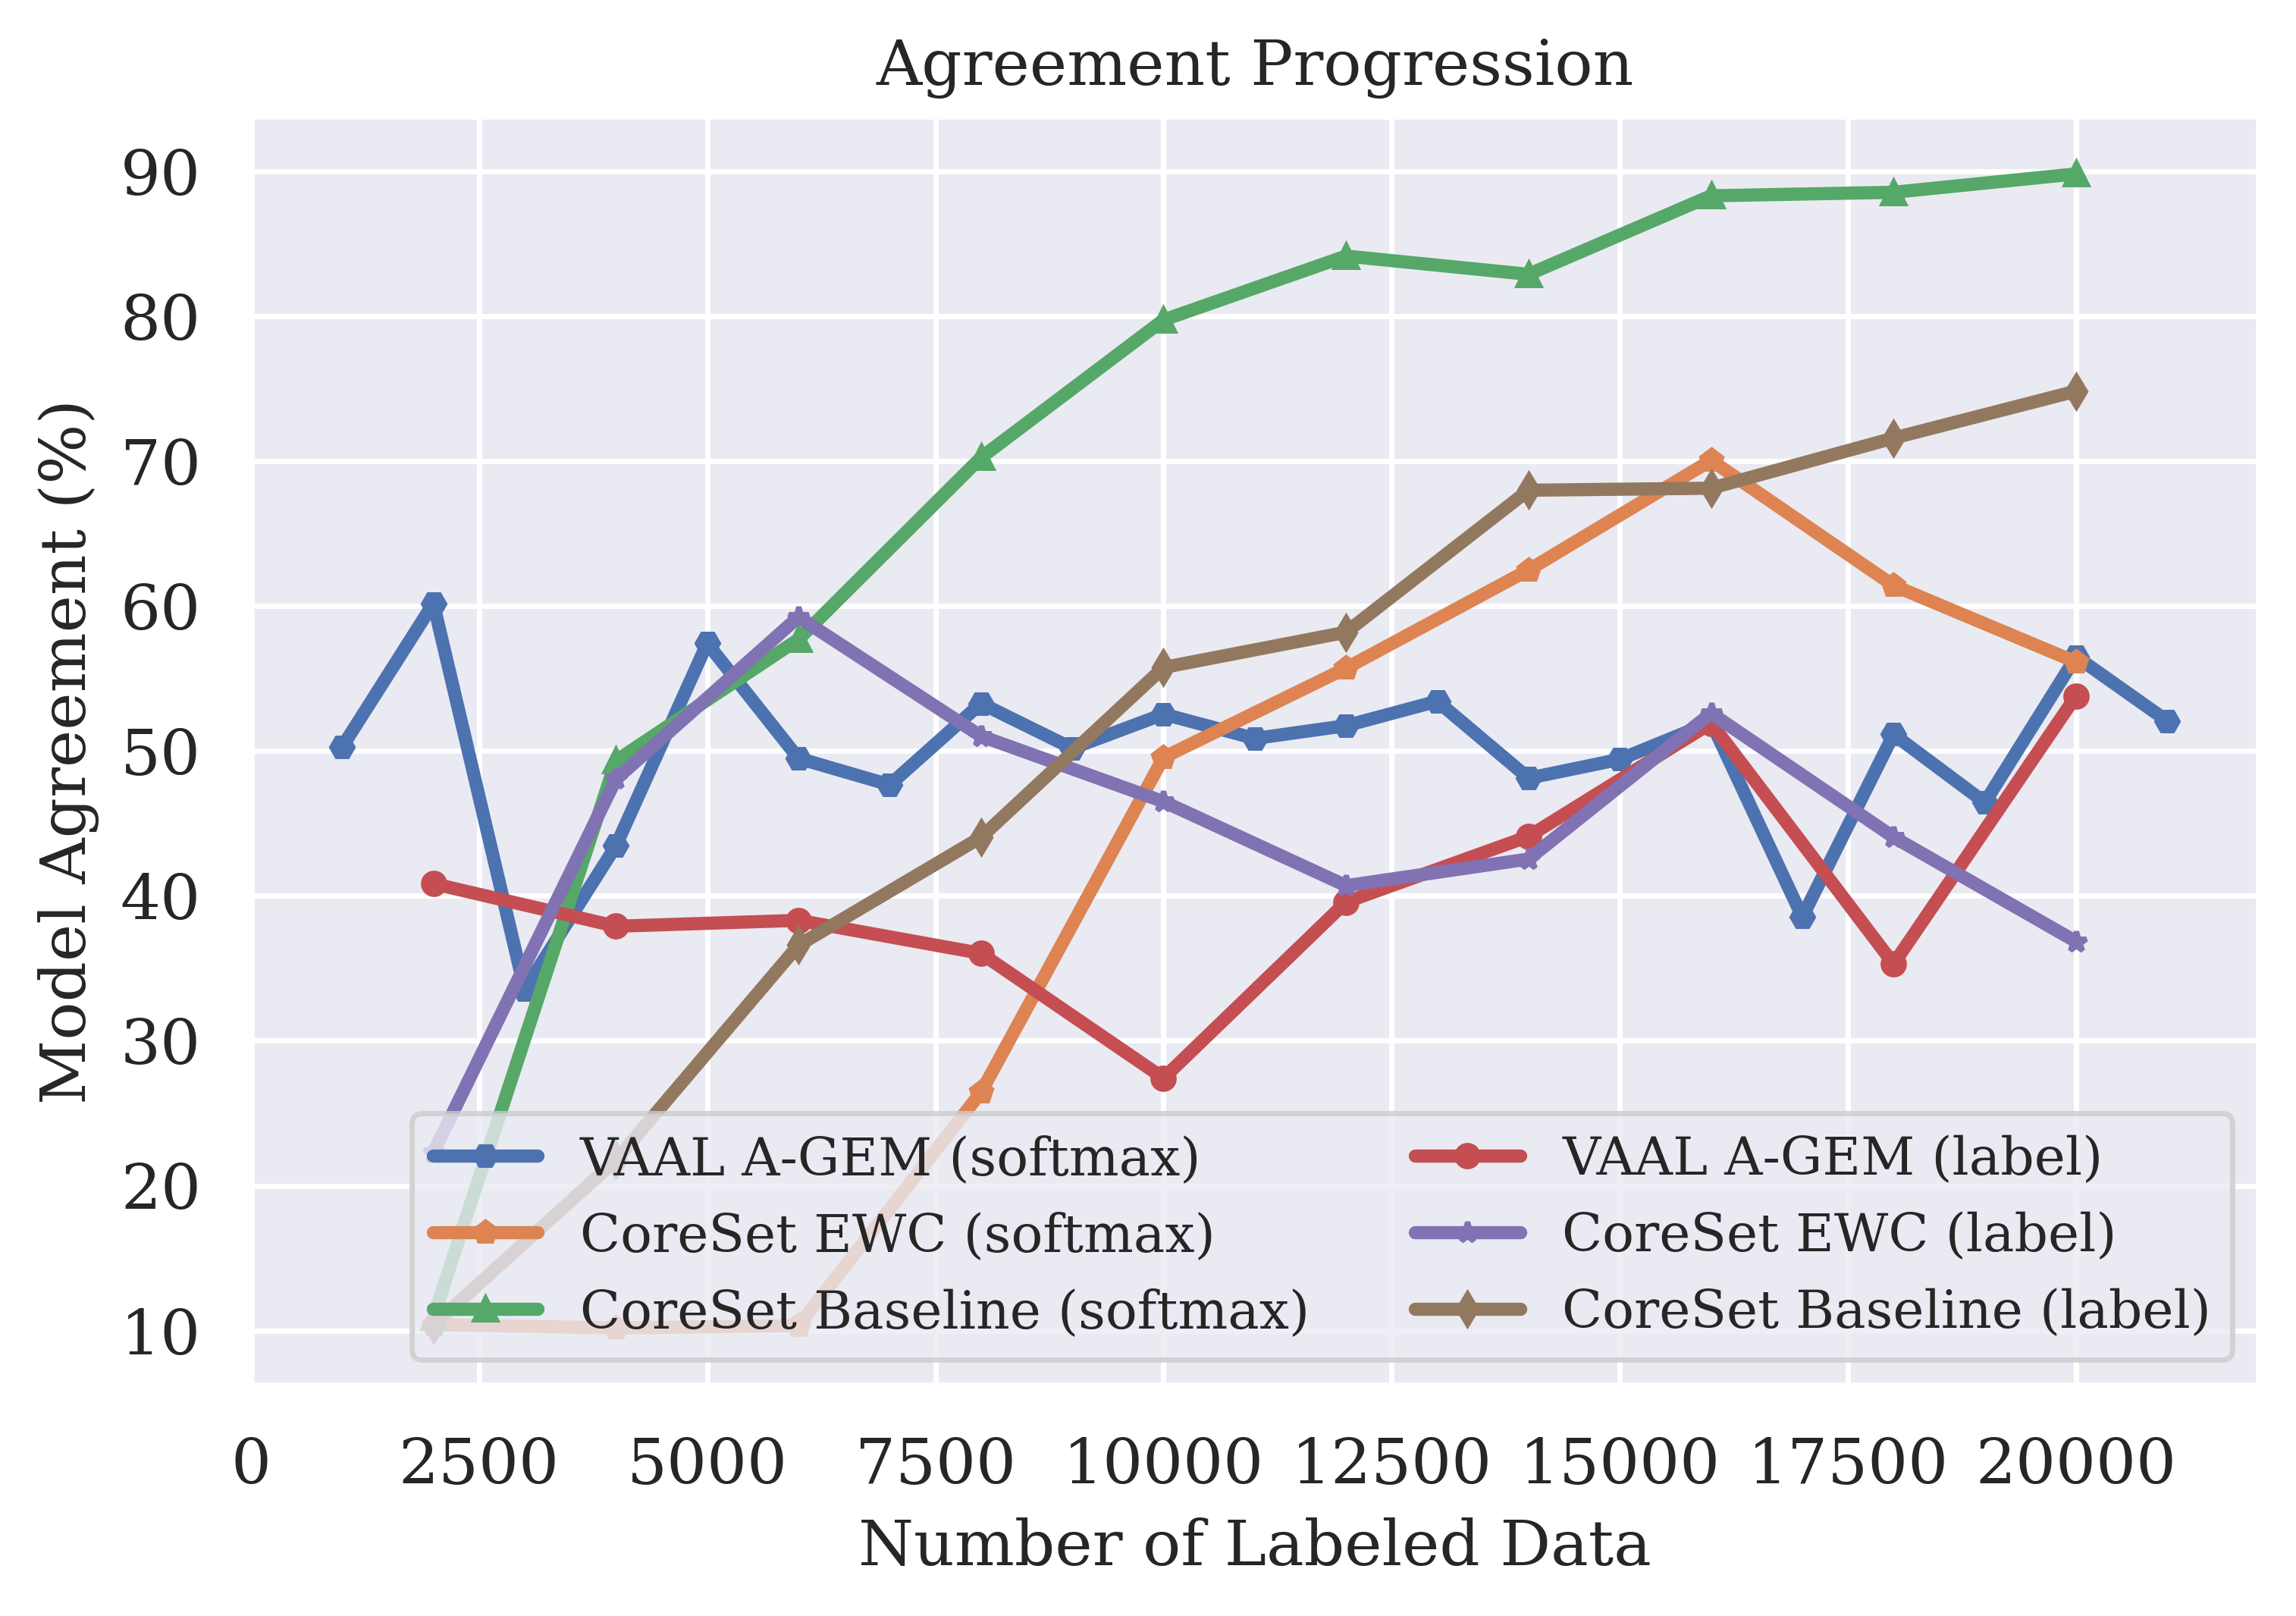
\includegraphics[width=0.316\linewidth]{images/results_CALMS/mnist_vaal_agem.png} 
    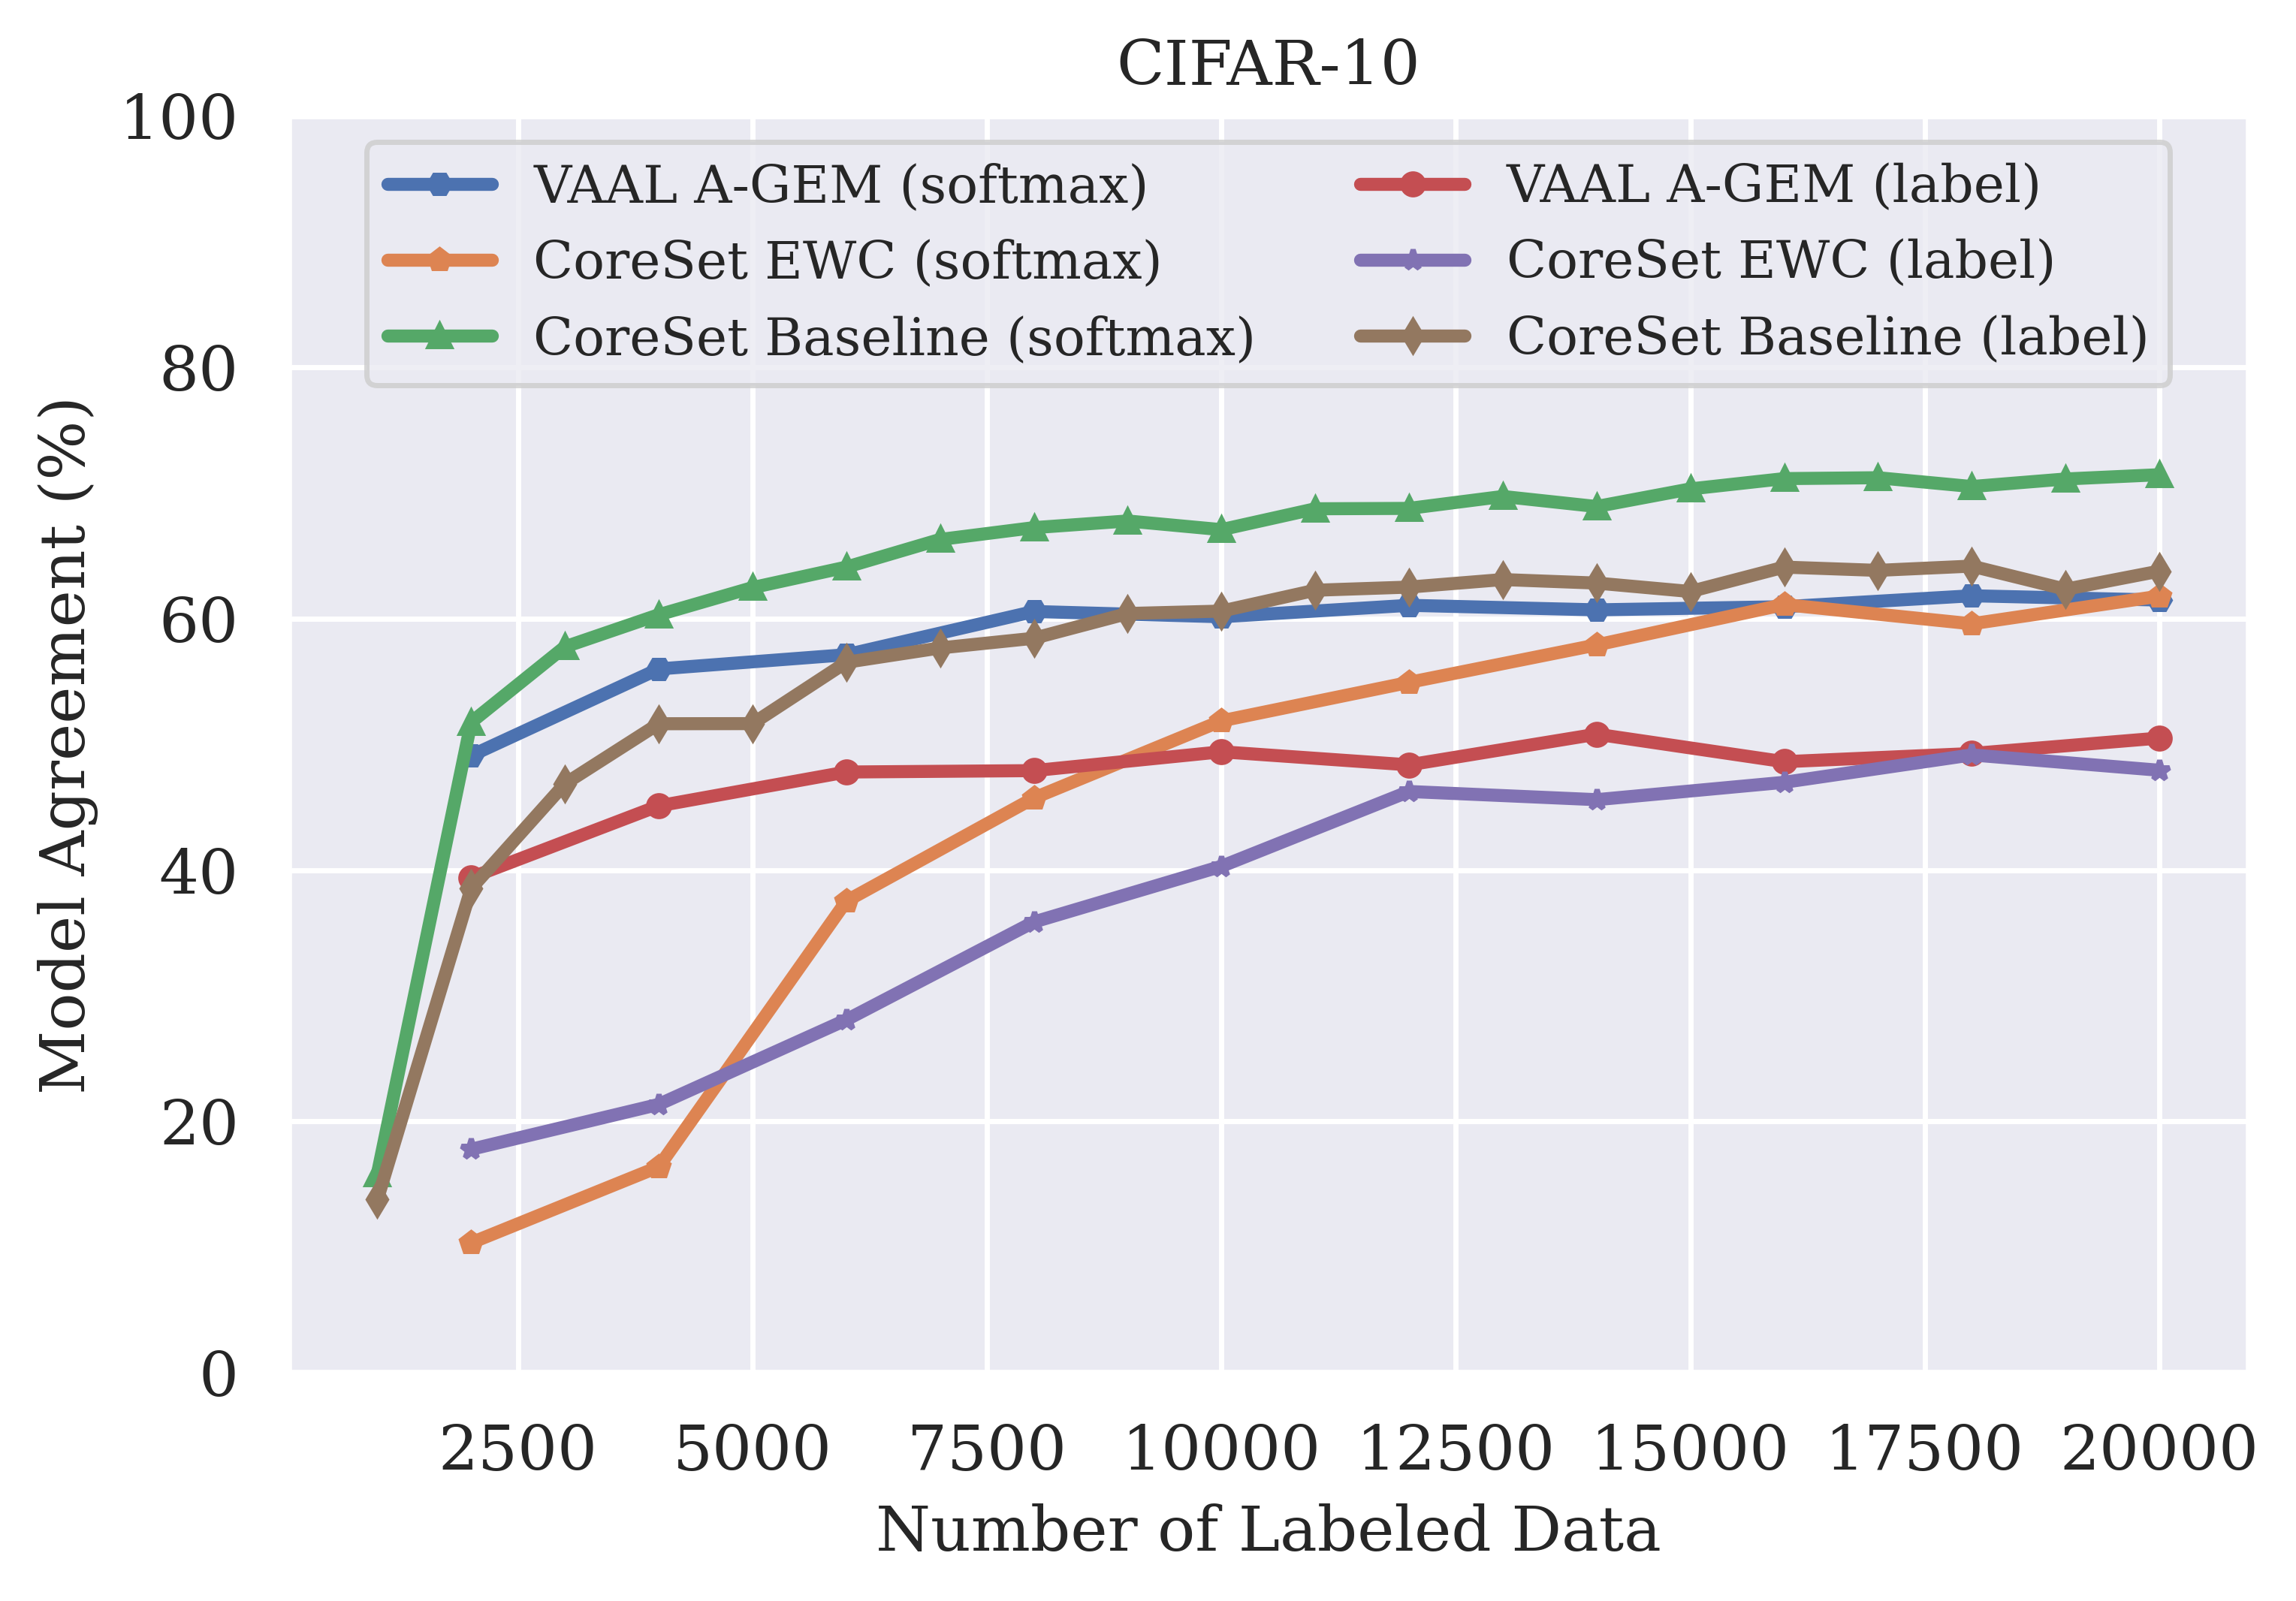
\includegraphics[width=0.32\linewidth]{images/results_CALMS/cifar_vaal_agem.png}
    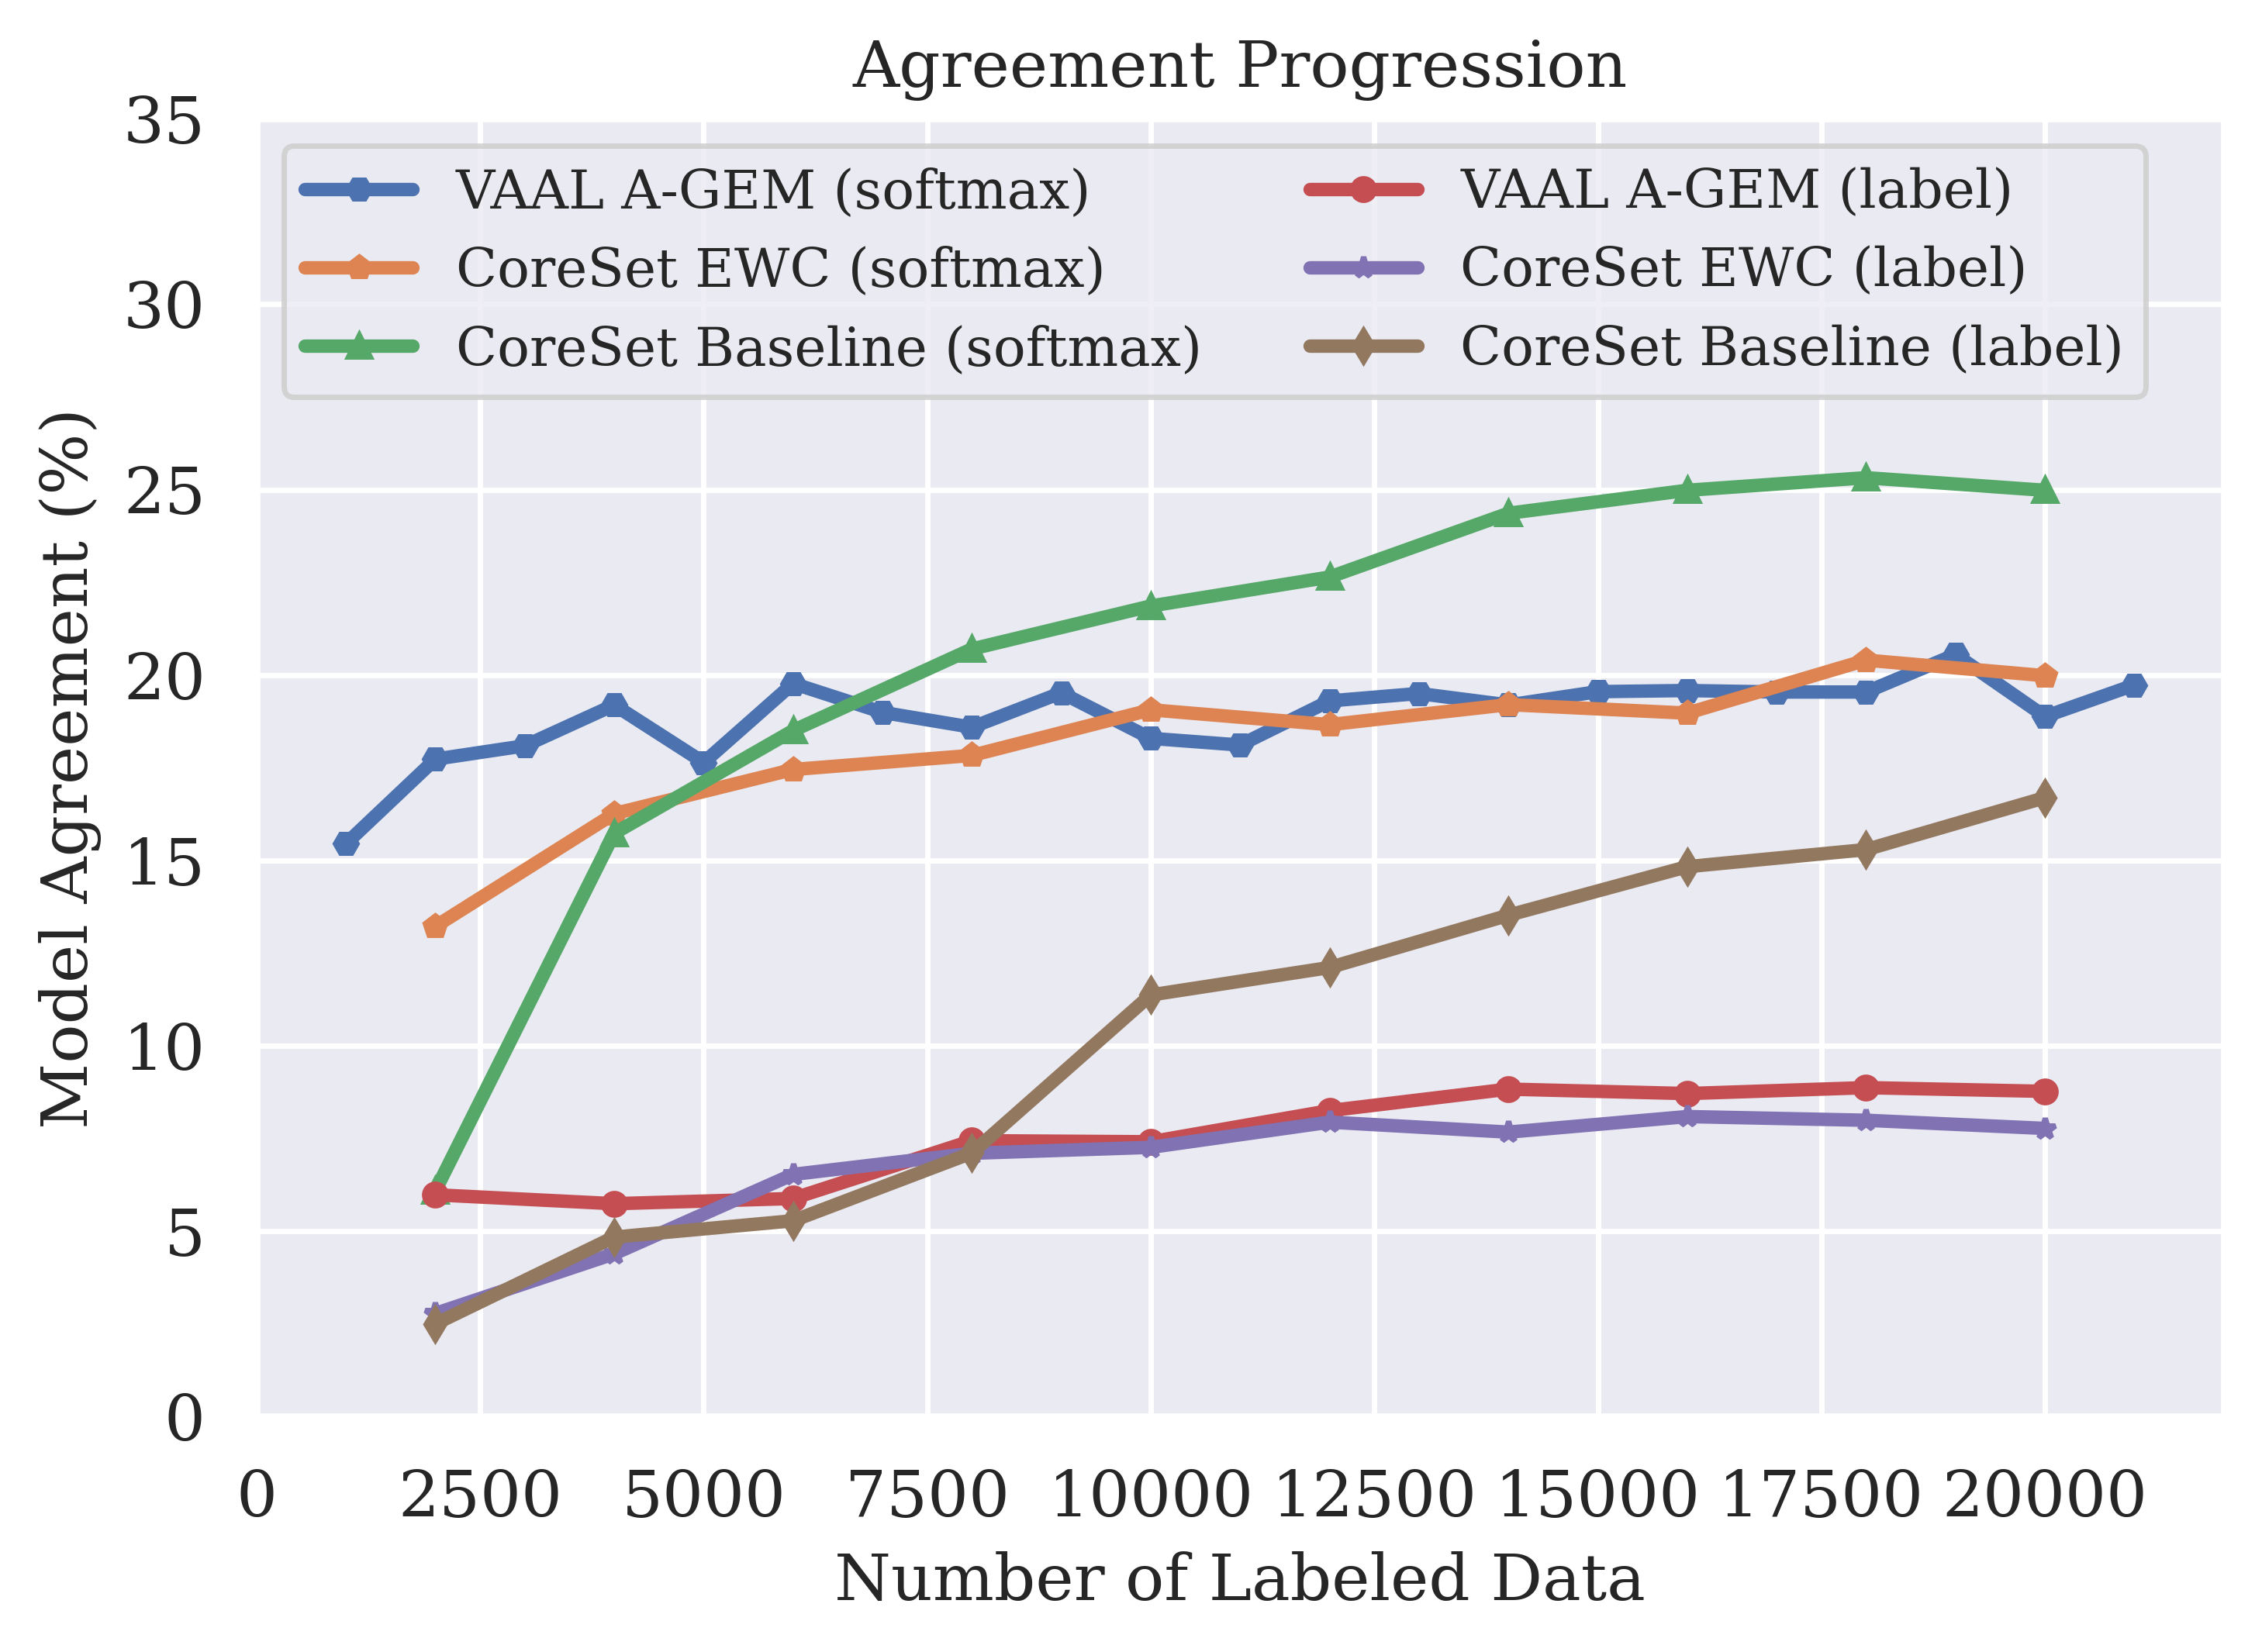
\includegraphics[width=0.316\linewidth]{images/results_CALMS/cifar100_vaal_agem.png}
    \caption{Agreement comparison for model stealing using \gls{vaal} and \gls{a-gem}.}
    \label{fig:CALMS_VAAL_AGEM}
\end{figure}

\subsection{Effect of Data Augmentation on Model Stealing Attacks}
\label{sec:Appendix:EffectDataAugmentation}

While we managed to reproduce the findings of Pal et al. for CIFAR-10, we failed to do so for MNIST. Since multiple training hyperparameters of the experiments
presented in ActiveThief were not disclosed by the authors, we experiment with different combinations of hyperparameters, including varying the optimizer,
the learning rate, the number of training epochs, the batch size, and switching between cold start and warm start for active learning. Sadly, we were still
not able to reproduce the results of ActiveThief on MNIST. After conducting the experiments in section \ref{sec:Evaluation:MS}, we decided to investigate
another hyperparameter: training with or without data augmentation. For this set of experiments, we leave all hyperparameters equal to the previous experiments,
apart from data augmentation. We underline that using or not using data augmentation for model stealing refers to the thief dataset, not the target
model dataset. Training the target model is always done using data augmentation. We perform the same model stealing attacks as before, using MNIST and
CIFAR-10 as the target model dataset and present the results in figure \ref{fig:Evaluation:Results:CAL:EffectAugmentation}. When performing model stealing attacks
without data augmentation on CIFAR-10, we notice that model agreement, both for active learning and continual active learning, is significantly lower than
when using data augmentation. In this scenario, continual active learning with data augmentation performs on par with active learning without data augmentation.
However, when using MNIST as the target model dataset, the results are reversed. Here, model agreement is significantly lower when using data augmentation.
More importantly, continual active learning without data augmentation shows performance comparable to active learning with data augmentation. \par

\begin{figure}[!htb]
    \centering
    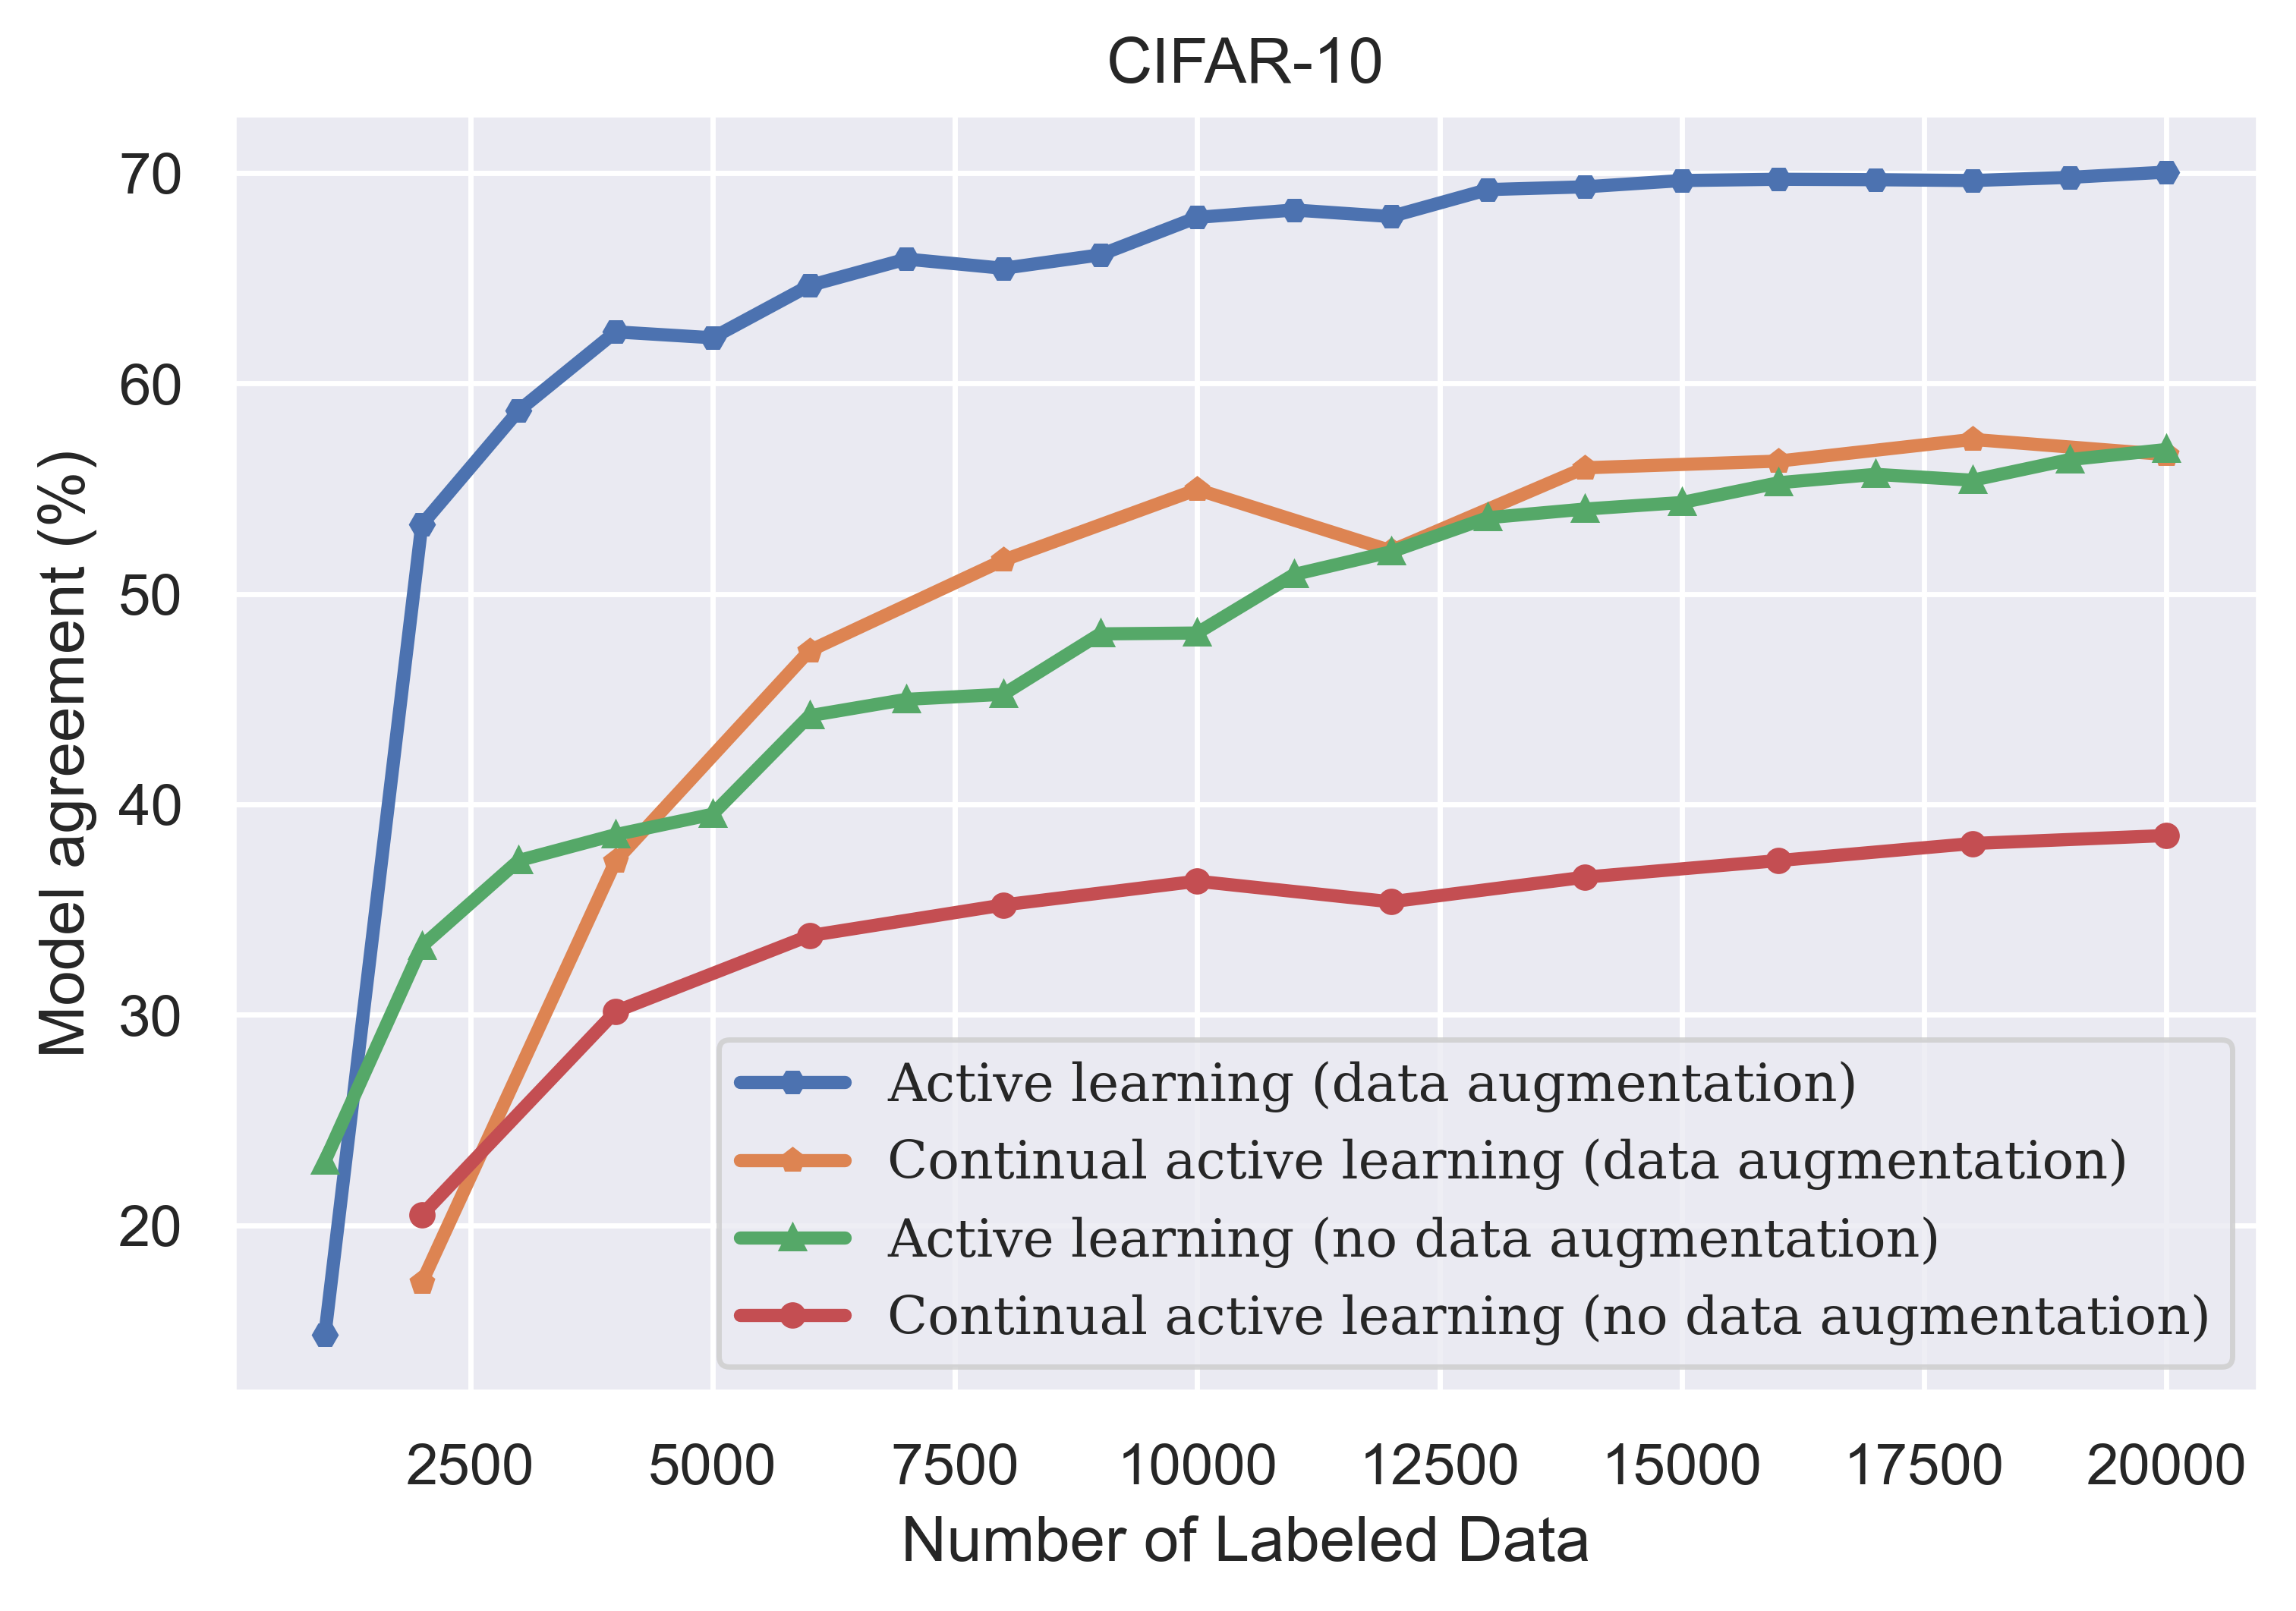
\includegraphics[width=0.48\linewidth]{images/results_CALMS/data_augmentation_cifar.png} \hfill
    \includegraphics[width=0.48\linewidth]{images/results_CALMS/data_augmentation_mnist.png}
    \caption{Comparison of model agreement with and without data augmentation.}
    \label{fig:Evaluation:Results:CAL:EffectAugmentation}
\end{figure}

